% =====================================================================================
%  safe_prompt_fields.tex
%
%  Distilled version of flow_matching_safe_set_POC.tex, reorganised around one idea:
%  the velocity field of a new prompt is constrained to the order-1 Wasserstein conformal
%  region built from the fields of safe prompts, for flow-matching models that are linear
%  in their parameters.  The original note is kept unchanged as the full record.
%  Build (from this folder):
%      pdflatex safe_prompt_fields && bibtex safe_prompt_fields
%      && pdflatex safe_prompt_fields && pdflatex safe_prompt_fields
%  Every number in Section 8 is copied by hand from tables/numbers.tex and tables/tab_*.tex
%  (written by code/make_tables.py from results/); every number in Sections 3, 9 and 10 is a macro
%  of tables/e1_numbers.tex, e1_walk_numbers.tex, reflow_numbers.tex or e2_numbers.tex, and every number
%  in Section 11 a macro of tables/e3_numbers.tex or a table body tables/e3_*.tex (code/e3_figures.py).
%  Revised on 14 October 2026 after the audit safe_prompt_fields_audit.tex; the audited version is
%  archived in archive/2026-10-14_pre_audit/.
% =====================================================================================
\documentclass{article}
\usepackage[preprint]{custom_2020}
\usepackage{amsmath}
\usepackage{stmaryrd}
\usepackage{tgtermes}
\usepackage[dvipsnames]{xcolor}
\usepackage{bm}
\usepackage{bbm}
\usepackage[hidelinks]{hyperref}
\usepackage{amssymb,amsfonts}
\usepackage{caption}
\usepackage{graphicx}
\usepackage{booktabs}
\usepackage{mathtools}
\usepackage{enumitem}
\usepackage{placeins}

\DeclareMathOperator*{\argmin}{arg\,min}
\DeclareMathOperator{\E}{\mathbb{E}}
\DeclareMathOperator{\dist}{dist}
\DeclareMathOperator{\conv}{conv}
\newcommand{\RR}{\mathbb{R}}
\newcommand{\PP}{\mathbbm{P}}
\newcommand{\cD}{\mathcal{D}}
\newcommand{\cE}{\mathcal{E}}
\newcommand{\cL}{\mathcal{L}}
\newcommand{\cN}{\mathcal{N}}
\newcommand{\bth}{\boldsymbol{\theta}}
\newcommand{\bx}{\mathbf{x}}
\newcommand{\by}{\mathbf{y}}
\newcommand{\bu}{\mathbf{u}}
\newcommand{\bb}{\mathbf{b}}
\newcommand{\ba}{\mathbf{a}}
\newcommand{\be}{\mathbf{e}}
\newcommand{\bxi}{\boldsymbol{\xi}}
\newcommand{\TV}{\mathrm{TV}}
\newcommand{\KL}{\mathrm{KL}}
\newcommand{\kl}{\mathrm{kl}}
\newcommand{\Tbar}{\bar{\Theta}}
\newcommand{\vstar}{v^{\star}}

\usepackage{natbib}
 \bibpunct[, ]{(}{)}{,}{a}{}{,}%
 \def\bibfont{\small}%
 \def\bibsep{\smallskipamount}%
 \def\bibhang{24pt}%
 \def\newblock{\ }%
 \def\BIBand{and}%

\usepackage{amsthm}
\theoremstyle{plain}
\newtheorem{theorem}{Theorem}[section]
\newtheorem{lemma}[theorem]{Lemma}
\newtheorem{proposition}[theorem]{Proposition}
\newtheorem{corollary}[theorem]{Corollary}
\newtheorem{definition}[theorem]{Definition}
\newtheorem{assumption}[theorem]{Assumption}
\theoremstyle{remark}
\newtheorem{remark}[theorem]{Remark}

\setlist{itemsep=1pt,topsep=3pt}
\newcommand{\pairKLAmed}{0.067}
\newcommand{\pairKLAninety}{0.257}
\newcommand{\pALmean}{8.3\times 10^{-6}}
\newcommand{\pairKLDmed}{0.378}
\newcommand{\pairKLDninety}{0.755}
\newcommand{\pALDmean}{0.0004}
\newcommand{\pALCmean}{0.0017}
\newcommand{\covAF}{0.897}
\newcommand{\covAK}{0.898}
\newcommand{\exclAFthree}{0.42}
\newcommand{\exclAKthree}{1.00}
\newcommand{\exclAKone}{0.83}
\newcommand{\exclAFone}{0.19}
\newcommand{\exclCrefthree}{0.15}
\newcommand{\exclConthree}{0.55}
\newcommand{\exclDfwdthree}{0.17}
\newcommand{\exclDrevthree}{0.55}
\newcommand{\exclDfwdten}{0.69}
\newcommand{\exclCononeP}{0.133}
\newcommand{\exclConthreeP}{0.552}
\newcommand{\exclDrevoneP}{0.129}
\newcommand{\exclDrevthreeP}{0.546}
\newcommand{\certAKmed}{0.031}
\newcommand{\certAFmed}{0.283}
\newcommand{\certDrevmed}{0.134}
\newcommand{\certDfwdmed}{0.553}
\newcommand{\insideAKmed}{0.0123}
\newcommand{\insideAFmed}{0.0324}
\newcommand{\insideAFmax}{0.0947}
\newcommand{\insideDrevmed}{0.0145}
\newcommand{\insideDfwdmed}{0.0707}
\newcommand{\geoCrefclean}{0.28}
\newcommand{\geoConclean}{0.35}
\newcommand{\winCrefclean}{32}
\newcommand{\winConclean}{32}
\newcommand{\geoCrefcont}{0.21}
\newcommand{\geoConcont}{0.20}
\newcommand{\winCrefcont}{32}
\newcommand{\winConcont}{32}
\newcommand{\ntasks}{32}
\newcommand{\pAUcont}{0.138}
\newcommand{\pACrefcont}{0.047}
\newcommand{\pAConcont}{0.025}
\newcommand{\pASten}{0.0087}
\newcommand{\backoffmax}{0.011}
\newcommand{\backofffrac}{0.70}
\newcommand{\socptime}{0.31}
\newcommand{\epsref}{0.0182}
\newcommand{\epson}{0.0193}
\newcommand{\exampletask}{8}
\newcommand{\exUpA}{0.133}
\newcommand{\exCrefpA}{0.029}
\newcommand{\exConpA}{0.013}
\newcommand{\exSpA}{0.009}
\newcommand{\excentrepA}{0.001}
\newcommand{\exoraclepA}{0.003}
\newcommand{\excentresref}{0.55}
\newcommand{\excentreson}{0.54}
\newcommand{\lipmin}{52}
\newcommand{\lipmax}{53}
\newcommand{\gronwalllog}{15}

\newcommand{\eoneSafePAA}{0.0024}
\newcommand{\eoneZetaA}{1.93}
\newcommand{\eonePAAa}{0.005}
\newcommand{\eonePAAb}{0.014}
\newcommand{\eonePAAc}{0.074}
\newcommand{\eonePAAd}{0.253}
\newcommand{\eoneSafePAB}{0.0046}
\newcommand{\eoneZetaB}{0.26}
\newcommand{\eonePABa}{0.007}
\newcommand{\eonePABb}{0.015}
\newcommand{\eonePABc}{0.065}
\newcommand{\eonePABd}{0.237}
\newcommand{\eoneTruePAd}{0.284}
\newcommand{\eoneOneStepPA}{0.0176}
\newcommand{\eoneCovAT}{0.897}
\newcommand{\eoneExATb}{0.07}
\newcommand{\eoneExATc}{0.24}
\newcommand{\eoneExATd}{1.00}
\newcommand{\eoneBudgetAT}{0.83}
\newcommand{\eoneCovAZ}{0.900}
\newcommand{\eoneExAZb}{0.20}
\newcommand{\eoneExAZc}{0.82}
\newcommand{\eoneExAZd}{0.95}
\newcommand{\eoneBudgetAZ}{0.50}
\newcommand{\eoneCovAR}{0.900}
\newcommand{\eoneExARb}{0.09}
\newcommand{\eoneExARc}{0.16}
\newcommand{\eoneExARd}{0.48}
\newcommand{\eoneBudgetAR}{0.98}
\newcommand{\eoneCovAE}{0.907}
\newcommand{\eoneExAEb}{0.12}
\newcommand{\eoneExAEc}{0.29}
\newcommand{\eoneExAEd}{1.00}
\newcommand{\eoneBudgetAE}{1.61}
\newcommand{\eoneCovBT}{0.900}
\newcommand{\eoneExBTb}{0.10}
\newcommand{\eoneExBTc}{0.29}
\newcommand{\eoneExBTd}{1.00}
\newcommand{\eoneBudgetBT}{0.68}
\newcommand{\eoneCovBZ}{0.901}
\newcommand{\eoneExBZb}{0.10}
\newcommand{\eoneExBZc}{0.29}
\newcommand{\eoneExBZd}{1.00}
\newcommand{\eoneBudgetBZ}{0.58}
\newcommand{\eoneCovBR}{0.900}
\newcommand{\eoneExBRb}{0.12}
\newcommand{\eoneExBRc}{0.32}
\newcommand{\eoneExBRd}{1.00}
\newcommand{\eoneBudgetBR}{0.63}
\newcommand{\eoneCovBE}{0.907}
\newcommand{\eoneExBEb}{0.12}
\newcommand{\eoneExBEc}{0.29}
\newcommand{\eoneExBEd}{1.00}
\newcommand{\eoneBudgetBE}{1.61}
\newcommand{\eoneLfourUd}{0.03}
\newcommand{\eoneLeightUd}{0.02}
\newcommand{\eoneKnnLtwoc}{0.73}
\newcommand{\eoneKnnLonec}{0.98}
\newcommand{\eoneKnnLfourc}{0.40}
\newcommand{\eoneKnnTruncc}{0.99}
\newcommand{\eoneKnnTailb}{0.29}
\newcommand{\eoneKnnTailCov}{0.918}
\newcommand{\eonePlugFail}{0.4\%}
\newcommand{\eonePlugMax}{3.7}
\newcommand{\eoneMarkovMed}{0.99}
\newcommand{\eoneRegionWorst}{0.189}
\newcommand{\eoneOneStepRectOne}{0.97}
\newcommand{\eoneMmdA}{3.3}
\newcommand{\eoneMmdB}{8.1}
\newcommand{\eoneMmdC}{34.9}
\newcommand{\eoneTwoPAasWritten}{0.142}
\newcommand{\eoneTwoPAtrunc}{0.032}
\newcommand{\eoneTwoMmdAsWritten}{84}
\newcommand{\eoneTwoMmdTrunc}{28}
\newcommand{\eoneTwoMmdNone}{149}
\newcommand{\eoneTwoBudgetUL}{0.84}
\newcommand{\eoneTwoBudgetTrunc}{0.18}
\newcommand{\eoneTwoAttackUL}{0.186}
\newcommand{\eoneTwoAttackLone}{0.054}
\newcommand{\eoneTwoAttackTrunc}{0.051}
\newcommand{\eoneTwoAttackTail}{0.044}
\newcommand{\eoneTwoAttackEU}{1.000}
\newcommand{\eoneTwoAttackEknn}{0.974}
\newcommand{\eoneTwoPlugMin}{8\%}
\newcommand{\eoneTwoPlugMax}{28\%}
\newcommand{\eoneTwoTruncMaxRatio}{1.13}
\newcommand{\eoneTwoLoneMaxRatio}{8.5}
\newcommand{\eoneTwoCertTail}{0.077}
\newcommand{\eoneTwoCertTrunc}{0.29}
\newcommand{\eoneProbe}{136}
\newcommand{\eoneProbeNorm}{3.96}
\newcommand{\eoneProbeMaxT}{16.5}
\newcommand{\eoneEvalMaxT}{2.8\times10^{4}}
\newcommand{\eoneBlowSafe}{44}
\newcommand{\eoneBlowUns}{3}
\newcommand{\eoneShareMed}{6}
\newcommand{\eoneShareMean}{19}
\newcommand{\eoneShareNinety}{57}
\newcommand{\eonePrLfourUAlla}{0.17}
\newcommand{\eonePrLfourUAllb}{0.17}
\newcommand{\eonePrLfourUAllc}{0.08}
\newcommand{\eonePrLfourUAlld}{0.03}
\newcommand{\eonePrLfourUAllEps}{1.816}
\newcommand{\eonePrLfourUDropa}{0.07}
\newcommand{\eonePrLfourUDropb}{0.07}
\newcommand{\eonePrLfourUDropc}{0.30}
\newcommand{\eonePrLfourUDropd}{1.00}
\newcommand{\eonePrLfourUDropEps}{0.911}
\newcommand{\eonePrLeightUAlla}{0.18}
\newcommand{\eonePrLeightUAllb}{0.17}
\newcommand{\eonePrLeightUAllc}{0.08}
\newcommand{\eonePrLeightUAlld}{0.02}
\newcommand{\eonePrLeightUAllEps}{3.522}
\newcommand{\eonePrLeightUDropa}{0.08}
\newcommand{\eonePrLeightUDropb}{0.08}
\newcommand{\eonePrLeightUDropc}{0.18}
\newcommand{\eonePrLeightUDropd}{1.00}
\newcommand{\eonePrLeightUDropEps}{1.163}
\newcommand{\eonePrLtwoUAlla}{0.09}
\newcommand{\eonePrLtwoUAllb}{0.07}
\newcommand{\eonePrLtwoUAllc}{0.24}
\newcommand{\eonePrLtwoUAlld}{1.00}
\newcommand{\eonePrLtwoUAllEps}{0.829}
\newcommand{\eonePrLtwoUDropa}{0.07}
\newcommand{\eonePrLtwoUDropb}{0.08}
\newcommand{\eonePrLtwoUDropc}{0.33}
\newcommand{\eonePrLtwoUDropd}{1.00}
\newcommand{\eonePrLtwoUDropEps}{0.739}
\newcommand{\eonePrLtwoNAlla}{0.13}
\newcommand{\eonePrLtwoNAllb}{0.17}
\newcommand{\eonePrLtwoNAllc}{0.73}
\newcommand{\eonePrLtwoNAlld}{1.00}
\newcommand{\eonePrLtwoNAllEps}{0.377}
\newcommand{\eonePrLtwoNDropa}{0.11}
\newcommand{\eonePrLtwoNDropb}{0.20}
\newcommand{\eonePrLtwoNDropc}{1.00}
\newcommand{\eonePrLtwoNDropd}{1.00}
\newcommand{\eonePrLtwoNDropEps}{0.239}
\newcommand{\eonePrBudRatioDrop}{3.1}
\newcommand{\eonePrTwoLeightUAlld}{0.23}
\newcommand{\eoneFigCovMin}{0.897}
\newcommand{\eoneFigCovMax}{0.934}
\newcommand{\eoneKnnTailCovTwo}{0.934}
\newcommand{\eoneTailProbesOne}{11}
\newcommand{\eoneTailProbesTwo}{2}
\newcommand{\eoneNonTailCovMax}{0.908}
\newcommand{\eoneFloorAT}{0.33}
\newcommand{\eoneTypicalAT}{0.68}
\newcommand{\eoneExcessa}{0.0023}
\newcommand{\eoneTargeta}{0.0095}
\newcommand{\eoneRealiseda}{24}
\newcommand{\eoneExcessb}{0.0112}
\newcommand{\eoneTargetb}{0.0284}
\newcommand{\eoneRealisedb}{40}
\newcommand{\eoneMixcheck}{6\times10^{-13}}
\newcommand{\eoneDirUL}{0.084}
\newcommand{\eoneDirNear}{0.024}
\newcommand{\eoneSlackBound}{0.30}
\newcommand{\eoneSlackPA}{0.030}
\newcommand{\eoneVerDelta}{0.05}
\newcommand{\eoneVerL}{2000}
\newcommand{\eoneVerLbig}{10{,}000}
\newcommand{\eoneVerHoeff}{0.033}
\newcommand{\eoneVerViol}{0}
\newcommand{\eoneVerN}{5600}
\newcommand{\eoneVerOverMax}{0.0\%}
\newcommand{\eoneVerOneTrPA}{0.014}
\newcommand{\eoneVerOneTrMmd}{22}
\newcommand{\eoneVerOneTrAlt}{0.20}
\newcommand{\eoneVerOneTrFall}{0.00}
\newcommand{\eoneVerOneTrBound}{0.304}
\newcommand{\eoneVerOneTailPA}{0.019}
\newcommand{\eoneVerOneTailMmd}{36}
\newcommand{\eoneVerOneTailAlt}{0.17}
\newcommand{\eoneVerOneTailFall}{0.00}
\newcommand{\eoneVerOneTailBound}{0.079}
\newcommand{\eoneVerTwoTrPA}{0.015}
\newcommand{\eoneVerTwoTrMmd}{32}
\newcommand{\eoneVerTwoTrAlt}{0.24}
\newcommand{\eoneVerTwoTrFall}{0.00}
\newcommand{\eoneVerTwoTrBound}{0.297}
\newcommand{\eoneVerTwoTailPA}{0.020}
\newcommand{\eoneVerTwoTailMmd}{49}
\newcommand{\eoneVerTwoTailAlt}{0.19}
\newcommand{\eoneVerTwoTailFall}{0.16}
\newcommand{\eoneVerTwoTailBound}{0.061}

% written by code/e1_walkthrough.py
\newcommand{\ewPhi}{10.1}
\newcommand{\ewRho}{1.81}
\newcommand{\ewBudRatioOne}{2.2}
\newcommand{\ewBudRatioTwo}{3.6}
\newcommand{\ewTruePAb}{0.029}
\newcommand{\ewTruePAc}{0.094}
\newcommand{\ewTruePAd}{0.283}
\newcommand{\ewMassA}{0.26}
\newcommand{\ewDispA}{1.1}
\newcommand{\ewDispNotA}{0.16}
\newcommand{\ewZetaOne}{1.81}
\newcommand{\ewOneStepAOne}{96}
\newcommand{\ewZetaTwo}{0.17}
\newcommand{\ewOneStepATwo}{3}
\newcommand{\ewSwitch}{38}
\newcommand{\ewRotA}{33}
\newcommand{\ewAngA}{-22}
\newcommand{\ewRotNear}{1.2}
\newcommand{\ewDLtwoNear}{0.08}
\newcommand{\ewDLoneNear}{0.06}
\newcommand{\ewDTrNear}{0.06}
\newcommand{\ewDTailNear}{0.00}
\newcommand{\ewDLtwoRot}{1.01}
\newcommand{\ewDLoneRot}{0.96}
\newcommand{\ewDTrRot}{0.85}
\newcommand{\ewDTailRot}{0.95}
\newcommand{\ewDLtwoUns}{0.68}
\newcommand{\ewDLoneUns}{0.49}
\newcommand{\ewDTrUns}{0.45}
\newcommand{\ewDTailUns}{0.39}
\newcommand{\ewCovU}{93}
\newcommand{\ewSafeLoU}{0.66}
\newcommand{\ewSafeHiU}{1.02}
\newcommand{\ewExUa}{5}
\newcommand{\ewExUb}{1}
\newcommand{\ewExUc}{7}
\newcommand{\ewExUd}{100}
\newcommand{\ewScUzero}{0.75}
\newcommand{\ewScUone}{0.90}
\newcommand{\ewEpsU}{0.86}
\newcommand{\ewCovK}{88}
\newcommand{\ewExKa}{15}
\newcommand{\ewExKb}{26}
\newcommand{\ewExKc}{100}
\newcommand{\ewExKd}{100}
\newcommand{\ewScKzero}{0.33}
\newcommand{\ewScKone}{1.42}
\newcommand{\ewEpsK}{0.18}
\newcommand{\ewSlicePAa}{0.256}
\newcommand{\ewSlicePAb}{0.141}
\newcommand{\ewSlicePAc}{0.028}
\newcommand{\ewSlicePAd}{0.007}
\newcommand{\ewSlicePAe}{0.002}
\newcommand{\ewSlicePAf}{0.000}
\newcommand{\ewSliceMaxU}{0.19}
\newcommand{\ewSliceMaxK}{0.034}
\newcommand{\ewKapU}{0.23}
\newcommand{\ewKapK}{0.72}
\newcommand{\ewAlphaU}{0.77}
\newcommand{\ewAlphaK}{0.28}
\newcommand{\ewRotSlice}{31}
\newcommand{\ewCertU}{0.99}
\newcommand{\ewCertRU}{1.09}
\newcommand{\ewCertQU}{0.19}
\newcommand{\ewCertPAU}{0.141}
\newcommand{\ewCertK}{0.32}
\newcommand{\ewCertRK}{0.73}
\newcommand{\ewCertQK}{0.08}
\newcommand{\ewCertPAK}{0.028}
\newcommand{\ewCertBudgetK}{0.175}
\newcommand{\ewCertFar}{0}
\newcommand{\ewAtkPrompt}{1.000}
\newcommand{\ewAtkWritten}{0.186}
\newcommand{\ewAtkImproved}{0.051}
\newcommand{\ewAtkEmbNear}{1.07}
\newcommand{\ewAtkEmbMed}{1.28}
\newcommand{\ewAtkScU}{2.3}
\newcommand{\ewAtkScK}{5.6}

% written by code/make_reflow_figure.py
\newcommand{\rfVind}{3.8}
\newcommand{\rfVrefl}{0.002}
\newcommand{\rfCostInd}{6.18}
\newcommand{\rfCostRefl}{0.97}
\newcommand{\rfCurv}{1.44}
\newcommand{\rfDecrease}{5.21}
\newcommand{\rfSum}{5.25}
\newcommand{\rfVmin}{1.6}
\newcommand{\rfVzero}{4.3}
\newcommand{\rfEoneDropped}{0.04}
\newcommand{\rfEoneMax}{2.5\times10^{5}}

% written by code/e2_figures.py
\newcommand{\etScEstatic}{0.76}
\newcommand{\etMapMaxEstatic}{0.20}
\newcommand{\etMapEstatic}{25}
\newcommand{\etMapSafeEstatic}{95}
\newcommand{\etWEtop}{0.16}
\newcommand{\etWEtopthree}{0.47}
\newcommand{\etScEadaptive}{1.37}
\newcommand{\etMapMaxEadaptive}{0.06}
\newcommand{\etMapEadaptive}{2}
\newcommand{\etMapSafeEadaptive}{100}
\newcommand{\etScFstatic}{0.77}
\newcommand{\etMapMaxTRstatic}{0.27}
\newcommand{\etMapTRstatic}{27}
\newcommand{\etMapSafeTRstatic}{89}
\newcommand{\etWFtop}{0.59}
\newcommand{\etWFtopthree}{0.87}
\newcommand{\etScFadaptive}{1.57}
\newcommand{\etMapMaxTRadaptive}{0.04}
\newcommand{\etMapTRadaptive}{0}
\newcommand{\etMapSafeTRadaptive}{95}
\newcommand{\etTuneGap}{0.05}
\newcommand{\etTuneRegret}{0.005}
\newcommand{\etNearGap}{0.004}
\newcommand{\etDensEA}{0.16}
\newcommand{\etDensUEA}{0.12}
\newcommand{\etEpsEA}{0.63}
\newcommand{\etEpsUEA}{1.60}
\newcommand{\etDensEB}{0.99}
\newcommand{\etDensUEB}{0.13}
\newcommand{\etEpsEB}{0.22}
\newcommand{\etEpsUEB}{1.57}
\newcommand{\etDensOneE}{0.17}
\newcommand{\etDensFA}{0.20}
\newcommand{\etDensUFA}{0.13}
\newcommand{\etEpsFA}{0.20}
\newcommand{\etEpsUFA}{0.59}
\newcommand{\etDensFB}{1.00}
\newcommand{\etDensUFB}{0.15}
\newcommand{\etEpsFB}{0.08}
\newcommand{\etEpsUFB}{0.58}
\newcommand{\etDensOneF}{0.24}
\newcommand{\etDensPA}{0.21}
\newcommand{\etDensUPA}{0.14}
\newcommand{\etEpsPA}{0.15}
\newcommand{\etEpsUPA}{0.58}
\newcommand{\etDensPB}{1.00}
\newcommand{\etDensUPB}{0.16}
\newcommand{\etEpsPB}{0.07}
\newcommand{\etEpsUPB}{0.57}
\newcommand{\etDensOneP}{0.26}
\newcommand{\etAtkOneES}{1.000}
\newcommand{\etAtkMedOneES}{0.983}
\newcommand{\etEnfOneES}{0.049}
\newcommand{\etMmdOneES}{28}
\newcommand{\etAtkOneEA}{0.976}
\newcommand{\etAtkMedOneEA}{0.920}
\newcommand{\etEnfOneEA}{0.009}
\newcommand{\etMmdOneEA}{11}
\newcommand{\etAtkOneMHS}{0.003}
\newcommand{\etAtkMedOneMHS}{0.000}
\newcommand{\etDirOneMHS}{0.026}
\newcommand{\etEnfOneMHS}{0.001}
\newcommand{\etMmdOneMHS}{91}
\newcommand{\etAtkOneMHA}{0.004}
\newcommand{\etAtkMedOneMHA}{0.000}
\newcommand{\etDirOneMHA}{0.044}
\newcommand{\etEnfOneMHA}{0.001}
\newcommand{\etMmdOneMHA}{101}
\newcommand{\etAtkOnePBS}{0.262}
\newcommand{\etAtkMedOnePBS}{0.131}
\newcommand{\etDirOnePBS}{0.854}
\newcommand{\etEnfOnePBS}{0.132}
\newcommand{\etMmdOnePBS}{73}
\newcommand{\etAtkOnePBA}{0.030}
\newcommand{\etAtkMedOnePBA}{0.021}
\newcommand{\etDirOnePBA}{0.219}
\newcommand{\etEnfOnePBA}{0.019}
\newcommand{\etMmdOnePBA}{21}
\newcommand{\etAtkOneFS}{0.220}
\newcommand{\etAtkMedOneFS}{0.146}
\newcommand{\etDirOneFS}{0.071}
\newcommand{\etEnfOneFS}{0.077}
\newcommand{\etMmdOneFS}{49}
\newcommand{\etAtkOneFA}{0.036}
\newcommand{\etAtkMedOneFA}{0.020}
\newcommand{\etDirOneFA}{0.019}
\newcommand{\etEnfOneFA}{0.026}
\newcommand{\etMmdOneFA}{26}
\newcommand{\etAtkTwoES}{0.655}
\newcommand{\etAtkMedTwoES}{0.537}
\newcommand{\etEnfTwoES}{0.061}
\newcommand{\etMmdTwoES}{78}
\newcommand{\etAtkTwoEA}{0.496}
\newcommand{\etAtkMedTwoEA}{0.228}
\newcommand{\etEnfTwoEA}{0.027}
\newcommand{\etMmdTwoEA}{47}
\newcommand{\etAtkTwoMHS}{0.016}
\newcommand{\etAtkMedTwoMHS}{0.015}
\newcommand{\etDirTwoMHS}{0.042}
\newcommand{\etEnfTwoMHS}{0.015}
\newcommand{\etMmdTwoMHS}{97}
\newcommand{\etAtkTwoMHA}{0.023}
\newcommand{\etAtkMedTwoMHA}{0.015}
\newcommand{\etDirTwoMHA}{0.056}
\newcommand{\etEnfTwoMHA}{0.015}
\newcommand{\etMmdTwoMHA}{101}
\newcommand{\etAtkTwoPBS}{0.099}
\newcommand{\etAtkMedTwoPBS}{0.086}
\newcommand{\etDirTwoPBS}{0.049}
\newcommand{\etEnfTwoPBS}{0.057}
\newcommand{\etMmdTwoPBS}{89}
\newcommand{\etAtkTwoPBA}{0.030}
\newcommand{\etAtkMedTwoPBA}{0.027}
\newcommand{\etDirTwoPBA}{0.024}
\newcommand{\etEnfTwoPBA}{0.034}
\newcommand{\etMmdTwoPBA}{76}
\newcommand{\etAtkTwoFS}{0.072}
\newcommand{\etAtkMedTwoFS}{0.064}
\newcommand{\etDirTwoFS}{0.047}
\newcommand{\etEnfTwoFS}{0.040}
\newcommand{\etMmdTwoFS}{75}
\newcommand{\etAtkTwoFA}{0.039}
\newcommand{\etAtkMedTwoFA}{0.029}
\newcommand{\etDirTwoFA}{0.029}
\newcommand{\etEnfTwoFA}{0.034}
\newcommand{\etMmdTwoFA}{72}
\newcommand{\etExESa}{0.11}
\newcommand{\etExESb}{0.12}
\newcommand{\etExESc}{0.30}
\newcommand{\etExESd}{1.00}
\newcommand{\etJES}{0.38}
\newcommand{\etCovES}{0.904}
\newcommand{\etExEAa}{0.11}
\newcommand{\etExEAb}{0.16}
\newcommand{\etExEAc}{0.99}
\newcommand{\etExEAd}{1.00}
\newcommand{\etJEA}{0.57}
\newcommand{\etCovEA}{0.905}
\newcommand{\etBestE}{0.3}
\newcommand{\etExFSa}{0.12}
\newcommand{\etExFSb}{0.13}
\newcommand{\etExFSc}{0.35}
\newcommand{\etExFSd}{0.98}
\newcommand{\etJFS}{0.40}
\newcommand{\etCovFS}{0.904}
\newcommand{\etExFAa}{0.11}
\newcommand{\etExFAb}{0.20}
\newcommand{\etExFAc}{0.99}
\newcommand{\etExFAd}{1.00}
\newcommand{\etJFA}{0.58}
\newcommand{\etCovFA}{0.906}
\newcommand{\etBestF}{0.2}
\newcommand{\etExPSa}{0.13}
\newcommand{\etExPSb}{0.14}
\newcommand{\etExPSc}{0.32}
\newcommand{\etExPSd}{1.00}
\newcommand{\etJPS}{0.40}
\newcommand{\etCovPS}{0.903}
\newcommand{\etExPAa}{0.11}
\newcommand{\etExPAb}{0.21}
\newcommand{\etExPAc}{1.00}
\newcommand{\etExPAd}{1.00}
\newcommand{\etJPA}{0.58}
\newcommand{\etCovPA}{0.907}
\newcommand{\etBestP}{0.1}
\newcommand{\etExSSa}{0.08}
\newcommand{\etExSSb}{0.15}
\newcommand{\etExSSc}{0.83}
\newcommand{\etExSSd}{0.91}
\newcommand{\etJSS}{0.49}
\newcommand{\etCovSS}{0.902}
\newcommand{\etExSAa}{0.13}
\newcommand{\etExSAb}{0.59}
\newcommand{\etExSAc}{1.00}
\newcommand{\etExSAd}{1.00}
\newcommand{\etJSA}{0.68}
\newcommand{\etCovSA}{0.905}
\newcommand{\etBestS}{0.2}
\newcommand{\etExLSa}{0.08}
\newcommand{\etExLSb}{0.08}
\newcommand{\etExLSc}{0.25}
\newcommand{\etExLSd}{0.99}
\newcommand{\etJLS}{0.35}
\newcommand{\etCovLS}{0.902}
\newcommand{\etExLAa}{0.09}
\newcommand{\etExLAb}{0.13}
\newcommand{\etExLAc}{0.74}
\newcommand{\etExLAd}{1.00}
\newcommand{\etJLA}{0.49}
\newcommand{\etCovLA}{0.902}
\newcommand{\etBestL}{0.1}
\newcommand{\etExTSa}{0.12}
\newcommand{\etExTSb}{0.14}
\newcommand{\etExTSc}{0.53}
\newcommand{\etExTSd}{1.00}
\newcommand{\etJTS}{0.45}
\newcommand{\etCovTS}{0.905}
\newcommand{\etExTAa}{0.12}
\newcommand{\etExTAb}{0.24}
\newcommand{\etExTAc}{0.99}
\newcommand{\etExTAd}{1.00}
\newcommand{\etJTA}{0.59}
\newcommand{\etCovTA}{0.904}
\newcommand{\etBestT}{0.3}
\newcommand{\etSpreadOne}{0.48}
\newcommand{\etDispOne}{0.24}
\newcommand{\etSpreadTwo}{0.39}
\newcommand{\etDispTwo}{0.21}
\newcommand{\etMHCovS}{0.905}
\newcommand{\etMHExSa}{1.00}
\newcommand{\etMHExSb}{1.00}
\newcommand{\etMHExSc}{1.00}
\newcommand{\etMHExSd}{1.00}
\newcommand{\etMHCovA}{0.905}
\newcommand{\etMHExAa}{1.00}
\newcommand{\etMHExAb}{1.00}
\newcommand{\etMHExAc}{1.00}
\newcommand{\etMHExAd}{1.00}
\newcommand{\etMHRho}{10^{-6}}
\newcommand{\etMHc}{0.03}
\newcommand{\etMHNuMin}{1.00}
\newcommand{\etMvar}{0}
\newcommand{\etMHKappa}{1.00}
\newcommand{\etQminOne}{1.5\times10^{-3}}
\newcommand{\etQmaxOne}{2.4\times10^{4}}
\newcommand{\etQcondOne}{1.6\times10^{7}}
\newcommand{\etPrLtwoNAlla}{0.09}
\newcommand{\etPrLtwoNAllb}{0.13}
\newcommand{\etPrLtwoNAllc}{0.74}
\newcommand{\etPrLtwoNAlld}{1.00}
\newcommand{\etPrLtwoNDropa}{0.11}
\newcommand{\etPrLtwoNDropb}{0.22}
\newcommand{\etPrLtwoNDropc}{1.00}
\newcommand{\etPrLtwoNDropd}{1.00}
\newcommand{\etPrTrNAlla}{0.11}
\newcommand{\etPrTrNAllb}{0.20}
\newcommand{\etPrTrNAllc}{0.99}
\newcommand{\etPrTrNAlld}{1.00}
\newcommand{\etPrLtwoUAlla}{0.08}
\newcommand{\etPrLtwoUAllb}{0.08}
\newcommand{\etPrLtwoUAllc}{0.25}
\newcommand{\etPrLtwoUAlld}{0.99}
\newcommand{\etPrLtwoUDropa}{0.13}
\newcommand{\etPrLtwoUDropb}{0.14}
\newcommand{\etPrLtwoUDropc}{0.39}
\newcommand{\etPrLtwoUDropd}{1.00}
\newcommand{\etPrTrUAlla}{0.12}
\newcommand{\etPrTrUAllb}{0.13}
\newcommand{\etPrTrUAllc}{0.35}
\newcommand{\etPrTrUAlld}{0.98}
\newcommand{\etCovMin}{0.897}
\newcommand{\etCovMax}{0.908}
\newcommand{\etPoolPAOne}{0.255}
\newcommand{\etPoolPATwo}{0.208}
\newcommand{\etNuCovMin}{0.895}
\newcommand{\etNuCovMax}{0.908}
\newcommand{\etNuSafePA}{0.0024}
\newcommand{\etNuPAd}{0.255}
\newcommand{\etNuMmd}{3.4}
\newcommand{\etNuSame}{0.054}
\newcommand{\etNuPairs}{0.471}
\newcommand{\etNuEzeroS}{0.30}
\newcommand{\etNuEzeroA}{0.99}
\newcommand{\etNuEtwoS}{0.21}
\newcommand{\etNuEtwoA}{0.18}
\newcommand{\etNuEfourS}{0.15}
\newcommand{\etNuEfourA}{0.13}
\newcommand{\etNuFS}{0.31}
\newcommand{\etNuFA}{0.97}
\newcommand{\etNuPS}{0.32}
\newcommand{\etNuPA}{0.93}

% written by code/e3_figures.py
\newcommand{\ethGuid}{4.5}
\newcommand{\ethJ}{12}
\newcommand{\ethShift}{3}
\newcommand{\ethP}{8}
\newcommand{\ethM}{30}
\newcommand{\ethK}{40}
\newcommand{\ethBeta}{0.1}
\newcommand{\ethNom}{0.902}
\newcommand{\ethNtune}{50}
\newcommand{\ethNeval}{200}
\newcommand{\ethNappTune}{70}
\newcommand{\ethNappEval}{120}
\newcommand{\ethNsumTune}{16}
\newcommand{\ethNsumEval}{24}
\newcommand{\ethNneu}{24}
\newcommand{\ethNdis}{16}
\newcommand{\ethNapp}{190}
\newcommand{\ethNtest}{50}
\newcommand{\ethNreqKind}{8}
\newcommand{\ethNreqApp}{6}
\newcommand{\ethBisField}{4}
\newcommand{\ethBisCheap}{18}
\newcommand{\ethTRlevels}{0.62, 0.7, 0.75}
\newcommand{\ethNsplitsRep}{200}
\newcommand{\ethOwnPwApp}{0.98}
\newcommand{\ethOwnUnsafeApp}{0.00}
\newcommand{\ethOwnGreenApp}{0.00}
\newcommand{\ethOwnSnowApp}{0.20}
\newcommand{\ethAgreeApp}{1.00}
\newcommand{\ethOwnPwNeu}{0.05}
\newcommand{\ethOwnUnsafeNeu}{0.99}
\newcommand{\ethOwnGreenNeu}{0.02}
\newcommand{\ethOwnSnowNeu}{0.17}
\newcommand{\ethAgreeNeu}{0.96}
\newcommand{\ethOwnPwSum}{0.00}
\newcommand{\ethOwnUnsafeSum}{1.00}
\newcommand{\ethOwnGreenSum}{0.27}
\newcommand{\ethOwnSnowSum}{0.11}
\newcommand{\ethAgreeSum}{1.00}
\newcommand{\ethOwnPwDis}{0.60}
\newcommand{\ethOwnUnsafeDis}{0.35}
\newcommand{\ethOwnGreenDis}{0.16}
\newcommand{\ethOwnSnowDis}{0.15}
\newcommand{\ethAgreeDis}{0.80}
\newcommand{\ethDisSafe}{10}
\newcommand{\ethAgree}{0.98}
\newcommand{\ethCovES}{0.900}
\newcommand{\ethExSumES}{0.10}
\newcommand{\ethExNeuES}{0.20}
\newcommand{\ethExDisES}{0.12}
\newcommand{\ethExJUES}{0.15}
\newcommand{\ethExJSES}{0.12}
\newcommand{\ethVarES}{U}
\newcommand{\ethTuneJES}{0.08}
\newcommand{\ethCovEA}{0.907}
\newcommand{\ethExSumEA}{0.34}
\newcommand{\ethExNeuEA}{0.25}
\newcommand{\ethExDisEA}{0.26}
\newcommand{\ethExJUEA}{0.29}
\newcommand{\ethExJSEA}{0.28}
\newcommand{\ethVarEA}{N:3}
\newcommand{\ethTuneJEA}{0.34}
\newcommand{\ethCovMHS}{0.901}
\newcommand{\ethExSumMHS}{1.00}
\newcommand{\ethExNeuMHS}{1.00}
\newcommand{\ethExDisMHS}{1.00}
\newcommand{\ethExJUMHS}{1.00}
\newcommand{\ethExJSMHS}{1.00}
\newcommand{\ethVarMHS}{U}
\newcommand{\ethTuneJMHS}{1.00}
\newcommand{\ethCovMHA}{0.904}
\newcommand{\ethExSumMHA}{1.00}
\newcommand{\ethExNeuMHA}{1.00}
\newcommand{\ethExDisMHA}{1.00}
\newcommand{\ethExJUMHA}{1.00}
\newcommand{\ethExJSMHA}{1.00}
\newcommand{\ethVarMHA}{N:1}
\newcommand{\ethTuneJMHA}{1.00}
\newcommand{\ethCovPBS}{0.901}
\newcommand{\ethExSumPBS}{1.00}
\newcommand{\ethExNeuPBS}{0.90}
\newcommand{\ethExDisPBS}{0.63}
\newcommand{\ethExJUPBS}{0.95}
\newcommand{\ethExJSPBS}{0.46}
\newcommand{\ethVarPBS}{U}
\newcommand{\ethTuneJPBS}{0.96}
\newcommand{\ethCovPBA}{0.908}
\newcommand{\ethExSumPBA}{1.00}
\newcommand{\ethExNeuPBA}{0.97}
\newcommand{\ethExDisPBA}{0.84}
\newcommand{\ethExJUPBA}{0.97}
\newcommand{\ethExJSPBA}{0.84}
\newcommand{\ethVarPBA}{N:1}
\newcommand{\ethTuneJPBA}{1.00}
\newcommand{\ethCovLtS}{0.893}
\newcommand{\ethExSumLtS}{0.48}
\newcommand{\ethExNeuLtS}{0.60}
\newcommand{\ethExDisLtS}{0.32}
\newcommand{\ethExJULtS}{0.53}
\newcommand{\ethExJSLtS}{0.25}
\newcommand{\ethVarLtS}{U}
\newcommand{\ethTuneJLtS}{0.69}
\newcommand{\ethCovLtA}{0.892}
\newcommand{\ethExSumLtA}{0.48}
\newcommand{\ethExNeuLtA}{0.59}
\newcommand{\ethExDisLtA}{0.33}
\newcommand{\ethExJULtA}{0.52}
\newcommand{\ethExJSLtA}{0.26}
\newcommand{\ethVarLtA}{K:1}
\newcommand{\ethTuneJLtA}{0.68}
\newcommand{\ethCovTRS}{0.893}
\newcommand{\ethExSumTRS}{0.43}
\newcommand{\ethExNeuTRS}{0.54}
\newcommand{\ethExDisTRS}{0.32}
\newcommand{\ethExJUTRS}{0.48}
\newcommand{\ethExJSTRS}{0.26}
\newcommand{\ethVarTRS}{U}
\newcommand{\ethTuneJTRS}{0.65}
\newcommand{\ethCovTRA}{0.894}
\newcommand{\ethExSumTRA}{0.46}
\newcommand{\ethExNeuTRA}{0.55}
\newcommand{\ethExDisTRA}{0.33}
\newcommand{\ethExJUTRA}{0.49}
\newcommand{\ethExJSTRA}{0.27}
\newcommand{\ethVarTRA}{K:1}
\newcommand{\ethTuneJTRA}{0.67}
\newcommand{\ethCovMin}{0.892}
\newcommand{\ethCovMax}{0.908}
\newcommand{\ethRhoMH}{10^{-4}}
\newcommand{\ethRTR}{0.75}
\newcommand{\ethNJS}{10}
\newcommand{\ethNJU}{54}
\newcommand{\ethPineNeuES}{0.00}
\newcommand{\ethPineNeuEA}{0.32}
\newcommand{\ethPineNeuMHS}{1.00}
\newcommand{\ethPineNeuMHA}{1.00}
\newcommand{\ethPineNeuPBS}{0.97}
\newcommand{\ethPineNeuPBA}{1.00}
\newcommand{\ethPineNeuLtS}{0.32}
\newcommand{\ethPineNeuLtA}{0.34}
\newcommand{\ethPineNeuTRS}{0.26}
\newcommand{\ethPineNeuTRA}{0.33}
\newcommand{\ethPineOwnPwNeu}{0.01}
\newcommand{\ethPineSumES}{0.00}
\newcommand{\ethPineSumEA}{0.18}
\newcommand{\ethPineSumMHS}{1.00}
\newcommand{\ethPineSumMHA}{1.00}
\newcommand{\ethPineSumPBS}{1.00}
\newcommand{\ethPineSumPBA}{1.00}
\newcommand{\ethPineSumLtS}{0.17}
\newcommand{\ethPineSumLtA}{0.18}
\newcommand{\ethPineSumTRS}{0.10}
\newcommand{\ethPineSumTRA}{0.16}
\newcommand{\ethPineOwnPwSum}{0.00}
\newcommand{\ethGapE}{0.21}
\newcommand{\ethGapNeuE}{0.24}
\newcommand{\ethGapMH}{36.98}
\newcommand{\ethGapNeuMH}{28.58}
\newcommand{\ethGapPB}{2.03}
\newcommand{\ethGapNeuPB}{1.02}
\newcommand{\ethGapLt}{0.58}
\newcommand{\ethGapNeuLt}{0.50}
\newcommand{\ethGapTR}{0.59}
\newcommand{\ethGapNeuTR}{0.50}
\newcommand{\ethCentMed}{0.67}
\newcommand{\ethCentQ}{0.74}
\newcommand{\ethCentPineApp}{0.60}
\newcommand{\ethCentPineNeu}{0.74}
\newcommand{\ethCentPineSum}{0.73}
\newcommand{\ethMissXXX}{0.14}
\newcommand{\ethMissLX}{0.01}
\newcommand{\ethMissC}{0.00}
\newcommand{\ethMissCXL}{0.00}
\newcommand{\ethRepCovMin}{0.89}
\newcommand{\ethRepCovMax}{0.92}
\newcommand{\ethRepEUXXXSum}{0.06}
\newcommand{\ethRepEUXXXNeu}{0.17}
\newcommand{\ethRepEUXXXDis}{0.08}
\newcommand{\ethRepEUXXXPar}{0.01}
\newcommand{\ethRepEUXXXNovW}{0.54}
\newcommand{\ethRepEUXXXNovS}{0.79}
\newcommand{\ethRepEULXSum}{0.06}
\newcommand{\ethRepEULXNeu}{0.17}
\newcommand{\ethRepEULXDis}{0.07}
\newcommand{\ethRepEULXPar}{0.01}
\newcommand{\ethRepEULXNovW}{0.55}
\newcommand{\ethRepEULXNovS}{0.81}
\newcommand{\ethRepEUCSum}{0.06}
\newcommand{\ethRepEUCNeu}{0.18}
\newcommand{\ethRepEUCDis}{0.08}
\newcommand{\ethRepEUCPar}{0.01}
\newcommand{\ethRepEUCNovW}{0.55}
\newcommand{\ethRepEUCNovS}{0.82}
\newcommand{\ethRepEUCXLSum}{0.07}
\newcommand{\ethRepEUCXLNeu}{0.19}
\newcommand{\ethRepEUCXLDis}{0.09}
\newcommand{\ethRepEUCXLPar}{0.01}
\newcommand{\ethRepEUCXLNovW}{0.56}
\newcommand{\ethRepEUCXLNovS}{0.83}
\newcommand{\ethRepENaXXXSum}{0.18}
\newcommand{\ethRepENaXXXNeu}{0.20}
\newcommand{\ethRepENaXXXDis}{0.16}
\newcommand{\ethRepENaXXXPar}{0.16}
\newcommand{\ethRepENaXXXNovW}{0.71}
\newcommand{\ethRepENaXXXNovS}{0.98}
\newcommand{\ethRepENaLXSum}{0.28}
\newcommand{\ethRepENaLXNeu}{0.19}
\newcommand{\ethRepENaLXDis}{0.22}
\newcommand{\ethRepENaLXPar}{0.19}
\newcommand{\ethRepENaLXNovW}{0.88}
\newcommand{\ethRepENaLXNovS}{1.00}
\newcommand{\ethRepENaCSum}{0.55}
\newcommand{\ethRepENaCNeu}{0.26}
\newcommand{\ethRepENaCDis}{0.53}
\newcommand{\ethRepENaCPar}{0.31}
\newcommand{\ethRepENaCNovW}{0.96}
\newcommand{\ethRepENaCNovS}{1.00}
\newcommand{\ethRepENaCXLSum}{0.67}
\newcommand{\ethRepENaCXLNeu}{0.34}
\newcommand{\ethRepENaCXLDis}{0.69}
\newcommand{\ethRepENaCXLPar}{0.42}
\newcommand{\ethRepENaCXLNovW}{0.97}
\newcommand{\ethRepENaCXLNovS}{1.00}
\newcommand{\ethRepENcXXXSum}{0.25}
\newcommand{\ethRepENcXXXNeu}{0.28}
\newcommand{\ethRepENcXXXDis}{0.25}
\newcommand{\ethRepENcXXXPar}{0.17}
\newcommand{\ethRepENcXXXNovW}{0.73}
\newcommand{\ethRepENcXXXNovS}{0.97}
\newcommand{\ethRepENcLXSum}{0.27}
\newcommand{\ethRepENcLXNeu}{0.25}
\newcommand{\ethRepENcLXDis}{0.23}
\newcommand{\ethRepENcLXPar}{0.21}
\newcommand{\ethRepENcLXNovW}{0.89}
\newcommand{\ethRepENcLXNovS}{1.00}
\newcommand{\ethRepENcCSum}{0.47}
\newcommand{\ethRepENcCNeu}{0.33}
\newcommand{\ethRepENcCDis}{0.44}
\newcommand{\ethRepENcCPar}{0.27}
\newcommand{\ethRepENcCNovW}{0.97}
\newcommand{\ethRepENcCNovS}{1.00}
\newcommand{\ethRepENcCXLSum}{0.64}
\newcommand{\ethRepENcCXLNeu}{0.38}
\newcommand{\ethRepENcCXLDis}{0.63}
\newcommand{\ethRepENcCXLPar}{0.35}
\newcommand{\ethRepENcCXLNovW}{0.98}
\newcommand{\ethRepENcCXLNovS}{1.00}
\newcommand{\ethRepEKcXXXSum}{0.22}
\newcommand{\ethRepEKcXXXNeu}{0.23}
\newcommand{\ethRepEKcXXXDis}{0.19}
\newcommand{\ethRepEKcXXXPar}{0.19}
\newcommand{\ethRepEKcXXXNovW}{0.74}
\newcommand{\ethRepEKcXXXNovS}{0.98}
\newcommand{\ethRepEKcLXSum}{0.32}
\newcommand{\ethRepEKcLXNeu}{0.24}
\newcommand{\ethRepEKcLXDis}{0.24}
\newcommand{\ethRepEKcLXPar}{0.26}
\newcommand{\ethRepEKcLXNovW}{0.91}
\newcommand{\ethRepEKcLXNovS}{1.00}
\newcommand{\ethRepEKcCSum}{0.48}
\newcommand{\ethRepEKcCNeu}{0.30}
\newcommand{\ethRepEKcCDis}{0.41}
\newcommand{\ethRepEKcCPar}{0.35}
\newcommand{\ethRepEKcCNovW}{0.99}
\newcommand{\ethRepEKcCNovS}{1.00}
\newcommand{\ethRepEKcCXLSum}{0.56}
\newcommand{\ethRepEKcCXLNeu}{0.35}
\newcommand{\ethRepEKcCXLDis}{0.50}
\newcommand{\ethRepEKcCXLPar}{0.41}
\newcommand{\ethRepEKcCXLNovW}{1.00}
\newcommand{\ethRepEKcCXLNovS}{1.00}
\newcommand{\ethRepPBUXXXSum}{1.00}
\newcommand{\ethRepPBUXXXNeu}{0.82}
\newcommand{\ethRepPBUXXXDis}{0.47}
\newcommand{\ethRepPBUXXXPar}{0.01}
\newcommand{\ethRepPBUXXXNovW}{0.00}
\newcommand{\ethRepPBUXXXNovS}{0.99}
\newcommand{\ethRepPBULXSum}{1.00}
\newcommand{\ethRepPBULXNeu}{0.87}
\newcommand{\ethRepPBULXDis}{0.50}
\newcommand{\ethRepPBULXPar}{0.00}
\newcommand{\ethRepPBULXNovW}{0.00}
\newcommand{\ethRepPBULXNovS}{1.00}
\newcommand{\ethRepPBUCSum}{1.00}
\newcommand{\ethRepPBUCNeu}{0.86}
\newcommand{\ethRepPBUCDis}{0.48}
\newcommand{\ethRepPBUCPar}{0.00}
\newcommand{\ethRepPBUCNovW}{0.00}
\newcommand{\ethRepPBUCNovS}{1.00}
\newcommand{\ethRepPBUCXLSum}{1.00}
\newcommand{\ethRepPBUCXLNeu}{0.88}
\newcommand{\ethRepPBUCXLDis}{0.52}
\newcommand{\ethRepPBUCXLPar}{0.00}
\newcommand{\ethRepPBUCXLNovW}{0.00}
\newcommand{\ethRepPBUCXLNovS}{1.00}
\newcommand{\ethRepPBNaXXXSum}{1.00}
\newcommand{\ethRepPBNaXXXNeu}{0.94}
\newcommand{\ethRepPBNaXXXDis}{0.80}
\newcommand{\ethRepPBNaXXXPar}{0.19}
\newcommand{\ethRepPBNaXXXNovW}{0.11}
\newcommand{\ethRepPBNaXXXNovS}{1.00}
\newcommand{\ethRepPBNaLXSum}{1.00}
\newcommand{\ethRepPBNaLXNeu}{0.97}
\newcommand{\ethRepPBNaLXDis}{0.84}
\newcommand{\ethRepPBNaLXPar}{0.22}
\newcommand{\ethRepPBNaLXNovW}{0.15}
\newcommand{\ethRepPBNaLXNovS}{1.00}
\newcommand{\ethRepPBNaCSum}{1.00}
\newcommand{\ethRepPBNaCNeu}{0.98}
\newcommand{\ethRepPBNaCDis}{0.89}
\newcommand{\ethRepPBNaCPar}{0.21}
\newcommand{\ethRepPBNaCNovW}{0.24}
\newcommand{\ethRepPBNaCNovS}{1.00}
\newcommand{\ethRepPBNaCXLSum}{1.00}
\newcommand{\ethRepPBNaCXLNeu}{0.99}
\newcommand{\ethRepPBNaCXLDis}{0.92}
\newcommand{\ethRepPBNaCXLPar}{0.17}
\newcommand{\ethRepPBNaCXLNovW}{0.34}
\newcommand{\ethRepPBNaCXLNovS}{1.00}
\newcommand{\ethRepPBNcXXXSum}{1.00}
\newcommand{\ethRepPBNcXXXNeu}{0.98}
\newcommand{\ethRepPBNcXXXDis}{0.83}
\newcommand{\ethRepPBNcXXXPar}{0.21}
\newcommand{\ethRepPBNcXXXNovW}{0.08}
\newcommand{\ethRepPBNcXXXNovS}{1.00}
\newcommand{\ethRepPBNcLXSum}{1.00}
\newcommand{\ethRepPBNcLXNeu}{1.00}
\newcommand{\ethRepPBNcLXDis}{0.87}
\newcommand{\ethRepPBNcLXPar}{0.24}
\newcommand{\ethRepPBNcLXNovW}{0.13}
\newcommand{\ethRepPBNcLXNovS}{1.00}
\newcommand{\ethRepPBNcCSum}{1.00}
\newcommand{\ethRepPBNcCNeu}{1.00}
\newcommand{\ethRepPBNcCDis}{0.90}
\newcommand{\ethRepPBNcCPar}{0.24}
\newcommand{\ethRepPBNcCNovW}{0.19}
\newcommand{\ethRepPBNcCNovS}{1.00}
\newcommand{\ethRepPBNcCXLSum}{1.00}
\newcommand{\ethRepPBNcCXLNeu}{1.00}
\newcommand{\ethRepPBNcCXLDis}{0.91}
\newcommand{\ethRepPBNcCXLPar}{0.21}
\newcommand{\ethRepPBNcCXLNovW}{0.24}
\newcommand{\ethRepPBNcCXLNovS}{1.00}
\newcommand{\ethRepPBKcXXXSum}{1.00}
\newcommand{\ethRepPBKcXXXNeu}{0.93}
\newcommand{\ethRepPBKcXXXDis}{0.82}
\newcommand{\ethRepPBKcXXXPar}{0.20}
\newcommand{\ethRepPBKcXXXNovW}{0.11}
\newcommand{\ethRepPBKcXXXNovS}{1.00}
\newcommand{\ethRepPBKcLXSum}{1.00}
\newcommand{\ethRepPBKcLXNeu}{0.98}
\newcommand{\ethRepPBKcLXDis}{0.83}
\newcommand{\ethRepPBKcLXPar}{0.23}
\newcommand{\ethRepPBKcLXNovW}{0.17}
\newcommand{\ethRepPBKcLXNovS}{1.00}
\newcommand{\ethRepPBKcCSum}{1.00}
\newcommand{\ethRepPBKcCNeu}{1.00}
\newcommand{\ethRepPBKcCDis}{0.87}
\newcommand{\ethRepPBKcCPar}{0.24}
\newcommand{\ethRepPBKcCNovW}{0.24}
\newcommand{\ethRepPBKcCNovS}{1.00}
\newcommand{\ethRepPBKcCXLSum}{1.00}
\newcommand{\ethRepPBKcCXLNeu}{1.00}
\newcommand{\ethRepPBKcCXLDis}{0.87}
\newcommand{\ethRepPBKcCXLPar}{0.24}
\newcommand{\ethRepPBKcCXLNovW}{0.28}
\newcommand{\ethRepPBKcCXLNovS}{1.00}
\newcommand{\ethRepLtUXXXSum}{0.49}
\newcommand{\ethRepLtUXXXNeu}{0.63}
\newcommand{\ethRepLtUXXXDis}{0.32}
\newcommand{\ethRepLtUXXXPar}{0.02}
\newcommand{\ethRepLtUXXXNovW}{0.26}
\newcommand{\ethRepLtUXXXNovS}{0.88}
\newcommand{\ethRepLtULXSum}{0.49}
\newcommand{\ethRepLtULXNeu}{0.64}
\newcommand{\ethRepLtULXDis}{0.34}
\newcommand{\ethRepLtULXPar}{0.02}
\newcommand{\ethRepLtULXNovW}{0.26}
\newcommand{\ethRepLtULXNovS}{0.89}
\newcommand{\ethRepLtUCSum}{0.49}
\newcommand{\ethRepLtUCNeu}{0.64}
\newcommand{\ethRepLtUCDis}{0.33}
\newcommand{\ethRepLtUCPar}{0.02}
\newcommand{\ethRepLtUCNovW}{0.26}
\newcommand{\ethRepLtUCNovS}{0.89}
\newcommand{\ethRepLtUCXLSum}{0.50}
\newcommand{\ethRepLtUCXLNeu}{0.65}
\newcommand{\ethRepLtUCXLDis}{0.33}
\newcommand{\ethRepLtUCXLPar}{0.01}
\newcommand{\ethRepLtUCXLNovW}{0.26}
\newcommand{\ethRepLtUCXLNovS}{0.90}
\newcommand{\ethRepLtNaXXXSum}{0.55}
\newcommand{\ethRepLtNaXXXNeu}{0.42}
\newcommand{\ethRepLtNaXXXDis}{0.30}
\newcommand{\ethRepLtNaXXXPar}{0.07}
\newcommand{\ethRepLtNaXXXNovW}{0.64}
\newcommand{\ethRepLtNaXXXNovS}{0.92}
\newcommand{\ethRepLtNaLXSum}{0.90}
\newcommand{\ethRepLtNaLXNeu}{0.75}
\newcommand{\ethRepLtNaLXDis}{0.52}
\newcommand{\ethRepLtNaLXPar}{0.16}
\newcommand{\ethRepLtNaLXNovW}{0.81}
\newcommand{\ethRepLtNaLXNovS}{0.99}
\newcommand{\ethRepLtNaCSum}{0.99}
\newcommand{\ethRepLtNaCNeu}{0.91}
\newcommand{\ethRepLtNaCDis}{0.69}
\newcommand{\ethRepLtNaCPar}{0.24}
\newcommand{\ethRepLtNaCNovW}{0.91}
\newcommand{\ethRepLtNaCNovS}{1.00}
\newcommand{\ethRepLtNaCXLSum}{1.00}
\newcommand{\ethRepLtNaCXLNeu}{0.95}
\newcommand{\ethRepLtNaCXLDis}{0.75}
\newcommand{\ethRepLtNaCXLPar}{0.28}
\newcommand{\ethRepLtNaCXLNovW}{0.92}
\newcommand{\ethRepLtNaCXLNovS}{1.00}
\newcommand{\ethRepLtNcXXXSum}{0.48}
\newcommand{\ethRepLtNcXXXNeu}{0.43}
\newcommand{\ethRepLtNcXXXDis}{0.31}
\newcommand{\ethRepLtNcXXXPar}{0.05}
\newcommand{\ethRepLtNcXXXNovW}{0.55}
\newcommand{\ethRepLtNcXXXNovS}{0.90}
\newcommand{\ethRepLtNcLXSum}{0.74}
\newcommand{\ethRepLtNcLXNeu}{0.59}
\newcommand{\ethRepLtNcLXDis}{0.42}
\newcommand{\ethRepLtNcLXPar}{0.09}
\newcommand{\ethRepLtNcLXNovW}{0.72}
\newcommand{\ethRepLtNcLXNovS}{0.97}
\newcommand{\ethRepLtNcCSum}{0.96}
\newcommand{\ethRepLtNcCNeu}{0.84}
\newcommand{\ethRepLtNcCDis}{0.55}
\newcommand{\ethRepLtNcCPar}{0.17}
\newcommand{\ethRepLtNcCNovW}{0.83}
\newcommand{\ethRepLtNcCNovS}{1.00}
\newcommand{\ethRepLtNcCXLSum}{0.99}
\newcommand{\ethRepLtNcCXLNeu}{0.89}
\newcommand{\ethRepLtNcCXLDis}{0.64}
\newcommand{\ethRepLtNcCXLPar}{0.21}
\newcommand{\ethRepLtNcCXLNovW}{0.89}
\newcommand{\ethRepLtNcCXLNovS}{1.00}
\newcommand{\ethRepLtKcXXXSum}{0.55}
\newcommand{\ethRepLtKcXXXNeu}{0.41}
\newcommand{\ethRepLtKcXXXDis}{0.31}
\newcommand{\ethRepLtKcXXXPar}{0.07}
\newcommand{\ethRepLtKcXXXNovW}{0.61}
\newcommand{\ethRepLtKcXXXNovS}{0.93}
\newcommand{\ethRepLtKcLXSum}{0.82}
\newcommand{\ethRepLtKcLXNeu}{0.62}
\newcommand{\ethRepLtKcLXDis}{0.46}
\newcommand{\ethRepLtKcLXPar}{0.14}
\newcommand{\ethRepLtKcLXNovW}{0.74}
\newcommand{\ethRepLtKcLXNovS}{0.98}
\newcommand{\ethRepLtKcCSum}{0.93}
\newcommand{\ethRepLtKcCNeu}{0.74}
\newcommand{\ethRepLtKcCDis}{0.55}
\newcommand{\ethRepLtKcCPar}{0.19}
\newcommand{\ethRepLtKcCNovW}{0.81}
\newcommand{\ethRepLtKcCNovS}{1.00}
\newcommand{\ethRepLtKcCXLSum}{0.94}
\newcommand{\ethRepLtKcCXLNeu}{0.78}
\newcommand{\ethRepLtKcCXLDis}{0.59}
\newcommand{\ethRepLtKcCXLPar}{0.20}
\newcommand{\ethRepLtKcCXLNovW}{0.83}
\newcommand{\ethRepLtKcCXLNovS}{1.00}
\newcommand{\ethRepTRUXXXSum}{0.43}
\newcommand{\ethRepTRUXXXNeu}{0.57}
\newcommand{\ethRepTRUXXXDis}{0.32}
\newcommand{\ethRepTRUXXXPar}{0.03}
\newcommand{\ethRepTRUXXXNovW}{0.33}
\newcommand{\ethRepTRUXXXNovS}{0.87}
\newcommand{\ethRepTRULXSum}{0.45}
\newcommand{\ethRepTRULXNeu}{0.60}
\newcommand{\ethRepTRULXDis}{0.33}
\newcommand{\ethRepTRULXPar}{0.03}
\newcommand{\ethRepTRULXNovW}{0.33}
\newcommand{\ethRepTRULXNovS}{0.90}
\newcommand{\ethRepTRUCSum}{0.45}
\newcommand{\ethRepTRUCNeu}{0.61}
\newcommand{\ethRepTRUCDis}{0.32}
\newcommand{\ethRepTRUCPar}{0.02}
\newcommand{\ethRepTRUCNovW}{0.34}
\newcommand{\ethRepTRUCNovS}{0.90}
\newcommand{\ethRepTRUCXLSum}{0.46}
\newcommand{\ethRepTRUCXLNeu}{0.63}
\newcommand{\ethRepTRUCXLDis}{0.33}
\newcommand{\ethRepTRUCXLPar}{0.02}
\newcommand{\ethRepTRUCXLNovW}{0.34}
\newcommand{\ethRepTRUCXLNovS}{0.91}
\newcommand{\ethRepTRNaXXXSum}{0.56}
\newcommand{\ethRepTRNaXXXNeu}{0.42}
\newcommand{\ethRepTRNaXXXDis}{0.30}
\newcommand{\ethRepTRNaXXXPar}{0.07}
\newcommand{\ethRepTRNaXXXNovW}{0.63}
\newcommand{\ethRepTRNaXXXNovS}{0.92}
\newcommand{\ethRepTRNaLXSum}{0.90}
\newcommand{\ethRepTRNaLXNeu}{0.76}
\newcommand{\ethRepTRNaLXDis}{0.53}
\newcommand{\ethRepTRNaLXPar}{0.16}
\newcommand{\ethRepTRNaLXNovW}{0.81}
\newcommand{\ethRepTRNaLXNovS}{0.99}
\newcommand{\ethRepTRNaCSum}{0.99}
\newcommand{\ethRepTRNaCNeu}{0.92}
\newcommand{\ethRepTRNaCDis}{0.70}
\newcommand{\ethRepTRNaCPar}{0.24}
\newcommand{\ethRepTRNaCNovW}{0.92}
\newcommand{\ethRepTRNaCNovS}{1.00}
\newcommand{\ethRepTRNaCXLSum}{1.00}
\newcommand{\ethRepTRNaCXLNeu}{0.95}
\newcommand{\ethRepTRNaCXLDis}{0.76}
\newcommand{\ethRepTRNaCXLPar}{0.28}
\newcommand{\ethRepTRNaCXLNovW}{0.93}
\newcommand{\ethRepTRNaCXLNovS}{1.00}
\newcommand{\ethRepTRNcXXXSum}{0.49}
\newcommand{\ethRepTRNcXXXNeu}{0.43}
\newcommand{\ethRepTRNcXXXDis}{0.31}
\newcommand{\ethRepTRNcXXXPar}{0.05}
\newcommand{\ethRepTRNcXXXNovW}{0.56}
\newcommand{\ethRepTRNcXXXNovS}{0.90}
\newcommand{\ethRepTRNcLXSum}{0.75}
\newcommand{\ethRepTRNcLXNeu}{0.60}
\newcommand{\ethRepTRNcLXDis}{0.42}
\newcommand{\ethRepTRNcLXPar}{0.09}
\newcommand{\ethRepTRNcLXNovW}{0.72}
\newcommand{\ethRepTRNcLXNovS}{0.97}
\newcommand{\ethRepTRNcCSum}{0.96}
\newcommand{\ethRepTRNcCNeu}{0.85}
\newcommand{\ethRepTRNcCDis}{0.55}
\newcommand{\ethRepTRNcCPar}{0.17}
\newcommand{\ethRepTRNcCNovW}{0.84}
\newcommand{\ethRepTRNcCNovS}{1.00}
\newcommand{\ethRepTRNcCXLSum}{0.99}
\newcommand{\ethRepTRNcCXLNeu}{0.90}
\newcommand{\ethRepTRNcCXLDis}{0.65}
\newcommand{\ethRepTRNcCXLPar}{0.22}
\newcommand{\ethRepTRNcCXLNovW}{0.89}
\newcommand{\ethRepTRNcCXLNovS}{1.00}
\newcommand{\ethRepTRKcXXXSum}{0.58}
\newcommand{\ethRepTRKcXXXNeu}{0.45}
\newcommand{\ethRepTRKcXXXDis}{0.32}
\newcommand{\ethRepTRKcXXXPar}{0.06}
\newcommand{\ethRepTRKcXXXNovW}{0.61}
\newcommand{\ethRepTRKcXXXNovS}{0.93}
\newcommand{\ethRepTRKcLXSum}{0.83}
\newcommand{\ethRepTRKcLXNeu}{0.68}
\newcommand{\ethRepTRKcLXDis}{0.47}
\newcommand{\ethRepTRKcLXPar}{0.13}
\newcommand{\ethRepTRKcLXNovW}{0.73}
\newcommand{\ethRepTRKcLXNovS}{0.98}
\newcommand{\ethRepTRKcCSum}{0.94}
\newcommand{\ethRepTRKcCNeu}{0.81}
\newcommand{\ethRepTRKcCDis}{0.55}
\newcommand{\ethRepTRKcCPar}{0.17}
\newcommand{\ethRepTRKcCNovW}{0.80}
\newcommand{\ethRepTRKcCNovS}{1.00}
\newcommand{\ethRepTRKcCXLSum}{0.96}
\newcommand{\ethRepTRKcCXLNeu}{0.84}
\newcommand{\ethRepTRKcCXLDis}{0.59}
\newcommand{\ethRepTRKcCXLPar}{0.19}
\newcommand{\ethRepTRKcCXLNovW}{0.82}
\newcommand{\ethRepTRKcCXLNovS}{1.00}
\newcommand{\ethReqOwnUnsafeApp}{0.00}
\newcommand{\ethReqOwnSubjApp}{0.291}
\newcommand{\ethAltAppES}{0.17}
\newcommand{\ethAfterAppES}{0.00}
\newcommand{\ethSubjAppES}{0.292}
\newcommand{\ethFullAppES}{0.00}
\newcommand{\ethKapAppES}{0.03}
\newcommand{\ethAltAppEA}{0.00}
\newcommand{\ethAfterAppEA}{0.00}
\newcommand{\ethSubjAppEA}{0.291}
\newcommand{\ethFullAppEA}{0.00}
\newcommand{\ethKapAppEA}{--}
\newcommand{\ethAltAppMHS}{0.17}
\newcommand{\ethAfterAppMHS}{0.00}
\newcommand{\ethSubjAppMHS}{0.291}
\newcommand{\ethFullAppMHS}{0.00}
\newcommand{\ethKapAppMHS}{0.03}
\newcommand{\ethAltAppMHA}{0.17}
\newcommand{\ethAfterAppMHA}{0.00}
\newcommand{\ethSubjAppMHA}{0.291}
\newcommand{\ethFullAppMHA}{0.00}
\newcommand{\ethKapAppMHA}{0.06}
\newcommand{\ethAltAppPBS}{0.00}
\newcommand{\ethAfterAppPBS}{0.00}
\newcommand{\ethSubjAppPBS}{0.291}
\newcommand{\ethFullAppPBS}{0.00}
\newcommand{\ethKapAppPBS}{--}
\newcommand{\ethAltAppPBA}{0.00}
\newcommand{\ethAfterAppPBA}{0.00}
\newcommand{\ethSubjAppPBA}{0.291}
\newcommand{\ethFullAppPBA}{0.00}
\newcommand{\ethKapAppPBA}{--}
\newcommand{\ethAltAppLtS}{0.33}
\newcommand{\ethAfterAppLtS}{0.00}
\newcommand{\ethSubjAppLtS}{0.292}
\newcommand{\ethFullAppLtS}{0.00}
\newcommand{\ethKapAppLtS}{0.28}
\newcommand{\ethAltAppTRS}{0.17}
\newcommand{\ethAfterAppTRS}{0.00}
\newcommand{\ethSubjAppTRS}{0.292}
\newcommand{\ethFullAppTRS}{0.00}
\newcommand{\ethKapAppTRS}{0.50}
\newcommand{\ethAltAppTRA}{0.17}
\newcommand{\ethAfterAppTRA}{0.00}
\newcommand{\ethSubjAppTRA}{0.292}
\newcommand{\ethFullAppTRA}{0.00}
\newcommand{\ethKapAppTRA}{0.50}
\newcommand{\ethReqOwnUnsafeNeu}{1.00}
\newcommand{\ethReqOwnSubjNeu}{0.325}
\newcommand{\ethAltNeuES}{0.38}
\newcommand{\ethAfterNeuES}{0.86}
\newcommand{\ethSubjNeuES}{0.325}
\newcommand{\ethFullNeuES}{0.00}
\newcommand{\ethKapNeuES}{0.24}
\newcommand{\ethAltNeuEA}{0.50}
\newcommand{\ethAfterNeuEA}{0.81}
\newcommand{\ethSubjNeuEA}{0.328}
\newcommand{\ethFullNeuEA}{0.00}
\newcommand{\ethKapNeuEA}{0.20}
\newcommand{\ethAltNeuMHS}{1.00}
\newcommand{\ethAfterNeuMHS}{0.00}
\newcommand{\ethSubjNeuMHS}{0.256}
\newcommand{\ethFullNeuMHS}{0.00}
\newcommand{\ethKapNeuMHS}{0.73}
\newcommand{\ethAltNeuMHA}{1.00}
\newcommand{\ethAfterNeuMHA}{0.00}
\newcommand{\ethSubjNeuMHA}{0.256}
\newcommand{\ethFullNeuMHA}{0.00}
\newcommand{\ethKapNeuMHA}{0.72}
\newcommand{\ethAltNeuPBS}{1.00}
\newcommand{\ethAfterNeuPBS}{0.44}
\newcommand{\ethSubjNeuPBS}{0.309}
\newcommand{\ethFullNeuPBS}{0.00}
\newcommand{\ethKapNeuPBS}{0.35}
\newcommand{\ethAltNeuPBA}{1.00}
\newcommand{\ethAfterNeuPBA}{0.50}
\newcommand{\ethSubjNeuPBA}{0.319}
\newcommand{\ethFullNeuPBA}{0.00}
\newcommand{\ethKapNeuPBA}{0.29}
\newcommand{\ethAltNeuLtS}{1.00}
\newcommand{\ethAfterNeuLtS}{0.14}
\newcommand{\ethSubjNeuLtS}{0.318}
\newcommand{\ethFullNeuLtS}{0.00}
\newcommand{\ethKapNeuLtS}{0.44}
\newcommand{\ethAltNeuTRS}{0.88}
\newcommand{\ethAfterNeuTRS}{0.23}
\newcommand{\ethSubjNeuTRS}{0.319}
\newcommand{\ethFullNeuTRS}{0.00}
\newcommand{\ethKapNeuTRS}{0.44}
\newcommand{\ethAltNeuTRA}{0.88}
\newcommand{\ethAfterNeuTRA}{0.23}
\newcommand{\ethSubjNeuTRA}{0.319}
\newcommand{\ethFullNeuTRA}{0.00}
\newcommand{\ethKapNeuTRA}{0.43}
\newcommand{\ethReqOwnUnsafeSum}{1.00}
\newcommand{\ethReqOwnSubjSum}{0.317}
\newcommand{\ethAltSumES}{0.12}
\newcommand{\ethAfterSumES}{1.00}
\newcommand{\ethSubjSumES}{0.317}
\newcommand{\ethFullSumES}{0.00}
\newcommand{\ethKapSumES}{0.01}
\newcommand{\ethAltSumEA}{0.62}
\newcommand{\ethAfterSumEA}{0.92}
\newcommand{\ethSubjSumEA}{0.318}
\newcommand{\ethFullSumEA}{0.00}
\newcommand{\ethKapSumEA}{0.25}
\newcommand{\ethAltSumMHS}{1.00}
\newcommand{\ethAfterSumMHS}{0.02}
\newcommand{\ethSubjSumMHS}{0.191}
\newcommand{\ethFullSumMHS}{0.00}
\newcommand{\ethKapSumMHS}{0.72}
\newcommand{\ethAltSumMHA}{1.00}
\newcommand{\ethAfterSumMHA}{0.02}
\newcommand{\ethSubjSumMHA}{0.192}
\newcommand{\ethFullSumMHA}{0.00}
\newcommand{\ethKapSumMHA}{0.72}
\newcommand{\ethAltSumPBS}{1.00}
\newcommand{\ethAfterSumPBS}{0.45}
\newcommand{\ethSubjSumPBS}{0.267}
\newcommand{\ethFullSumPBS}{0.00}
\newcommand{\ethKapSumPBS}{0.55}
\newcommand{\ethAltSumPBA}{1.00}
\newcommand{\ethAfterSumPBA}{0.30}
\newcommand{\ethSubjSumPBA}{0.251}
\newcommand{\ethFullSumPBA}{0.00}
\newcommand{\ethKapSumPBA}{0.64}
\newcommand{\ethAltSumLtS}{1.00}
\newcommand{\ethAfterSumLtS}{0.23}
\newcommand{\ethSubjSumLtS}{0.309}
\newcommand{\ethFullSumLtS}{0.00}
\newcommand{\ethKapSumLtS}{0.59}
\newcommand{\ethAltSumTRS}{1.00}
\newcommand{\ethAfterSumTRS}{0.23}
\newcommand{\ethSubjSumTRS}{0.310}
\newcommand{\ethFullSumTRS}{0.00}
\newcommand{\ethKapSumTRS}{0.59}
\newcommand{\ethAltSumTRA}{1.00}
\newcommand{\ethAfterSumTRA}{0.27}
\newcommand{\ethSubjSumTRA}{0.309}
\newcommand{\ethFullSumTRA}{0.25}
\newcommand{\ethKapSumTRA}{0.59}
\newcommand{\ethReqOwnUnsafeDis}{0.30}
\newcommand{\ethReqOwnSubjDis}{0.302}
\newcommand{\ethAltDisES}{0.00}
\newcommand{\ethAfterDisES}{0.30}
\newcommand{\ethSubjDisES}{0.302}
\newcommand{\ethFullDisES}{0.00}
\newcommand{\ethKapDisES}{--}
\newcommand{\ethAltDisEA}{0.62}
\newcommand{\ethAfterDisEA}{0.25}
\newcommand{\ethSubjDisEA}{0.302}
\newcommand{\ethFullDisEA}{0.00}
\newcommand{\ethKapDisEA}{0.16}
\newcommand{\ethAltDisMHS}{1.00}
\newcommand{\ethAfterDisMHS}{0.00}
\newcommand{\ethSubjDisMHS}{0.234}
\newcommand{\ethFullDisMHS}{0.00}
\newcommand{\ethKapDisMHS}{0.76}
\newcommand{\ethAltDisMHA}{1.00}
\newcommand{\ethAfterDisMHA}{0.00}
\newcommand{\ethSubjDisMHA}{0.234}
\newcommand{\ethFullDisMHA}{0.00}
\newcommand{\ethKapDisMHA}{0.75}
\newcommand{\ethAltDisPBS}{0.25}
\newcommand{\ethAfterDisPBS}{0.17}
\newcommand{\ethSubjDisPBS}{0.292}
\newcommand{\ethFullDisPBS}{0.00}
\newcommand{\ethKapDisPBS}{0.38}
\newcommand{\ethAltDisPBA}{1.00}
\newcommand{\ethAfterDisPBA}{0.03}
\newcommand{\ethSubjDisPBA}{0.277}
\newcommand{\ethFullDisPBA}{0.12}
\newcommand{\ethKapDisPBA}{0.40}
\newcommand{\ethAltDisLtS}{0.75}
\newcommand{\ethAfterDisLtS}{0.09}
\newcommand{\ethSubjDisLtS}{0.299}
\newcommand{\ethFullDisLtS}{0.00}
\newcommand{\ethKapDisLtS}{0.46}
\newcommand{\ethAltDisTRS}{0.62}
\newcommand{\ethAfterDisTRS}{0.12}
\newcommand{\ethSubjDisTRS}{0.297}
\newcommand{\ethFullDisTRS}{0.00}
\newcommand{\ethKapDisTRS}{0.51}
\newcommand{\ethAltDisTRA}{0.62}
\newcommand{\ethAfterDisTRA}{0.12}
\newcommand{\ethSubjDisTRA}{0.297}
\newcommand{\ethFullDisTRA}{0.12}
\newcommand{\ethKapDisTRA}{0.56}
\newcommand{\ethCertMinLt}{1.73}
\newcommand{\ethCertMedLt}{1.73}
\newcommand{\ethCertMinTR}{1.94}
\newcommand{\ethCertMedTR}{1.94}
\newcommand{\ethActualMax}{1.00}
\newcommand{\ethEpsTRA}{0.94}
\newcommand{\ethEpsLtS}{0.73}
\newcommand{\ethEpsTRAraw}{0.70}
\newcommand{\ethNeffLtA}{29.6}
\newcommand{\ethNeffTRA}{29.9}
\newcommand{\ethTgtSameES}{1.00}
\newcommand{\ethTgtSameEA}{1.00}
\newcommand{\ethTgtSameMHS}{0.33}
\newcommand{\ethTgtSameMHA}{0.33}
\newcommand{\ethTgtSamePBS}{0.39}
\newcommand{\ethTgtSamePBA}{0.38}
\newcommand{\ethTgtSameLtS}{1.00}
\newcommand{\ethTgtSameTRS}{1.00}
\newcommand{\ethTgtSameTRA}{1.00}
\newcommand{\ethResSmallField}{0.30}
\newcommand{\ethNResSmallField}{29}
\newcommand{\ethResLargeField}{0.02}
\newcommand{\ethNResLargeField}{33}
\newcommand{\ethSpearField}{0.58}
\newcommand{\ethSmaxFieldPct}{12}
\newcommand{\ethResSmallPB}{0.52}
\newcommand{\ethNResSmallPB}{26}
\newcommand{\ethResLargePB}{0.01}
\newcommand{\ethNResLargePB}{16}
\newcommand{\ethPineKapNeuES}{0.00}
\newcommand{\ethPineAfterNeuES}{8}
\newcommand{\ethPineKapNeuEA}{0.10}
\newcommand{\ethPineAfterNeuEA}{8}
\newcommand{\ethPineKapNeuMHS}{0.75}
\newcommand{\ethPineAfterNeuMHS}{0}
\newcommand{\ethPineKapNeuMHA}{0.75}
\newcommand{\ethPineAfterNeuMHA}{0}
\newcommand{\ethPineKapNeuPBS}{0.40}
\newcommand{\ethPineAfterNeuPBS}{0}
\newcommand{\ethPineKapNeuPBA}{0.25}
\newcommand{\ethPineAfterNeuPBA}{2}
\newcommand{\ethPineKapNeuLtS}{0.19}
\newcommand{\ethPineAfterNeuLtS}{6}
\newcommand{\ethPineKapNeuTRS}{0.19}
\newcommand{\ethPineAfterNeuTRS}{6}
\newcommand{\ethPineKapNeuTRA}{0.19}
\newcommand{\ethPineAfterNeuTRA}{6}
\newcommand{\ethPineKapSumES}{0.00}
\newcommand{\ethPineAfterSumES}{8}
\newcommand{\ethPineKapSumEA}{0.00}
\newcommand{\ethPineAfterSumEA}{8}
\newcommand{\ethPineKapSumMHS}{0.74}
\newcommand{\ethPineAfterSumMHS}{0}
\newcommand{\ethPineKapSumMHA}{0.74}
\newcommand{\ethPineAfterSumMHA}{0}
\newcommand{\ethPineKapSumPBS}{0.72}
\newcommand{\ethPineAfterSumPBS}{0}
\newcommand{\ethPineKapSumPBA}{0.61}
\newcommand{\ethPineAfterSumPBA}{0}
\newcommand{\ethPineKapSumLtS}{0.19}
\newcommand{\ethPineAfterSumLtS}{7}
\newcommand{\ethPineKapSumTRS}{0.19}
\newcommand{\ethPineAfterSumTRS}{7}
\newcommand{\ethPineKapSumTRA}{0.19}
\newcommand{\ethPineAfterSumTRA}{7}
\newcommand{\ethHubMH}{11}
\newcommand{\ethHubNMH}{16}
\newcommand{\ethHubSceneMH}{a lighthouse on a rocky coast}
\newcommand{\ethMargMed}{0.084}
\newcommand{\ethMargMax}{0.13}
\newcommand{\ethChiSpread}{0.71}
\newcommand{\ethNPar}{16}
\newcommand{\ethOwnPwPar}{0.98}
\newcommand{\ethOwnUnsafePar}{0.00}
\newcommand{\ethNNovW}{12}
\newcommand{\ethOwnPwNovW}{0.96}
\newcommand{\ethOwnUnsafeNovW}{0.01}
\newcommand{\ethNNovS}{12}
\newcommand{\ethOwnPwNovS}{0.02}
\newcommand{\ethOwnUnsafeNovS}{0.99}
\newcommand{\ethExParES}{0.02}
\newcommand{\ethExNovWES}{0.57}
\newcommand{\ethExNovSES}{0.81}
\newcommand{\ethExParEA}{0.20}
\newcommand{\ethExNovWEA}{0.80}
\newcommand{\ethExNovSEA}{0.96}
\newcommand{\ethExParMHS}{1.00}
\newcommand{\ethExNovWMHS}{1.00}
\newcommand{\ethExNovSMHS}{1.00}
\newcommand{\ethExParMHA}{1.00}
\newcommand{\ethExNovWMHA}{1.00}
\newcommand{\ethExNovSMHA}{1.00}
\newcommand{\ethExParPBS}{0.03}
\newcommand{\ethExNovWPBS}{0.01}
\newcommand{\ethExNovSPBS}{1.00}
\newcommand{\ethExParPBA}{0.19}
\newcommand{\ethExNovWPBA}{0.16}
\newcommand{\ethExNovSPBA}{1.00}
\newcommand{\ethExParLtS}{0.02}
\newcommand{\ethExNovWLtS}{0.26}
\newcommand{\ethExNovSLtS}{0.87}
\newcommand{\ethExParLtA}{0.02}
\newcommand{\ethExNovWLtA}{0.30}
\newcommand{\ethExNovSLtA}{0.89}
\newcommand{\ethExParTRS}{0.02}
\newcommand{\ethExNovWTRS}{0.32}
\newcommand{\ethExNovSTRS}{0.88}
\newcommand{\ethExParTRA}{0.03}
\newcommand{\ethExNovWTRA}{0.37}
\newcommand{\ethExNovSTRA}{0.89}
\newcommand{\ethFAES}{0.26}
\newcommand{\ethFAEA}{0.46}
\newcommand{\ethFAMHS}{1.00}
\newcommand{\ethFAMHA}{1.00}
\newcommand{\ethFAPBS}{0.02}
\newcommand{\ethFAPBA}{0.18}
\newcommand{\ethFALtS}{0.13}
\newcommand{\ethFALtA}{0.14}
\newcommand{\ethFATRS}{0.15}
\newcommand{\ethFATRA}{0.17}
\newcommand{\ethFAApp}{0.10}
\newcommand{\ethNsafeUnf}{28}
\newcommand{\ethSubjSameMH}{0.31}
\newcommand{\ethSubjOtherMH}{0.19}
\newcommand{\ethAncLtTRdiff}{0.08}
\newcommand{\ethDetLtTRdiff}{0.07}
\newcommand{\ethEnfLtTRdiff}{0.09}
\newcommand{\ethEnfLtTRaltdiff}{1}

% written by code/e3_figures_combined.py
\newcommand{\ethcExCovS}{0.901}
\newcommand{\ethcExSumS}{1.00}
\newcommand{\ethcExNeuS}{0.90}
\newcommand{\ethcExDisS}{0.63}
\newcommand{\ethcExParS}{0.03}
\newcommand{\ethcExNovWS}{0.01}
\newcommand{\ethcExNovSS}{1.00}
\newcommand{\ethcExJUS}{0.95}
\newcommand{\ethcExJSS}{0.46}
\newcommand{\ethcDeepCovS}{0.51}
\newcommand{\ethcFAS}{0.02}
\newcommand{\ethcExCovF}{0.893}
\newcommand{\ethcExSumF}{0.48}
\newcommand{\ethcExNeuF}{0.60}
\newcommand{\ethcExDisF}{0.32}
\newcommand{\ethcExParF}{0.02}
\newcommand{\ethcExNovWF}{0.26}
\newcommand{\ethcExNovSF}{0.87}
\newcommand{\ethcExJUF}{0.53}
\newcommand{\ethcExJSF}{0.25}
\newcommand{\ethcDeepCovF}{0.51}
\newcommand{\ethcFAF}{0.13}
\newcommand{\ethcExCovM}{0.901}
\newcommand{\ethcExSumM}{1.00}
\newcommand{\ethcExNeuM}{1.00}
\newcommand{\ethcExDisM}{1.00}
\newcommand{\ethcExParM}{1.00}
\newcommand{\ethcExNovWM}{1.00}
\newcommand{\ethcExNovSM}{1.00}
\newcommand{\ethcExJUM}{1.00}
\newcommand{\ethcExJSM}{1.00}
\newcommand{\ethcDeepCovM}{0.50}
\newcommand{\ethcFAM}{1.00}
\newcommand{\ethcExCovJ}{0.891}
\newcommand{\ethcExSumJ}{1.00}
\newcommand{\ethcExNeuJ}{0.87}
\newcommand{\ethcExDisJ}{0.59}
\newcommand{\ethcExParJ}{0.01}
\newcommand{\ethcExNovWJ}{0.18}
\newcommand{\ethcExNovSJ}{0.99}
\newcommand{\ethcExJUJ}{0.92}
\newcommand{\ethcExJSJ}{0.45}
\newcommand{\ethcDeepCovJ}{0.50}
\newcommand{\ethcFAJ}{0.08}
\newcommand{\ethcExCovB}{0.899}
\newcommand{\ethcExSumB}{1.00}
\newcommand{\ethcExNeuB}{0.87}
\newcommand{\ethcExDisB}{0.58}
\newcommand{\ethcExParB}{0.01}
\newcommand{\ethcExNovWB}{0.19}
\newcommand{\ethcExNovSB}{0.99}
\newcommand{\ethcExJUB}{0.92}
\newcommand{\ethcExJSB}{0.44}
\newcommand{\ethcFAB}{0.09}
\newcommand{\ethcNomDeep}{0.512}
\newcommand{\ethcBetaDeep}{0.5}
\newcommand{\ethcAdmNeuS}{0.10}
\newcommand{\ethcKdeep}{21}
\newcommand{\ethcTrigSum}{0.99}
\newcommand{\ethcTrigNeu}{0.84}
\newcommand{\ethcTrigNovW}{0.01}
\newcommand{\ethcTrigPar}{0.71}
\newcommand{\ethcTrigNovS}{0.91}
\newcommand{\ethcJointRatioS}{1.026}
\newcommand{\ethcJointRatioF}{1.018}
\newcommand{\ethcLossSpearS}{-0.05}
\newcommand{\ethcLossLeastMinS}{0.03}
\newcommand{\ethcLossLeastMaxS}{0.18}
\newcommand{\ethcLossMostMaxS}{0.33}
\newcommand{\ethcLossMaxS}{0.34}
\newcommand{\ethcLossSpearF}{0.95}
\newcommand{\ethcLossLeastMinF}{0.84}
\newcommand{\ethcLossLeastMaxF}{0.99}
\newcommand{\ethcLossMostMaxF}{0.01}
\newcommand{\ethcLossMaxF}{0.99}
\newcommand{\ethcLossSpearJ}{0.74}
\newcommand{\ethcLossLeastMinJ}{0.46}
\newcommand{\ethcLossLeastMaxJ}{0.82}
\newcommand{\ethcLossMostMaxJ}{0.06}
\newcommand{\ethcLossMaxJ}{0.82}
\newcommand{\ethcLossMaxSscene}{a city park with benches}
\newcommand{\ethcLeastScenes}{a castle on a hill, a waterfall in a rocky canyon, a mountain village with a church, a small harbor with fishing boats}
\newcommand{\ethcNoTgtSThr}{0.00}
\newcommand{\ethcNoTgtSDeep}{0.09}
\newcommand{\ethcNoTgtFThr}{0.01}
\newcommand{\ethcNoTgtFDeep}{0.33}
\newcommand{\ethcNoTgtMThr}{0.00}
\newcommand{\ethcNoTgtMDeep}{0.07}
\newcommand{\ethcNoTgtJThr}{0.00}
\newcommand{\ethcNoTgtJDeep}{0.22}
\newcommand{\ethcTuneXF}{0.44}
\newcommand{\ethcTuneUF}{0.69}
\newcommand{\ethcTuneXS}{0.99}
\newcommand{\ethcTuneNS}{1.00}
\newcommand{\ethcChgSame}{0.37}
\newcommand{\ethcChgOther}{0.71}
\newcommand{\ethcChgSeason}{0.56}
\newcommand{\ethcAltSSum}{1.00}
\newcommand{\ethcAfterSSum}{0.45}
\newcommand{\ethcSubjSSum}{0.267}
\newcommand{\ethcKapSSum}{0.55}
\newcommand{\ethcSameSSum}{0.25}
\newcommand{\ethcAltSNeu}{1.00}
\newcommand{\ethcAfterSNeu}{0.44}
\newcommand{\ethcSubjSNeu}{0.309}
\newcommand{\ethcKapSNeu}{0.35}
\newcommand{\ethcSameSNeu}{0.50}
\newcommand{\ethcAltSDis}{0.25}
\newcommand{\ethcAfterSDis}{0.17}
\newcommand{\ethcSubjSDis}{0.292}
\newcommand{\ethcKapSDis}{0.38}
\newcommand{\ethcSameSDis}{0.50}
\newcommand{\ethcAltSApp}{0.00}
\newcommand{\ethcAfterSApp}{0.00}
\newcommand{\ethcSubjSApp}{0.291}
\newcommand{\ethcKapSApp}{--}
\newcommand{\ethcSameSApp}{--}
\newcommand{\ethcAltSPar}{0.12}
\newcommand{\ethcAfterSPar}{0.00}
\newcommand{\ethcSubjSPar}{0.284}
\newcommand{\ethcKapSPar}{0.03}
\newcommand{\ethcSameSPar}{1.00}
\newcommand{\ethcChgSPar}{0.01}
\newcommand{\ethcAltSNovW}{0.00}
\newcommand{\ethcAfterSNovW}{0.00}
\newcommand{\ethcSubjSNovW}{0.287}
\newcommand{\ethcKapSNovW}{--}
\newcommand{\ethcSameSNovW}{--}
\newcommand{\ethcChgSNovW}{0.00}
\newcommand{\ethcAltSNovS}{1.00}
\newcommand{\ethcAfterSNovS}{0.47}
\newcommand{\ethcSubjSNovS}{0.268}
\newcommand{\ethcKapSNovS}{0.47}
\newcommand{\ethcSameSNovS}{0.00}
\newcommand{\ethcChgSNovS}{0.60}
\newcommand{\ethcSameS}{0.39}
\newcommand{\ethcSubjS}{0.289}
\newcommand{\ethcKapS}{0.44}
\newcommand{\ethcNSmallS}{10}
\newcommand{\ethcResSmallS}{0.71}
\newcommand{\ethcNLargeS}{8}
\newcommand{\ethcResLargeS}{0.00}
\newcommand{\ethcAltFSum}{1.00}
\newcommand{\ethcAfterFSum}{0.23}
\newcommand{\ethcSubjFSum}{0.309}
\newcommand{\ethcKapFSum}{0.59}
\newcommand{\ethcSameFSum}{1.00}
\newcommand{\ethcAltFNeu}{1.00}
\newcommand{\ethcAfterFNeu}{0.14}
\newcommand{\ethcSubjFNeu}{0.318}
\newcommand{\ethcKapFNeu}{0.44}
\newcommand{\ethcSameFNeu}{1.00}
\newcommand{\ethcAltFDis}{0.75}
\newcommand{\ethcAfterFDis}{0.09}
\newcommand{\ethcSubjFDis}{0.299}
\newcommand{\ethcKapFDis}{0.46}
\newcommand{\ethcSameFDis}{1.00}
\newcommand{\ethcAltFApp}{0.33}
\newcommand{\ethcAfterFApp}{0.00}
\newcommand{\ethcSubjFApp}{0.292}
\newcommand{\ethcKapFApp}{0.28}
\newcommand{\ethcSameFApp}{1.00}
\newcommand{\ethcAltFPar}{0.00}
\newcommand{\ethcAfterFPar}{0.00}
\newcommand{\ethcSubjFPar}{0.284}
\newcommand{\ethcKapFPar}{--}
\newcommand{\ethcSameFPar}{--}
\newcommand{\ethcChgFPar}{0.00}
\newcommand{\ethcAltFNovW}{0.38}
\newcommand{\ethcAfterFNovW}{0.00}
\newcommand{\ethcSubjFNovW}{0.274}
\newcommand{\ethcKapFNovW}{0.48}
\newcommand{\ethcSameFNovW}{0.00}
\newcommand{\ethcChgFNovW}{0.16}
\newcommand{\ethcAltFNovS}{1.00}
\newcommand{\ethcAfterFNovS}{0.12}
\newcommand{\ethcSubjFNovS}{0.247}
\newcommand{\ethcKapFNovS}{0.52}
\newcommand{\ethcSameFNovS}{0.00}
\newcommand{\ethcChgFNovS}{0.60}
\newcommand{\ethcSameF}{1.00}
\newcommand{\ethcSubjF}{0.309}
\newcommand{\ethcKapF}{0.50}
\newcommand{\ethcNSmallF}{11}
\newcommand{\ethcResSmallF}{0.32}
\newcommand{\ethcNLargeF}{11}
\newcommand{\ethcResLargeF}{0.02}
\newcommand{\ethcAltMSum}{1.00}
\newcommand{\ethcAfterMSum}{0.02}
\newcommand{\ethcSubjMSum}{0.191}
\newcommand{\ethcKapMSum}{0.72}
\newcommand{\ethcSameMSum}{0.12}
\newcommand{\ethcAltMNeu}{1.00}
\newcommand{\ethcAfterMNeu}{0.00}
\newcommand{\ethcSubjMNeu}{0.256}
\newcommand{\ethcKapMNeu}{0.73}
\newcommand{\ethcSameMNeu}{0.50}
\newcommand{\ethcAltMDis}{1.00}
\newcommand{\ethcAfterMDis}{0.00}
\newcommand{\ethcSubjMDis}{0.234}
\newcommand{\ethcKapMDis}{0.76}
\newcommand{\ethcSameMDis}{0.38}
\newcommand{\ethcAltMApp}{0.17}
\newcommand{\ethcAfterMApp}{0.00}
\newcommand{\ethcSubjMApp}{0.291}
\newcommand{\ethcKapMApp}{0.03}
\newcommand{\ethcSameMApp}{0.00}
\newcommand{\ethcAltMPar}{1.00}
\newcommand{\ethcAfterMPar}{0.00}
\newcommand{\ethcSubjMPar}{0.234}
\newcommand{\ethcKapMPar}{0.72}
\newcommand{\ethcSameMPar}{0.38}
\newcommand{\ethcChgMPar}{0.55}
\newcommand{\ethcAltMNovW}{1.00}
\newcommand{\ethcAfterMNovW}{0.00}
\newcommand{\ethcSubjMNovW}{0.150}
\newcommand{\ethcKapMNovW}{0.85}
\newcommand{\ethcSameMNovW}{0.00}
\newcommand{\ethcChgMNovW}{0.71}
\newcommand{\ethcAltMNovS}{1.00}
\newcommand{\ethcAfterMNovS}{0.00}
\newcommand{\ethcSubjMNovS}{0.150}
\newcommand{\ethcKapMNovS}{0.89}
\newcommand{\ethcSameMNovS}{0.00}
\newcommand{\ethcChgMNovS}{0.79}
\newcommand{\ethcSameM}{0.33}
\newcommand{\ethcSubjM}{0.227}
\newcommand{\ethcKapM}{0.74}
\newcommand{\ethcNSmallM}{0}
\newcommand{\ethcResSmallM}{--}
\newcommand{\ethcNLargeM}{24}
\newcommand{\ethcResLargeM}{0.01}
\newcommand{\ethcAltPSum}{0.12}
\newcommand{\ethcAfterPSum}{1.00}
\newcommand{\ethcSubjPSum}{0.317}
\newcommand{\ethcKapPSum}{0.01}
\newcommand{\ethcSamePSum}{1.00}
\newcommand{\ethcAltPNeu}{0.38}
\newcommand{\ethcAfterPNeu}{0.86}
\newcommand{\ethcSubjPNeu}{0.325}
\newcommand{\ethcKapPNeu}{0.24}
\newcommand{\ethcSamePNeu}{1.00}
\newcommand{\ethcAltPDis}{0.00}
\newcommand{\ethcAfterPDis}{0.30}
\newcommand{\ethcSubjPDis}{0.302}
\newcommand{\ethcKapPDis}{--}
\newcommand{\ethcSamePDis}{--}
\newcommand{\ethcAltPApp}{0.17}
\newcommand{\ethcAfterPApp}{0.00}
\newcommand{\ethcSubjPApp}{0.292}
\newcommand{\ethcKapPApp}{0.03}
\newcommand{\ethcSamePApp}{0.00}
\newcommand{\ethcAltPPar}{0.00}
\newcommand{\ethcAfterPPar}{0.00}
\newcommand{\ethcSubjPPar}{0.284}
\newcommand{\ethcKapPPar}{--}
\newcommand{\ethcSamePPar}{--}
\newcommand{\ethcChgPPar}{0.00}
\newcommand{\ethcAltPNovW}{0.50}
\newcommand{\ethcAfterPNovW}{0.00}
\newcommand{\ethcSubjPNovW}{0.279}
\newcommand{\ethcKapPNovW}{0.31}
\newcommand{\ethcSamePNovW}{0.00}
\newcommand{\ethcChgPNovW}{0.20}
\newcommand{\ethcAltPNovS}{0.88}
\newcommand{\ethcAfterPNovS}{0.98}
\newcommand{\ethcSubjPNovS}{0.313}
\newcommand{\ethcKapPNovS}{0.25}
\newcommand{\ethcSamePNovS}{0.00}
\newcommand{\ethcChgPNovS}{0.31}
\newcommand{\ethcSameP}{1.00}
\newcommand{\ethcSubjP}{0.315}
\newcommand{\ethcKapP}{0.18}
\newcommand{\ethcNSmallP}{4}
\newcommand{\ethcResSmallP}{0.72}
\newcommand{\ethcNLargeP}{0}
\newcommand{\ethcResLargeP}{--}
\newcommand{\ethcAltSFSum}{1.00}
\newcommand{\ethcAfterSFSum}{0.64}
\newcommand{\ethcSubjSFSum}{0.315}
\newcommand{\ethcKapSFSum}{0.40}
\newcommand{\ethcSameSFSum}{1.00}
\newcommand{\ethcChgSFSum}{0.47}
\newcommand{\ethcAltSFNeu}{1.00}
\newcommand{\ethcAfterSFNeu}{0.56}
\newcommand{\ethcSubjSFNeu}{0.321}
\newcommand{\ethcKapSFNeu}{0.29}
\newcommand{\ethcSameSFNeu}{1.00}
\newcommand{\ethcChgSFNeu}{0.27}
\newcommand{\ethcAltSFDis}{0.25}
\newcommand{\ethcAfterSFDis}{0.17}
\newcommand{\ethcSubjSFDis}{0.302}
\newcommand{\ethcKapSFDis}{0.37}
\newcommand{\ethcSameSFDis}{1.00}
\newcommand{\ethcChgSFDis}{0.07}
\newcommand{\ethcAltSFApp}{0.00}
\newcommand{\ethcAfterSFApp}{0.00}
\newcommand{\ethcSubjSFApp}{0.291}
\newcommand{\ethcKapSFApp}{--}
\newcommand{\ethcSameSFApp}{--}
\newcommand{\ethcChgSFApp}{0.00}
\newcommand{\ethcAltSFPar}{0.12}
\newcommand{\ethcAfterSFPar}{0.00}
\newcommand{\ethcSubjSFPar}{0.284}
\newcommand{\ethcKapSFPar}{0.03}
\newcommand{\ethcSameSFPar}{1.00}
\newcommand{\ethcChgSFPar}{0.01}
\newcommand{\ethcAltSFNovW}{0.00}
\newcommand{\ethcAfterSFNovW}{0.00}
\newcommand{\ethcSubjSFNovW}{0.287}
\newcommand{\ethcKapSFNovW}{--}
\newcommand{\ethcSameSFNovW}{--}
\newcommand{\ethcChgSFNovW}{0.00}
\newcommand{\ethcAltSFNovS}{1.00}
\newcommand{\ethcAfterSFNovS}{0.48}
\newcommand{\ethcSubjSFNovS}{0.277}
\newcommand{\ethcKapSFNovS}{0.42}
\newcommand{\ethcSameSFNovS}{0.00}
\newcommand{\ethcChgSFNovS}{0.50}
\newcommand{\ethcSameSF}{1.00}
\newcommand{\ethcSubjSF}{0.312}
\newcommand{\ethcKapSF}{0.35}
\newcommand{\ethcInFSF}{0.44}
\newcommand{\ethcInSSF}{1.00}
\newcommand{\ethcCertMinSF}{1.65}
\newcommand{\ethcCertMedSF}{1.74}
\newcommand{\ethcNSmallSF}{15}
\newcommand{\ethcResSmallSF}{0.64}
\newcommand{\ethcNLargeSF}{3}
\newcommand{\ethcResLargeSF}{0.00}
\newcommand{\ethcAltSdSum}{1.00}
\newcommand{\ethcAfterSdSum}{0.12}
\newcommand{\ethcSubjSdSum}{0.247}
\newcommand{\ethcKapSdSum}{0.69}
\newcommand{\ethcSameSdSum}{0.12}
\newcommand{\ethcChgSdSum}{0.68}
\newcommand{\ethcAltSdNeu}{1.00}
\newcommand{\ethcAfterSdNeu}{0.25}
\newcommand{\ethcSubjSdNeu}{0.286}
\newcommand{\ethcKapSdNeu}{0.56}
\newcommand{\ethcSameSdNeu}{0.25}
\newcommand{\ethcChgSdNeu}{0.56}
\newcommand{\ethcAltSdDis}{0.25}
\newcommand{\ethcAfterSdDis}{0.17}
\newcommand{\ethcSubjSdDis}{0.283}
\newcommand{\ethcKapSdDis}{0.77}
\newcommand{\ethcSameSdDis}{0.50}
\newcommand{\ethcChgSdDis}{0.13}
\newcommand{\ethcAltSdApp}{0.00}
\newcommand{\ethcAfterSdApp}{0.00}
\newcommand{\ethcSubjSdApp}{0.291}
\newcommand{\ethcKapSdApp}{--}
\newcommand{\ethcSameSdApp}{--}
\newcommand{\ethcChgSdApp}{0.00}
\newcommand{\ethcAltSdPar}{0.12}
\newcommand{\ethcAfterSdPar}{0.00}
\newcommand{\ethcSubjSdPar}{0.284}
\newcommand{\ethcKapSdPar}{0.39}
\newcommand{\ethcSameSdPar}{0.00}
\newcommand{\ethcChgSdPar}{0.05}
\newcommand{\ethcAltSdNovW}{0.00}
\newcommand{\ethcAfterSdNovW}{0.00}
\newcommand{\ethcSubjSdNovW}{0.287}
\newcommand{\ethcKapSdNovW}{--}
\newcommand{\ethcSameSdNovW}{--}
\newcommand{\ethcChgSdNovW}{0.00}
\newcommand{\ethcAltSdNovS}{1.00}
\newcommand{\ethcAfterSdNovS}{0.05}
\newcommand{\ethcSubjSdNovS}{0.216}
\newcommand{\ethcKapSdNovS}{0.64}
\newcommand{\ethcSameSdNovS}{0.00}
\newcommand{\ethcChgSdNovS}{0.74}
\newcommand{\ethcSameSd}{0.22}
\newcommand{\ethcSubjSd}{0.272}
\newcommand{\ethcKapSd}{0.64}
\newcommand{\ethcInFSd}{0.61}
\newcommand{\ethcInSSd}{1.00}
\newcommand{\ethcCertMinSd}{1.64}
\newcommand{\ethcCertMedSd}{1.72}
\newcommand{\ethcNSmallSd}{3}
\newcommand{\ethcResSmallSd}{0.62}
\newcommand{\ethcNLargeSd}{15}
\newcommand{\ethcResLargeSd}{0.07}
\newcommand{\ethcAltSFdSum}{1.00}
\newcommand{\ethcAfterSFdSum}{0.05}
\newcommand{\ethcSubjSFdSum}{0.306}
\newcommand{\ethcKapSFdSum}{0.58}
\newcommand{\ethcSameSFdSum}{1.00}
\newcommand{\ethcChgSFdSum}{0.54}
\newcommand{\ethcAltSFdNeu}{1.00}
\newcommand{\ethcAfterSFdNeu}{0.28}
\newcommand{\ethcSubjSFdNeu}{0.303}
\newcommand{\ethcKapSFdNeu}{0.46}
\newcommand{\ethcSameSFdNeu}{0.88}
\newcommand{\ethcChgSFdNeu}{0.42}
\newcommand{\ethcAltSFdDis}{0.25}
\newcommand{\ethcAfterSFdDis}{0.17}
\newcommand{\ethcSubjSFdDis}{0.299}
\newcommand{\ethcKapSFdDis}{0.66}
\newcommand{\ethcSameSFdDis}{1.00}
\newcommand{\ethcChgSFdDis}{0.09}
\newcommand{\ethcAltSFdApp}{0.00}
\newcommand{\ethcAfterSFdApp}{0.00}
\newcommand{\ethcSubjSFdApp}{0.291}
\newcommand{\ethcKapSFdApp}{--}
\newcommand{\ethcSameSFdApp}{--}
\newcommand{\ethcChgSFdApp}{0.00}
\newcommand{\ethcAltSFdPar}{0.12}
\newcommand{\ethcAfterSFdPar}{0.00}
\newcommand{\ethcSubjSFdPar}{0.284}
\newcommand{\ethcKapSFdPar}{0.25}
\newcommand{\ethcSameSFdPar}{1.00}
\newcommand{\ethcChgSFdPar}{0.02}
\newcommand{\ethcAltSFdNovW}{0.00}
\newcommand{\ethcAfterSFdNovW}{0.00}
\newcommand{\ethcSubjSFdNovW}{0.287}
\newcommand{\ethcKapSFdNovW}{--}
\newcommand{\ethcSameSFdNovW}{--}
\newcommand{\ethcChgSFdNovW}{0.00}
\newcommand{\ethcAltSFdNovS}{1.00}
\newcommand{\ethcAfterSFdNovS}{0.09}
\newcommand{\ethcSubjSFdNovS}{0.240}
\newcommand{\ethcKapSFdNovS}{0.54}
\newcommand{\ethcSameSFdNovS}{0.00}
\newcommand{\ethcChgSFdNovS}{0.61}
\newcommand{\ethcSameSFd}{0.94}
\newcommand{\ethcSubjSFd}{0.303}
\newcommand{\ethcKapSFd}{0.53}
\newcommand{\ethcInFSFd}{0.50}
\newcommand{\ethcInSSFd}{1.00}
\newcommand{\ethcCertMinSFd}{1.64}
\newcommand{\ethcCertMedSFd}{1.72}
\newcommand{\ethcNSmallSFd}{9}
\newcommand{\ethcResSmallSFd}{0.29}
\newcommand{\ethcNLargeSFd}{9}
\newcommand{\ethcResLargeSFd}{0.00}
\newcommand{\ethcAltSFlSum}{1.00}
\newcommand{\ethcAfterSFlSum}{0.06}
\newcommand{\ethcSubjSFlSum}{0.303}
\newcommand{\ethcKapSFlSum}{0.64}
\newcommand{\ethcSameSFlSum}{1.00}
\newcommand{\ethcChgSFlSum}{0.54}
\newcommand{\ethcAltSFlNeu}{1.00}
\newcommand{\ethcAfterSFlNeu}{0.02}
\newcommand{\ethcSubjSFlNeu}{0.312}
\newcommand{\ethcKapSFlNeu}{0.57}
\newcommand{\ethcSameSFlNeu}{1.00}
\newcommand{\ethcChgSFlNeu}{0.47}
\newcommand{\ethcAltSFlDis}{0.25}
\newcommand{\ethcAfterSFlDis}{0.17}
\newcommand{\ethcSubjSFlDis}{0.301}
\newcommand{\ethcKapSFlDis}{0.41}
\newcommand{\ethcSameSFlDis}{1.00}
\newcommand{\ethcChgSFlDis}{0.08}
\newcommand{\ethcAltSFlApp}{0.00}
\newcommand{\ethcAfterSFlApp}{0.00}
\newcommand{\ethcSubjSFlApp}{0.291}
\newcommand{\ethcKapSFlApp}{--}
\newcommand{\ethcSameSFlApp}{--}
\newcommand{\ethcChgSFlApp}{0.00}
\newcommand{\ethcAltSFlPar}{0.12}
\newcommand{\ethcAfterSFlPar}{0.00}
\newcommand{\ethcSubjSFlPar}{0.284}
\newcommand{\ethcKapSFlPar}{0.06}
\newcommand{\ethcSameSFlPar}{1.00}
\newcommand{\ethcChgSFlPar}{0.01}
\newcommand{\ethcAltSFlNovW}{0.00}
\newcommand{\ethcAfterSFlNovW}{0.00}
\newcommand{\ethcSubjSFlNovW}{0.287}
\newcommand{\ethcKapSFlNovW}{--}
\newcommand{\ethcSameSFlNovW}{--}
\newcommand{\ethcChgSFlNovW}{0.00}
\newcommand{\ethcAltSFlNovS}{1.00}
\newcommand{\ethcAfterSFlNovS}{0.00}
\newcommand{\ethcSubjSFlNovS}{0.210}
\newcommand{\ethcKapSFlNovS}{0.70}
\newcommand{\ethcSameSFlNovS}{0.00}
\newcommand{\ethcChgSFlNovS}{0.66}
\newcommand{\ethcSameSFl}{1.00}
\newcommand{\ethcSubjSFl}{0.305}
\newcommand{\ethcKapSFl}{0.58}
\newcommand{\ethcInFSFl}{0.72}
\newcommand{\ethcInSSFl}{1.00}
\newcommand{\ethcCertMinSFl}{1.64}
\newcommand{\ethcCertMedSFl}{1.71}
\newcommand{\ethcNSmallSFl}{4}
\newcommand{\ethcResSmallSFl}{0.00}
\newcommand{\ethcNLargeSFl}{14}
\newcommand{\ethcResLargeSFl}{0.04}
\newcommand{\ethcAltFdSum}{1.00}
\newcommand{\ethcAfterFdSum}{0.16}
\newcommand{\ethcSubjFdSum}{0.273}
\newcommand{\ethcKapFdSum}{0.66}
\newcommand{\ethcSameFdSum}{0.62}
\newcommand{\ethcChgFdSum}{0.58}
\newcommand{\ethcAltFdNeu}{1.00}
\newcommand{\ethcAfterFdNeu}{0.05}
\newcommand{\ethcSubjFdNeu}{0.289}
\newcommand{\ethcKapFdNeu}{0.70}
\newcommand{\ethcSameFdNeu}{0.62}
\newcommand{\ethcChgFdNeu}{0.57}
\newcommand{\ethcAltFdDis}{0.75}
\newcommand{\ethcAfterFdDis}{0.00}
\newcommand{\ethcSubjFdDis}{0.295}
\newcommand{\ethcKapFdDis}{0.78}
\newcommand{\ethcSameFdDis}{0.83}
\newcommand{\ethcChgFdDis}{0.39}
\newcommand{\ethcAltFdApp}{0.33}
\newcommand{\ethcAfterFdApp}{0.00}
\newcommand{\ethcSubjFdApp}{0.279}
\newcommand{\ethcKapFdApp}{0.62}
\newcommand{\ethcSameFdApp}{0.00}
\newcommand{\ethcChgFdApp}{0.20}
\newcommand{\ethcAltFdPar}{0.00}
\newcommand{\ethcAfterFdPar}{0.00}
\newcommand{\ethcSubjFdPar}{0.284}
\newcommand{\ethcKapFdPar}{--}
\newcommand{\ethcSameFdPar}{--}
\newcommand{\ethcChgFdPar}{0.00}
\newcommand{\ethcAltFdNovW}{0.38}
\newcommand{\ethcAfterFdNovW}{0.00}
\newcommand{\ethcSubjFdNovW}{0.261}
\newcommand{\ethcKapFdNovW}{0.65}
\newcommand{\ethcSameFdNovW}{0.00}
\newcommand{\ethcChgFdNovW}{0.20}
\newcommand{\ethcAltFdNovS}{1.00}
\newcommand{\ethcAfterFdNovS}{0.03}
\newcommand{\ethcSubjFdNovS}{0.222}
\newcommand{\ethcKapFdNovS}{0.64}
\newcommand{\ethcSameFdNovS}{0.00}
\newcommand{\ethcChgFdNovS}{0.65}
\newcommand{\ethcSameFd}{0.68}
\newcommand{\ethcSubjFd}{0.285}
\newcommand{\ethcKapFd}{0.71}
\newcommand{\ethcInFFd}{1.00}
\newcommand{\ethcInSFd}{0.86}
\newcommand{\ethcCertMinFd}{1.66}
\newcommand{\ethcCertMedFd}{1.69}
\newcommand{\ethcNSmallFd}{4}
\newcommand{\ethcResSmallFd}{0.38}
\newcommand{\ethcNLargeFd}{18}
\newcommand{\ethcResLargeFd}{0.01}
\newcommand{\ethcAltJFdSum}{1.00}
\newcommand{\ethcAfterJFdSum}{0.02}
\newcommand{\ethcSubjJFdSum}{0.282}
\newcommand{\ethcKapJFdSum}{0.66}
\newcommand{\ethcSameJFdSum}{0.75}
\newcommand{\ethcChgJFdSum}{0.56}
\newcommand{\ethcAltJFdNeu}{1.00}
\newcommand{\ethcAfterJFdNeu}{0.03}
\newcommand{\ethcSubjJFdNeu}{0.277}
\newcommand{\ethcKapJFdNeu}{0.68}
\newcommand{\ethcSameJFdNeu}{0.50}
\newcommand{\ethcChgJFdNeu}{0.58}
\newcommand{\ethcAltJFdDis}{0.38}
\newcommand{\ethcAfterJFdDis}{0.16}
\newcommand{\ethcSubjJFdDis}{0.302}
\newcommand{\ethcKapJFdDis}{0.67}
\newcommand{\ethcSameJFdDis}{1.00}
\newcommand{\ethcChgJFdDis}{0.17}
\newcommand{\ethcAltJFdApp}{0.00}
\newcommand{\ethcAfterJFdApp}{0.00}
\newcommand{\ethcSubjJFdApp}{0.291}
\newcommand{\ethcKapJFdApp}{--}
\newcommand{\ethcSameJFdApp}{--}
\newcommand{\ethcChgJFdApp}{0.00}
\newcommand{\ethcAltJFdPar}{0.12}
\newcommand{\ethcAfterJFdPar}{0.00}
\newcommand{\ethcSubjJFdPar}{0.284}
\newcommand{\ethcKapJFdPar}{0.88}
\newcommand{\ethcSameJFdPar}{1.00}
\newcommand{\ethcChgJFdPar}{0.04}
\newcommand{\ethcAltJFdNovW}{0.12}
\newcommand{\ethcAfterJFdNovW}{0.00}
\newcommand{\ethcSubjJFdNovW}{0.273}
\newcommand{\ethcKapJFdNovW}{0.94}
\newcommand{\ethcSameJFdNovW}{0.00}
\newcommand{\ethcChgJFdNovW}{0.09}
\newcommand{\ethcAltJFdNovS}{1.00}
\newcommand{\ethcAfterJFdNovS}{0.06}
\newcommand{\ethcSubjJFdNovS}{0.212}
\newcommand{\ethcKapJFdNovS}{0.67}
\newcommand{\ethcSameJFdNovS}{0.00}
\newcommand{\ethcChgJFdNovS}{0.66}
\newcommand{\ethcSameJFd}{0.68}
\newcommand{\ethcSubjJFd}{0.287}
\newcommand{\ethcKapJFd}{0.67}
\newcommand{\ethcInFJFd}{1.00}
\newcommand{\ethcInSJFd}{1.00}
\newcommand{\ethcCertMinJFd}{1.63}
\newcommand{\ethcCertMedJFd}{1.71}
\newcommand{\ethcNSmallJFd}{1}
\newcommand{\ethcResSmallJFd}{0.12}
\newcommand{\ethcNLargeJFd}{18}
\newcommand{\ethcResLargeJFd}{0.01}
\newcommand{\ethcAltMFSum}{1.00}
\newcommand{\ethcAfterMFSum}{0.00}
\newcommand{\ethcSubjMFSum}{0.298}
\newcommand{\ethcKapMFSum}{0.75}
\newcommand{\ethcSameMFSum}{1.00}
\newcommand{\ethcChgMFSum}{0.55}
\newcommand{\ethcAltMFNeu}{1.00}
\newcommand{\ethcAfterMFNeu}{0.02}
\newcommand{\ethcSubjMFNeu}{0.305}
\newcommand{\ethcKapMFNeu}{0.69}
\newcommand{\ethcSameMFNeu}{1.00}
\newcommand{\ethcChgMFNeu}{0.50}
\newcommand{\ethcAltMFDis}{1.00}
\newcommand{\ethcAfterMFDis}{0.00}
\newcommand{\ethcSubjMFDis}{0.293}
\newcommand{\ethcKapMFDis}{0.75}
\newcommand{\ethcSameMFDis}{1.00}
\newcommand{\ethcChgMFDis}{0.42}
\newcommand{\ethcAltMFApp}{0.17}
\newcommand{\ethcAfterMFApp}{0.00}
\newcommand{\ethcSubjMFApp}{0.291}
\newcommand{\ethcKapMFApp}{0.03}
\newcommand{\ethcSameMFApp}{1.00}
\newcommand{\ethcChgMFApp}{0.01}
\newcommand{\ethcAltMFPar}{1.00}
\newcommand{\ethcAfterMFPar}{0.00}
\newcommand{\ethcSubjMFPar}{0.291}
\newcommand{\ethcKapMFPar}{0.71}
\newcommand{\ethcSameMFPar}{1.00}
\newcommand{\ethcChgMFPar}{0.30}
\newcommand{\ethcAltMFNovW}{1.00}
\newcommand{\ethcAfterMFNovW}{0.00}
\newcommand{\ethcSubjMFNovW}{0.201}
\newcommand{\ethcKapMFNovW}{0.81}
\newcommand{\ethcSameMFNovW}{0.00}
\newcommand{\ethcChgMFNovW}{0.56}
\newcommand{\ethcAltMFNovS}{1.00}
\newcommand{\ethcAfterMFNovS}{0.00}
\newcommand{\ethcSubjMFNovS}{0.192}
\newcommand{\ethcKapMFNovS}{0.87}
\newcommand{\ethcSameMFNovS}{0.00}
\newcommand{\ethcChgMFNovS}{0.68}
\newcommand{\ethcSameMF}{1.00}
\newcommand{\ethcSubjMF}{0.298}
\newcommand{\ethcKapMF}{0.73}
\newcommand{\ethcInFMF}{0.88}
\newcommand{\ethcInSMF}{0.96}
\newcommand{\ethcCertMinMF}{1.62}
\newcommand{\ethcCertMedMF}{1.70}
\newcommand{\ethcNSmallMF}{0}
\newcommand{\ethcResSmallMF}{--}
\newcommand{\ethcNLargeMF}{24}
\newcommand{\ethcResLargeMF}{0.01}
\newcommand{\ethcAltSpSum}{1.00}
\newcommand{\ethcAfterSpSum}{0.73}
\newcommand{\ethcSubjSpSum}{0.318}
\newcommand{\ethcKapSpSum}{0.35}
\newcommand{\ethcSameSpSum}{0.00}
\newcommand{\ethcChgSpSum}{0.49}
\newcommand{\ethcSameSp}{0.00}
\newcommand{\ethcSubjSp}{0.318}
\newcommand{\ethcKapSp}{0.35}
\newcommand{\ethcInFSp}{0.25}
\newcommand{\ethcInSSp}{1.00}
\newcommand{\ethcCertMinSp}{1.68}
\newcommand{\ethcCertMedSp}{1.78}
\newcommand{\ethcNSmallSp}{8}
\newcommand{\ethcResSmallSp}{0.73}
\newcommand{\ethcNLargeSp}{0}
\newcommand{\ethcResLargeSp}{--}
\newcommand{\ethcOwnUnsafeSum}{1.00}
\newcommand{\ethcOwnSubjSum}{0.317}
\newcommand{\ethcOwnUnsafeNeu}{1.00}
\newcommand{\ethcOwnSubjNeu}{0.325}
\newcommand{\ethcOwnUnsafeDis}{0.30}
\newcommand{\ethcOwnSubjDis}{0.302}
\newcommand{\ethcOwnUnsafeApp}{0.00}
\newcommand{\ethcOwnSubjApp}{0.291}
\newcommand{\ethcOwnUnsafePar}{0.00}
\newcommand{\ethcOwnSubjPar}{0.284}
\newcommand{\ethcOwnUnsafeNovW}{0.00}
\newcommand{\ethcOwnSubjNovW}{0.287}
\newcommand{\ethcOwnUnsafeNovS}{0.98}
\newcommand{\ethcOwnSubjNovS}{0.309}
\newcommand{\ethcCertMinAll}{1.60}
\newcommand{\ethcCertMedAll}{1.69}
\newcommand{\ethcProjGzero}{0.65}
\newcommand{\ethcProjNfields}{31}
\newcommand{\ethcProjTop}{0.02}
\newcommand{\ethcNproj}{8}
\newcommand{\ethcNunf}{8}
\newcommand{\ethcTgtScoreS}{0.83}
\newcommand{\ethcTgtDistS}{0.82}
\newcommand{\ethcKapSNS}{0.45}
\newcommand{\ethcKlinS}{0.57}
\newcommand{\ethcKratioS}{0.75}
\newcommand{\ethcTgtScoreSF}{0.84}
\newcommand{\ethcTgtDistSF}{1.18}
\newcommand{\ethcKapSNSF}{0.35}
\newcommand{\ethcKlinSF}{0.56}
\newcommand{\ethcKratioSF}{0.56}
\newcommand{\ethcTgtScoreSFd}{0.84}
\newcommand{\ethcTgtDistSFd}{1.10}
\newcommand{\ethcKapSNSFd}{0.52}
\newcommand{\ethcKlinSFd}{0.51}
\newcommand{\ethcKratioSFd}{1.05}
\newcommand{\ethcTgtScoreSFl}{0.84}
\newcommand{\ethcTgtDistSFl}{1.18}
\newcommand{\ethcKapSNSFl}{0.61}
\newcommand{\ethcKlinSFl}{0.56}
\newcommand{\ethcKratioSFl}{1.05}
\newcommand{\ethcDeepRatioSF}{0.89}
\newcommand{\ethcDeepRatioF}{0.95}
\newcommand{\ethcDeepRatioJF}{0.38}
\newcommand{\ethcSzeroSumS}{1.36}
\newcommand{\ethcSzeroMinSumS}{1.24}
\newcommand{\ethcSzeroMaxSumS}{1.52}
\newcommand{\ethcSzeroSumF}{1.06}
\newcommand{\ethcSzeroMinSumF}{1.02}
\newcommand{\ethcSzeroMaxSumF}{1.10}
\newcommand{\ethcSzeroSumM}{2.66}
\newcommand{\ethcSzeroMinSumM}{2.50}
\newcommand{\ethcSzeroMaxSumM}{2.87}
\newcommand{\ethcSzeroNeuS}{1.10}
\newcommand{\ethcSzeroMinNeuS}{1.01}
\newcommand{\ethcSzeroMaxNeuS}{1.36}
\newcommand{\ethcSzeroNeuF}{1.07}
\newcommand{\ethcSzeroMinNeuF}{1.03}
\newcommand{\ethcSzeroMaxNeuF}{1.11}
\newcommand{\ethcSzeroNeuM}{2.22}
\newcommand{\ethcSzeroMinNeuM}{1.99}
\newcommand{\ethcSzeroMaxNeuM}{2.72}
\newcommand{\ethcCityKapSFd}{1.00}
\newcommand{\ethcCityPwSFd}{0.98}
\newcommand{\ethcCityKapSFl}{0.44}
\newcommand{\ethcCityPwSFl}{0.94}
\newcommand{\ethcLeakApp}{0.03}
\newcommand{\ethcLeakQApp}{0.06}
\newcommand{\ethcLeakSum}{0.01}
\newcommand{\ethcLeakQSum}{0.02}
\newcommand{\ethcLeakNeu}{0.02}
\newcommand{\ethcLeakQNeu}{0.04}
\newcommand{\ethcCosS}{0.70}
\newcommand{\ethcCosSF}{0.41}
\newcommand{\ethcPn}{65536}
\newcommand{\ethcLatentDim}{8192}

% written by code/e3u_figures.py
\newcommand{\ethuNhistTune}{54}
\newcommand{\ethuNhistEval}{120}
\newcommand{\ethuNunsTune}{70}
\newcommand{\ethuHistUnsafe}{1.00}
\newcommand{\ethuHistTuneUnsafe}{1.00}
\newcommand{\ethuKcap}{2}
\newcommand{\ethuCapLevel}{0.049}
\newcommand{\ethuWPS}{U}
\newcommand{\ethuWuPS}{U}
\newcommand{\ethuCovSPS}{0.900}
\newcommand{\ethuCovUPS}{0.904}
\newcommand{\ethuSizeSPS}{0.79}
\newcommand{\ethuSizeUPS}{0.45}
\newcommand{\ethuAdmPS}{0.445}
\newcommand{\ethuAdmCapPS}{0.854}
\newcommand{\ethuCapBindsPS}{1.00}
\newcommand{\ethuCapClaimPS}{0.046}
\newcommand{\ethuFAPSS}{0.26}
\newcommand{\ethuExSumPSS}{0.10}
\newcommand{\ethuExNeuPSS}{0.20}
\newcommand{\ethuExNovSPSS}{0.81}
\newcommand{\ethuExParPSS}{0.02}
\newcommand{\ethuExNovWPSS}{0.57}
\newcommand{\ethuExDisPSS}{0.12}
\newcommand{\ethuExJUPSS}{0.15}
\newcommand{\ethuExJSPSS}{0.12}
\newcommand{\ethuExHistPSS}{0.21}
\newcommand{\ethuFAPSU}{0.25}
\newcommand{\ethuExSumPSU}{0.95}
\newcommand{\ethuExNeuPSU}{0.54}
\newcommand{\ethuExNovSPSU}{0.29}
\newcommand{\ethuExParPSU}{0.45}
\newcommand{\ethuExNovWPSU}{0.00}
\newcommand{\ethuExDisPSU}{0.95}
\newcommand{\ethuExJUPSU}{0.76}
\newcommand{\ethuExJSPSU}{0.96}
\newcommand{\ethuExHistPSU}{0.90}
\newcommand{\ethuFAPSB}{0.51}
\newcommand{\ethuExSumPSB}{0.97}
\newcommand{\ethuExNeuPSB}{0.73}
\newcommand{\ethuExNovSPSB}{0.95}
\newcommand{\ethuExParPSB}{0.46}
\newcommand{\ethuExNovWPSB}{0.57}
\newcommand{\ethuExDisPSB}{0.96}
\newcommand{\ethuExJUPSB}{0.86}
\newcommand{\ethuExJSPSB}{0.97}
\newcommand{\ethuExHistPSB}{0.97}
\newcommand{\ethuFAPSC}{0.29}
\newcommand{\ethuExSumPSC}{0.89}
\newcommand{\ethuExNeuPSC}{0.33}
\newcommand{\ethuExNovSPSC}{0.83}
\newcommand{\ethuExParPSC}{0.07}
\newcommand{\ethuExNovWPSC}{0.57}
\newcommand{\ethuExDisPSC}{0.66}
\newcommand{\ethuExJUPSC}{0.60}
\newcommand{\ethuExJSPSC}{0.72}
\newcommand{\ethuExHistPSC}{0.82}
\newcommand{\ethuCellSafeAppPS}{0.45}
\newcommand{\ethuCellAmbigAppPS}{0.45}
\newcommand{\ethuCellUnsafeAppPS}{0.00}
\newcommand{\ethuCellNovelAppPS}{0.10}
\newcommand{\ethuCellSafeHistPS}{0.03}
\newcommand{\ethuCellAmbigHistPS}{0.76}
\newcommand{\ethuCellUnsafeHistPS}{0.15}
\newcommand{\ethuCellNovelHistPS}{0.06}
\newcommand{\ethuCellSafeSumPS}{0.03}
\newcommand{\ethuCellAmbigSumPS}{0.87}
\newcommand{\ethuCellUnsafeSumPS}{0.07}
\newcommand{\ethuCellNovelSumPS}{0.02}
\newcommand{\ethuCellSafeNeuPS}{0.27}
\newcommand{\ethuCellAmbigNeuPS}{0.53}
\newcommand{\ethuCellUnsafeNeuPS}{0.01}
\newcommand{\ethuCellNovelNeuPS}{0.19}
\newcommand{\ethuCellSafeNovSPS}{0.05}
\newcommand{\ethuCellAmbigNovSPS}{0.13}
\newcommand{\ethuCellUnsafeNovSPS}{0.16}
\newcommand{\ethuCellNovelNovSPS}{0.66}
\newcommand{\ethuCellSafeDisPS}{0.04}
\newcommand{\ethuCellAmbigDisPS}{0.84}
\newcommand{\ethuCellUnsafeDisPS}{0.10}
\newcommand{\ethuCellNovelDisPS}{0.02}
\newcommand{\ethuCellSafeParPS}{0.54}
\newcommand{\ethuCellAmbigParPS}{0.45}
\newcommand{\ethuCellUnsafeParPS}{0.00}
\newcommand{\ethuCellNovelParPS}{0.02}
\newcommand{\ethuCellSafeNovWPS}{0.43}
\newcommand{\ethuCellAmbigNovWPS}{0.00}
\newcommand{\ethuCellUnsafeNovWPS}{0.00}
\newcommand{\ethuCellNovelNovWPS}{0.57}
\newcommand{\ethuWPA}{XN:3}
\newcommand{\ethuWuPA}{X:1}
\newcommand{\ethuCovSPA}{0.907}
\newcommand{\ethuCovUPA}{0.900}
\newcommand{\ethuSizeSPA}{0.67}
\newcommand{\ethuSizeUPA}{0.39}
\newcommand{\ethuAdmPA}{0.531}
\newcommand{\ethuAdmCapPA}{0.861}
\newcommand{\ethuCapBindsPA}{0.98}
\newcommand{\ethuCapClaimPA}{0.047}
\newcommand{\ethuFAPAS}{0.46}
\newcommand{\ethuExSumPAS}{0.34}
\newcommand{\ethuExNeuPAS}{0.25}
\newcommand{\ethuExNovSPAS}{0.96}
\newcommand{\ethuExParPAS}{0.20}
\newcommand{\ethuExNovWPAS}{0.80}
\newcommand{\ethuExDisPAS}{0.26}
\newcommand{\ethuExJUPAS}{0.29}
\newcommand{\ethuExJSPAS}{0.28}
\newcommand{\ethuExHistPAS}{0.33}
\newcommand{\ethuFAPAU}{0.21}
\newcommand{\ethuExSumPAU}{0.95}
\newcommand{\ethuExNeuPAU}{0.48}
\newcommand{\ethuExNovSPAU}{0.19}
\newcommand{\ethuExParPAU}{0.37}
\newcommand{\ethuExNovWPAU}{0.00}
\newcommand{\ethuExDisPAU}{0.93}
\newcommand{\ethuExJUPAU}{0.74}
\newcommand{\ethuExJSPAU}{0.93}
\newcommand{\ethuExHistPAU}{0.90}
\newcommand{\ethuFAPAB}{0.66}
\newcommand{\ethuExSumPAB}{0.96}
\newcommand{\ethuExNeuPAB}{0.64}
\newcommand{\ethuExNovSPAB}{0.99}
\newcommand{\ethuExParPAB}{0.56}
\newcommand{\ethuExNovWPAB}{0.80}
\newcommand{\ethuExDisPAB}{0.96}
\newcommand{\ethuExJUPAB}{0.82}
\newcommand{\ethuExJSPAB}{0.96}
\newcommand{\ethuExHistPAB}{0.94}
\newcommand{\ethuFAPAC}{0.48}
\newcommand{\ethuExSumPAC}{0.91}
\newcommand{\ethuExNeuPAC}{0.36}
\newcommand{\ethuExNovSPAC}{0.97}
\newcommand{\ethuExParPAC}{0.24}
\newcommand{\ethuExNovWPAC}{0.80}
\newcommand{\ethuExDisPAC}{0.76}
\newcommand{\ethuExJUPAC}{0.64}
\newcommand{\ethuExJSPAC}{0.80}
\newcommand{\ethuExHistPAC}{0.82}
\newcommand{\ethuCellSafeAppPA}{0.53}
\newcommand{\ethuCellAmbigAppPA}{0.38}
\newcommand{\ethuCellUnsafeAppPA}{0.01}
\newcommand{\ethuCellNovelAppPA}{0.08}
\newcommand{\ethuCellSafeHistPA}{0.06}
\newcommand{\ethuCellAmbigHistPA}{0.61}
\newcommand{\ethuCellUnsafeHistPA}{0.29}
\newcommand{\ethuCellNovelHistPA}{0.04}
\newcommand{\ethuCellSafeSumPA}{0.04}
\newcommand{\ethuCellAmbigSumPA}{0.62}
\newcommand{\ethuCellUnsafeSumPA}{0.33}
\newcommand{\ethuCellNovelSumPA}{0.01}
\newcommand{\ethuCellSafeNeuPA}{0.36}
\newcommand{\ethuCellAmbigNeuPA}{0.39}
\newcommand{\ethuCellUnsafeNeuPA}{0.09}
\newcommand{\ethuCellNovelNeuPA}{0.16}
\newcommand{\ethuCellSafeNovSPA}{0.01}
\newcommand{\ethuCellAmbigNovSPA}{0.02}
\newcommand{\ethuCellUnsafeNovSPA}{0.17}
\newcommand{\ethuCellNovelNovSPA}{0.80}
\newcommand{\ethuCellSafeDisPA}{0.04}
\newcommand{\ethuCellAmbigDisPA}{0.69}
\newcommand{\ethuCellUnsafeDisPA}{0.23}
\newcommand{\ethuCellNovelDisPA}{0.03}
\newcommand{\ethuCellSafeParPA}{0.44}
\newcommand{\ethuCellAmbigParPA}{0.36}
\newcommand{\ethuCellUnsafeParPA}{0.02}
\newcommand{\ethuCellNovelParPA}{0.18}
\newcommand{\ethuCellSafeNovWPA}{0.20}
\newcommand{\ethuCellAmbigNovWPA}{0.00}
\newcommand{\ethuCellUnsafeNovWPA}{0.00}
\newcommand{\ethuCellNovelNovWPA}{0.80}
\newcommand{\ethuCovSPE}{0.923}
\newcommand{\ethuCovUPE}{0.904}
\newcommand{\ethuSizeSPE}{0.29}
\newcommand{\ethuSizeUPE}{0.00}
\newcommand{\ethuAdmPE}{0.918}
\newcommand{\ethuFAPES}{0.66}
\newcommand{\ethuExSumPES}{0.67}
\newcommand{\ethuExNeuPES}{0.34}
\newcommand{\ethuExNovSPES}{1.00}
\newcommand{\ethuExParPES}{0.42}
\newcommand{\ethuExNovWPES}{0.97}
\newcommand{\ethuExDisPES}{0.69}
\newcommand{\ethuExHistPES}{0.71}
\newcommand{\ethuFAPEU}{0.00}
\newcommand{\ethuExSumPEU}{0.92}
\newcommand{\ethuExNeuPEU}{0.15}
\newcommand{\ethuExNovSPEU}{0.00}
\newcommand{\ethuExParPEU}{0.00}
\newcommand{\ethuExNovWPEU}{0.00}
\newcommand{\ethuExDisPEU}{0.87}
\newcommand{\ethuExHistPEU}{0.90}
\newcommand{\ethuFAPEB}{0.66}
\newcommand{\ethuExSumPEB}{0.97}
\newcommand{\ethuExNeuPEB}{0.45}
\newcommand{\ethuExNovSPEB}{1.00}
\newcommand{\ethuExParPEB}{0.42}
\newcommand{\ethuExNovWPEB}{0.97}
\newcommand{\ethuExDisPEB}{0.96}
\newcommand{\ethuExHistPEB}{0.97}
\newcommand{\ethuCellSafeAppPE}{0.92}
\newcommand{\ethuCellAmbigAppPE}{0.00}
\newcommand{\ethuCellUnsafeAppPE}{0.00}
\newcommand{\ethuCellNovelAppPE}{0.08}
\newcommand{\ethuCellSafeHistPE}{0.03}
\newcommand{\ethuCellAmbigHistPE}{0.26}
\newcommand{\ethuCellUnsafeHistPE}{0.64}
\newcommand{\ethuCellNovelHistPE}{0.07}
\newcommand{\ethuCellSafeSumPE}{0.03}
\newcommand{\ethuCellAmbigSumPE}{0.30}
\newcommand{\ethuCellUnsafeSumPE}{0.62}
\newcommand{\ethuCellNovelSumPE}{0.05}
\newcommand{\ethuCellSafeNeuPE}{0.55}
\newcommand{\ethuCellAmbigNeuPE}{0.11}
\newcommand{\ethuCellUnsafeNeuPE}{0.05}
\newcommand{\ethuCellNovelNeuPE}{0.30}
\newcommand{\ethuCellSafeNovSPE}{0.00}
\newcommand{\ethuCellAmbigNovSPE}{0.00}
\newcommand{\ethuCellUnsafeNovSPE}{0.00}
\newcommand{\ethuCellNovelNovSPE}{1.00}
\newcommand{\ethuCellSafeDisPE}{0.04}
\newcommand{\ethuCellAmbigDisPE}{0.27}
\newcommand{\ethuCellUnsafeDisPE}{0.60}
\newcommand{\ethuCellNovelDisPE}{0.09}
\newcommand{\ethuCellSafeParPE}{0.58}
\newcommand{\ethuCellAmbigParPE}{0.00}
\newcommand{\ethuCellUnsafeParPE}{0.00}
\newcommand{\ethuCellNovelParPE}{0.42}
\newcommand{\ethuCellSafeNovWPE}{0.03}
\newcommand{\ethuCellAmbigNovWPE}{0.00}
\newcommand{\ethuCellUnsafeNovWPE}{0.00}
\newcommand{\ethuCellNovelNovWPE}{0.97}
\newcommand{\ethuTunePSafeU}{0.92}
\newcommand{\ethuTunePSafeA}{0.66}
\newcommand{\ethuTunePUnsafeU}{0.40}
\newcommand{\ethuTunePUnsafeA}{0.37}
\newcommand{\ethuWSS}{U}
\newcommand{\ethuWuSS}{U}
\newcommand{\ethuCovSSS}{0.901}
\newcommand{\ethuCovUSS}{0.902}
\newcommand{\ethuSizeSSS}{0.00}
\newcommand{\ethuSizeUSS}{0.00}
\newcommand{\ethuAdmSS}{0.898}
\newcommand{\ethuAdmCapSS}{0.898}
\newcommand{\ethuCapBindsSS}{0.02}
\newcommand{\ethuCapClaimSS}{0.003}
\newcommand{\ethuFASSS}{0.02}
\newcommand{\ethuExSumSSS}{1.00}
\newcommand{\ethuExNeuSSS}{0.90}
\newcommand{\ethuExNovSSSS}{1.00}
\newcommand{\ethuExParSSS}{0.03}
\newcommand{\ethuExNovWSSS}{0.01}
\newcommand{\ethuExDisSSS}{0.63}
\newcommand{\ethuExJUSSS}{0.95}
\newcommand{\ethuExJSSSS}{0.46}
\newcommand{\ethuExHistSSS}{1.00}
\newcommand{\ethuFASSU}{0.01}
\newcommand{\ethuExSumSSU}{0.89}
\newcommand{\ethuExNeuSSU}{0.62}
\newcommand{\ethuExNovSSSU}{1.00}
\newcommand{\ethuExParSSU}{0.00}
\newcommand{\ethuExNovWSSU}{0.01}
\newcommand{\ethuExDisSSU}{0.71}
\newcommand{\ethuExJUSSU}{0.76}
\newcommand{\ethuExJSSSU}{0.69}
\newcommand{\ethuExHistSSU}{0.90}
\newcommand{\ethuFASSB}{0.03}
\newcommand{\ethuExSumSSB}{1.00}
\newcommand{\ethuExNeuSSB}{0.98}
\newcommand{\ethuExNovSSSB}{1.00}
\newcommand{\ethuExParSSB}{0.03}
\newcommand{\ethuExNovWSSB}{0.02}
\newcommand{\ethuExDisSSB}{0.83}
\newcommand{\ethuExJUSSB}{0.99}
\newcommand{\ethuExJSSSB}{0.76}
\newcommand{\ethuExHistSSB}{1.00}
\newcommand{\ethuFASSC}{0.03}
\newcommand{\ethuExSumSSC}{1.00}
\newcommand{\ethuExNeuSSC}{0.98}
\newcommand{\ethuExNovSSSC}{1.00}
\newcommand{\ethuExParSSC}{0.03}
\newcommand{\ethuExNovWSSC}{0.02}
\newcommand{\ethuExDisSSC}{0.83}
\newcommand{\ethuExJUSSC}{0.99}
\newcommand{\ethuExJSSSC}{0.76}
\newcommand{\ethuExHistSSC}{1.00}
\newcommand{\ethuCellSafeAppSS}{0.90}
\newcommand{\ethuCellAmbigAppSS}{0.00}
\newcommand{\ethuCellUnsafeAppSS}{0.00}
\newcommand{\ethuCellNovelAppSS}{0.10}
\newcommand{\ethuCellSafeHistSS}{0.00}
\newcommand{\ethuCellAmbigHistSS}{0.00}
\newcommand{\ethuCellUnsafeHistSS}{0.90}
\newcommand{\ethuCellNovelHistSS}{0.10}
\newcommand{\ethuCellSafeSumSS}{0.00}
\newcommand{\ethuCellAmbigSumSS}{0.00}
\newcommand{\ethuCellUnsafeSumSS}{0.89}
\newcommand{\ethuCellNovelSumSS}{0.11}
\newcommand{\ethuCellSafeNeuSS}{0.02}
\newcommand{\ethuCellAmbigNeuSS}{0.08}
\newcommand{\ethuCellUnsafeNeuSS}{0.55}
\newcommand{\ethuCellNovelNeuSS}{0.36}
\newcommand{\ethuCellSafeNovSSS}{0.00}
\newcommand{\ethuCellAmbigNovSSS}{0.00}
\newcommand{\ethuCellUnsafeNovSSS}{1.00}
\newcommand{\ethuCellNovelNovSSS}{0.00}
\newcommand{\ethuCellSafeDisSS}{0.17}
\newcommand{\ethuCellAmbigDisSS}{0.20}
\newcommand{\ethuCellUnsafeDisSS}{0.52}
\newcommand{\ethuCellNovelDisSS}{0.12}
\newcommand{\ethuCellSafeParSS}{0.97}
\newcommand{\ethuCellAmbigParSS}{0.00}
\newcommand{\ethuCellUnsafeParSS}{0.00}
\newcommand{\ethuCellNovelParSS}{0.03}
\newcommand{\ethuCellSafeNovWSS}{0.98}
\newcommand{\ethuCellAmbigNovWSS}{0.01}
\newcommand{\ethuCellUnsafeNovWSS}{0.00}
\newcommand{\ethuCellNovelNovWSS}{0.01}
\newcommand{\ethuWSA}{X:0.3}
\newcommand{\ethuWuSA}{X:1}
\newcommand{\ethuCovSSA}{0.907}
\newcommand{\ethuCovUSA}{0.900}
\newcommand{\ethuSizeSSA}{0.00}
\newcommand{\ethuSizeUSA}{0.00}
\newcommand{\ethuAdmSA}{0.904}
\newcommand{\ethuAdmCapSA}{0.904}
\newcommand{\ethuCapBindsSA}{0.03}
\newcommand{\ethuCapClaimSA}{0.003}
\newcommand{\ethuFASAS}{0.09}
\newcommand{\ethuExSumSAS}{1.00}
\newcommand{\ethuExNeuSAS}{0.78}
\newcommand{\ethuExNovSSAS}{1.00}
\newcommand{\ethuExParSAS}{0.08}
\newcommand{\ethuExNovWSAS}{0.11}
\newcommand{\ethuExDisSAS}{0.73}
\newcommand{\ethuExJUSAS}{0.88}
\newcommand{\ethuExJSSAS}{0.69}
\newcommand{\ethuExHistSAS}{1.00}
\newcommand{\ethuFASAU}{0.00}
\newcommand{\ethuExSumSAU}{0.90}
\newcommand{\ethuExNeuSAU}{0.62}
\newcommand{\ethuExNovSSAU}{0.99}
\newcommand{\ethuExParSAU}{0.00}
\newcommand{\ethuExNovWSAU}{0.01}
\newcommand{\ethuExDisSAU}{0.70}
\newcommand{\ethuExJUSAU}{0.76}
\newcommand{\ethuExJSSAU}{0.68}
\newcommand{\ethuExHistSAU}{0.90}
\newcommand{\ethuFASAB}{0.09}
\newcommand{\ethuExSumSAB}{1.00}
\newcommand{\ethuExNeuSAB}{0.91}
\newcommand{\ethuExNovSSAB}{1.00}
\newcommand{\ethuExParSAB}{0.08}
\newcommand{\ethuExNovWSAB}{0.12}
\newcommand{\ethuExDisSAB}{0.82}
\newcommand{\ethuExJUSAB}{0.95}
\newcommand{\ethuExJSSAB}{0.77}
\newcommand{\ethuExHistSAB}{1.00}
\newcommand{\ethuFASAC}{0.09}
\newcommand{\ethuExSumSAC}{1.00}
\newcommand{\ethuExNeuSAC}{0.91}
\newcommand{\ethuExNovSSAC}{1.00}
\newcommand{\ethuExParSAC}{0.08}
\newcommand{\ethuExNovWSAC}{0.12}
\newcommand{\ethuExDisSAC}{0.82}
\newcommand{\ethuExJUSAC}{0.95}
\newcommand{\ethuExJSSAC}{0.77}
\newcommand{\ethuExHistSAC}{1.00}
\newcommand{\ethuCellSafeAppSA}{0.90}
\newcommand{\ethuCellAmbigAppSA}{0.00}
\newcommand{\ethuCellUnsafeAppSA}{0.00}
\newcommand{\ethuCellNovelAppSA}{0.09}
\newcommand{\ethuCellSafeHistSA}{0.00}
\newcommand{\ethuCellAmbigHistSA}{0.00}
\newcommand{\ethuCellUnsafeHistSA}{0.90}
\newcommand{\ethuCellNovelHistSA}{0.10}
\newcommand{\ethuCellSafeSumSA}{0.00}
\newcommand{\ethuCellAmbigSumSA}{0.00}
\newcommand{\ethuCellUnsafeSumSA}{0.90}
\newcommand{\ethuCellNovelSumSA}{0.10}
\newcommand{\ethuCellSafeNeuSA}{0.09}
\newcommand{\ethuCellAmbigNeuSA}{0.12}
\newcommand{\ethuCellUnsafeNeuSA}{0.49}
\newcommand{\ethuCellNovelNeuSA}{0.29}
\newcommand{\ethuCellSafeNovSSA}{0.00}
\newcommand{\ethuCellAmbigNovSSA}{0.00}
\newcommand{\ethuCellUnsafeNovSSA}{0.99}
\newcommand{\ethuCellNovelNovSSA}{0.00}
\newcommand{\ethuCellSafeDisSA}{0.18}
\newcommand{\ethuCellAmbigDisSA}{0.09}
\newcommand{\ethuCellUnsafeDisSA}{0.62}
\newcommand{\ethuCellNovelDisSA}{0.12}
\newcommand{\ethuCellSafeParSA}{0.92}
\newcommand{\ethuCellAmbigParSA}{0.00}
\newcommand{\ethuCellUnsafeParSA}{0.00}
\newcommand{\ethuCellNovelParSA}{0.08}
\newcommand{\ethuCellSafeNovWSA}{0.88}
\newcommand{\ethuCellAmbigNovWSA}{0.01}
\newcommand{\ethuCellUnsafeNovWSA}{0.00}
\newcommand{\ethuCellNovelNovWSA}{0.11}
\newcommand{\ethuCovSSE}{0.904}
\newcommand{\ethuCovUSE}{0.904}
\newcommand{\ethuSizeSSE}{0.00}
\newcommand{\ethuSizeUSE}{0.01}
\newcommand{\ethuAdmSE}{0.899}
\newcommand{\ethuFASES}{0.00}
\newcommand{\ethuExSumSES}{1.00}
\newcommand{\ethuExNeuSES}{0.88}
\newcommand{\ethuExNovSSES}{1.00}
\newcommand{\ethuExParSES}{0.00}
\newcommand{\ethuExNovWSES}{0.00}
\newcommand{\ethuExDisSES}{0.52}
\newcommand{\ethuExHistSES}{1.00}
\newcommand{\ethuFASEU}{0.01}
\newcommand{\ethuExSumSEU}{0.90}
\newcommand{\ethuExNeuSEU}{0.64}
\newcommand{\ethuExNovSSEU}{1.00}
\newcommand{\ethuExParSEU}{0.00}
\newcommand{\ethuExNovWSEU}{0.01}
\newcommand{\ethuExDisSEU}{0.72}
\newcommand{\ethuExHistSEU}{0.90}
\newcommand{\ethuFASEB}{0.01}
\newcommand{\ethuExSumSEB}{1.00}
\newcommand{\ethuExNeuSEB}{0.98}
\newcommand{\ethuExNovSSEB}{1.00}
\newcommand{\ethuExParSEB}{0.00}
\newcommand{\ethuExNovWSEB}{0.01}
\newcommand{\ethuExDisSEB}{0.79}
\newcommand{\ethuExHistSEB}{1.00}
\newcommand{\ethuCellSafeAppSE}{0.90}
\newcommand{\ethuCellAmbigAppSE}{0.01}
\newcommand{\ethuCellUnsafeAppSE}{0.00}
\newcommand{\ethuCellNovelAppSE}{0.10}
\newcommand{\ethuCellSafeHistSE}{0.00}
\newcommand{\ethuCellAmbigHistSE}{0.00}
\newcommand{\ethuCellUnsafeHistSE}{0.90}
\newcommand{\ethuCellNovelHistSE}{0.10}
\newcommand{\ethuCellSafeSumSE}{0.00}
\newcommand{\ethuCellAmbigSumSE}{0.00}
\newcommand{\ethuCellUnsafeSumSE}{0.90}
\newcommand{\ethuCellNovelSumSE}{0.10}
\newcommand{\ethuCellSafeNeuSE}{0.02}
\newcommand{\ethuCellAmbigNeuSE}{0.10}
\newcommand{\ethuCellUnsafeNeuSE}{0.54}
\newcommand{\ethuCellNovelNeuSE}{0.34}
\newcommand{\ethuCellSafeNovSSE}{0.00}
\newcommand{\ethuCellAmbigNovSSE}{0.00}
\newcommand{\ethuCellUnsafeNovSSE}{1.00}
\newcommand{\ethuCellNovelNovSSE}{0.00}
\newcommand{\ethuCellSafeDisSE}{0.21}
\newcommand{\ethuCellAmbigDisSE}{0.27}
\newcommand{\ethuCellUnsafeDisSE}{0.45}
\newcommand{\ethuCellNovelDisSE}{0.07}
\newcommand{\ethuCellSafeParSE}{1.00}
\newcommand{\ethuCellAmbigParSE}{0.00}
\newcommand{\ethuCellUnsafeParSE}{0.00}
\newcommand{\ethuCellNovelParSE}{0.00}
\newcommand{\ethuCellSafeNovWSE}{0.99}
\newcommand{\ethuCellAmbigNovWSE}{0.01}
\newcommand{\ethuCellUnsafeNovWSE}{0.00}
\newcommand{\ethuCellNovelNovWSE}{0.00}
\newcommand{\ethuTuneSSafeU}{0.03}
\newcommand{\ethuTuneSSafeA}{0.00}
\newcommand{\ethuTuneSUnsafeU}{0.02}
\newcommand{\ethuTuneSUnsafeA}{0.02}
\newcommand{\ethuWFS}{U}
\newcommand{\ethuWuFS}{U}
\newcommand{\ethuCovSFS}{0.893}
\newcommand{\ethuCovUFS}{0.904}
\newcommand{\ethuSizeSFS}{0.49}
\newcommand{\ethuSizeUFS}{0.47}
\newcommand{\ethuAdmFS}{0.427}
\newcommand{\ethuAdmCapFS}{0.846}
\newcommand{\ethuCapBindsFS}{1.00}
\newcommand{\ethuCapClaimFS}{0.047}
\newcommand{\ethuFAFSS}{0.13}
\newcommand{\ethuExSumFSS}{0.48}
\newcommand{\ethuExNeuFSS}{0.60}
\newcommand{\ethuExNovSFSS}{0.87}
\newcommand{\ethuExParFSS}{0.02}
\newcommand{\ethuExNovWFSS}{0.26}
\newcommand{\ethuExDisFSS}{0.32}
\newcommand{\ethuExJUFSS}{0.53}
\newcommand{\ethuExJSFSS}{0.25}
\newcommand{\ethuExHistFSS}{0.51}
\newcommand{\ethuFAFSU}{0.47}
\newcommand{\ethuExSumFSU}{0.95}
\newcommand{\ethuExNeuFSU}{0.57}
\newcommand{\ethuExNovSFSU}{0.70}
\newcommand{\ethuExParFSU}{0.67}
\newcommand{\ethuExNovWFSU}{0.19}
\newcommand{\ethuExDisFSU}{0.54}
\newcommand{\ethuExJUFSU}{0.72}
\newcommand{\ethuExJSFSU}{0.60}
\newcommand{\ethuExHistFSU}{0.90}
\newcommand{\ethuFAFSB}{0.59}
\newcommand{\ethuExSumFSB}{1.00}
\newcommand{\ethuExNeuFSB}{0.97}
\newcommand{\ethuExNovSFSB}{1.00}
\newcommand{\ethuExParFSB}{0.70}
\newcommand{\ethuExNovWFSB}{0.45}
\newcommand{\ethuExDisFSB}{0.83}
\newcommand{\ethuExJUFSB}{0.96}
\newcommand{\ethuExJSFSB}{0.85}
\newcommand{\ethuExHistFSB}{1.00}
\newcommand{\ethuFAFSC}{0.18}
\newcommand{\ethuExSumFSC}{0.96}
\newcommand{\ethuExNeuFSC}{0.77}
\newcommand{\ethuExNovSFSC}{0.97}
\newcommand{\ethuExParFSC}{0.12}
\newcommand{\ethuExNovWFSC}{0.26}
\newcommand{\ethuExDisFSC}{0.60}
\newcommand{\ethuExJUFSC}{0.85}
\newcommand{\ethuExJSFSC}{0.53}
\newcommand{\ethuExHistFSC}{0.96}
\newcommand{\ethuCellSafeAppFS}{0.43}
\newcommand{\ethuCellAmbigAppFS}{0.47}
\newcommand{\ethuCellUnsafeAppFS}{0.00}
\newcommand{\ethuCellNovelAppFS}{0.11}
\newcommand{\ethuCellSafeHistFS}{0.00}
\newcommand{\ethuCellAmbigHistFS}{0.49}
\newcommand{\ethuCellUnsafeHistFS}{0.42}
\newcommand{\ethuCellNovelHistFS}{0.10}
\newcommand{\ethuCellSafeSumFS}{0.00}
\newcommand{\ethuCellAmbigSumFS}{0.52}
\newcommand{\ethuCellUnsafeSumFS}{0.43}
\newcommand{\ethuCellNovelSumFS}{0.05}
\newcommand{\ethuCellSafeNeuFS}{0.03}
\newcommand{\ethuCellAmbigNeuFS}{0.37}
\newcommand{\ethuCellUnsafeNeuFS}{0.20}
\newcommand{\ethuCellNovelNeuFS}{0.40}
\newcommand{\ethuCellSafeNovSFS}{0.00}
\newcommand{\ethuCellAmbigNovSFS}{0.13}
\newcommand{\ethuCellUnsafeNovSFS}{0.56}
\newcommand{\ethuCellNovelNovSFS}{0.30}
\newcommand{\ethuCellSafeDisFS}{0.17}
\newcommand{\ethuCellAmbigDisFS}{0.51}
\newcommand{\ethuCellUnsafeDisFS}{0.04}
\newcommand{\ethuCellNovelDisFS}{0.29}
\newcommand{\ethuCellSafeParFS}{0.30}
\newcommand{\ethuCellAmbigParFS}{0.67}
\newcommand{\ethuCellUnsafeParFS}{0.00}
\newcommand{\ethuCellNovelParFS}{0.02}
\newcommand{\ethuCellSafeNovWFS}{0.55}
\newcommand{\ethuCellAmbigNovWFS}{0.19}
\newcommand{\ethuCellUnsafeNovWFS}{0.00}
\newcommand{\ethuCellNovelNovWFS}{0.26}
\newcommand{\ethuWFA}{X:1}
\newcommand{\ethuWuFA}{X:1}
\newcommand{\ethuCovSFA}{0.893}
\newcommand{\ethuCovUFA}{0.902}
\newcommand{\ethuSizeSFA}{0.49}
\newcommand{\ethuSizeUFA}{0.46}
\newcommand{\ethuAdmFA}{0.429}
\newcommand{\ethuAdmCapFA}{0.848}
\newcommand{\ethuCapBindsFA}{0.99}
\newcommand{\ethuCapClaimFA}{0.045}
\newcommand{\ethuFAFAS}{0.14}
\newcommand{\ethuExSumFAS}{0.49}
\newcommand{\ethuExNeuFAS}{0.59}
\newcommand{\ethuExNovSFAS}{0.90}
\newcommand{\ethuExParFAS}{0.02}
\newcommand{\ethuExNovWFAS}{0.30}
\newcommand{\ethuExDisFAS}{0.33}
\newcommand{\ethuExJUFAS}{0.53}
\newcommand{\ethuExJSFAS}{0.27}
\newcommand{\ethuExHistFAS}{0.51}
\newcommand{\ethuFAFAU}{0.44}
\newcommand{\ethuExSumFAU}{0.95}
\newcommand{\ethuExNeuFAU}{0.58}
\newcommand{\ethuExNovSFAU}{0.67}
\newcommand{\ethuExParFAU}{0.65}
\newcommand{\ethuExNovWFAU}{0.17}
\newcommand{\ethuExDisFAU}{0.55}
\newcommand{\ethuExJUFAU}{0.73}
\newcommand{\ethuExJSFAU}{0.61}
\newcommand{\ethuExHistFAU}{0.90}
\newcommand{\ethuFAFAB}{0.58}
\newcommand{\ethuExSumFAB}{1.00}
\newcommand{\ethuExNeuFAB}{0.96}
\newcommand{\ethuExNovSFAB}{1.00}
\newcommand{\ethuExParFAB}{0.67}
\newcommand{\ethuExNovWFAB}{0.47}
\newcommand{\ethuExDisFAB}{0.84}
\newcommand{\ethuExJUFAB}{0.96}
\newcommand{\ethuExJSFAB}{0.87}
\newcommand{\ethuExHistFAB}{1.00}
\newcommand{\ethuFAFAC}{0.20}
\newcommand{\ethuExSumFAC}{0.96}
\newcommand{\ethuExNeuFAC}{0.77}
\newcommand{\ethuExNovSFAC}{0.96}
\newcommand{\ethuExParFAC}{0.12}
\newcommand{\ethuExNovWFAC}{0.30}
\newcommand{\ethuExDisFAC}{0.61}
\newcommand{\ethuExJUFAC}{0.84}
\newcommand{\ethuExJSFAC}{0.54}
\newcommand{\ethuExHistFAC}{0.96}
\newcommand{\ethuCellSafeAppFA}{0.43}
\newcommand{\ethuCellAmbigAppFA}{0.46}
\newcommand{\ethuCellUnsafeAppFA}{0.00}
\newcommand{\ethuCellNovelAppFA}{0.11}
\newcommand{\ethuCellSafeHistFA}{0.00}
\newcommand{\ethuCellAmbigHistFA}{0.49}
\newcommand{\ethuCellUnsafeHistFA}{0.42}
\newcommand{\ethuCellNovelHistFA}{0.10}
\newcommand{\ethuCellSafeSumFA}{0.00}
\newcommand{\ethuCellAmbigSumFA}{0.51}
\newcommand{\ethuCellUnsafeSumFA}{0.45}
\newcommand{\ethuCellNovelSumFA}{0.05}
\newcommand{\ethuCellSafeNeuFA}{0.04}
\newcommand{\ethuCellAmbigNeuFA}{0.37}
\newcommand{\ethuCellUnsafeNeuFA}{0.21}
\newcommand{\ethuCellNovelNeuFA}{0.38}
\newcommand{\ethuCellSafeNovSFA}{0.00}
\newcommand{\ethuCellAmbigNovSFA}{0.10}
\newcommand{\ethuCellUnsafeNovSFA}{0.57}
\newcommand{\ethuCellNovelNovSFA}{0.33}
\newcommand{\ethuCellSafeDisFA}{0.16}
\newcommand{\ethuCellAmbigDisFA}{0.51}
\newcommand{\ethuCellUnsafeDisFA}{0.04}
\newcommand{\ethuCellNovelDisFA}{0.28}
\newcommand{\ethuCellSafeParFA}{0.33}
\newcommand{\ethuCellAmbigParFA}{0.65}
\newcommand{\ethuCellUnsafeParFA}{0.00}
\newcommand{\ethuCellNovelParFA}{0.02}
\newcommand{\ethuCellSafeNovWFA}{0.53}
\newcommand{\ethuCellAmbigNovWFA}{0.17}
\newcommand{\ethuCellUnsafeNovWFA}{0.00}
\newcommand{\ethuCellNovelNovWFA}{0.30}
\newcommand{\ethuCovSFE}{0.912}
\newcommand{\ethuCovUFE}{0.908}
\newcommand{\ethuSizeSFE}{0.20}
\newcommand{\ethuSizeUFE}{0.09}
\newcommand{\ethuAdmFE}{0.818}
\newcommand{\ethuFAFES}{0.48}
\newcommand{\ethuExSumFES}{0.89}
\newcommand{\ethuExNeuFES}{0.72}
\newcommand{\ethuExNovSFES}{1.00}
\newcommand{\ethuExParFES}{0.19}
\newcommand{\ethuExNovWFES}{0.86}
\newcommand{\ethuExDisFES}{0.50}
\newcommand{\ethuExHistFES}{0.80}
\newcommand{\ethuFAFEU}{0.03}
\newcommand{\ethuExSumFEU}{0.93}
\newcommand{\ethuExNeuFEU}{0.46}
\newcommand{\ethuExNovSFEU}{0.00}
\newcommand{\ethuExParFEU}{0.05}
\newcommand{\ethuExNovWFEU}{0.00}
\newcommand{\ethuExDisFEU}{0.37}
\newcommand{\ethuExHistFEU}{0.91}
\newcommand{\ethuFAFEB}{0.50}
\newcommand{\ethuExSumFEB}{1.00}
\newcommand{\ethuExNeuFEB}{0.90}
\newcommand{\ethuExNovSFEB}{1.00}
\newcommand{\ethuExParFEB}{0.23}
\newcommand{\ethuExNovWFEB}{0.86}
\newcommand{\ethuExDisFEB}{0.76}
\newcommand{\ethuExHistFEB}{0.99}
\newcommand{\ethuCellSafeAppFE}{0.82}
\newcommand{\ethuCellAmbigAppFE}{0.09}
\newcommand{\ethuCellUnsafeAppFE}{0.00}
\newcommand{\ethuCellNovelAppFE}{0.09}
\newcommand{\ethuCellSafeHistFE}{0.01}
\newcommand{\ethuCellAmbigHistFE}{0.19}
\newcommand{\ethuCellUnsafeHistFE}{0.71}
\newcommand{\ethuCellNovelHistFE}{0.09}
\newcommand{\ethuCellSafeSumFE}{0.00}
\newcommand{\ethuCellAmbigSumFE}{0.11}
\newcommand{\ethuCellUnsafeSumFE}{0.82}
\newcommand{\ethuCellNovelSumFE}{0.07}
\newcommand{\ethuCellSafeNeuFE}{0.10}
\newcommand{\ethuCellAmbigNeuFE}{0.18}
\newcommand{\ethuCellUnsafeNeuFE}{0.28}
\newcommand{\ethuCellNovelNeuFE}{0.43}
\newcommand{\ethuCellSafeNovSFE}{0.00}
\newcommand{\ethuCellAmbigNovSFE}{0.00}
\newcommand{\ethuCellUnsafeNovSFE}{0.00}
\newcommand{\ethuCellNovelNovSFE}{1.00}
\newcommand{\ethuCellSafeDisFE}{0.24}
\newcommand{\ethuCellAmbigDisFE}{0.25}
\newcommand{\ethuCellUnsafeDisFE}{0.12}
\newcommand{\ethuCellNovelDisFE}{0.38}
\newcommand{\ethuCellSafeParFE}{0.77}
\newcommand{\ethuCellAmbigParFE}{0.05}
\newcommand{\ethuCellUnsafeParFE}{0.00}
\newcommand{\ethuCellNovelParFE}{0.19}
\newcommand{\ethuCellSafeNovWFE}{0.14}
\newcommand{\ethuCellAmbigNovWFE}{0.00}
\newcommand{\ethuCellUnsafeNovWFE}{0.00}
\newcommand{\ethuCellNovelNovWFE}{0.86}
\newcommand{\ethuTuneFSafeU}{0.33}
\newcommand{\ethuTuneFSafeA}{0.33}
\newcommand{\ethuTuneFUnsafeU}{0.40}
\newcommand{\ethuTuneFUnsafeA}{0.41}
\newcommand{\ethuCovMin}{0.893}
\newcommand{\ethuCovMax}{0.907}
\newcommand{\ethuCovUMin}{0.900}
\newcommand{\ethuCovUMax}{0.904}
\newcommand{\ethuSwCovMin}{0.89}
\newcommand{\ethuSwCovMax}{0.93}
\newcommand{\ethuSwSizeSPUXXX}{0.85}
\newcommand{\ethuSwSizeUPUXXX}{0.44}
\newcommand{\ethuSwAdmPUXXX}{0.47}
\newcommand{\ethuSwExSumPUXXX}{0.96}
\newcommand{\ethuSwExNeuPUXXX}{0.70}
\newcommand{\ethuSwExNovWPUXXX}{0.54}
\newcommand{\ethuSwExParPUXXX}{0.44}
\newcommand{\ethuSwSizeSPULXX}{0.85}
\newcommand{\ethuSwSizeUPULXX}{0.44}
\newcommand{\ethuSwAdmPULXX}{0.47}
\newcommand{\ethuSwExSumPULXX}{0.96}
\newcommand{\ethuSwExNeuPULXX}{0.72}
\newcommand{\ethuSwExNovWPULXX}{0.55}
\newcommand{\ethuSwExParPULXX}{0.43}
\newcommand{\ethuSwSizeSPUCXL}{0.82}
\newcommand{\ethuSwSizeUPUCXL}{0.44}
\newcommand{\ethuSwAdmPUCXL}{0.48}
\newcommand{\ethuSwExSumPUCXL}{0.96}
\newcommand{\ethuSwExNeuPUCXL}{0.73}
\newcommand{\ethuSwExNovWPUCXL}{0.56}
\newcommand{\ethuSwExParPUCXL}{0.42}
\newcommand{\ethuSwSizeSPNXXX}{0.77}
\newcommand{\ethuSwSizeUPNXXX}{0.53}
\newcommand{\ethuSwAdmPNXXX}{0.41}
\newcommand{\ethuSwExSumPNXXX}{0.93}
\newcommand{\ethuSwExNeuPNXXX}{0.77}
\newcommand{\ethuSwExNovWPNXXX}{0.71}
\newcommand{\ethuSwExParPNXXX}{0.54}
\newcommand{\ethuSwSizeSPNLXX}{0.63}
\newcommand{\ethuSwSizeUPNLXX}{0.09}
\newcommand{\ethuSwAdmPNLXX}{0.82}
\newcommand{\ethuSwExSumPNLXX}{0.91}
\newcommand{\ethuSwExNeuPNLXX}{0.51}
\newcommand{\ethuSwExNovWPNLXX}{0.90}
\newcommand{\ethuSwExParPNLXX}{0.24}
\newcommand{\ethuSwSizeSPNCXL}{0.29}
\newcommand{\ethuSwSizeUPNCXL}{0.00}
\newcommand{\ethuSwAdmPNCXL}{0.92}
\newcommand{\ethuSwExSumPNCXL}{0.97}
\newcommand{\ethuSwExNeuPNCXL}{0.45}
\newcommand{\ethuSwExNovWPNCXL}{0.97}
\newcommand{\ethuSwExParPNCXL}{0.42}
\newcommand{\ethuSwSizeSSUXXX}{0.01}
\newcommand{\ethuSwSizeUSUXXX}{0.01}
\newcommand{\ethuSwAdmSUXXX}{0.90}
\newcommand{\ethuSwExSumSUXXX}{1.00}
\newcommand{\ethuSwExNeuSUXXX}{0.97}
\newcommand{\ethuSwExNovWSUXXX}{0.02}
\newcommand{\ethuSwExParSUXXX}{0.01}
\newcommand{\ethuSwSizeSSULXX}{0.00}
\newcommand{\ethuSwSizeUSULXX}{0.01}
\newcommand{\ethuSwAdmSULXX}{0.90}
\newcommand{\ethuSwExSumSULXX}{1.00}
\newcommand{\ethuSwExNeuSULXX}{0.98}
\newcommand{\ethuSwExNovWSULXX}{0.02}
\newcommand{\ethuSwExParSULXX}{0.00}
\newcommand{\ethuSwSizeSSUCXL}{0.00}
\newcommand{\ethuSwSizeUSUCXL}{0.01}
\newcommand{\ethuSwAdmSUCXL}{0.90}
\newcommand{\ethuSwExSumSUCXL}{1.00}
\newcommand{\ethuSwExNeuSUCXL}{0.98}
\newcommand{\ethuSwExNovWSUCXL}{0.01}
\newcommand{\ethuSwExParSUCXL}{0.00}
\newcommand{\ethuSwSizeSSNXXX}{0.04}
\newcommand{\ethuSwSizeUSNXXX}{0.07}
\newcommand{\ethuSwAdmSNXXX}{0.84}
\newcommand{\ethuSwExSumSNXXX}{1.00}
\newcommand{\ethuSwExNeuSNXXX}{0.90}
\newcommand{\ethuSwExNovWSNXXX}{0.19}
\newcommand{\ethuSwExParSNXXX}{0.14}
\newcommand{\ethuSwSizeSSNLXX}{0.01}
\newcommand{\ethuSwSizeUSNLXX}{0.02}
\newcommand{\ethuSwAdmSNLXX}{0.89}
\newcommand{\ethuSwExSumSNLXX}{1.00}
\newcommand{\ethuSwExNeuSNLXX}{0.91}
\newcommand{\ethuSwExNovWSNLXX}{0.29}
\newcommand{\ethuSwExParSNLXX}{0.13}
\newcommand{\ethuSwSizeSSNCXL}{0.00}
\newcommand{\ethuSwSizeUSNCXL}{0.00}
\newcommand{\ethuSwAdmSNCXL}{0.90}
\newcommand{\ethuSwExSumSNCXL}{1.00}
\newcommand{\ethuSwExNeuSNCXL}{0.83}
\newcommand{\ethuSwExNovWSNCXL}{0.36}
\newcommand{\ethuSwExParSNCXL}{0.16}
\newcommand{\ethuSwSizeSFUXXX}{0.44}
\newcommand{\ethuSwSizeUFUXXX}{0.46}
\newcommand{\ethuSwAdmFUXXX}{0.45}
\newcommand{\ethuSwExSumFUXXX}{1.00}
\newcommand{\ethuSwExNeuFUXXX}{0.97}
\newcommand{\ethuSwExNovWFUXXX}{0.44}
\newcommand{\ethuSwExParFUXXX}{0.68}
\newcommand{\ethuSwSizeSFULXX}{0.44}
\newcommand{\ethuSwSizeUFULXX}{0.44}
\newcommand{\ethuSwAdmFULXX}{0.46}
\newcommand{\ethuSwExSumFULXX}{1.00}
\newcommand{\ethuSwExNeuFULXX}{0.98}
\newcommand{\ethuSwExNovWFULXX}{0.43}
\newcommand{\ethuSwExParFULXX}{0.69}
\newcommand{\ethuSwSizeSFUCXL}{0.43}
\newcommand{\ethuSwSizeUFUCXL}{0.45}
\newcommand{\ethuSwAdmFUCXL}{0.45}
\newcommand{\ethuSwExSumFUCXL}{1.00}
\newcommand{\ethuSwExNeuFUCXL}{0.99}
\newcommand{\ethuSwExNovWFUCXL}{0.43}
\newcommand{\ethuSwExParFUCXL}{0.67}
\newcommand{\ethuSwSizeSFNXXX}{0.76}
\newcommand{\ethuSwSizeUFNXXX}{0.68}
\newcommand{\ethuSwAdmFNXXX}{0.28}
\newcommand{\ethuSwExSumFNXXX}{0.95}
\newcommand{\ethuSwExNeuFNXXX}{0.88}
\newcommand{\ethuSwExNovWFNXXX}{0.61}
\newcommand{\ethuSwExParFNXXX}{0.71}
\newcommand{\ethuSwSizeSFNLXX}{0.47}
\newcommand{\ethuSwSizeUFNLXX}{0.30}
\newcommand{\ethuSwAdmFNLXX}{0.62}
\newcommand{\ethuSwExSumFNLXX}{0.98}
\newcommand{\ethuSwExNeuFNLXX}{0.82}
\newcommand{\ethuSwExNovWFNLXX}{0.74}
\newcommand{\ethuSwExParFNLXX}{0.34}
\newcommand{\ethuSwSizeSFNCXL}{0.20}
\newcommand{\ethuSwSizeUFNCXL}{0.09}
\newcommand{\ethuSwAdmFNCXL}{0.82}
\newcommand{\ethuSwExSumFNCXL}{1.00}
\newcommand{\ethuSwExNeuFNCXL}{0.90}
\newcommand{\ethuSwExNovWFNCXL}{0.86}
\newcommand{\ethuSwExParFNCXL}{0.23}
\newcommand{\ethuNNsameS}{1.00}
\newcommand{\ethuNNsameU}{1.00}
\newcommand{\ethuNreqNN}{80}
\newcommand{\ethuNappReq}{5}
\newcommand{\ethuCapGuar}{0.854}
\newcommand{\ethuGreenSum}{0.27}
\newcommand{\ethuGreenNeu}{0.02}
\newcommand{\ethuOwnUnsafeSum}{1.00}
\newcommand{\ethuOwnSubjSum}{0.317}
\newcommand{\ethuOwnUnsafeNeu}{1.00}
\newcommand{\ethuOwnSubjNeu}{0.325}
\newcommand{\ethuOwnUnsafeDis}{0.30}
\newcommand{\ethuOwnSubjDis}{0.302}
\newcommand{\ethuOwnUnsafeApp}{0.00}
\newcommand{\ethuOwnSubjApp}{0.294}
\newcommand{\ethuOwnUnsafePar}{0.00}
\newcommand{\ethuOwnSubjPar}{0.284}
\newcommand{\ethuOwnUnsafeNovW}{0.00}
\newcommand{\ethuOwnSubjNovW}{0.287}
\newcommand{\ethuOwnUnsafeNovS}{0.98}
\newcommand{\ethuOwnSubjNovS}{0.309}
\newcommand{\ethuAltSFSum}{1.00}
\newcommand{\ethuAfterSFSum}{0.25}
\newcommand{\ethuSubjSFSum}{0.319}
\newcommand{\ethuKapSFSum}{0.49}
\newcommand{\ethuChgSFSum}{0.52}
\newcommand{\ethuSameSFSum}{1.00}
\newcommand{\ethuAltSFNeu}{1.00}
\newcommand{\ethuAfterSFNeu}{0.61}
\newcommand{\ethuSubjSFNeu}{0.323}
\newcommand{\ethuKapSFNeu}{0.27}
\newcommand{\ethuChgSFNeu}{0.27}
\newcommand{\ethuSameSFNeu}{1.00}
\newcommand{\ethuAltSFDis}{0.50}
\newcommand{\ethuAfterSFDis}{0.17}
\newcommand{\ethuSubjSFDis}{0.301}
\newcommand{\ethuKapSFDis}{0.19}
\newcommand{\ethuChgSFDis}{0.09}
\newcommand{\ethuSameSFDis}{1.00}
\newcommand{\ethuAltSFApp}{0.00}
\newcommand{\ethuAfterSFApp}{0.00}
\newcommand{\ethuSubjSFApp}{0.294}
\newcommand{\ethuKapSFApp}{--}
\newcommand{\ethuChgSFApp}{0.00}
\newcommand{\ethuSameSFApp}{--}
\newcommand{\ethuAltSFPar}{0.00}
\newcommand{\ethuAfterSFPar}{0.00}
\newcommand{\ethuSubjSFPar}{0.284}
\newcommand{\ethuKapSFPar}{--}
\newcommand{\ethuChgSFPar}{0.00}
\newcommand{\ethuSameSFPar}{--}
\newcommand{\ethuAltSFNovW}{0.00}
\newcommand{\ethuAfterSFNovW}{0.00}
\newcommand{\ethuSubjSFNovW}{0.287}
\newcommand{\ethuKapSFNovW}{--}
\newcommand{\ethuChgSFNovW}{0.00}
\newcommand{\ethuSameSFNovW}{--}
\newcommand{\ethuAltSFNovS}{1.00}
\newcommand{\ethuAfterSFNovS}{0.58}
\newcommand{\ethuSubjSFNovS}{0.293}
\newcommand{\ethuKapSFNovS}{0.38}
\newcommand{\ethuChgSFNovS}{0.47}
\newcommand{\ethuSameSFNovS}{0.00}
\newcommand{\ethuSameSF}{1.00}
\newcommand{\ethuSubjSF}{0.315}
\newcommand{\ethuKapSF}{0.34}
\newcommand{\ethuFallbackSF}{0}
\newcommand{\ethuNrepSF}{28}
\newcommand{\ethuPlaceOutUSSF}{0.38}
\newcommand{\ethuPlaceOutUFSF}{0.94}
\newcommand{\ethuPlaceInSSSF}{1.00}
\newcommand{\ethuPlaceInSFSF}{0.38}
\newcommand{\ethuNSmallSF}{11}
\newcommand{\ethuResSmallSF}{0.60}
\newcommand{\ethuNLargeSF}{5}
\newcommand{\ethuResLargeSF}{0.05}
\newcommand{\ethuAltSFlSum}{1.00}
\newcommand{\ethuAfterSFlSum}{0.00}
\newcommand{\ethuSubjSFlSum}{0.300}
\newcommand{\ethuKapSFlSum}{0.73}
\newcommand{\ethuChgSFlSum}{0.53}
\newcommand{\ethuSameSFlSum}{1.00}
\newcommand{\ethuAltSFlNeu}{1.00}
\newcommand{\ethuAfterSFlNeu}{0.02}
\newcommand{\ethuSubjSFlNeu}{0.309}
\newcommand{\ethuKapSFlNeu}{0.60}
\newcommand{\ethuChgSFlNeu}{0.46}
\newcommand{\ethuSameSFlNeu}{1.00}
\newcommand{\ethuAltSFlDis}{0.50}
\newcommand{\ethuAfterSFlDis}{0.09}
\newcommand{\ethuSubjSFlDis}{0.297}
\newcommand{\ethuKapSFlDis}{0.50}
\newcommand{\ethuChgSFlDis}{0.17}
\newcommand{\ethuSameSFlDis}{1.00}
\newcommand{\ethuAltSFlApp}{0.00}
\newcommand{\ethuAfterSFlApp}{0.00}
\newcommand{\ethuSubjSFlApp}{0.294}
\newcommand{\ethuKapSFlApp}{--}
\newcommand{\ethuChgSFlApp}{0.00}
\newcommand{\ethuSameSFlApp}{--}
\newcommand{\ethuAltSFlPar}{0.00}
\newcommand{\ethuAfterSFlPar}{0.00}
\newcommand{\ethuSubjSFlPar}{0.284}
\newcommand{\ethuKapSFlPar}{--}
\newcommand{\ethuChgSFlPar}{0.00}
\newcommand{\ethuSameSFlPar}{--}
\newcommand{\ethuAltSFlNovW}{0.00}
\newcommand{\ethuAfterSFlNovW}{0.00}
\newcommand{\ethuSubjSFlNovW}{0.287}
\newcommand{\ethuKapSFlNovW}{--}
\newcommand{\ethuChgSFlNovW}{0.00}
\newcommand{\ethuSameSFlNovW}{--}
\newcommand{\ethuAltSFlNovS}{1.00}
\newcommand{\ethuAfterSFlNovS}{0.00}
\newcommand{\ethuSubjSFlNovS}{0.203}
\newcommand{\ethuKapSFlNovS}{0.74}
\newcommand{\ethuChgSFlNovS}{0.66}
\newcommand{\ethuSameSFlNovS}{0.00}
\newcommand{\ethuSameSFl}{1.00}
\newcommand{\ethuSubjSFl}{0.302}
\newcommand{\ethuKapSFl}{0.63}
\newcommand{\ethuFallbackSFl}{0}
\newcommand{\ethuNrepSFl}{28}
\newcommand{\ethuPlaceOutUSSFl}{0.88}
\newcommand{\ethuPlaceOutUFSFl}{0.94}
\newcommand{\ethuPlaceInSSSFl}{1.00}
\newcommand{\ethuPlaceInSFSFl}{0.88}
\newcommand{\ethuNSmallSFl}{2}
\newcommand{\ethuResSmallSFl}{0.00}
\newcommand{\ethuNLargeSFl}{14}
\newcommand{\ethuResLargeSFl}{0.01}
\newcommand{\ethuAltStwoSum}{1.00}
\newcommand{\ethuAfterStwoSum}{0.00}
\newcommand{\ethuSubjStwoSum}{0.305}
\newcommand{\ethuKapStwoSum}{0.65}
\newcommand{\ethuChgStwoSum}{0.54}
\newcommand{\ethuSameStwoSum}{1.00}
\newcommand{\ethuAltStwoNeu}{1.00}
\newcommand{\ethuAfterStwoNeu}{0.38}
\newcommand{\ethuSubjStwoNeu}{0.317}
\newcommand{\ethuKapStwoNeu}{0.38}
\newcommand{\ethuChgStwoNeu}{0.35}
\newcommand{\ethuSameStwoNeu}{1.00}
\newcommand{\ethuAltStwoDis}{0.75}
\newcommand{\ethuAfterStwoDis}{0.14}
\newcommand{\ethuSubjStwoDis}{0.299}
\newcommand{\ethuKapStwoDis}{0.30}
\newcommand{\ethuChgStwoDis}{0.19}
\newcommand{\ethuSameStwoDis}{1.00}
\newcommand{\ethuAltStwoApp}{0.00}
\newcommand{\ethuAfterStwoApp}{0.00}
\newcommand{\ethuSubjStwoApp}{0.294}
\newcommand{\ethuKapStwoApp}{--}
\newcommand{\ethuChgStwoApp}{0.00}
\newcommand{\ethuSameStwoApp}{--}
\newcommand{\ethuAltStwoPar}{0.00}
\newcommand{\ethuAfterStwoPar}{0.00}
\newcommand{\ethuSubjStwoPar}{0.284}
\newcommand{\ethuKapStwoPar}{--}
\newcommand{\ethuChgStwoPar}{0.00}
\newcommand{\ethuSameStwoPar}{--}
\newcommand{\ethuAltStwoNovW}{0.00}
\newcommand{\ethuAfterStwoNovW}{0.00}
\newcommand{\ethuSubjStwoNovW}{0.287}
\newcommand{\ethuKapStwoNovW}{--}
\newcommand{\ethuChgStwoNovW}{0.00}
\newcommand{\ethuSameStwoNovW}{--}
\newcommand{\ethuAltStwoNovS}{1.00}
\newcommand{\ethuAfterStwoNovS}{0.00}
\newcommand{\ethuSubjStwoNovS}{0.222}
\newcommand{\ethuKapStwoNovS}{0.64}
\newcommand{\ethuChgStwoNovS}{0.66}
\newcommand{\ethuSameStwoNovS}{0.00}
\newcommand{\ethuSameStwo}{1.00}
\newcommand{\ethuSubjStwo}{0.307}
\newcommand{\ethuKapStwo}{0.46}
\newcommand{\ethuFallbackStwo}{0}
\newcommand{\ethuNrepStwo}{30}
\newcommand{\ethuPlaceOutUSStwo}{1.00}
\newcommand{\ethuPlaceOutUFStwo}{0.94}
\newcommand{\ethuPlaceInSSStwo}{1.00}
\newcommand{\ethuPlaceInSFStwo}{0.69}
\newcommand{\ethuNSmallStwo}{6}
\newcommand{\ethuResSmallStwo}{0.50}
\newcommand{\ethuNLargeStwo}{10}
\newcommand{\ethuResLargeStwo}{0.00}
\newcommand{\ethuAltPtwoSum}{1.00}
\newcommand{\ethuAfterPtwoSum}{0.12}
\newcommand{\ethuSubjPtwoSum}{0.308}
\newcommand{\ethuKapPtwoSum}{0.58}
\newcommand{\ethuChgPtwoSum}{0.51}
\newcommand{\ethuSamePtwoSum}{1.00}
\newcommand{\ethuAltPtwoNeu}{0.00}
\newcommand{\ethuAfterPtwoNeu}{1.00}
\newcommand{\ethuSubjPtwoNeu}{0.325}
\newcommand{\ethuKapPtwoNeu}{--}
\newcommand{\ethuChgPtwoNeu}{0.00}
\newcommand{\ethuSamePtwoNeu}{--}
\newcommand{\ethuAltPtwoDis}{1.00}
\newcommand{\ethuAfterPtwoDis}{0.03}
\newcommand{\ethuSubjPtwoDis}{0.296}
\newcommand{\ethuKapPtwoDis}{0.49}
\newcommand{\ethuChgPtwoDis}{0.33}
\newcommand{\ethuSamePtwoDis}{1.00}
\newcommand{\ethuAltPtwoApp}{0.00}
\newcommand{\ethuAfterPtwoApp}{0.00}
\newcommand{\ethuSubjPtwoApp}{0.294}
\newcommand{\ethuKapPtwoApp}{--}
\newcommand{\ethuChgPtwoApp}{0.00}
\newcommand{\ethuSamePtwoApp}{--}
\newcommand{\ethuAltPtwoPar}{0.50}
\newcommand{\ethuAfterPtwoPar}{0.00}
\newcommand{\ethuSubjPtwoPar}{0.285}
\newcommand{\ethuKapPtwoPar}{0.11}
\newcommand{\ethuChgPtwoPar}{0.04}
\newcommand{\ethuSamePtwoPar}{1.00}
\newcommand{\ethuAltPtwoNovW}{1.00}
\newcommand{\ethuAfterPtwoNovW}{0.00}
\newcommand{\ethuSubjPtwoNovW}{0.275}
\newcommand{\ethuKapPtwoNovW}{0.24}
\newcommand{\ethuChgPtwoNovW}{0.29}
\newcommand{\ethuSamePtwoNovW}{0.00}
\newcommand{\ethuAltPtwoNovS}{1.00}
\newcommand{\ethuAfterPtwoNovS}{0.27}
\newcommand{\ethuSubjPtwoNovS}{0.262}
\newcommand{\ethuKapPtwoNovS}{0.50}
\newcommand{\ethuChgPtwoNovS}{0.66}
\newcommand{\ethuSamePtwoNovS}{0.00}
\newcommand{\ethuSamePtwo}{1.00}
\newcommand{\ethuSubjPtwo}{0.310}
\newcommand{\ethuKapPtwo}{0.54}
\newcommand{\ethuFallbackPtwo}{0}
\newcommand{\ethuNrepPtwo}{36}
\newcommand{\ethuPlaceOutUSPtwo}{0.62}
\newcommand{\ethuPlaceOutUFPtwo}{0.88}
\newcommand{\ethuPlaceInSSPtwo}{0.75}
\newcommand{\ethuPlaceInSFPtwo}{0.88}
\newcommand{\ethuNSmallPtwo}{3}
\newcommand{\ethuResSmallPtwo}{0.33}
\newcommand{\ethuNLargePtwo}{5}
\newcommand{\ethuResLargePtwo}{0.00}
\newcommand{\ethuAltFoneSum}{1.00}
\newcommand{\ethuAfterFoneSum}{0.41}
\newcommand{\ethuSubjFoneSum}{0.319}
\newcommand{\ethuKapFoneSum}{0.45}
\newcommand{\ethuChgFoneSum}{0.49}
\newcommand{\ethuSameFoneSum}{1.00}
\newcommand{\ethuAltFoneNeu}{1.00}
\newcommand{\ethuAfterFoneNeu}{0.19}
\newcommand{\ethuSubjFoneNeu}{0.320}
\newcommand{\ethuKapFoneNeu}{0.38}
\newcommand{\ethuChgFoneNeu}{0.36}
\newcommand{\ethuSameFoneNeu}{1.00}
\newcommand{\ethuAltFoneDis}{0.50}
\newcommand{\ethuAfterFoneDis}{0.25}
\newcommand{\ethuSubjFoneDis}{0.304}
\newcommand{\ethuKapFoneDis}{0.36}
\newcommand{\ethuChgFoneDis}{0.17}
\newcommand{\ethuSameFoneDis}{1.00}
\newcommand{\ethuAltFoneApp}{0.20}
\newcommand{\ethuAfterFoneApp}{0.00}
\newcommand{\ethuSubjFoneApp}{0.293}
\newcommand{\ethuKapFoneApp}{0.44}
\newcommand{\ethuChgFoneApp}{0.08}
\newcommand{\ethuSameFoneApp}{0.00}
\newcommand{\ethuAltFonePar}{0.00}
\newcommand{\ethuAfterFonePar}{0.00}
\newcommand{\ethuSubjFonePar}{0.284}
\newcommand{\ethuKapFonePar}{--}
\newcommand{\ethuChgFonePar}{0.00}
\newcommand{\ethuSameFonePar}{--}
\newcommand{\ethuAltFoneNovW}{0.88}
\newcommand{\ethuAfterFoneNovW}{0.00}
\newcommand{\ethuSubjFoneNovW}{0.245}
\newcommand{\ethuKapFoneNovW}{0.56}
\newcommand{\ethuChgFoneNovW}{0.44}
\newcommand{\ethuSameFoneNovW}{0.00}
\newcommand{\ethuAltFoneNovS}{1.00}
\newcommand{\ethuAfterFoneNovS}{0.00}
\newcommand{\ethuSubjFoneNovS}{0.203}
\newcommand{\ethuKapFoneNovS}{0.80}
\newcommand{\ethuChgFoneNovS}{0.77}
\newcommand{\ethuSameFoneNovS}{0.00}
\newcommand{\ethuSameFone}{1.00}
\newcommand{\ethuSubjFone}{0.314}
\newcommand{\ethuKapFone}{0.40}
\newcommand{\ethuFallbackFone}{0}
\newcommand{\ethuNrepFone}{36}
\newcommand{\ethuPlaceOutUSFone}{0.50}
\newcommand{\ethuPlaceOutUFFone}{0.81}
\newcommand{\ethuPlaceInSSFone}{0.56}
\newcommand{\ethuPlaceInSFFone}{1.00}
\newcommand{\ethuNSmallFone}{11}
\newcommand{\ethuResSmallFone}{0.34}
\newcommand{\ethuNLargeFone}{5}
\newcommand{\ethuResLargeFone}{0.20}
\newcommand{\ethuAltFtwoSum}{1.00}
\newcommand{\ethuAfterFtwoSum}{0.23}
\newcommand{\ethuSubjFtwoSum}{0.316}
\newcommand{\ethuKapFtwoSum}{0.57}
\newcommand{\ethuChgFtwoSum}{0.53}
\newcommand{\ethuSameFtwoSum}{1.00}
\newcommand{\ethuAltFtwoNeu}{1.00}
\newcommand{\ethuAfterFtwoNeu}{0.19}
\newcommand{\ethuSubjFtwoNeu}{0.319}
\newcommand{\ethuKapFtwoNeu}{0.39}
\newcommand{\ethuChgFtwoNeu}{0.37}
\newcommand{\ethuSameFtwoNeu}{1.00}
\newcommand{\ethuAltFtwoDis}{0.62}
\newcommand{\ethuAfterFtwoDis}{0.12}
\newcommand{\ethuSubjFtwoDis}{0.302}
\newcommand{\ethuKapFtwoDis}{0.45}
\newcommand{\ethuChgFtwoDis}{0.24}
\newcommand{\ethuSameFtwoDis}{1.00}
\newcommand{\ethuAltFtwoApp}{0.40}
\newcommand{\ethuAfterFtwoApp}{0.00}
\newcommand{\ethuSubjFtwoApp}{0.293}
\newcommand{\ethuKapFtwoApp}{0.34}
\newcommand{\ethuChgFtwoApp}{0.13}
\newcommand{\ethuSameFtwoApp}{0.50}
\newcommand{\ethuAltFtwoPar}{0.00}
\newcommand{\ethuAfterFtwoPar}{0.00}
\newcommand{\ethuSubjFtwoPar}{0.284}
\newcommand{\ethuKapFtwoPar}{--}
\newcommand{\ethuChgFtwoPar}{0.00}
\newcommand{\ethuSameFtwoPar}{--}
\newcommand{\ethuAltFtwoNovW}{0.88}
\newcommand{\ethuAfterFtwoNovW}{0.00}
\newcommand{\ethuSubjFtwoNovW}{0.245}
\newcommand{\ethuKapFtwoNovW}{0.56}
\newcommand{\ethuChgFtwoNovW}{0.44}
\newcommand{\ethuSameFtwoNovW}{0.00}
\newcommand{\ethuAltFtwoNovS}{1.00}
\newcommand{\ethuAfterFtwoNovS}{0.00}
\newcommand{\ethuSubjFtwoNovS}{0.203}
\newcommand{\ethuKapFtwoNovS}{0.80}
\newcommand{\ethuChgFtwoNovS}{0.77}
\newcommand{\ethuSameFtwoNovS}{0.00}
\newcommand{\ethuSameFtwo}{1.00}
\newcommand{\ethuSubjFtwo}{0.312}
\newcommand{\ethuKapFtwo}{0.47}
\newcommand{\ethuFallbackFtwo}{0}
\newcommand{\ethuNrepFtwo}{38}
\newcommand{\ethuPlaceOutUSFtwo}{0.50}
\newcommand{\ethuPlaceOutUFFtwo}{1.00}
\newcommand{\ethuPlaceInSSFtwo}{0.69}
\newcommand{\ethuPlaceInSFFtwo}{1.00}
\newcommand{\ethuNSmallFtwo}{10}
\newcommand{\ethuResSmallFtwo}{0.24}
\newcommand{\ethuNLargeFtwo}{6}
\newcommand{\ethuResLargeFtwo}{0.17}
\newcommand{\ethuAltSFtwoSum}{1.00}
\newcommand{\ethuAfterSFtwoSum}{0.00}
\newcommand{\ethuSubjSFtwoSum}{0.305}
\newcommand{\ethuKapSFtwoSum}{0.69}
\newcommand{\ethuChgSFtwoSum}{0.54}
\newcommand{\ethuSameSFtwoSum}{1.00}
\newcommand{\ethuAltSFtwoNeu}{1.00}
\newcommand{\ethuAfterSFtwoNeu}{0.09}
\newcommand{\ethuSubjSFtwoNeu}{0.312}
\newcommand{\ethuKapSFtwoNeu}{0.55}
\newcommand{\ethuChgSFtwoNeu}{0.44}
\newcommand{\ethuSameSFtwoNeu}{1.00}
\newcommand{\ethuAltSFtwoDis}{0.75}
\newcommand{\ethuAfterSFtwoDis}{0.09}
\newcommand{\ethuSubjSFtwoDis}{0.296}
\newcommand{\ethuKapSFtwoDis}{0.50}
\newcommand{\ethuChgSFtwoDis}{0.25}
\newcommand{\ethuSameSFtwoDis}{1.00}
\newcommand{\ethuAltSFtwoApp}{0.00}
\newcommand{\ethuAfterSFtwoApp}{0.00}
\newcommand{\ethuSubjSFtwoApp}{0.294}
\newcommand{\ethuKapSFtwoApp}{--}
\newcommand{\ethuChgSFtwoApp}{0.00}
\newcommand{\ethuSameSFtwoApp}{--}
\newcommand{\ethuAltSFtwoPar}{0.00}
\newcommand{\ethuAfterSFtwoPar}{0.00}
\newcommand{\ethuSubjSFtwoPar}{0.284}
\newcommand{\ethuKapSFtwoPar}{--}
\newcommand{\ethuChgSFtwoPar}{0.00}
\newcommand{\ethuSameSFtwoPar}{--}
\newcommand{\ethuAltSFtwoNovW}{0.00}
\newcommand{\ethuAfterSFtwoNovW}{0.00}
\newcommand{\ethuSubjSFtwoNovW}{0.287}
\newcommand{\ethuKapSFtwoNovW}{--}
\newcommand{\ethuChgSFtwoNovW}{0.00}
\newcommand{\ethuSameSFtwoNovW}{--}
\newcommand{\ethuAltSFtwoNovS}{1.00}
\newcommand{\ethuAfterSFtwoNovS}{0.00}
\newcommand{\ethuSubjSFtwoNovS}{0.202}
\newcommand{\ethuKapSFtwoNovS}{0.80}
\newcommand{\ethuChgSFtwoNovS}{0.77}
\newcommand{\ethuSameSFtwoNovS}{0.00}
\newcommand{\ethuSameSFtwo}{1.00}
\newcommand{\ethuSubjSFtwo}{0.304}
\newcommand{\ethuKapSFtwo}{0.59}
\newcommand{\ethuFallbackSFtwo}{0}
\newcommand{\ethuNrepSFtwo}{30}
\newcommand{\ethuPlaceOutUSSFtwo}{1.00}
\newcommand{\ethuPlaceOutUFSFtwo}{1.00}
\newcommand{\ethuPlaceInSSSFtwo}{1.00}
\newcommand{\ethuPlaceInSFSFtwo}{1.00}
\newcommand{\ethuNSmallSFtwo}{3}
\newcommand{\ethuResSmallSFtwo}{0.21}
\newcommand{\ethuNLargeSFtwo}{13}
\newcommand{\ethuResLargeSFtwo}{0.01}
\newcommand{\ethuNunf}{8}
\newcommand{\ethuDeeperSvsStwo}{0.62}
\newcommand{\ethuShallowerSvsStwo}{0.00}
\newcommand{\ethuDkapSvsStwo}{0.14}
\newcommand{\ethuNpairSvsStwo}{16}
\newcommand{\ethuDeeperFonevsFtwo}{0.19}
\newcommand{\ethuShallowerFonevsFtwo}{0.00}
\newcommand{\ethuDkapFonevsFtwo}{0.07}
\newcommand{\ethuNpairFonevsFtwo}{16}
\newcommand{\ethuDeeperSFlvsSFtwo}{0.25}
\newcommand{\ethuShallowerSFlvsSFtwo}{0.50}
\newcommand{\ethuDkapSFlvsSFtwo}{-0.05}
\newcommand{\ethuNpairSFlvsSFtwo}{16}
\newcommand{\ethuBindSliceSafeSF}{16}
\newcommand{\ethuNbindSF}{16}
\newcommand{\ethuGapSF}{7}
\newcommand{\ethuBindSliceSafeSFl}{4}
\newcommand{\ethuBindLocalSFl}{13}
\newcommand{\ethuNbindSFl}{16}
\newcommand{\ethuGapSFl}{0}
\newcommand{\ethuBindSliceSafeStwo}{6}
\newcommand{\ethuBindSliceUnsafeStwo}{10}
\newcommand{\ethuNbindStwo}{16}
\newcommand{\ethuGapStwo}{3}
\newcommand{\ethuBindPromptSafePtwo}{0}
\newcommand{\ethuBindPromptUnsafePtwo}{8}
\newcommand{\ethuNbindPtwo}{8}
\newcommand{\ethuGapPtwo}{1}
\newcommand{\ethuBindFieldSafeFone}{16}
\newcommand{\ethuNbindFone}{16}
\newcommand{\ethuGapFone}{4}
\newcommand{\ethuBindFieldSafeFtwo}{13}
\newcommand{\ethuBindFieldUnsafeFtwo}{3}
\newcommand{\ethuNbindFtwo}{16}
\newcommand{\ethuGapFtwo}{3}
\newcommand{\ethuBindSliceSafeSFtwo}{5}
\newcommand{\ethuBindSliceUnsafeSFtwo}{8}
\newcommand{\ethuBindFieldSafeSFtwo}{4}
\newcommand{\ethuBindFieldUnsafeSFtwo}{1}
\newcommand{\ethuNbindSFtwo}{16}
\newcommand{\ethuGapSFtwo}{1}
\newcommand{\ethuPineSumKapSF}{0.39}
\newcommand{\ethuPineSumPwSF}{0.77}
\newcommand{\ethuPineSumKapSFl}{0.56}
\newcommand{\ethuPineSumPwSFl}{0.95}
\newcommand{\ethuPineSumKapStwo}{0.63}
\newcommand{\ethuPineSumPwStwo}{0.97}
\newcommand{\ethuPineSumKapPtwo}{0.50}
\newcommand{\ethuPineSumPwPtwo}{0.93}
\newcommand{\ethuPineSumKapFone}{0.31}
\newcommand{\ethuPineSumPwFone}{0.53}
\newcommand{\ethuPineSumKapFtwo}{0.44}
\newcommand{\ethuPineSumPwFtwo}{0.87}
\newcommand{\ethuPineSumKapSFtwo}{0.69}
\newcommand{\ethuPineSumPwSFtwo}{0.97}
\newcommand{\ethuPineSumPwOwn}{0.00}
\newcommand{\ethuPineNeuKapSF}{0.14}
\newcommand{\ethuPineNeuPwSF}{0.08}
\newcommand{\ethuPineNeuKapSFl}{0.44}
\newcommand{\ethuPineNeuPwSFl}{0.95}
\newcommand{\ethuPineNeuKapStwo}{0.51}
\newcommand{\ethuPineNeuPwStwo}{0.97}
\newcommand{\ethuPineNeuKapPtwo}{0.00}
\newcommand{\ethuPineNeuPwPtwo}{0.01}
\newcommand{\ethuPineNeuKapFone}{0.31}
\newcommand{\ethuPineNeuPwFone}{0.89}
\newcommand{\ethuPineNeuKapFtwo}{0.31}
\newcommand{\ethuPineNeuPwFtwo}{0.89}
\newcommand{\ethuPineNeuKapSFtwo}{0.56}
\newcommand{\ethuPineNeuPwSFtwo}{0.97}
\newcommand{\ethuPineNeuPwOwn}{0.01}
\newcommand{\ethuNbadNeuSF}{5}
\newcommand{\ethuBadNeuSF}{``a farmhouse with a red barn, at midday''; ``a river winding through a valley, at midday''; ``an old stone bridge over a stream, under an overcast sky''; ``a small harbor with fishing boats, in the late afternoon''; ``a pine forest, at midday''}
\newcommand{\ethuBadOutSFSF}{5}
\newcommand{\ethuNbadNeuSFl}{0}
\newcommand{\ethuBadNeuSFl}{none}
\newcommand{\ethuBadOutSFSFl}{0}
\newcommand{\ethuNbadNeuStwo}{3}
\newcommand{\ethuBadNeuStwo}{``a farmhouse with a red barn, at midday''; ``a river winding through a valley, at midday''; ``a small harbor with fishing boats, in the late afternoon''}
\newcommand{\ethuBadOutSFStwo}{3}
\newcommand{\ethuNbadNeuPtwo}{8}
\newcommand{\ethuBadNeuPtwo}{``an old stone bridge over a stream, at dusk''; ``a farmhouse with a red barn, at midday''; ``a city park with benches, at dusk''; ``a river winding through a valley, at midday''; ``an old stone bridge over a stream, at midday''; ``an old stone bridge over a stream, under an overcast sky''; ``a small harbor with fishing boats, in the late afternoon''; ``a pine forest, at midday''}
\newcommand{\ethuBadOutSFPtwo}{8}
\newcommand{\ethuNbadNeuFone}{1}
\newcommand{\ethuBadNeuFone}{``an old stone bridge over a stream, at midday''}
\newcommand{\ethuBadOutSFFone}{0}
\newcommand{\ethuNbadNeuFtwo}{1}
\newcommand{\ethuBadNeuFtwo}{``an old stone bridge over a stream, at midday''}
\newcommand{\ethuBadOutSFFtwo}{0}
\newcommand{\ethuNbadNeuSFtwo}{1}
\newcommand{\ethuBadNeuSFtwo}{``a river winding through a valley, at midday''}
\newcommand{\ethuBadOutSFSFtwo}{0}
\newcommand{\ethuNbadFone}{4}
\newcommand{\ethuBadSliceViolFone}{4}
\newcommand{\ethuNgoodFone}{12}
\newcommand{\ethuGoodSliceOkFone}{4}
\newcommand{\ethuGoodSliceViolFone}{8}
\newcommand{\ethuNbadFtwo}{3}
\newcommand{\ethuBadSliceViolFtwo}{3}
\newcommand{\ethuNgoodFtwo}{13}
\newcommand{\ethuGoodSliceOkFtwo}{5}
\newcommand{\ethuGoodSliceViolFtwo}{8}
\newcommand{\ethuLightKapSF}{0.61}
\newcommand{\ethuLightAfterSF}{0.00}
\newcommand{\ethuLightKapSFl}{0.62}
\newcommand{\ethuLightAfterSFl}{0.00}
\newcommand{\ethuLightKapStwo}{0.61}
\newcommand{\ethuLightAfterStwo}{0.00}
\newcommand{\ethuLightKapPtwo}{0.41}
\newcommand{\ethuLightAfterPtwo}{0.62}
\newcommand{\ethuLightKapFone}{0.19}
\newcommand{\ethuLightAfterFone}{1.00}
\newcommand{\ethuLightKapFtwo}{1.00}
\newcommand{\ethuLightAfterFtwo}{0.00}
\newcommand{\ethuLightKapSFtwo}{1.00}
\newcommand{\ethuLightAfterSFtwo}{0.00}
\newcommand{\ethuAfterSFNeuRiver}{1.00}
\newcommand{\ethuKapSFNeuRiver}{0.15}
\newcommand{\ethuAfterSFlNeuRiver}{0.00}
\newcommand{\ethuKapSFlNeuRiver}{0.81}
\newcommand{\ethuAfterStwoNeuRiver}{1.00}
\newcommand{\ethuKapStwoNeuRiver}{0.19}
\newcommand{\ethuAfterPtwoNeuRiver}{1.00}
\newcommand{\ethuKapPtwoNeuRiver}{0.00}
\newcommand{\ethuAfterFoneNeuRiver}{0.25}
\newcommand{\ethuKapFoneNeuRiver}{0.44}
\newcommand{\ethuAfterFtwoNeuRiver}{0.25}
\newcommand{\ethuKapFtwoNeuRiver}{0.44}
\newcommand{\ethuAfterSFtwoNeuRiver}{0.62}
\newcommand{\ethuKapSFtwoNeuRiver}{0.44}
\newcommand{\ethuNNanchorSameS}{1.00}
\newcommand{\ethuNNanchorSameU}{1.00}

% primitive (expandable) input, so that table bodies can be read inside tabular
\makeatletter\newcommand{\inputrows}[1]{\@@input #1 }\makeatother

\title{Safe prompts, safe fields:\\[3pt]
\large the order-$1$ Wasserstein conformal region for linear flow matching}
\author{Distilled from the proof-of-concept note of this folder\\
companion to \emph{Pipeline-Agnostic Meta-Learning: an Optimal Transport Approach}}
\date{\today}

\begin{document}
\maketitle

\begin{abstract}
A prompt-conditioned flow-matching model turns each prompt into a time-dependent velocity
field. We restrict the field of a new prompt to the order-$1$ Wasserstein conformal region
built from the fields of approved prompts. For velocity fields that are linear in their
parameters, a class that contains the first-order linearisations of conditional networks, we
define every object involved. The region contains the field of a new
approved prompt with probability at least $1-\beta$. Projecting a field onto the region is a
second-order cone program; in the region's own metric, its solution is a mixture of the
prompt's field and the approved fields, and for a model affine in the prompt it is the field of
a mixed prompt. When fields are
compared through their noise-to-output maps, every field of the region generates outputs within
order-$1$ Wasserstein distance $(M+1)\varepsilon$ of the approved outputs, with no Gr\"onwall
factor. This map metric is a Mahalanobis distance for one-step samplers, and multi-step
samplers pay their straightness defects. We summarise the toy evidence of the proof of concept, then test the method on a two-dimensional
prompt-conditioned toy. Coverage holds and time behaves as predicted, but on a diverse family of approved
prompts the region as written is too wide to exclude small unsafe modes, and its certificate is vacuous.
Scoring a request against the nearest approved field repairs detection; the region becomes a nearest-neighbour conformal
detector, which is not convex. A truncated map distance keeps the score immune to the rare trajectories that a sampler sends far
away, and its certificate, which applies Markov's inequality to a bounded variable, becomes rigorous once each deployed field is
verified on fresh noise. Under two white-box attacks on the prompt embedding, localised field-space regions keep the unsafe mass
at a few percent, whereas Euclidean prompt-space regions admit prompts with $P(A)$ from $\etAtkTwoEA$ to $\etAtkOneES$; a whitened
prompt-space region also resists, but only because the approved embeddings of the toy are degenerate. Finally, every mechanism is
applied to a pretrained text-to-image model, Sana 600M, with a safe set of winter scenes only. The model fills a season left
unspecified with a snow-free scene, so such requests are unsafe too. Every region keeps its coverage, and what it excludes depends on
its space more than on its weights: the source slice of the fields excludes every summer request and almost no safe unfamiliar one,
because the season changes the mean output; field regions in an image-feature space exclude about half of the unsafe requests but,
when they enforce, keep the requested scene; a whitened prompt region refuses every safe rewording; nearest-anchor weights repair the
field regions only with many anchors, and then refuse safe scenes that no anchor shows; and the plug-in certificates are vacuous.
Coverage depends on the decision alone, so a prompt-side decision can be paired with a field-side repair: deciding with the source
slice, backing off towards the approved prompt nearest in the field distance, and stopping once the deployed outputs are as close to
that prompt's as approved outputs are to their nearest anchor's, leaves $\ethcAfterSFlSum$ of the summer images and
$\ethcAfterSFlNeu$ of the season-unspecified ones unsafe, against $\ethcAfterSSum$ and $\ethcAfterSNeu$ for the source slice alone, and
keeps the requested scene. A second history, the fields of known unsafe prompts, gives a second conformal set, and a request is then
admitted only if its field lies in the safe set and outside the unsafe set. Each set keeps its coverage, so a new unsafe prompt of the
history's kind is excluded with the calibrated probability, and the second set costs approved prompts only where the two classes overlap.
In the source slice they do not: the unsafe set raises the exclusion of the season-unspecified requests from $\ethuExNeuSSS$ to
$\ethuExNeuSSB$ with no new false alarm, and a repair that mixes the request with the nearest approved field until the mixture lies in the
safe sets and outside the unsafe sets of the slice and of the field leaves $\ethuAfterSFtwoSum$ of the summer images and
$\ethuAfterSFtwoNeu$ of the season-unspecified ones unsafe, nearly as few as the local stop, with no level chosen after the results.
\end{abstract}

% =====================================================================================
\section{Problem and summary of the proof of concept}\label{sec:intro}
% =====================================================================================

A prompt-conditioned flow-matching model maps a prompt $\be$ (a text embedding, a class, a
goal) to a velocity field $v:\RR^n\times[0,1]\to\RR^n$; integrating the field from Gaussian
noise generates the outputs of the prompt. The fields of approved prompts $\be_1,\dots,\be_M$
generate safe outputs. For a new prompt, which may be unsafe or adversarial, we want to
(i) decide whether its field is compatible with the safe fields, (ii) replace it by a compatible
field otherwise, and (iii) know what compatibility implies for the generated outputs. On a space
of weights, the manuscript answers (i) and (ii) with the order-$1$ score
$s_{d,1}(\bth;\cD)=\frac{1}{M(M+1)}\sum_{i}d(\bth,\bth_i)$, the order-$1$ Wasserstein distance
between the empirical law of the historical weights before and after the candidate is added,
and with a split-conformal radius $\varepsilon$ such that $\Tbar=\{\bth:s_{d,1}(\bth;\cD)\le\varepsilon\}$
contains the weights of a new task with probability at least $1-\beta$. This note builds the
region on a space of fields and answers (iii).

\paragraph{What the proof of concept established.}
The note \texttt{flow\_matching\_safe\_set\_POC.tex} (the POC below) contains the following
facts, which are kept here in a reorganised form.
\begin{enumerate}
\item The closed form of $s_{d,1}$ only uses the triangle inequality, so it holds on any
pseudometric space of fields, and split-conformal coverage holds for any score
(Lemma~\ref{lem:closed_form}, Proposition~\ref{pr:coverage}). The substantive choice is the
distance between fields.
\item Where in space and time two fields are compared decides what the region sees. Costs
evaluated along the safe fields' trajectories (\emph{off-policy}: an $L^2$ distance with a fixed
Gram matrix, the forward path divergence) are convex in the parameters but nearly blind to a
small unsafe mode: a mode of mass $m$ costs at most $\log\frac{1}{1-m}\approx m$ in forward
divergence. Costs evaluated along the candidate's own trajectories (\emph{on-policy}: the
reverse divergence) charge about $m\log(m/q)$, $q$ the safe probability of the unsafe region,
but are not convex (Appendix~\ref{app:sde}).
\item For a velocity linear in its parameters, $L^2$ distances between fields are Mahalanobis
distances between parameters, the region is the manuscript's Euclidean region after
whitening, and constrained training is a second-order cone program.
\item Region membership certifies a total-variation bound to the safe mixture (from path
divergences; valid but loose), a rare-event bound (from the reverse divergence; informative),
and closeness of ODE trajectories through Gr\"onwall's lemma (valid but vacuous: an a-priori bound on
the factor is about $10^{\gronwalllog}$ in the toy; Remark~\ref{rem:gronwall}).
\item On a two-dimensional toy, coverage is nominal; on-policy costs exclude contaminated fields
that off-policy costs admit; the certificates hold on every split; and constrained few-shot
fitting beats least squares but not tuned shrinkage (Section~\ref{sec:evidence}).
\item The prompt-conditioned results (POC Section~8) and the experiment plan (POC Section~10) are untested
there; Section~\ref{sec:e1} tests them.
\end{enumerate}

\paragraph{What this note adds.}
Section~\ref{sec:math} collects the mathematical background: measures and $L^2$ spaces of fields, projections in Hilbert
spaces, conditional expectations, flows, couplings, convexity and exchangeability. Section~\ref{sec:prelim} defines linear
flow matching, reflow (which straightens its fields by re-pairing noise and outputs), and the prompt-conditioned version.
Sections~\ref{sec:metrics}--\ref{sec:certificates} build the theory: distances between fields
and the role of time (Section~\ref{sec:metrics}); the order-$1$ region of the safe fields and its
coverage (Section~\ref{sec:region}); the constrained field of a new prompt, which mixes its field
with the safe fields and, for a model affine in the prompt, is the field of a mixed prompt
(Section~\ref{sec:constraining}); and a Wasserstein certificate on the outputs of every field of
the region (Section~\ref{sec:certificates}). Section~\ref{sec:evidence} summarises the evidence of the POC,
Section~\ref{sec:e1} implements the method on a prompt-conditioned toy and follows one request through it step by
step, with figures of its fields, of the regions and of the certificates, then criticises the method and improves it;
Section~\ref{sec:e2} compares regions built on the prompts (with a Euclidean and a whitened distance) and on the fields, with static
and adaptive weights, and tests reflow, pull-back metrics and denser anchors as remedies;
Section~\ref{sec:e3} applies every mechanism to a pretrained text-to-image model whose safe prompts are winter scenes, analyses,
method by method, what works and what does not, and then combines prompt-side decisions with field-side repairs, with the conformal
guarantees that such combinations keep (Section~\ref{sec:e3_combined}); Section~\ref{sec:e3u} adds a second history, the fields of known
unsafe prompts, and a second conformal set built from it, proves what a safe set and an unsafe set guarantee together, and tests, on the
same model, a rule that admits a request only if its field lies in the safe set and outside the unsafe set, and repairs it towards the
nearest admissible approved field until both hold; and Section~\ref{sec:next} lists what remains to be tested. The version of 14 October 2026 was audited
(\texttt{safe\_prompt\_fields\_audit.tex}); this revision corrects it: a probe on which the 1-rectified sampler diverges, a stronger
attack, a whitened prompt baseline and a verified deployment were added, and the claims they contradict were withdrawn.

% =====================================================================================
\section{Mathematical preliminaries}\label{sec:math}
% =====================================================================================

This section fixes the objects that the note manipulates and states every fact that a later proof uses. Textbook
results are quoted with a reference; the others are proved, and later proofs cite the items they use.

\paragraph{Notation.}
$\llbracket M\rrbracket=\{1,\dots,M\}$, $\Delta^{M-1}=\{w\in\RR^M:w_i\ge0,\sum_iw_i=1\}$ is the probability simplex, and $\mathbf 1_b$ is the
$b$-th unit vector. On $\RR^{n'}$, $\langle\ba,\bb\rangle=\ba^\top\bb$ and $\|\cdot\|$ are the Euclidean inner product and norm. For a matrix
$A$, $\|A\|_F=(\sum_{j,l}A_{jl}^2)^{1/2}$ is the Frobenius norm, $\|A\ba\|\le\|A\|_F\|\ba\|$ by the Cauchy--Schwarz inequality applied to each
row, and $A\otimes A'$ is the Kronecker product. $H\succeq0$ ($H\succ0$) means that $H$ is symmetric positive semidefinite (definite). For
$B\subseteq\RR^{n'}$ and $r>0$, $\dist(\by,B)=\inf_{\by'\in B}\|\by-\by'\|$ and $B^{+r}=\{\by:\dist(\by,B)<r\}$. $\argmin$ is the set of
minimisers, identified with its element when it has exactly one. $\mathcal U[a,b]$, $\cN(\mathbf c,\Sigma)$ and $\delta_\bx$ are the uniform,
Gaussian and Dirac laws, $\mathbbm 1_E$ is the indicator of $E$, and $\mu_0=\cN(0,I_n)$ throughout.

\paragraph{Measures and integrals.}

\begin{definition}[Borel maps and laws]\label{def:borel}
The spaces below are Borel subsets of Euclidean spaces, such as $\RR^{n'}$, $\RR^n\times[0,1]$ or $\RR^{n\times D}$, with their Borel
$\sigma$-algebras. A map between two of them is \emph{Borel} if the preimage of every Borel set is Borel, and $\mathcal P(\mathcal X)$ is the set
of Borel probability measures on $\mathcal X$. Random variables are measurable maps from a probability space $(\Omega,\mathcal F,\PP)$ into
these spaces, and the \emph{law} of $X$ is $\PP\circ X^{-1}$. The \emph{push-forward} of $\mu\in\mathcal P(\mathcal X)$ by a Borel map $T$ is
$T_\#\mu=\mu\circ T^{-1}$, the law of $T(X)$ when $X\sim\mu$. The \emph{product} $\mu\otimes\nu$ is the law of $(X,X')$ for independent $X\sim\mu$
and $X'\sim\nu$. For $w\in\Delta^{M-1}$, the \emph{mixture} $\sum_iw_i\mu_i$ is the measure $B\mapsto\sum_iw_i\mu_i(B)$, which is the law of $X_I$
when $X_i\sim\mu_i$ and $I\sim w$ is independent of $(X_1,\dots,X_M)$. A law $\mu$ on $\RR^{n'}$ has a \emph{finite $p$-th moment} if
$\int\|\bx\|^pd\mu<\infty$. A property holds $\mu$-\emph{almost everywhere} (a.e.), or \emph{almost surely} (a.s.) under $\PP$, if it holds
outside a set of measure zero.
\end{definition}

\begin{remark}[Standard tools]\label{rem:tools}
(i) Continuous maps are Borel, and so are sums, products and compositions of Borel maps.
(ii) \emph{Change of variables}: $\int fd(T_\#\mu)=\int f\circ Td\mu$ for every Borel $f\ge0$ and every $f$ integrable under $T_\#\mu$; in
particular $\E f(X)=\int fd\mu$ for $X\sim\mu$ \citep[Sec.~6.12]{williams1991probability}. Also $(S\circ T)_\#\mu=S_\#(T_\#\mu)$.
(iii) \emph{Fubini--Tonelli}: the integral against $\mu\otimes\nu$ of a nonnegative or integrable function is the iterated integral, in either
order \citep[Thms.~4.4--4.5]{brezis2011functional}. For instance $\int fd(\mu\otimes\delta_t)=\int f(\bx,t)\mu(d\bx)$, and
$\E g(I,X)=\sum_iw_i\E g(i,X)$ when $I\sim w$ and $X$ are independent.
(iv) \emph{Dominated convergence} \citep[Thm.~4.2]{brezis2011functional}; the \emph{Cauchy--Schwarz inequality}
$\E|\langle X,X'\rangle|\le(\E\|X\|^2)^{1/2}(\E\|X'\|^2)^{1/2}$; and \emph{Markov's inequality} $\PP(Z\ge r)\le\E Z/r$ for $Z\ge0$ and $r>0$
\citep[Secs.~6.4 and 6.8]{williams1991probability}.
(v) For every $B\subseteq\RR^{n'}$, $|\dist(\by,B)-\dist(\by',B)|\le\|\by-\by'\|$, so $B^{+r}$ is open, hence Borel.
\end{remark}

\paragraph{Pseudometrics, Hilbert spaces and projections.}

\begin{definition}[Pseudometrics, seminorms, inner products]\label{def:metric_spaces}
An \emph{extended pseudometric} on a set $V$ is a map $d:V\times V\to[0,+\infty]$ with $d(x,x)=0$, $d(x,y)=d(y,x)$ and $d(x,z)\le d(x,y)+d(y,z)$;
it is a \emph{pseudometric} if it is finite, and a \emph{metric} if moreover $d(x,y)=0$ only when $x=y$. A map $f:V\to\RR$ is
\emph{$L$-Lipschitz} if $|f(x)-f(y)|\le Ld(x,y)$; for a pseudometric $d$ and $y\in V$, $d(\cdot,y)$ is $1$-Lipschitz by the triangle inequality.
A \emph{seminorm} on a real vector space $V$ is a map $\|\cdot\|:V\to[0,\infty)$ with $\|cx\|=|c|\|x\|$ for $c\in\RR$ and $\|x+y\|\le\|x\|+\|y\|$; its
\emph{kernel} $\{x:\|x\|=0\}$ is a subspace, and it is a \emph{norm} if its kernel is $\{0\}$. An \emph{inner product} is a symmetric bilinear
form with $\langle x,x\rangle>0$ for $x\ne0$; with the norm $\|x\|=\langle x,x\rangle^{1/2}$, $V$ is a \emph{Hilbert space} if every Cauchy sequence
converges.
\end{definition}

\begin{lemma}[Elementary properties]\label{lem:constructions}
(i) A seminorm induces the pseudometric $(x,y)\mapsto\|x-y\|$, which is a metric if and only if the kernel is $\{0\}$.
(ii) If $d$ is an extended pseudometric on $V$ and $g:U\to V$, then $(u,u')\mapsto d(g(u),g(u'))$ is an extended pseudometric on $U$.
(iii) If $d$ is a metric and $r>0$, then $\min(d,r)$ is a metric with values in $[0,r]$.
(iv) If $(d_\omega)$ are pseudometrics on $V$, indexed by the points $\omega$ of a probability space, with $\omega\mapsto d_\omega(x,y)$ measurable for all
$x,y$, then $(x,y)\mapsto\int d_\omega(x,y)\PP(d\omega)$ is an extended pseudometric.
(v) In an inner-product space, $|\langle x,y\rangle|\le\|x\|\|y\|$ (Cauchy--Schwarz), and $\|x+y\|^2=\|x\|^2+\|y\|^2$ when $\langle x,y\rangle=0$
(Pythagoras). A finite-dimensional inner-product space is a Hilbert space, and a finite-dimensional subspace of a Hilbert space is
closed.
\end{lemma}
\textit{Proof:}
(i)--(ii) The axioms transfer directly, and $\|x-y\|=0$ means that $x-y$ is in the kernel. (iii) $\min(\cdot,r)$ is nondecreasing and
$\min(a+b,r)\le\min(a,r)+\min(b,r)$ for $a,b\ge0$. (iv) The three axioms hold for every $\omega$ and are preserved by integration. (v) Both
follow from bilinearity \citep[Sec.~5.1]{brezis2011functional}; finite-dimensional normed spaces are complete, and a complete
subset of a metric space is closed. \hfill$\square$

\begin{lemma}[Mahalanobis seminorms and Gram matrices]\label{lem:mahalanobis_basics}
For $H\in\RR^{D\times D}$ with $H\succeq0$, let $\|\ba\|_H=(\ba^\top H\ba)^{1/2}$ and $\langle\ba,\bb\rangle_H=\ba^\top H\bb$.
(i) If $H=CC^\top$ (for instance $C=H^{1/2}$, or the Cholesky factor when $H\succ0$), then $\|\ba\|_H=\|C^\top\ba\|$. Hence $\|\cdot\|_H$ is a seminorm
with kernel $\ker H$; it is a norm, and $(\RR^D,\langle\cdot,\cdot\rangle_H)$ is a Hilbert space, if and only if $H\succ0$.
(ii) If $P$ is the orthogonal projector onto the range of $H$, then $\|\ba\|_H=\|P\ba\|_H$ for all $\ba$, and $\|\cdot\|_H$ is a norm on that range.
(iii) Let $\mathsf L:\RR^D\to\mathcal H$ be linear, $\mathcal H$ a Hilbert space. Its \emph{Gram matrix}
$G=(\langle\mathsf L\mathbf 1_j,\mathsf L\mathbf 1_l\rangle)_{j,l}$ satisfies $G\succeq0$, $\langle\mathsf L\ba,\mathsf L\bb\rangle=\ba^\top G\bb$, $\|\mathsf L\ba\|=\|\ba\|_G$
and $\ker G=\ker\mathsf L$: a linear map pulls the geometry of $\mathcal H$ back to a Mahalanobis seminorm on $\RR^D$.
\end{lemma}
\textit{Proof:}
(i) $\ba^\top CC^\top\ba=\|C^\top\ba\|^2$, so $\|\cdot\|_H$ is the Euclidean norm composed with a linear map, a seminorm. With $C=H^{1/2}$,
$\|\ba\|_H=0$ if and only if $H^{1/2}\ba=0$, that is, $H\ba=0$. The form $\langle\cdot,\cdot\rangle_H$ is symmetric and bilinear, and it is an inner
product exactly when this kernel is trivial; completeness is Lemma~\ref{lem:constructions}(v).
(ii) $H$ is symmetric with range $(\ker H)^\perp$, so $H=PHP$ and $\ba^\top H\ba=(P\ba)^\top H(P\ba)$; and $\ker H\cap\mathrm{range}(H)=\{0\}$.
(iii) By bilinearity, $\langle\mathsf L\ba,\mathsf L\bb\rangle=\sum_{j,l}a_jb_l\langle\mathsf L\mathbf 1_j,\mathsf L\mathbf 1_l\rangle=\ba^\top G\bb$. Hence
$\ba^\top G\ba=\|\mathsf L\ba\|^2\ge0$, and by (i) $\ba^\top G\ba=0$ if and only if $G\ba=0$. \hfill$\square$

\begin{theorem}[Projection onto a closed convex set]\label{th:projection}
Let $\mathcal C$ be a non-empty closed convex subset of a Hilbert space $\mathcal H$. Every $x\in\mathcal H$ has a unique nearest point $P_{\mathcal C}x$
in $\mathcal C$, characterised by $P_{\mathcal C}x\in\mathcal C$ and $\langle x-P_{\mathcal C}x,y-P_{\mathcal C}x\rangle\le0$ for all $y\in\mathcal C$
\citep[Thm.~5.2]{brezis2011functional}. Consequently:
(i) $\|x-y\|^2\ge\|x-P_{\mathcal C}x\|^2+\|P_{\mathcal C}x-y\|^2$ for all $y\in\mathcal C$;
(ii) $\|P_{\mathcal C}x-P_{\mathcal C}x'\|^2\le\langle x-x',P_{\mathcal C}x-P_{\mathcal C}x'\rangle$, hence $\|P_{\mathcal C}x-P_{\mathcal C}x'\|\le\|x-x'\|$
\citep[Prop.~5.3]{brezis2011functional};
(iii) if $\mathcal C$ is a closed subspace, $P_{\mathcal C}$ is linear and characterised by $P_{\mathcal C}x\in\mathcal C$ and $x-P_{\mathcal C}x\perp\mathcal C$ (the
\emph{orthogonal projection}) \citep[Cor.~5.4]{brezis2011functional}, and $\|x\|^2=\|P_{\mathcal C}x\|^2+\|x-P_{\mathcal C}x\|^2$.
\end{theorem}
\textit{Proof of (i)--(iii):}
(i) $\|x-y\|^2=\|x-P_{\mathcal C}x\|^2+\|P_{\mathcal C}x-y\|^2-2\langle x-P_{\mathcal C}x,y-P_{\mathcal C}x\rangle$. (ii) Add the characterisation at $x$ with
$y=P_{\mathcal C}x'$ and at $x'$ with $y=P_{\mathcal C}x$, then apply Cauchy--Schwarz. (iii) Pythagoras, since $P_{\mathcal C}x\perp x-P_{\mathcal C}x$.
\hfill$\square$

\begin{definition}[$L^p$ spaces, linear growth]\label{def:lp}
Let $\mu\in\mathcal P(\mathcal X)$ and $p\in\{1,2\}$. For a Borel map $F:\mathcal X\to\RR^{n'}$, $\|F\|_{L^p(\mu)}=(\int\|F\|^pd\mu)^{1/p}\in[0,+\infty]$, and
$L^p(\mu;\RR^{n'})$ is the set of Borel $F$ with $\|F\|_{L^p(\mu)}<\infty$, two of which are identified when they agree $\mu$-a.e.; on
$L^2(\mu;\RR^{n'})$, $\langle F,F'\rangle_{L^2(\mu)}=\int\langle F,F'\rangle d\mu$. Matrix-valued maps are treated alike with $\|\cdot\|_F$, and the same
definitions apply to random variables on $(\Omega,\mathcal F,\PP)$. A Borel map $F$ on $\RR^n$ or on $\RR^n\times[0,1]$ has \emph{linear growth} if
$\|F(\bx)\|\le C(1+\|\bx\|)$, respectively $\|F(\bx,t)\|\le C(1+\|\bx\|)$, for some $C$ and all arguments.
\end{definition}

\begin{proposition}[Facts on $L^p$ spaces]\label{pr:lp}
(i) $\|F+F'\|_{L^p(\mu)}\le\|F\|_{L^p(\mu)}+\|F'\|_{L^p(\mu)}$ for all Borel $F,F'$ (Minkowski). Hence $(F,F')\mapsto\|F-F'\|_{L^p(\mu)}$ is an extended
pseudometric on Borel maps, which vanishes exactly when $F=F'$ $\mu$-a.e., and $\|\cdot\|_{L^p(\mu)}$ is a norm on $L^p(\mu;\RR^{n'})$.
(ii) $\|F\|_{L^1(\mu)}\le\|F\|_{L^2(\mu)}$.
(iii) $L^2(\mu;\RR^{n'})$ is a Hilbert space.
(iv) $\|F\circ T\|_{L^p(\mu)}=\|F\|_{L^p(T_\#\mu)}$ for every Borel $T$.
(v) If $F$ has linear growth with constant $C$ and $m_2=\int\|\bx\|^2d\mu<\infty$, where $\bx$ is the $\RR^n$-coordinate, then
$\|F\|^2_{L^2(\mu)}\le2C^2(1+m_2)$. For $\mu_0$, $m_2=n$.
\end{proposition}
\textit{Proof:}
(i) Apply Minkowski's inequality \citep[Thm.~4.7]{brezis2011functional} to the nonnegative functions $\|F\|$ and $\|F'\|$, whose sum dominates
$\|F+F'\|$; the inequality is trivial when its right side is infinite. (ii) Cauchy--Schwarz with the constant function $1$, since $\mu$ is a
probability. (iii) A Cauchy sequence of $L^2(\mu;\RR^{n'})$ has Cauchy coordinates, which converge in $L^2(\mu;\RR)$ by the Fischer--Riesz
theorem \citep[Thm.~4.8]{brezis2011functional}. (iv) Remark~\ref{rem:tools}(ii) with $f=\|F\|^p$. (v) $(1+a)^2\le2(1+a^2)$. \hfill$\square$

\paragraph{Conditional expectation.}

\begin{definition}[Conditional expectation]\label{def:condexp}
Let $U\in L^2(\PP;\RR^{n'})$ and let $Z$ be a random variable with values in $\mathcal X$. A \emph{version} of $\E[U\mid Z]$ is a Borel map
$g:\mathcal X\to\RR^{n'}$ such that $g(Z)\in L^2(\PP;\RR^{n'})$ and $\E\langle U-g(Z),h(Z)\rangle=0$ for every Borel $h$ with $h(Z)\in L^2(\PP;\RR^{n'})$; we
then write $\E[U\mid Z]=g(Z)$. For square-integrable $U$ this is the usual conditional expectation given $Z$
\citep[Ch.~9]{williams1991probability}, written as a function of $Z$.
\end{definition}

\begin{lemma}[Existence, uniqueness and Bayes' formula]\label{lem:condexp}
(i) A version exists and is unique $\mathrm{Law}(Z)$-a.e. The variable $g(Z)$ is the orthogonal projection of $U$ onto the closed subspace
$\mathcal H_Z=\{h(Z):h\text{ Borel},h(Z)\in L^2(\PP;\RR^{n'})\}$ of $L^2(\PP;\RR^{n'})$. Hence $\E\|U\|^2=\E\|g(Z)\|^2+\E\|U-g(Z)\|^2$, and
$\E[\Psi(Z)^\top U]=\E[\Psi(Z)^\top g(Z)]$ for every Borel $\Psi$ with values in $\RR^{n'\times D}$ and $\Psi(Z)\in L^2(\PP;\RR^{n'\times D})$.
(ii) (Bayes' formula.) Let $Y$ be a random variable with law $p$ on $\mathcal Y$, $\ell$ a $\sigma$-finite Borel measure on $\mathcal X$ (in our use, the
Lebesgue measure), and $\varphi:\mathcal X\times\mathcal Y\to[0,\infty)$ Borel with $\PP(Y\in A,Z\in B)=\int_A\int_B\varphi(z\mid y)\ell(dz)p(dy)$ for all Borel
$A,B$ (a \emph{conditional density} of $Z$ given $Y$). If $U=F(Y,Z)$ for a Borel $F$, then
\[
g(z)=\frac{\int F(y,z)\varphi(z\mid y)p(dy)}{\int\varphi(z\mid y)p(dy)},
\]
set to $0$ where the ratio is not defined, is a version of $\E[U\mid Z]$.
\end{lemma}
\textit{Proof:}
(i) By Proposition~\ref{pr:lp}(iv), $h\mapsto h(Z)$ is a linear isometry from $L^2(\mathrm{Law}(Z);\RR^{n'})$ onto $\mathcal H_Z$, so $\mathcal H_Z$ is complete
(Proposition~\ref{pr:lp}(iii)), hence closed. A version is exactly a $g$ with $g(Z)\in\mathcal H_Z$ and $U-g(Z)\perp\mathcal H_Z$, so
Theorem~\ref{th:projection}(iii) gives the existence and uniqueness of $g(Z)$, and the isometry gives the uniqueness of $g$ up to a
$\mathrm{Law}(Z)$-null set. The identity is Pythagoras, and the last claim is orthogonality applied to each column of $\Psi(Z)$.
(ii) The law of $(Y,Z)$ and the measure with density $\varphi(z\mid y)$ with respect to $p\otimes\ell$ agree on products $A\times B$, hence coincide;
by Tonelli's theorem, $Z$ has the density $\bar\varphi(z)=\int\varphi(z\mid y)p(dy)$ with respect to $\ell$, so $0<\bar\varphi(Z)<\infty$ a.s., and
$\int\|F(y,z)\|^2\varphi(z\mid y)p(dy)<\infty$ for $\mathrm{Law}(Z)$-a.e.\ $z$, because its integral against $\ell$ is $\E\|U\|^2$. For such $z$, the
Cauchy--Schwarz inequality under the probability $\varphi(z\mid\cdot)p/\bar\varphi(z)$ gives $\|g(z)\|^2\bar\varphi(z)\le\int\|F(y,z)\|^2\varphi(z\mid y)p(dy)$,
so $\E\|g(Z)\|^2\le\E\|U\|^2$. Finally, for $h(Z)\in L^2(\PP;\RR^{n'})$, $\langle U,h(Z)\rangle$ is integrable, and Fubini's theorem gives
$\E\langle U,h(Z)\rangle=\int\langle\int F(y,z)\varphi(z\mid y)p(dy),h(z)\rangle\ell(dz)=\int\langle g(z),h(z)\rangle\bar\varphi(z)\ell(dz)=\E\langle g(Z),h(Z)\rangle$.
\hfill$\square$

\paragraph{Time-dependent vector fields.}

\begin{definition}[Fields and flows]\label{def:fields}
A (time-dependent vector) \emph{field} is a Borel map $v:\RR^n\times[0,1]\to\RR^n$. It is \emph{$L$-Lipschitz} if $\|v(\bx,t)-v(\bx',t)\|\le L\|\bx-\bx'\|$
for all $\bx,\bx',t$, and \emph{locally Lipschitz} if its restriction to $B\times[0,1]$ is $L_B$-Lipschitz for every compact $B\subset\RR^n$. Fields
form a vector space under pointwise operations, and a \emph{mixture} of fields is a convex combination $\sum_a\gamma_av_a$, $\gamma$ in a
simplex. A \emph{solution} of $\dot X_t=v(X_t,t)$ from $\bx\in\RR^n$ is a differentiable curve $X:[0,1]\to\RR^n$ (with one-sided derivatives at
the endpoints) such that $X_0=\bx$ and $\dot X_t=v(X_t,t)$ for every $t\in[0,1]$. The equation is \emph{well posed} if every $\bx$ has exactly
one solution, and its \emph{flow} is then the family of maps $\bx\mapsto X_t$, $t\in[0,1]$.
\end{definition}

\begin{remark}[Fields as vectors of a Hilbert space]\label{rem:fields_hilbert}
For $\rho\in\mathcal P(\RR^n\times[0,1])$, the fields with $\|v\|_{L^2(\rho)}<\infty$ form the Hilbert space $L^2(\rho;\RR^n)$, with
$\langle v,v'\rangle_{L^2(\rho)}=\int\langle v(\bx,t),v'(\bx,t)\rangle\rho(d\bx,dt)$ (Proposition~\ref{pr:lp}). Its distance compares two fields only where $\rho$
puts mass: fields that differ on a $\rho$-null set are at distance $0$. Samplers, in contrast, evaluate a field at points that depend on
the field itself (Definition~\ref{def:sampler}), so two fields at $L^2(\rho)$-distance $0$ may generate different outputs. Fields are
therefore Borel maps in this note, to which $L^2$ norms are applied, rather than equivalence classes. Two choices of $\rho$ recur:
$\mu_0\otimes\delta_t$, for which $\|v\|_{L^2(\mu_0\otimes\delta_t)}=\|v(\cdot,t)\|_{L^2(\mu_0)}$ compares the slices at time $t$ on the noise
(Remark~\ref{rem:tools}(iii)), and the interpolation path of Definition~\ref{def:fm}, on which flow matching is trained.
\end{remark}

\begin{lemma}[Linear models in $L^2(\rho;\RR^n)$]\label{lem:linear_models}
Let $\rho\in\mathcal P(\RR^n\times[0,1])$ and $\Phi:\RR^n\times[0,1]\to\RR^{n\times D}$ Borel with $\int\|\Phi\|_F^2d\rho<\infty$, and let
$\Phi_\rho:\RR^D\to L^2(\rho;\RR^n)$, $\bth\mapsto\Phi\bth$.
(i) $\Phi_\rho$ is well defined and linear, and its range $\{\Phi\bth:\bth\in\RR^D\}$ is a closed subspace of $L^2(\rho;\RR^n)$.
(ii) $G_\rho=\int\Phi^\top\Phi d\rho$ (entrywise) is finite and is the Gram matrix of $\Phi_\rho$: $\langle\Phi\bth,\Phi\bth'\rangle_{L^2(\rho)}=\bth^\top G_\rho\bth'$ and
$\|\Phi\bth\|_{L^2(\rho)}=\|\bth\|_{G_\rho}$.
(iii) For $f\in L^2(\rho;\RR^n)$, $\Phi_\rho^*f=\int\Phi^\top fd\rho\in\RR^D$ is finite and $\langle\Phi\bth,f\rangle_{L^2(\rho)}=\bth^\top\Phi_\rho^*f$: $\Phi^*_\rho$ is the
adjoint of $\Phi_\rho$.
(iv) For $f\in L^2(\rho;\RR^n)$ and $\lambda>0$,
$\|\Phi\bth-f\|^2_{L^2(\rho)}+\lambda\|\bth\|^2=\bth^\top(G_\rho+\lambda I)\bth-2\bth^\top\Phi^*_\rho f+\|f\|^2_{L^2(\rho)}$, and its unique minimiser over $\RR^D$ is
$(G_\rho+\lambda I)^{-1}\Phi^*_\rho f$.
\end{lemma}
\textit{Proof:}
Pointwise, $\|\Phi\bth\|\le\|\Phi\|_F\|\bth\|$, $|(\Phi^\top\Phi)_{jl}|\le\|\Phi\|_F^2$ and $\|\Phi^\top f\|\le\|\Phi\|_F\|f\|$, so all the integrals are finite, the last
one by the Cauchy--Schwarz inequality. (i) A finite-dimensional subspace is closed (Lemma~\ref{lem:constructions}(v)). (ii)--(iii)
Integrate $\langle\Phi\bth,\Phi\bth'\rangle=\bth^\top\Phi^\top\Phi\bth'$ and $\langle\Phi\bth,f\rangle=\bth^\top\Phi^\top f$, and apply
Lemma~\ref{lem:mahalanobis_basics}(iii). (iv) Expand the square with (ii)--(iii); since $G_\rho+\lambda I\succ0$, Lemma~\ref{lem:convex}(iv) gives the
minimiser. \hfill$\square$

\begin{remark}[Well-posedness and Gr\"onwall's lemma]\label{rem:gronwall}
If $v$ is continuous, locally Lipschitz and of linear growth, the equation $\dot X_t=v(X_t,t)$ is well posed
\citep[Ch.~2]{teschl2012ordinary}. \emph{Gr\"onwall's lemma}: a continuous $f:[0,1]\to[0,\infty)$ with $f(t)\le a+\int_0^t(Lf(s)+b)ds$ for all $t$
satisfies $f(t)\le(a+bt)e^{Lt}$ (differentiate $e^{-Lt}(a+\int_0^t(Lf+b)ds)$). If $X$ and $X'$ solve the equations of a continuous $L$-Lipschitz field $v$
and of a continuous field $v'$ with $\|v-v'\|\le b$ everywhere, then $f=\|X-X'\|$ satisfies this inequality with $a=\|X_0-X'_0\|$, so
$\|X_1-X'_1\|\le(\|X_0-X'_0\|+b)e^L$. Bounds on outputs derived from distances between fields along this route carry the factor $e^L$,
with $L$ the Lipschitz constant of the candidate field, and its discrete analogue $\prod_k(1+h_kL_k)$ for an Euler sampler. In the toy of
Section~\ref{sec:evidence}, an a-priori bound on the Lipschitz constant (the triangle inequality over the features) gives
$L_k\approx\lipmin$ and a discrete factor of about $10^{\gronwalllog}$; the actual factor may be smaller, but no bound computed
here makes it informative. The certificates of Section~\ref{sec:certificates} compare sampler maps directly and avoid it.
\end{remark}

\paragraph{Couplings and distances between laws.}

\begin{definition}[Couplings and Wasserstein distances]\label{def:wasserstein}
A \emph{coupling} of $\mu\in\mathcal P(\mathcal X)$ and $\nu\in\mathcal P(\mathcal Y)$ is a law on $\mathcal X\times\mathcal Y$ with marginals $\mu$ and $\nu$, and $\Pi(\mu,\nu)$ is
the set of couplings. For $\mu,\nu\in\mathcal P(\RR^{n'})$, $W_1(\mu,\nu)=\inf_{\pi\in\Pi(\mu,\nu)}\int\|\by-\by'\|d\pi(\by,\by')\in[0,+\infty]$. For laws
$\mu=\sum_xa_x\delta_x$ and $\nu=\sum_yb_y\delta_y$ with finite supports $S_\mu$ and $S_\nu$ in a pseudometric space $(V,d)$, a coupling is a matrix
$\pi\ge0$ on $S_\mu\times S_\nu$ with row sums $a_x$ and column sums $b_y$, and $W_{d,1}(\mu,\nu)=\min_{\pi\in\Pi(\mu,\nu)}\sum_{x,y}\pi(x,y)d(x,y)$, the
minimum of a linear function over a non-empty compact polytope.
\end{definition}

On laws with finite first moments, $W_1$ is a metric, and the Kantorovich--Rubinstein duality
$W_1(\mu,\nu)=\sup\{\int fd\mu-\int fd\nu:f\text{ is }1\text{-Lipschitz}\}$ holds \citep[Chs.~5--6]{villani2009optimal}. The proofs below use only the
two inequalities of the next lemma.

\begin{lemma}[Shared noise and Lipschitz test functions]\label{lem:coupling_bounds}
(i) Let $X\sim\mu$, let $F,F_1,\dots,F_M$ be Borel maps into $\RR^{n'}$, and let $I\sim w\in\Delta^{M-1}$ be independent of $X$. Then $Y=F(X)$ and
$Y'=F_I(X)$ have the laws $F_\#\mu$ and $\sum_iw_i(F_i)_\#\mu$, and
$W_1(F_\#\mu,\sum_iw_i(F_i)_\#\mu)\le\E\|Y-Y'\|=\sum_iw_i\|F-F_i\|_{L^1(\mu)}$.
(ii) If $\mu=\sum_xa_x\delta_x$ and $\nu=\sum_yb_y\delta_y$ are finitely supported in $(V,d)$ and $f:V\to\RR$ is $1$-Lipschitz, every coupling of $\mu$
and $\nu$ costs at least $\sum_xa_xf(x)-\sum_yb_yf(y)$.
\end{lemma}
\textit{Proof:}
(i) By independence (Remark~\ref{rem:tools}(iii)), $\PP(Y'\in B)=\sum_iw_i\PP(F_i(X)\in B)$ and $\E\|Y-Y'\|=\sum_iw_i\E\|F(X)-F_i(X)\|$; the law of
$(Y,Y')$ is a coupling of the two laws. (ii) $d(x,y)\ge f(x)-f(y)$; sum against the coupling, whose marginals are $\mu$ and $\nu$.
\hfill$\square$

\begin{definition}[Divergences]\label{def:divergences}
For laws $P,Q$ on the same space, $\TV(P,Q)=\sup_A|P(A)-Q(A)|$ over measurable $A$. If $P$ is absolutely continuous with respect to $Q$
($P\ll Q$), with Radon--Nikodym density $\frac{dP}{dQ}$, then $\KL(P\|Q)=\int\log\frac{dP}{dQ}dP\in[0,+\infty]$; otherwise $\KL(P\|Q)=+\infty$. For
$x,q\in[0,1]$, $\kl(x\|q)=x\log\frac xq+(1-x)\log\frac{1-x}{1-q}$ (with $0\log0=0$) is the divergence between Bernoulli laws.
\end{definition}

Appendix~\ref{app:sde} uses the chain rule \citep[Thm.~2.5.3]{cover2006elements} and the joint convexity
\citep[Thm.~2.7.2]{cover2006elements} of $\KL$; the inequality $\kl(P(A)\|Q(A))\le\KL(P\|Q)$ for every event $A$ (Jensen's inequality for
$x\log x$ under $Q$ conditioned on $A$ and on its complement); Pinsker's inequality $\TV\le(\KL/2)^{1/2}$
\citep[Lemma~2.5]{tsybakov2009introduction} and the Bretagnolle--Huber inequality $\TV\le(1-e^{-\KL})^{1/2}$
\citep{bretagnolle1979estimation,canonne2022short}; and, by direct computation,
$\KL(\cN(\mathbf c,\sigma^2I)\|\cN(\mathbf c',\sigma^2I))=\|\mathbf c-\mathbf c'\|^2/(2\sigma^2)$.

\begin{remark}[Monte Carlo bounds and the evaluation metric]\label{rem:mc}
\emph{Hoeffding's inequality} \citep{hoeffding1963probability}: if $Z_1,\dots,Z_L$ are i.i.d.\ with values in $[0,1]$ and mean $\bar z$, then
$\PP(\bar z\ge\frac1L\sum_lZ_l+s)\le e^{-2Ls^2}$, so $\bar z\le\frac1L\sum_lZ_l+(\log(1/\delta)/(2L))^{1/2}$ with probability at least $1-\delta$. The bound
needs bounded variables, which is why Section~\ref{sec:e1} asks for a bounded distance. The \emph{Clopper--Pearson} bound
\citep{clopper1934use} is the exact binomial upper confidence bound on a probability estimated from i.i.d.\ indicators. The \emph{maximum
mean discrepancy} with the kernel $k(\by,\by')=\sum_{s\in\{0.1,0.3,1\}}e^{-\|\by-\by'\|^2/(2s^2)}$ is $\mathrm{MMD}^2(\mu,\nu)=\E k(Y,Y')+\E k(Z,Z')-2\E k(Y,Z)$
for independent $Y,Y'\sim\mu$ and $Z,Z'\sim\nu$. It is the squared distance between the mean embeddings of $\mu$ and $\nu$ in the
reproducing-kernel Hilbert space of $k$ \citep[Lemmas~4 and~6]{gretton2012kernel}. It is additive in the kernel, and Gaussian kernels are
characteristic on $\RR^{n'}$ \citep[Sec.~2.2]{gretton2012kernel}, so it vanishes only when $\mu=\nu$. Sections~\ref{sec:evidence}
and~\ref{sec:e1} report its unbiased estimate \citep[Lemma~6]{gretton2012kernel}.
\end{remark}

\paragraph{Convexity and cone programs.}

\begin{lemma}[Convexity]\label{lem:convex}
(i) Seminorms and nonnegative combinations of convex functions are convex, and so is a convex function composed with an affine map.
Affine maps preserve convex combinations, and the preimage of a convex set by an affine map is convex.
(ii) The sublevel set $\{f\le c\}$ of a convex function $f$ is convex, and closed if $f$ is continuous. The convex hull
$\conv\{x_0,\dots,x_M\}=\{\sum_a\gamma_ax_a:\gamma\in\Delta^M\}$ of finitely many points of $\RR^D$ is compact.
(iii) A continuous function that is \emph{coercive} on a non-empty closed set $\mathcal C\subseteq\RR^D$ ($f(\bth)\to\infty$ as $\|\bth\|\to\infty$ in $\mathcal C$)
attains its minimum on $\mathcal C$, and a strictly convex function has at most one minimiser on a convex set.
(iv) If $Q\succ0$, then $\bth^\top Q\bth-2\bb^\top\bth+c=\|\bth-Q^{-1}\bb\|_Q^2+c-\bb^\top Q^{-1}\bb$, so $Q^{-1}\bb$ is the unique minimiser.
\end{lemma}
\textit{Proof:}
(i)--(ii) Direct from the definitions; the hull is the image of the compact simplex by a continuous map. (iii) A minimising sequence is
bounded by coercivity, so a subsequence converges, to a point of the set, which is a minimiser by continuity; two minimisers $x\ne y$
would give $f(\frac{x+y}2)<f(x)$. (iv) Expand the square. \hfill$\square$

\begin{definition}[Second-order cone program]\label{def:socp}
A \emph{second-order cone program} minimises a linear function of $\bx\in\RR^{n'}$ subject to affine equalities and to constraints
$\|A_j\bx+\mathbf c_j\|\le\mathbf f_j^\top\bx+g_j$, $j\in\llbracket J'\rrbracket$ \citep[Sec.~4.4.2]{boyd2004convex}. It is a convex problem, solved by
interior-point methods (Clarabel, \citealt{Clarabel_2024}, in our experiments). A norm objective becomes a constraint through an
epigraph variable: minimising $\|C^\top(\bth-\tilde\bth)\|$ is minimising $r_0$ subject to $\|C^\top(\bth-\tilde\bth)\|\le r_0$.
\end{definition}

\paragraph{Exchangeability.}

\begin{definition}[Exchangeability]\label{def:exch}
Random variables $Z_1,\dots,Z_N$ are \emph{exchangeable} if $(Z_{\sigma(1)},\dots,Z_{\sigma(N)})$ has the law of $(Z_1,\dots,Z_N)$ for every permutation
$\sigma$ of $\llbracket N\rrbracket$, as i.i.d.\ variables are. They are \emph{exchangeable given} a random variable $\cD$ if
$(\cD,Z_{\sigma(1)},\dots,Z_{\sigma(N)})$ has the law of $(\cD,Z_1,\dots,Z_N)$ for every $\sigma$; then so are $h(\cD,Z_1),\dots,h(\cD,Z_N)$, for every Borel
$h$. For an event $E$ and $c\in[0,1]$, $\PP(E\mid\cD)\ge c$ means that $\PP(E\cap\{\cD\in B\})\ge c\PP(\cD\in B)$ for every Borel $B$, that is,
every version of $\E[\mathbbm 1_E\mid\cD]$ is at least $c$ almost surely.
\end{definition}

% =====================================================================================
\section{Linear flow matching}\label{sec:prelim}
% =====================================================================================

\begin{definition}[Flow matching with the linear interpolant]\label{def:fm}
Let $p$ be a Borel probability measure on $\RR^n$ with finite second moment (the \emph{target}; Definition~\ref{def:borel}),
and let $\bx_0\sim\mu_0$, $\bx_1\sim p$ and $t\sim\mathcal U[0,1]$ be independent. Set
$\bx_t=(1-t)\bx_0+t\bx_1$ and $\bu=\bx_1-\bx_0$, and let $\rho_p$ be the law of $(\bx_t,t)$ on
$\RR^n\times[0,1]$ (the \emph{interpolation path} of $p$). The \emph{marginal velocity} $\vstar_p$ is a
version of $\E[\bu\mid\bx_t,t]$ (Definition~\ref{def:condexp}); it exists and is unique $\rho_p$-a.e.\ because $\bu$ is square
integrable (Lemma~\ref{lem:condexp}(i)). The \emph{flow-matching loss} of a field $v\in L^2(\rho_p;\RR^n)$ is
$\cL_p(v)=\E\|v(\bx_t,t)-\bu\|^2$.
\end{definition}

\begin{remark}[Why the marginal velocity]\label{rem:continuity}
For $s\in[0,1]$, let $p_s$ be the law of $(1-s)\bx_0+s\bx_1$, so that $p_0=\mu_0$ and $p_1=p$. For $f\in C^1_c(\RR^n)$, differentiating
$\E f((1-s)\bx_0+s\bx_1)$ under the expectation, and applying Definition~\ref{def:condexp} with $h(\bx,t)=c(t)\nabla f(\bx)$ for bounded Borel $c$,
gives $\frac{d}{ds}\int fdp_s=\int\langle\nabla f,\vstar_p(\cdot,s)\rangle dp_s$ for almost every $s$: the laws $p_s$ solve the continuity equation
$\partial_sp_s+\nabla\cdot(p_s\vstar_p(\cdot,s))=0$ in the weak sense. Under local boundedness, Lipschitz and integrability conditions on
$\vstar_p$, the solutions of $\dot X_s=\vstar_p(X_s,s)$ then exist from $\mu_0$-almost every starting point and push $\mu_0$ forward to $p_s$
\citep[Prop.~8.1.8]{ambrosio2008gradient}; in particular, the flow transports $\mu_0$ to $p$
\citep{lipman2023flow,liu2023flow,albergo2023building}. This motivates the construction; no result below uses it.
\end{remark}

\begin{lemma}[Loss decomposition]\label{lem:fm_loss}
For every $v\in L^2(\rho_p;\RR^n)$, $\cL_p(v)=\|v-\vstar_p\|^2_{L^2(\rho_p)}+\cL_p(\vstar_p)$.
\end{lemma}
\textit{Proof:} $\bu$ is square integrable because $p$ and $\mu_0$ have finite second moments. By Lemma~\ref{lem:condexp}(i),
$\bu-\vstar_p(\bx_t,t)$ is orthogonal to $\mathcal H_{(\bx_t,t)}$, which contains $(v-\vstar_p)(\bx_t,t)$: its $L^2(\PP)$ norm is
$\|v-\vstar_p\|_{L^2(\rho_p)}<\infty$ (Proposition~\ref{pr:lp}(iv)). Pythagoras (Lemma~\ref{lem:constructions}(v)) applied to
$v(\bx_t,t)-\bu=(v-\vstar_p)(\bx_t,t)+(\vstar_p(\bx_t,t)-\bu)$ gives the claim. \hfill$\square$

\begin{definition}[Samplers, outputs, straightness defect]\label{def:sampler}
Fix a grid $0=t_0<t_1<\dots<t_J=1$ and let $h_k=t_{k+1}-t_k$. For a field $v$ (Definition~\ref{def:fields}), the
\emph{sampler map} $T_v:\RR^n\to\RR^n$ is $T_v(\bx)=\by_J$, where $\by_0=\bx$ and
$\by_{k+1}=\by_k+h_kv(\by_k,t_k)$ (explicit Euler). The \emph{one-step map} is
$T^1_v(\bx)=\bx+v(\bx,0)$, the case $J=1$. The \emph{outputs} of $v$ have law $\nu_v=(T_v)_\#\mu_0$,
and its \emph{straightness defect} is $\zeta_v=\|T_v-T^1_v\|_{L^2(\mu_0)}\in[0,+\infty]$. Both maps are Borel
(Remark~\ref{rem:tools}(i)).
\end{definition}

Theorem~\ref{th:certificate} and Proposition~\ref{pr:sqrt_m} below only use that $T_v$ is a Borel map, so
they hold for any other deterministic sampler (higher-order schemes, or the exact flow when it
exists).

\begin{definition}[Linear flow-matching model]\label{def:lfm}
A \emph{feature map} is a Borel map $\Phi:\RR^n\times[0,1]\to\RR^{n\times D}$ of linear growth (Definition~\ref{def:lp}):
$\|\Phi(\bx,t)\|_F\le C_\Phi(1+\|\bx\|)$ for all $(\bx,t)$. The model is $v_{\bth}=\Phi\bth$, $\bth\in\RR^D$,
and we write $T_{\bth},T^1_{\bth},\nu_{\bth},\zeta_{\bth}$ for $T_{v_{\bth}},T^1_{v_{\bth}},\nu_{v_{\bth}},\zeta_{v_{\bth}}$.
For a target $p$, the \emph{moments} are $G_p=\E[\Phi(\bx_t,t)^\top\Phi(\bx_t,t)]$ and
$\bb_p=\E[\Phi(\bx_t,t)^\top\bu]$, and for $\lambda>0$ the \emph{ridge fit} is
$\bth_p=\argmin_{\bth}\cL_p(v_{\bth})+\lambda\|\bth\|^2$. Given samples $\by_1,\dots,\by_N$, the
\emph{few-shot fit} is $\hat\bth=\bth_{\hat p}$ with $\hat p=\frac1N\sum_{j}\delta_{\by_j}$, and its moments
are $\hat G=G_{\hat p}$ and $\hat\bb=\bb_{\hat p}$.
\end{definition}

\begin{lemma}[Linear flow matching]\label{lem:lfm}
Let $p$ have finite second moment and $\lambda>0$.
(i) $G_p$ and $\bb_p$ are finite, $\cL_p(v_{\bth})=\bth^\top G_p\bth-2\bb_p^\top\bth+\E\|\bu\|^2$, and
$\bth_p=(G_p+\lambda I)^{-1}\bb_p$.
(ii) $\bth_p=\argmin_{\bth}\|v_{\bth}-\vstar_p\|^2_{L^2(\rho_p)}+\lambda\|\bth\|^2$: the ridge fit is the
regularised $L^2(\rho_p)$-projection of the marginal velocity onto the model.
(iii) For every $\bth$, $T_{\bth}$ is Borel and $\|T_{\bth}(\bx)\|\le e^{C_\Phi\|\bth\|}(1+\|\bx\|)$, so
$T_{\bth}\in L^2(\mu_0)$. The one-step map $T^1_{\bth}(\bx)=\bx+\Phi(\bx,0)\bth$ is affine in $\bth$; for
$J\ge2$, $T_{\bth}$ is in general not, because $\Phi$ is evaluated at points that depend on $\bth$.
\end{lemma}
\textit{Proof:}
(i)--(ii) $\bx_t$ has a finite second moment, so $\E\|\Phi(\bx_t,t)\|_F^2<\infty$ (Proposition~\ref{pr:lp}(v)), and
Lemma~\ref{lem:linear_models} applies with $\rho=\rho_p$ and $G_{\rho_p}=G_p$; in particular $v_{\bth}\in L^2(\rho_p;\RR^n)$. The columns of
$\Phi(\bx_t,t)$ lie in $\mathcal H_{(\bx_t,t)}$, so $\bb_p=\E[\Phi(\bx_t,t)^\top\bu]=\E[\Phi(\bx_t,t)^\top\vstar_p(\bx_t,t)]=\Phi_{\rho_p}^*\vstar_p$ is finite
(Lemma~\ref{lem:condexp}(i)). By Lemmas~\ref{lem:fm_loss} and~\ref{lem:linear_models}(iv),
$\cL_p(v_{\bth})=\|\Phi\bth-\vstar_p\|^2_{L^2(\rho_p)}+\cL_p(\vstar_p)=\bth^\top G_p\bth-2\bb_p^\top\bth+\|\vstar_p\|^2_{L^2(\rho_p)}+\cL_p(\vstar_p)$, and the last
two terms add up to $\E\|\bu\|^2$ (Lemma~\ref{lem:condexp}(i)). The objectives of (i) and (ii) therefore both differ from
$\|\Phi\bth-\vstar_p\|^2_{L^2(\rho_p)}+\lambda\|\bth\|^2$ by constants, and Lemma~\ref{lem:linear_models}(iv) gives their unique minimiser
$(G_p+\lambda I)^{-1}\Phi^*_{\rho_p}\vstar_p=(G_p+\lambda I)^{-1}\bb_p$.
(iii) $T_{\bth}$ is a composition of Borel maps (Remark~\ref{rem:tools}(i)). Since $\|\Phi\bth\|\le\|\Phi\|_F\|\bth\|$,
$1+\|\by_{k+1}\|\le(1+h_kC_\Phi\|\bth\|)(1+\|\by_k\|)$, and $\prod_k(1+h_kC_\Phi\|\bth\|)\le e^{C_\Phi\|\bth\|}$ because $1+x\le e^x$ and
$\sum_kh_k=1$; Proposition~\ref{pr:lp}(v) then gives $T_{\bth}\in L^2(\mu_0)$. \hfill$\square$

\begin{remark}[What ``linear'' covers]\label{rem:linearised}
Random Fourier features \citep{rahimi2007random}, $(2/D_\psi)^{1/2}\cos(\omega_j^\top\bx+\omega'_jt+b_j)$ for $j\in\llbracket D_\psi\rrbracket$ with
random frequencies $(\omega_j,\omega'_j)$ and phases $b_j$, are bounded, and the affine terms $(1,t,\bx,t\bx)$ have linear growth; stacking
both in $\psi(\bx,t)$, the features $\Phi=I_n\otimes\psi^\top$ of the toy studies satisfy Definition~\ref{def:lfm}. So does the first-order expansion of a velocity network $u_\vartheta$
around pretrained parameters $\vartheta_0$, $u_{\vartheta_0}+\partial_\vartheta u_{\vartheta_0}(\vartheta-\vartheta_0)$, with
features $\Phi=\partial_\vartheta u_{\vartheta_0}$ and a fixed offset $u_{\vartheta_0}$, when both have linear
growth. An offset changes nothing in Sections~\ref{sec:metrics}--\ref{sec:certificates}, where only
differences of fields enter; in Lemma~\ref{lem:lfm}, $\bu$ is replaced by $\bu-u_{\vartheta_0}(\bx_t,t)$.
\end{remark}

\paragraph{Couplings, rectification and reflow.}
Definition~\ref{def:fm} pairs each noise with a data point drawn independently of it, and the field learns the average
direction of these random pairs. Nothing in Lemmas~\ref{lem:fm_loss} and~\ref{lem:lfm} uses the independence. Changing the
pairing while keeping its two marginals is the idea of reflow: pair each noise with the output that the model already
generates from it, and fit again.

\begin{definition}[Flow matching with a coupling; reflow]\label{def:reflow}
Let $q$ be a Borel probability measure on $\RR^n$ with finite second moment, and $\pi\in\Pi(\mu_0,q)$ a coupling
(Definition~\ref{def:wasserstein}). \emph{Flow matching with the coupling $\pi$} is Definition~\ref{def:fm} with $(\bx_0,\bx_1)\sim\pi$,
independent of $t\sim\mathcal U[0,1]$, in place of independent $\bx_0\sim\mu_0$ and $\bx_1\sim p$; its interpolation path, marginal
velocity and loss are written $\rho_\pi$, $\vstar_\pi$ and $\cL_\pi$. Standard flow matching is the \emph{independent coupling}
$\pi=\mu_0\otimes p$, and its marginal velocity $\vstar_p$ is the \emph{$1$-rectified} field. For a field $v$ with $T_v\in L^2(\mu_0)$, the
\emph{reflow coupling} of $v$ is $\pi_v=(\mathrm{id},T_v)_\#\mu_0$: the law of a noise $\bx_0$ paired with the output $T_v(\bx_0)$ that the
sampler of $v$ generates from it, whose marginals are $\mu_0$ and the output law $\nu_v$. \emph{Reflow} replaces $v$ by $\vstar_{\pi_v}$, or
by a fit of it. Starting from a fit $v^{(1)}$ of $\vstar_p$, reflow gives the \emph{$2$-rectified} field $v^{(2)}$, and $k-1$ reflows give the
\emph{$k$-rectified} field \citep{liu2023flow}.
\end{definition}

\begin{lemma}[What the coupling changes]\label{lem:reflow}
Let $\pi\in\Pi(\mu_0,q)$, $\bu=\bx_1-\bx_0$ and $\bx_t=(1-t)\bx_0+t\bx_1$.
(i) Lemmas~\ref{lem:fm_loss} and~\ref{lem:lfm} hold with $\pi$ in place of $\mu_0\otimes p$. The smallest loss,
$\cL_\pi(\vstar_\pi)=\E\|\bu-\E[\bu\mid\bx_t,t]\|^2$, is the mean conditional variance of the directions of the segments that pass through
a point at a given time. It is $0$ if and only if $\bu$ is almost surely a Borel function of $(\bx_t,t)$, that is, if almost
surely a single segment passes through each point at each time.
(ii) For the independent coupling $\pi=\mu_0\otimes p$, $\cL_\pi(\vstar_\pi)>0$ unless $p$ is a Dirac mass.
(iii) Let $\pi=(\mathrm{id},T)_\#\mu_0$ for an $L$-Lipschitz map $T:\RR^n\to\RR^n$, and $\Psi_t(\bx)=(1-t)\bx+tT(\bx)$. For $t<1/(1+L)$, $\Psi_t$ is a
bijection of $\RR^n$, and $\vstar_\pi(\by,t)=T(\Psi_t^{-1}(\by))-\Psi_t^{-1}(\by)$ defines at these times a version of the marginal velocity
(completed by any version at the other times), which is continuous in $(\by,t)$ and constant along each segment:
$\vstar_\pi(\Psi_t(\bx),t)=T(\bx)-\bx$. At $t=0$ it is $\vstar_\pi(\bx,0)=T(\bx)-\bx$,
so the one-step map of the reflowed field is $T^1_{\vstar_\pi}=T$.
(iv) If $T$ is moreover \emph{monotone}, $\langle T(\bx)-T(\bx'),\bx-\bx'\rangle\ge0$ for all $\bx,\bx'$, then (iii) holds at every $t\in[0,1)$. Hence
$\cL_\pi(\vstar_\pi)=0$, every Euler sampler of $\vstar_\pi$ maps each $\bx$ to $T(\bx)$, and the straightness defect of $\vstar_\pi$ is $0$.
\end{lemma}
\textit{Proof:}
(i) The proofs of Lemmas~\ref{lem:fm_loss} and~\ref{lem:lfm} only use that $\bu\in L^2(\PP;\RR^n)$, which holds because
$\|\bu\|^2\le2\|\bx_0\|^2+2\|\bx_1\|^2$. By Lemma~\ref{lem:condexp}(i), $\cL_\pi(\vstar_\pi)=\E\|\bu-g(\bx_t,t)\|^2$ for a version $g$, which vanishes if and only if
$\bu=g(\bx_t,t)$ a.s.; conversely, if $\bu=h(\bx_t,t)$ a.s.\ for a Borel $h$, then $h$ is a version (Definition~\ref{def:condexp}).
(ii) If the loss vanishes, then by (i) $\bx_1=\bx_t+(1-t)\bu$ is a.s.\ a Borel function $f(\bx_t,t)$ on $\{t<1\}$. If $p$ is not a Dirac mass,
there is a Borel $B$ with $0<p(B)<1$: otherwise, for every $k$ exactly one dyadic cube of side $2^{-k}$ would have mass $1$, these
cubes would be nested, and $p$ would be the Dirac mass at their intersection. On the one hand $\mathbbm 1_B(f(\bx_t,t))$ is a version
of $\E[\mathbbm 1_B(\bx_1)\mid\bx_t,t]$, with values in $\{0,1\}$. On the other hand, Bayes' formula (Lemma~\ref{lem:condexp}(ii), with the
conditional density $\varphi_t(\bx-t\by)$ of the proof of Lemma~\ref{lem:time}(iii)) gives the version
$\int_B\varphi_t(\bx_t-t\by)p(d\by)/\int\varphi_t(\bx_t-t\by)p(d\by)$, which lies in $(0,1)$ everywhere because $\varphi_t>0$ and $0<p(B)<1$. Two versions
agree a.s., a contradiction.
(iii) For $t<1/(1+L)$ and $\by\in\RR^n$, the map $\bx\mapsto(\by-tT(\bx))/(1-t)$ is a contraction with constant $tL/(1-t)<1$, whose fixed
points are the solutions of $\Psi_t(\bx)=\by$. So $\Psi_t$ is a bijection, and its inverse is continuous in $(\by,t)$, since the fixed point of a
contraction depends continuously on a parameter on which the map depends continuously, with a contraction constant
bounded away from $1$ on compact sets of $t$. Since $\bx_t=\Psi_t(\bx_0)$, $\bu=T(\bx_0)-\bx_0=\vstar_\pi(\bx_t,t)$ at these times. Completed by a version
$v^0$ at the other times, this function is a version: for $h(\bx_t,t)\in L^2$, write $\bar t=1/(1+L)$; the expectation of
$\langle\bu-\vstar_\pi(\bx_t,t),h(\bx_t,t)\rangle$ on $\{t<\bar t\}$ vanishes because $\bu=\vstar_\pi(\bx_t,t)$ there, and on $\{t\ge\bar t\}$ by Definition~\ref{def:condexp}
for $v^0$ and $h\mathbbm 1\{t\ge\bar t\}$. At $t=0$, $\Psi_0=\mathrm{id}$.
(iv) For $t<1$, $\Psi_t$ is $(1-t)$-strongly monotone, $\langle\Psi_t(\bx)-\Psi_t(\bx'),\bx-\bx'\rangle\ge(1-t)\|\bx-\bx'\|^2$, and $\ell_t$-Lipschitz with
$\ell_t=1-t+tL$. With $\eta=(1-t)/\ell_t^2$, expanding the square shows that $\bx\mapsto\bx-\eta(\Psi_t(\bx)-\by)$ is a contraction with constant
$(1-(1-t)^2/\ell_t^2)^{1/2}<1$, whose fixed points solve $\Psi_t(\bx)=\by$. The argument of (iii) then applies at every $t<1$, and $t=1$ is a null
set, so $\bu=\vstar_\pi(\bx_t,t)$ a.s.\ and the loss vanishes by (i). For an Euler grid, if $\by_k=\Psi_{t_k}(\bx)$, then
$\by_{k+1}=\Psi_{t_k}(\bx)+h_k(T(\bx)-\bx)=\Psi_{t_{k+1}}(\bx)$, because $\vstar_\pi(\Psi_{t_k}(\bx),t_k)=T(\bx)-\bx$ and $t_k<1$; by induction, $\by_J=\Psi_1(\bx)=T(\bx)$.
\hfill$\square$

\begin{remark}[Reflow versus standard flow matching]\label{rem:reflow}
Table~\ref{tab:reflow} sets the two side by side, and Figure~\ref{fig:reflow} draws them on the ring of Section~\ref{sec:evidence}, with
the exact marginal velocity (Bayes' formula) instead of a fitted one.
\begin{itemize}
\item \emph{Why standard flow matching curves.} The regression target at $(\bx,t)$ is the average direction of all the
training segments that pass through $\bx$ at time $t$ (Lemma~\ref{lem:reflow}(i)). Independent pairs cross everywhere
(panel (a)). At $t=0$, the segments leaving a noise point end at all the target samples, so their average points to the
mean of the target, the centre of the ring (Lemma~\ref{lem:time}(iii)). Later, as $\bx_t$ reveals which blob the pair is heading
to, the average turns. The trajectories of the field therefore bend (panel (b)), although every training segment is
straight, and one Euler step lands at the mean of the target. Panel (d) measures the crossing: the conditional
variance of the directions is $\rfVzero$ near $t=0$ and never falls below $\rfVmin$; its average, the smallest flow-matching loss,
is $\rfVind$. Lemma~\ref{lem:reflow}(ii) says it cannot vanish for a target that is not a single point.
\item \emph{What reflow changes.} Reflow keeps the noise law and the output law of the current field and changes only
the pairing: each noise is paired with the output that the field already generates from it (panel (c), with the same
outputs as panel (b)). At $t=0$ no two segments cross, since one segment leaves each noise, and the field points each
noise to its own output (Lemma~\ref{lem:reflow}(iii)). Later the segments may cross; here they hardly do, and the smallest
loss is about $\rfVrefl$. The field fitted to them moves along its own training segments, so its trajectories are straight,
and a Lipschitz monotone pairing makes them exactly straight (Lemma~\ref{lem:reflow}(iv)).
\item \emph{What is guaranteed.} For exact fields whose flows are well posed, \citet{liu2023flow} prove four properties of
the flow $Z$ of the marginal velocity of a coupling. First, $Z$ has the marginals of the interpolation, so it transports
$\mu_0$ to the second marginal of the coupling (the argument of Remark~\ref{rem:continuity}, which does not use independence).
Second, its pairs $(Z_0,Z_1)$, which are the next reflow coupling, have no larger convex transport cost $\E c(\bx_1-\bx_0)$ than the
training pairs. Third, a coupling is unchanged by this operation if and only if its segments do not cross, and
optimal transport couplings for strictly convex costs are such fixed points; in dimension one, flows cannot cross, so one
reflow of an exact flow gives a straight one. Fourth, among the first $k$ rectified flows, the smallest sum of straightness
defect and crossing is at most $\E\|\bx_1-\bx_0\|^2/k$ for the initial pairs. For $c=\|\cdot\|^2$, an exact identity underlies these results:
$\E\|\bx_1-\bx_0\|^2$ over the training pairs minus $\E\|Z_1-Z_0\|^2$ equals the crossing of the training pairs plus the curvature
$\int_0^1\E\|\dot Z_t-(Z_1-Z_0)\|^2dt$ of the learned flow. On the ring, with independent training pairs, $\E\|\bx_1-\bx_0\|^2$ falls from $\rfCostInd$ to
$\rfCostRefl$, a decrease of $\rfDecrease$, against a crossing of $\rfVind$ plus a curvature of $\rfCurv$, that is $\rfSum$; the gap is discretisation error.
\item \emph{What it costs.} Reflow needs no data, but one simulation of the current field per training pair. It targets
the current outputs $\nu_v$, not $p$: the exact reflowed flow reproduces $\nu_v$, so the errors of $v$ are inherited, and a fitted
reflow adds its own (in the test of Section~\ref{sec:e1}, fidelity drops).
Distillation instead fits the map $\bx\mapsto T_v(\bx)$ directly to the same pairs \citep{liu2024instaflow}; by Lemma~\ref{lem:reflow}(iii),
it is the one-step map of the exact reflowed field.
\item \emph{Why this note needs it.} Straight fields make the source slice informative: $|d_T-d_0|\le\zeta_v+\zeta_{v'}$
(Lemma~\ref{lem:time}(i)). For one-step samplers, the map metric is the Mahalanobis distance of Proposition~\ref{pr:mahalanobis}(ii), so
the region with static weights is convex and its projection is a second-order cone program (Corollary~\ref{cor:one_step}(i)).
\item \emph{In the test of Section~\ref{sec:e1}.} Reflow is done for each of the $2000$ training prompts: $1200$ noises are pushed
through the 1-rectified model's $50$-step Euler sampler, the $\rfEoneDropped\%$ of pairs whose output lies beyond radius $4$
are dropped (they otherwise dominate the least-squares refit), and the model affine in the prompt is refitted on
the remaining pairs. The 2-rectified model is again affine in the prompt (Definition~\ref{def:prompt}(b)), so
Sections~\ref{sec:metrics}--\ref{sec:certificates} apply to it unchanged. The trimmed pairs are $(\mathrm{id},T_v)_\#\mu_0'$, with $\mu_0'$ the noise
law conditioned on $|T_v(\bx_0)|\le4$, and the proof of Lemma~\ref{lem:reflow}(iii) applies to them verbatim. The sampler map $T_v$ is
Lipschitz, because each Euler step of a field with Lipschitz features is, but with a very large constant $L$: the 1-rectified sampler
diverges on rare noises (the trimmed pairs reach $|T_v(\bx_0)|=\rfEoneMax$, and Section~\ref{sec:e1}, Step~4, shows what this does to
unbounded distances). The lemma therefore describes the exact reflowed field only for $t<1/(1+L)$, an interval that contains $t=0$, where
its slice is $T_v-\mathrm{id}$; that slice is all the note uses. The median straightness
defect falls from $\eoneZetaA$ to $\eoneZetaB$, and MMD$^2\times10^3$ to the targets rises from $\eoneMmdA$ to $\eoneMmdB$ ($\eoneMmdC$ with one step).
\end{itemize}
\end{remark}

\begin{table}[!htbp]
\centering
\caption{Standard flow matching and reflow, for exact fields (Definition~\ref{def:reflow}, Lemma~\ref{lem:reflow}).}
\label{tab:reflow}
\small
\begin{tabular}{p{0.2\textwidth} p{0.36\textwidth} p{0.36\textwidth}}
\toprule
& standard flow matching & reflow of a field $v$\\
\midrule
training pairs $(\bx_0,\bx_1)$ & a noise and an independent sample of the target & a noise and the output $T_v(\bx_0)$ that $v$ generates from it\\
data needed & samples of the target $p$ & none: one simulation of $v$ per pair\\
law of the outputs & $p$ & $\nu_v=(T_v)_\#\mu_0$; the errors of $v$ are inherited\\
field at $t=0$ & $\E_p[\bx_1]-\bx$: towards the mean of the target (Lemma~\ref{lem:time}(iii)) & $T_v(\bx)-\bx$: towards the noise's own output
(Lemma~\ref{lem:reflow}(iii))\\
crossing of the pairs (smallest loss) & positive unless $p$ is a Dirac mass (Lemma~\ref{lem:reflow}(ii)); $\rfVind$ on the ring & zero for a Lipschitz monotone $T_v$
(Lemma~\ref{lem:reflow}(iv)); $\rfVrefl$ on the ring\\
trajectories & curved & straight, or nearly\\
one Euler step & lands at the mean of the target & gives $T_v$: the outputs of $v$ in one step\\
\bottomrule
\end{tabular}
\end{table}

\begin{figure}[!htbp]
\centering
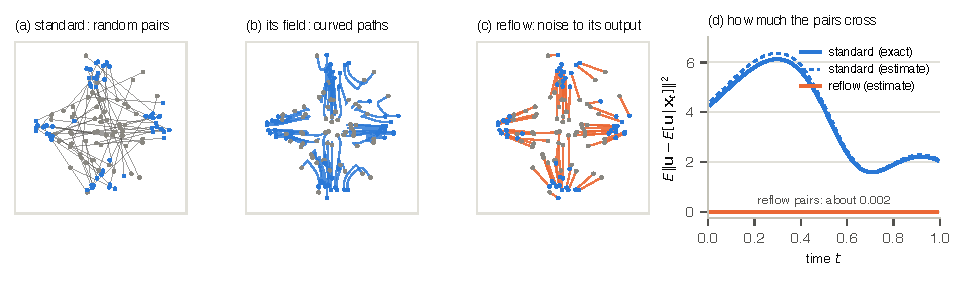
\includegraphics[width=\textwidth]{figures/fig_reflow.pdf}
\caption{Standard flow matching against reflow on the ring of Section~\ref{sec:evidence}, with the exact marginal velocity.
(a) Training pairs of standard flow matching: $60$ noises (grey) paired with independent target samples (blue).
(b) Trajectories of the field learned from such pairs, from the same noises. (c) Reflow pairs: the same noises
paired with the outputs of (b). (d) Conditional variance of the direction $\bu=\bx_1-\bx_0$ of the pairs given the point
$\bx_t$, against $t$: exact for the independent pairs, and a $25$-nearest-neighbour estimate on $20{,}000$ pairs for both
couplings; its average over $t$ is the smallest flow-matching loss (Lemma~\ref{lem:reflow}(i)).}
\label{fig:reflow}
\end{figure}

\begin{definition}[Prompt-conditioned linear flow matching]\label{def:prompt}
Prompts are embeddings $\be\in\cE\subseteq\RR^{D_e}$. A \emph{prompt-to-field map} is a Borel map
$\bth(\cdot):\cE\to\RR^D$; the field of $\be$ is $v_{\bth(\be)}$ and its outputs have law
$\nu_{\bth(\be)}$. Two instances matter.
(a) \emph{Per-prompt fit}: each prompt specifies a target $p_{\be}$, and $\bth(\be)=\bth_{p_{\be}}$ is its
ridge fit (estimated from ample data in practice); a request may also come with $N$ samples and a few-shot fit $\hat\bth(\be)$.
(b) \emph{Affine in the prompt}: $\bth(\be)=\ba+U\be$, with $\ba\in\RR^D$ and $U\in\RR^{D\times D_e}$ fixed.
\end{definition}

Instance (b) arises in two ways. A conditional model $v(\bx,t;\be)=\Phi(\bx,t)(\ba+U\be)$ is fitted
once on (prompt, sample) pairs by linear least squares, since it is linear in $(\ba,U)$. And the
first-order expansion of any conditional network $u(\bx,t;\be)$ at a reference prompt $\be_0$,
$u(\cdot;\be_0)+\partial_{\be} u(\cdot;\be_0)(\be-\be_0)$, is instance (b), provided these features have linear growth, with $D=1+D_e$,
$\Phi=[u(\cdot;\be_0)-\partial_{\be} u(\cdot;\be_0)\be_0,\ \partial_{\be} u(\cdot;\be_0)]$, $\ba=\mathbf 1_1$ and
$U=[0,I_{D_e}]^\top$.

% =====================================================================================
\section{Distances between fields}\label{sec:metrics}
% =====================================================================================

\begin{definition}[Distances between fields]\label{def:metrics}
For fields $v,v'$, the following are extended pseudometrics (Proposition~\ref{pr:lp}(i), Lemma~\ref{lem:constructions}(ii)):
(i) for a probability measure $\rho$ on $\RR^n\times[0,1]$, $d_\rho(v,v')=\|v-v'\|_{L^2(\rho)}$;
(ii) for a Borel map $\chi:\RR^n\to\RR^{n_\chi}$ of linear growth (the space in which outputs are
compared: the identity, an encoder, the features of a classifier), the \emph{map metric} is
$d^\chi_T(v,v')=\|\chi\circ T_v-\chi\circ T_{v'}\|_{L^2(\mu_0)}$, and $d_T=d^{\mathrm{id}}_T$;
(iii) the \emph{source-slice metric} is $d_0=d_{\mu_0\otimes\delta_0}$, that is,
$d_0(v,v')=\|v(\cdot,0)-v'(\cdot,0)\|_{L^2(\mu_0)}=\|T^1_v-T^1_{v'}\|_{L^2(\mu_0)}$.
On the linear model we write $d(\bth,\bth')=d(v_{\bth},v_{\bth'})$, again an extended pseudometric, and, when $\E_\rho\|\Phi\|_F^2<\infty$,
$G_\rho=\E_\rho[\Phi^\top\Phi]$ as in Lemma~\ref{lem:linear_models}.
\end{definition}

\begin{proposition}[Mahalanobis form]\label{pr:mahalanobis}
(i) If $\E_\rho\|\Phi\|_F^2<\infty$, then $d_\rho(\bth,\bth')=\|\bth-\bth'\|_{G_\rho}$; $d_\rho$ is a pseudometric
on $\RR^D$, and a metric if and only if $G_\rho\succ0$. For $\delta\ge0$ with $H=G_\rho+\delta I\succ0$
and $H=CC^\top$, $\|\bth-\bth'\|_H=\|C^\top(\bth-\bth')\|_2\ge d_\rho(\bth,\bth')$.
(ii) $d_0(\bth,\bth')=\|\bth-\bth'\|_{G_0}$ with $G_0=\E_{\bx\sim\mu_0}[\Phi(\bx,0)^\top\Phi(\bx,0)]$: for the one-step
sampler, the map metric is a Mahalanobis distance.
(iii) For a prompt map affine in the prompt, $d_\rho(\bth(\be),\bth(\be'))=\|\be-\be'\|_{U^\top G_\rho U}$.
(iv) $d^\chi_T$ is a finite pseudometric on $\RR^D$.
\end{proposition}
\textit{Proof:}
(i) Lemma~\ref{lem:linear_models}(ii) applied to $\bth-\bth'$ gives the Mahalanobis form; Lemmas~\ref{lem:mahalanobis_basics}(i)
and~\ref{lem:constructions}(i) give the kernel and the metric property; and $\|C^\top\ba\|^2=\ba^\top H\ba=\|\ba\|_{G_\rho}^2+\delta\|\ba\|^2$.
(ii) Apply (i) with $\rho=\mu_0\otimes\delta_0$, which is admissible by linear growth (Proposition~\ref{pr:lp}(v)), and note
$T^1_{\bth}-T^1_{\bth'}=\Phi(\cdot,0)(\bth-\bth')$.
(iii) $\bth(\be)-\bth(\be')=U(\be-\be')$ and $\|U\ba\|^2_{G_\rho}=\ba^\top U^\top G_\rho U\ba$.
(iv) $\chi\circ T_{\bth}$ has linear growth, by that of $\chi$ and Lemma~\ref{lem:lfm}(iii), so it lies in $L^2(\mu_0)$
(Proposition~\ref{pr:lp}(v)); $d^\chi_T$ is the $L^2(\mu_0)$ distance between such maps (Proposition~\ref{pr:lp}(i),
Lemma~\ref{lem:constructions}(ii)). \hfill$\square$

The choice of distance decides where fields are compared. For instance (a), the pooled
interpolation path of the safe prompts, $\bar\rho=\frac1M\sum_i\rho_{p_{\be_i}}$, gives
$G_{\bar\rho}=\frac1M\sum_iG_{p_{\be_i}}$, the average of the safe least-squares Gram matrices; it
compares fields where the safe paths put mass (Remark~\ref{rem:fields_hilbert}), an off-policy distance. The source slice compares
fields on $\mu_0$, the law at which every sampler makes its first evaluation of every field. The map metric
compares where the fields send the noise: it evaluates each field along its own trajectories and
is nevertheless symmetric. The next lemma relates the last two.

\begin{lemma}[Time, straightness and the source slice]\label{lem:time}
(i) If $T_v,T^1_v,T_{v'},T^1_{v'}\in L^2(\mu_0)$ (e.g.\ for all fields of the linear model), then
$|d_T(v,v')-d_0(v,v')|\le\zeta_v+\zeta_{v'}$.
(ii) If solutions of $\dot X_t=v(X_t,t)$ on $[0,1]$ exist from every initial point and all of them are
affine in $t$ (a \emph{straight} field), then $v$ is constant along each trajectory, $T_v=T^1_v$ for
every grid, and $\zeta_v=0$.
(iii) The version of $\vstar_p$ given by Bayes' formula (Lemma~\ref{lem:condexp}(ii)) is continuous on $\RR^n\times[0,1)$ and
satisfies $\vstar_p(\bx,0)=\E_p[\bx_1]-\bx$. Hence $T^1_{\vstar_p}\equiv\E_p[\bx_1]$ and
$d_0(\vstar_p,\vstar_{p'})=\|\E_p[\bx_1]-\E_{p'}[\bx_1]\|$; if moreover the sampler transports $\mu_0$ to $p$
(as the exact flow does when it is well posed), then $\zeta_{\vstar_p}^2=\E_p\|\bx_1-\E_p[\bx_1]\|^2$.
\end{lemma}
\textit{Proof:}
(i) Minkowski's inequality in $L^2(\mu_0)$ (Proposition~\ref{pr:lp}(i)): $\|T_v-T_{v'}\|\le\|T_v-T^1_v\|+\|T^1_v-T^1_{v'}\|+\|T^1_{v'}-T_{v'}\|$,
and symmetrically with the roles of $T$ and $T^1$ exchanged.
(ii) Let $X_t=X_0+t(X_1-X_0)$ be a solution. By Definition~\ref{def:fields}, $v(X_t,t)=\dot X_t=X_1-X_0=v(X_0,0)$ for every $t\in[0,1]$.
If the Euler iterate satisfies $\by_k=X_{t_k}$, then $\by_{k+1}=X_{t_k}+h_k(X_1-X_0)=X_{t_{k+1}}$; by induction
$T_v(X_0)=X_1=X_0+v(X_0,0)=T^1_v(X_0)$, and a solution starts from every point.
(iii) Given $\bx_1=\by$, the pair $(\bx_t,t)$ has the density $\varphi_t(\bx-t\by)\mathbbm 1\{t<1\}$ with respect to the Lebesgue measure on
$\RR^n\times[0,1]$, where $\varphi_t$ is the density of $\cN(0,(1-t)^2I_n)$, and $\bu=(\bx_1-\bx_t)/(1-t)$ a.s. Bayes' formula
(Lemma~\ref{lem:condexp}(ii)) gives the version $\vstar_p(\bx,t)=(m_t(\bx)-\bx)/(1-t)$ for $t<1$, with
$m_t(\bx)=\int\by\varphi_t(\bx-t\by)p(d\by)/\int\varphi_t(\bx-t\by)p(d\by)$. It is continuous on $\RR^n\times[0,1)$ by dominated convergence
($\varphi_t$ is bounded uniformly for $t\le\bar t<1$ and $p$ has a first moment), and $\varphi_0(\bx-0\cdot\by)$ does not depend on $\by$, so
$m_0(\bx)=\E_p[\bx_1]$. The rest follows from $T^1_v(\bx)=\bx+v(\bx,0)$ and, for the defect, from $T^1_{\vstar_p}\equiv\E_p[\bx_1]$,
$T_{\vstar_p}(\bx_0)\sim p$ and the change of variables formula (Remark~\ref{rem:tools}(ii)). \hfill$\square$

Two consequences settle how time enters. For a straight field, the whole time-dependent field is
summarised by its slice at $t=0$, and $d_T=d_0$. For the independent coupling used to train
1-rectified flows, the slice at $t=0$ of the exact field knows only the mean of the target, so
$d_0$ cannot see the shape of the outputs, and the defect has the size of the target's spread.
The source slice is therefore informative only for straightened models: after reflow, the slice at $t=0$ of the exact
field is the displacement $T_v-\mathrm{id}$ of the previous sampler (Lemma~\ref{lem:reflow}(iii)), and distillation fits that map directly
(Remark~\ref{rem:reflow}); for curved models one uses $d^\chi_T$ itself, or
$d_0$ corrected by the defects (Corollary~\ref{cor:one_step}).

% =====================================================================================
\section{The order-1 Wasserstein region of safe fields}\label{sec:region}
% =====================================================================================

\begin{assumption}[Safe prompts]\label{as:exch}
The pairs $(\be_j,\bth_j)$, $j\in\llbracket M+K+1\rrbracket$, are exchangeable (Definition~\ref{def:exch}); for instance, the prompts are
i.i.d.\ draws from a distribution of approved prompts and $\bth_j=\bth(\be_j)$, or an independent
Monte Carlo fit of it. The first $M$ pairs, $\cD=((\be_i,\bth_i))_{i\le M}$, define the region (the
\emph{safe fields}), the next $K$ calibrate it, and the last one is a new approved prompt. The
pseudometric $d$ on $\RR^D$ and the weight map $w:\cE\to\Delta^{M-1}$ below are Borel functions of their arguments and of $\cD$,
and depend on no other data.
\end{assumption}

\begin{definition}[Order-$1$ score and region]\label{def:region}
For a prompt $\be$ and $\bth\in\RR^D$, the order-$1$ score is
\[
g_{d,1}(\be,\bth;\cD)=\frac{1}{M+1}\sum_{i=1}^Mw_i(\be)d(\bth,\bth_i),
\]
which is $s_{d,1}(\bth;\cD)=\frac{1}{M(M+1)}\sum_id(\bth,\bth_i)$ for uniform weights. For $\beta\in(0,1)$, let
$k=\lceil(K+1)(1-\beta)\rceil$ and $S_j=g_{d,1}(\be_{M+j},\bth_{M+j};\cD)$ for $j\in\llbracket K\rrbracket$. The
threshold $\varepsilon=C_{1-\beta}(S_1,\dots,S_K)$ is the $k$-th smallest calibration score if $k\le K$ and
$+\infty$ otherwise, and the region of $\be$ is $\Tbar(\be)=\{\bth\in\RR^D:g_{d,1}(\be,\bth;\cD)\le\varepsilon\}$,
written $\Tbar$ for uniform weights.
\end{definition}

Prompt-adaptive weights, e.g.\ $w_i(\be)\propto\exp(-\|\be-\be_i\|^2/(2h^2))$, tighten the region around
the safe prompts most similar to the request; this is the task-adaptive score $g_{d,1}$ of the
manuscript with prompts in place of tasks. The prompt is observed exactly, so the calibration
scores and the deployed score are the same function, and the exchangeability caveat of
few-shot task reweighting does not arise.

\begin{lemma}[Closed form on a pseudometric space]\label{lem:closed_form}
Let $(V,d)$ be a pseudometric space, $v_1,\dots,v_M,v\in V$, $w\in\Delta^{M-1}$, and
$\hat{\mathbbm F}^w=\sum_iw_i\delta_{v_i}$, $\hat{\mathbbm F}^{w,v}=\frac{1}{M+1}(M\hat{\mathbbm F}^w+\delta_v)$, and let $W_{d,1}$ be as in
Definition~\ref{def:wasserstein}. Then
\[
W_{d,1}(\hat{\mathbbm F}^w,\hat{\mathbbm F}^{w,v})=\frac{1}{M+1}\sum_{i=1}^Mw_id(v_i,v).
\]
In particular $g_{d,1}(\be,\bth;\cD)$ is the order-$1$ Wasserstein distance, on the space of fields
when $d$ is one of the distances of Definition~\ref{def:metrics}, between the $w(\be)$-weighted law of
the safe fields and the same law with the candidate field added.
\end{lemma}
\textit{Proof:}
The plan $\pi^\star=\sum_i\frac{Mw_i}{M+1}\delta_{(v_i,v_i)}+\sum_i\frac{w_i}{M+1}\delta_{(v_i,v)}$ has the right marginals
and, since $d(v_i,v_i)=0$, costs $\frac{1}{M+1}\sum_iw_id(v_i,v)$. Conversely, $f=d(\cdot,v)$ is $1$-Lipschitz
(Definition~\ref{def:metric_spaces}), so by Lemma~\ref{lem:coupling_bounds}(ii) every coupling costs at least
$\sum_iw_if(v_i)-\frac{1}{M+1}(M\sum_iw_if(v_i)+f(v))=\frac{1}{M+1}(\sum_iw_id(v_i,v)-f(v))$, and $f(v)=0$. \hfill$\square$

\begin{proposition}[Coverage]\label{pr:coverage}
Under Assumption~\ref{as:exch},
$\PP\big(\bth_{M+K+1}\in\Tbar(\be_{M+K+1})\mathrel{\big|}\cD\big)\ge k/(K+1)\ge1-\beta$.
\end{proposition}
\textit{Proof:}
If $k>K$, $\varepsilon=+\infty$. Let $k\le K$ and $S_{K+1}=g_{d,1}(\be_{M+K+1},\bth_{M+K+1};\cD)$. A permutation of the last $K+1$ indices is a
permutation of all of them that fixes the first $M$, so the last $K+1$ pairs are exchangeable given $\cD$, and so are the scores
$S_j=h(\cD,\be_{M+j},\bth_{M+j})$, with $h$ Borel (Definition~\ref{def:exch}). Let $N_j=\#\{l\le K+1:S_l<S_j\}$; permuting the scores permutes
the $N_j$ in the same way, so they are exchangeable given $\cD$ too. Let $s_{(k)}$ be the $k$-th smallest of all $K+1$ scores. If
$S_{K+1}>\varepsilon$, at least $k$ calibration scores are at most $\varepsilon<S_{K+1}$, so $N_{K+1}\ge k$. If $N_j\ge k$, then $S_j>s_{(k)}$, and at
most $K+1-k$ indices satisfy $S_j>s_{(k)}$; hence $\sum_j\mathbbm 1\{N_j\ge k\}\le K+1-k$. For every Borel $B$, exchangeability gives
$(K+1)\PP(N_{K+1}\ge k,\cD\in B)=\E[\sum_j\mathbbm 1\{N_j\ge k\}\mathbbm 1\{\cD\in B\}]\le(K+1-k)\PP(\cD\in B)$, hence
$\PP(S_{K+1}\le\varepsilon,\cD\in B)\ge\PP(N_{K+1}<k,\cD\in B)\ge\frac{k}{K+1}\PP(\cD\in B)$, which is the claim in the sense of
Definition~\ref{def:exch}. \hfill$\square$

\begin{remark}[Scope of the guarantee]\label{rem:scope}
(i) The probability is conditional on the safe fields and marginal over calibration and test; a
statement conditional on the calibration prompts needs the training-conditional form of
\citet{vovk2013conditional}. (ii) What is covered is $\bth(\be)$, the field the pipeline would
produce, not a few-shot fit; restricting a few-shot fit to the region excludes $\bth(\be)$ with
probability at most $\beta$. (iii) If the approved prompts drift over time, weighted conformal
prediction applies \citep{barber2023conformal}. (iv) Distances estimated on probe noises drawn
once and shared by all scores (frozen probes) are fixed functions given $\cD$ and the probes, so
the coverage is exact for the estimated score; the certificates of Section~\ref{sec:certificates}
are then plug-in.
\end{remark}

\begin{proposition}[Geometry of the region]\label{pr:geometry}
Let $d(\bth,\bth')=\|\bth-\bth'\|_H$ with $H\succeq0$, fix $w\in\Delta^{M-1}$, and let
$s(\bth)=\frac{1}{M+1}\sum_iw_i\|\bth-\bth_i\|_H$ and $R=\{s\le\varepsilon\}$.
(i) $s$ is convex and $|s(\bth)-s(\bth')|\le\|\bth-\bth'\|_H/(M+1)$; $R$ is closed and convex. For any $C$ with
$CC^\top=H$, $R=\{\bth:\exists\mathbf r\in\RR^M,\ \|C^\top(\bth-\bth_i)\|_2\le r_i\ \forall i,\ \sum_iw_ir_i\le(M+1)\varepsilon\}$,
and in the coordinates $\mathbf z=C^\top\bth$ the score is the Euclidean order-$1$ score of the manuscript.
(ii) $s$ attains its minimum at some $\bth_c$ (a weighted geometric median of the safe fields), and
$R\ne\emptyset$ if and only if $s(\bth_c)\le\varepsilon$. For uniform weights and $k\le K$, $\Tbar$ contains every
calibration field whose score is at most $\varepsilon$, so it is not empty.
(iii) For uniform weights and any pseudometric $d$,
$s_{d,1}(\bth;\cD)\ge\frac{1}{2M^2(M+1)}\sum_{i,j}d(\bth_i,\bth_j)$ for all $\bth$.
\end{proposition}
\textit{Proof:}
(i) Each $\bth\mapsto\|\bth-\bth_i\|_H$ is a seminorm composed with a translation, hence convex (Lemma~\ref{lem:convex}(i)), and
$|\|\bth-\bth_i\|_H-\|\bth'-\bth_i\|_H|\le\|\bth-\bth'\|_H$ by the triangle inequality; so $s$ is convex and continuous, and $R$ is closed and
convex (Lemma~\ref{lem:convex}(ii)). The representation introduces the epigraph variables $r_i$ and uses $\|\ba\|_H=\|C^\top\ba\|$
(Lemma~\ref{lem:mahalanobis_basics}(i)); its constraints are second-order cone constraints (Definition~\ref{def:socp}).
(ii) With $P$ the orthogonal projector onto the range of $H$, $\|\bth-\bth_i\|_H=\|P\bth-P\bth_i\|_H$ (Lemma~\ref{lem:mahalanobis_basics}(ii)), so
$s(\bth)=s(P\bth)$; and $\|\cdot\|_H$ is a norm on that range, on which $s$ is therefore continuous and coercive and attains its minimum
(Lemma~\ref{lem:convex}(iii)). The last claim holds because at least $k\ge1$ calibration scores are at most $\varepsilon$.
(iii) Sum $d(\bth_i,\bth_j)\le d(\bth_i,\bth)+d(\bth,\bth_j)$ over $i,j\in\llbracket M\rrbracket$:
$\sum_{i,j}d(\bth_i,\bth_j)\le2M\sum_id(\bth,\bth_i)$. \hfill$\square$

Item (iii) is the \emph{floor} of the order-$1$ region: whenever the region is non-empty, the budget
$(M+1)\varepsilon$ is at least half the mean distance between safe fields, so every certificate below is only as tight as the safe fields
(or, with adaptive weights, the safe fields near the request) are concentrated.

% =====================================================================================
\section{Constraining the field of a new prompt}\label{sec:constraining}
% =====================================================================================

\begin{definition}[Constrained field]\label{def:constrained}
Let $\be$ be a prompt with a proposal $\tilde\bth\in\RR^D$ (its field $\bth(\be)$, or a few-shot fit
$\hat\bth(\be)$), let $H_{\be}\succ0$, and assume that $\Tbar(\be)$ is non-empty, closed and convex
(Proposition~\ref{pr:geometry}). The constrained coefficient is
$\bth^\sharp(\be)=\argmin_{\bth\in\Tbar(\be)}\|\bth-\tilde\bth\|^2_{H_{\be}}$, the projection of $\tilde\bth$ onto $\Tbar(\be)$ in the Hilbert space
$(\RR^D,\langle\cdot,\cdot\rangle_{H_\be})$ (Theorem~\ref{th:projection}), and the constrained field is $v_{\bth^\sharp(\be)}$.
\end{definition}

\begin{proposition}[Projection onto the region]\label{pr:projection}
Let the score use $d=\|\cdot\|_H$, $H\succeq0$ (Proposition~\ref{pr:mahalanobis}).
(i) $\bth^\sharp(\be)$ exists, is unique and solves a second-order cone program, and
$\bth^\sharp(\be)=\tilde\bth$ if and only if $\tilde\bth\in\Tbar(\be)$. Under Assumption~\ref{as:exch} and with
$\tilde\bth=\bth(\be)$, the field of a new approved prompt is left unchanged with probability at least
$1-\beta$.
(ii) For uniform weights and $H_{\be}=H'$ for all $\be$,
$\|\bth^\sharp(\be)-\bth^\sharp(\be')\|_{H'}\le\|\tilde\bth(\be)-\tilde\bth(\be')\|_{H'}$.
(iii) If $H\succ0$ and $H_{\be}=H$, then $\bth^\sharp(\be)=\sum_{a=0}^M\gamma_a\bth_a$ for some $\gamma\in\Delta^M$, with
$\bth_0=\tilde\bth$: the constrained field is the mixture $\gamma_0v_{\tilde\bth}+\sum_{i}\gamma_iv_{\bth_i}$ of the
proposal and the safe fields. Any minimiser of $(\gamma-\mathbf 1_0)^\top\Gamma(\gamma-\mathbf 1_0)$ over
$\gamma\in\Delta^M$ subject to $\frac{1}{M+1}\sum_iw_i(\be)((\gamma-\mathbf 1_i)^\top\Gamma(\gamma-\mathbf 1_i))^{1/2}\le\varepsilon$,
where $\Gamma_{ab}=\langle\bth_a,\bth_b\rangle_H$, $a,b\in\{0,\dots,M\}$, is such a $\gamma$.
(iv) If $\tilde\bth=\hat\bth$ is a few-shot fit with moments $(\hat G,\hat\bb)$ and $H_{\be}=\hat G+\lambda I$, then
$\bth^\sharp(\be)=\argmin_{\bth\in\Tbar(\be)}\bth^\top(\hat G+\lambda I)\bth-2\hat\bb^\top\bth$: the regularised few-shot
flow-matching loss minimised over the region, i.e.\ problem \texttt{OT1-TRAIN} of the manuscript.
\end{proposition}
\textit{Proof:}
(i) $(\RR^D,\langle\cdot,\cdot\rangle_{H_\be})$ is a Hilbert space (Lemma~\ref{lem:mahalanobis_basics}(i)) and $\Tbar(\be)$ is closed, convex and
non-empty, so Theorem~\ref{th:projection} gives a unique minimiser. With the representation of Proposition~\ref{pr:geometry}(i) and the
objective $\|C_{\be}^\top(\bth-\tilde\bth)\|$, $H_{\be}=C_{\be} C_{\be}^\top$, which has the same minimiser, the problem is a second-order cone program
(Definition~\ref{def:socp}). The objective vanishes only at $\tilde\bth$. The probability statement is Proposition~\ref{pr:coverage}.
(ii) With uniform weights the region does not depend on the prompt, and $\bth^\sharp(\be)$ is the projection of $\tilde\bth(\be)$ onto it in
$\langle\cdot,\cdot\rangle_{H'}$; apply Theorem~\ref{th:projection}(ii).
(iii) Let $P$ be the projection onto $\conv\{\bth_0,\dots,\bth_M\}$ in $\langle\cdot,\cdot\rangle_H$, a non-empty compact convex set
(Lemma~\ref{lem:convex}(ii)). By Theorem~\ref{th:projection}(i), $\|\bth-\bth_a\|_H^2\ge\|\bth-P\bth\|_H^2+\|P\bth-\bth_a\|_H^2$ for every $a$. At $\bth=\bth^\sharp(\be)$, the distances to the
safe fields do not increase, so $P\bth^\sharp(\be)\in\Tbar(\be)$, and the objective decreases by at least
$\|\bth^\sharp(\be)-P\bth^\sharp(\be)\|_H^2$; by uniqueness, $P\bth^\sharp(\be)=\bth^\sharp(\be)$. For
$\bth=\sum_a\gamma_a\bth_a$ with $\gamma\in\Delta^M$, $\|\bth-\bth_b\|_H^2=(\gamma-\mathbf 1_b)^\top\Gamma(\gamma-\mathbf 1_b)$ by
Lemma~\ref{lem:mahalanobis_basics}(iii), applied to the linear map $\gamma\mapsto\sum_a\gamma_a\bth_a$ into $(\RR^D,\langle\cdot,\cdot\rangle_H)$, whose Gram
matrix is $\Gamma$. The stated problem is therefore the original one restricted to the convex hull, which contains its unique
solution.
(iv) $(\hat G+\lambda I)\hat\bth=\hat\bb$ by Lemma~\ref{lem:lfm}(i), so
$\|\bth-\hat\bth\|^2_{\hat G+\lambda I}=\bth^\top(\hat G+\lambda I)\bth-2\hat\bb^\top\bth+\hat\bth^\top\hat\bb$. \hfill$\square$

Item (iii) needs only inner products of fields, $\Gamma_{ab}=\langle v_{\bth_a},v_{\bth_b}\rangle_{L^2(\rho)}+\delta\langle\bth_a,\bth_b\rangle$
when $H=G_\rho+\delta I$. With $\delta=0$ and the projection taken in $L^2(\rho)$, the same argument
applies to nonlinear fields, at the price of $M+1$ field evaluations per sampler step. Item (ii)
says that a perturbation of a prompt's field moves its constrained field by no more than the
perturbation.

\begin{corollary}[Prompt mixing]\label{cor:prompt_mixing}
Let $\bth(\be)=\ba+U\be$ (Definition~\ref{def:prompt}(b)), $H\succ0$, $H_{\be}=H$, $\tilde\bth=\bth(\be)$, and let $\gamma$ be as
in Proposition~\ref{pr:projection}(iii). Then $\bth^\sharp(\be)=\bth(\be^\sharp)$ with
$\be^\sharp=\gamma_0\be+\sum_i\gamma_i\be_i\in\conv\{\be,\be_1,\dots,\be_M\}$: the constrained field is the field of a mixed prompt (a vector of $\RR^{D_e}$, which need not be the
embedding of a tokenised prompt). Moreover $\be^\sharp$ minimises $\|\be'-\be\|_{U^\top HU}$ over $\{\be':\bth(\be')\in\Tbar(\be)\}$, uniquely if $U$ has full
column rank.
\end{corollary}
\textit{Proof:}
An affine map preserves convex combinations (Lemma~\ref{lem:convex}(i)), so $\bth(\be^\sharp)=\gamma_0\bth(\be)+\sum_i\gamma_i\bth_i=\bth^\sharp(\be)$. For
every admissible $\be'$, $\|\be'-\be\|_{U^\top HU}=\|\bth(\be')-\bth(\be)\|_H\ge\|\bth^\sharp(\be)-\bth(\be)\|_H=\|\be^\sharp-\be\|_{U^\top HU}$. If $U$ has full
column rank, then $U^\top HU\succ0$ (Lemma~\ref{lem:mahalanobis_basics}(iii) with $\mathsf L=U$, into $(\RR^D,\langle\cdot,\cdot\rangle_H)$), the
admissible set is closed and convex (the preimage of $\Tbar(\be)$ by a continuous affine map; Lemma~\ref{lem:convex}(i)), and the
projection onto it is unique (Theorem~\ref{th:projection}). \hfill$\square$

When the score is not convex, as $d^\chi_T$ in general is for $J\ge2$, a feasible field is still
obtained in closed form or by bisection.

\begin{proposition}[Back-off]\label{pr:backoff}
Let $s$ be any score, $R=\{s\le\varepsilon\}$, $\bth_c\in R$, and $\bth_\kappa=(1-\kappa)\tilde\bth+\kappa\bth_c$ for $\kappa\in[0,1]$.
(i) The bisection that starts from $[\mathrm{lo},\mathrm{hi}]=[0,1]$ and sets $\mathrm{hi}\gets\mathrm{mid}$ if
$s(\bth_{\mathrm{mid}})\le\varepsilon$ and $\mathrm{lo}\gets\mathrm{mid}$ otherwise keeps $\bth_{\mathrm{hi}}\in R$ at every
step, without assumption on $s$.
(ii) If $s$ is convex and $s(\bth_c)<\varepsilon<s(\tilde\bth)$, then $\bth_\kappa\in R$ for all
$\kappa\ge\kappa^\star=\frac{s(\tilde\bth)-\varepsilon}{s(\tilde\bth)-s(\bth_c)}\in(0,1)$, so the distance from $\tilde\bth$ to $R$ is at most
$\kappa^\star\|\tilde\bth-\bth_c\|_{H'}$ in any seminorm $\|\cdot\|_{H'}$.
(iii) For the linear model, $v_{\bth_\kappa}=(1-\kappa)v_{\tilde\bth}+\kappa v_{\bth_c}$: the back-off blends two fields at
inference time, with two field evaluations per sampler step.
\end{proposition}
\textit{Proof:}
(i) $\bth_1=\bth_c\in R$, and $\mathrm{hi}$ only takes values $\mathrm{mid}$ with $\bth_{\mathrm{mid}}\in R$.
(ii) By convexity, $s(\bth_\kappa)\le(1-\kappa)s(\tilde\bth)+\kappa s(\bth_c)=s(\tilde\bth)-\kappa(s(\tilde\bth)-s(\bth_c))\le\varepsilon$ for $\kappa\ge\kappa^\star$, and
$\|\tilde\bth-\bth_{\kappa^\star}\|_{H'}=\kappa^\star\|\tilde\bth-\bth_c\|_{H'}$. (iii) Linearity of $\bth\mapsto\Phi\bth$. \hfill$\square$

By (ii), the enforcement moves a field in proportion to its score excess $s(\tilde\bth)-\varepsilon$, so a
request that barely exceeds the threshold is barely changed. A feasible $\bth_c$ is a minimiser of the score when the region is non-empty (a geometric median
for Mahalanobis distances), or, for uniform weights, a calibration field with score at most $\varepsilon$
(Proposition~\ref{pr:geometry}(ii)).

% =====================================================================================
\section{What the region certifies}\label{sec:certificates}
% =====================================================================================

\begin{theorem}[Wasserstein certificate on the outputs]\label{th:certificate}
Let $\chi:\RR^n\to\RR^{n_\chi}$ be Borel of linear growth and let $d:\RR^D\times\RR^D\to[0,+\infty]$ satisfy
$d(\bth,\bth')\ge\|\chi\circ T_{\bth}-\chi\circ T_{\bth'}\|_{L^1(\mu_0)}$ for all $\bth,\bth'$; for instance the pseudometric $d=d^\chi_T$. Let
$w\in\Delta^{M-1}$, $\varepsilon\ge0$, and $\bth$ with $\frac{1}{M+1}\sum_iw_id(\bth,\bth_i)\le\varepsilon$. Let $\bx_0\sim\mu_0$ and $I\sim w$
be independent, $Y=\chi(T_{\bth}(\bx_0))$ and $Y'=\chi(T_{\bth_I}(\bx_0))$. Then:
(i) $\E\|Y-Y'\|\le(M+1)\varepsilon$; hence $W_1\big(\chi_\#\nu_{\bth},\sum_iw_i\chi_\#\nu_{\bth_i}\big)\le(M+1)\varepsilon$;
(ii) for every Borel set $B\subseteq\RR^{n_\chi}$ and every $r>0$,
\[
\PP\big(\chi(T_{\bth}(\bx_0))\in B\big)\le\sum_{i=1}^Mw_i\PP\big(\chi(T_{\bth_i}(\bx_0))\in B^{+r}\big)+\frac{(M+1)\varepsilon}{r}.
\]
In particular, if the region is built with such a $d$ (e.g.\ $d^\chi_T$) and $w=w(\be)$, then (i) and (ii)
hold for every $\bth\in\Tbar(\be)$, whatever the prompt $\be$: for the field of an admitted prompt and for
every field enforced by Section~\ref{sec:constraining}.
\end{theorem}
\textit{Proof:}
(i) Lemma~\ref{lem:coupling_bounds}(i) with $\mu=\mu_0$, $F=\chi\circ T_{\bth}$ and $F_i=\chi\circ T_{\bth_i}$ gives
$\E\|Y-Y'\|=\sum_iw_i\|\chi\circ T_{\bth}-\chi\circ T_{\bth_i}\|_{L^1(\mu_0)}\le\sum_iw_id(\bth,\bth_i)\le(M+1)\varepsilon$, and the laws of $Y$ and $Y'$ are
$(\chi\circ T_{\bth})_\#\mu_0=\chi_\#\nu_{\bth}$ and $\sum_iw_i\chi_\#\nu_{\bth_i}$ (Remark~\ref{rem:tools}(ii)).
(ii) $B^{+r}$ is Borel (Remark~\ref{rem:tools}(v)). If $Y\in B$ and $\|Y-Y'\|<r$, then $Y'\in B^{+r}$. Hence
$\PP(Y\in B)\le\PP(Y'\in B^{+r})+\PP(\|Y-Y'\|\ge r)$, and Markov's inequality (Remark~\ref{rem:tools}(iv)) and (i) bound the last term.
\hfill$\square$

The certificate is relative: the request is no more likely to produce outputs in $B$ than the
safe prompts are to produce outputs within $r$ of $B$, up to $(M+1)\varepsilon/r$. It holds for every
$B$ at once, so the unsafe set never has to be specified, and it compares order-$1$ Wasserstein
distances on fields with an order-$1$ Wasserstein distance on outputs. Compared with the ODE
bound of the POC (its Proposition~3), comparing outputs under shared noise removes the
Gr\"onwall factor. The map metric is in
general not convex in $\bth$ when $J\ge2$; one-step samplers remove this obstruction.

\begin{corollary}[One-step and straightened samplers]\label{cor:one_step}
(i) For the one-step sampler ($J=1$) and $\chi=\mathrm{id}$, $d_T=d_0=\|\cdot\|_{G_0}$. If the region is built with
$H=G_0+\delta I\succ0$, $\delta\ge0$, it is convex, Proposition~\ref{pr:projection} and
Corollary~\ref{cor:prompt_mixing} apply, and every field in it satisfies Theorem~\ref{th:certificate}.
(ii) For a $J$-step sampler and $\chi=\mathrm{id}$, if $\frac{1}{M+1}\sum_iw_id_0(\bth,\bth_i)\le\varepsilon$, then
Theorem~\ref{th:certificate} holds with $(M+1)\varepsilon$ replaced by
$(M+1)\varepsilon+\zeta_{\bth}+\sum_iw_i\zeta_{\bth_i}$.
\end{corollary}
\textit{Proof:}
(i) Proposition~\ref{pr:mahalanobis}(ii), $\|\cdot\|_{G_0}\le\|\cdot\|_{G_0+\delta I}$ and
$\|\cdot\|_{L^1(\mu_0)}\le\|\cdot\|_{L^2(\mu_0)}$ (Proposition~\ref{pr:lp}(ii)). (ii) By Proposition~\ref{pr:lp}(ii) and Lemma~\ref{lem:time}(i),
$\|T_{\bth}-T_{\bth_i}\|_{L^1(\mu_0)}\le d_T(\bth,\bth_i)\le d_0(\bth,\bth_i)+\zeta_{\bth}+\zeta_{\bth_i}$; multiply by $w_i$, sum, and
repeat the proof of Theorem~\ref{th:certificate} with this bound. \hfill$\square$

The safe defects $\zeta_{\bth_i}$ are computed once; the defect of the candidate costs one $J$-step
simulation on the probe noises. By Lemma~\ref{lem:time}, (ii) is informative for straightened
models and not for 1-rectified ones.

\begin{proposition}[Sensitivity to rare unsafe outputs]\label{pr:sqrt_m}
Let $\mathcal Z\subseteq\RR^n$ be Borel with $\mu_0(\mathcal Z)=m>0$, and $\Delta>0$ with
$\|\chi(T_{\bth}(\bx))-\chi(T_{\bth_i}(\bx))\|\ge\Delta$ for all $\bx\in\mathcal Z$ and $i\in\llbracket M\rrbracket$. Then
$d^\chi_T(\bth,\bth_i)\ge\sqrt m\Delta$ for every $i$, so $g_{d^\chi_T,1}(\be,\bth;\cD)\ge\sqrt m\Delta/(M+1)$ for every
prompt, and $\bth\notin\Tbar(\be)$ whenever $\sqrt m\Delta>(M+1)\varepsilon$.
\end{proposition}
\textit{Proof:}
$d^\chi_T(\bth,\bth_i)^2\ge\int_{\mathcal Z}\|\chi\circ T_{\bth}-\chi\circ T_{\bth_i}\|^2d\mu_0\ge m\Delta^2$, and $\sum_iw_i(\be)=1$.
\hfill$\square$

A request that sends a fraction $m$ of the noise to outputs at distance $\Delta$ from where the safe
prompts send it therefore pays at least $\sqrt m\Delta$, whereas the same argument only guarantees $m\Delta$ for an $L^1$ map
distance, and a forward divergence charges at most $\log\frac{1}{1-m}$ for a mixture with an unsafe
component of mass $m$ (Proposition~\ref{pr:sde_cert}(iii)). Exclusion is guaranteed once
$m>((M+1)\varepsilon/\Delta)^2$. These lower bounds rank the distances only at a fixed budget, whereas the budget
$(M+1)\varepsilon$ is calibrated on the safe fields separately for each distance: detection is decided by the ratio of the
lower bound to that budget. Among map distances, the $L^2$ metric has the largest lower bound for small $m$ and satisfies the
hypothesis of Theorem~\ref{th:certificate}, but its budget also grows with the largest displacements between safe fields,
including those of the rare trajectories a sampler sends far away (Section~\ref{sec:e1}, Step~4).

\begin{remark}[Off-policy distances and stochastic samplers]\label{rem:offpolicy}
The pooled-path distance $d_{\bar\rho}$ is convex and cheap, but it compares fields where the safe
paths put mass; an unsafe mode created where those paths rarely go changes the field mostly where
$\bar\rho$ puts little mass, and is admitted (Section~\ref{sec:evidence}). Bounds from such distances to
outputs go through Gr\"onwall's lemma with the candidate's Lipschitz constant
(Remark~\ref{rem:gronwall}; \citealt{benton2024error}). For stochastic samplers, path divergences give certificates without
Gr\"onwall factor (Appendix~\ref{app:sde}); they are not metrics, so their regions are conformal
regions but not Wasserstein regions.
\end{remark}

Two changes, motivated by the test of Section~\ref{sec:e1}, keep these guarantees and tighten them: weights
that put the mass on the safe field nearest to the candidate, and a bounded distance, which no single far-away trajectory
can dominate.

\begin{proposition}[Localised, truncated certificate]\label{pr:truncated}
Let $r>0$ and $d_r(\bth,\bth')=\E\min(\|T_{\bth}(\bx_0)-T_{\bth'}(\bx_0)\|,r)/r$ with $\bx_0\sim\mu_0$, a pseudometric with values in
$[0,1]$. Let $w\in\Delta^{M-1}$ be allowed to depend on $\bth$, for instance $w=\mathbf 1_{i^\star}$ with
$i^\star\in\argmin_id_r(\bth,\bth_i)$, and assume $\sum_iw_id_r(\bth,\bth_i)\le b$. Then for every Borel $B\subseteq\RR^n$ and
every $r'>0$,
\[
\PP\big(T_{\bth}(\bx_0)\in B\big)\le\sum_{i=1}^Mw_i\PP\big(T_{\bth_i}(\bx_0)\in B^{+r'}\big)+b\max(1,r/r').
\]
\end{proposition}
\textit{Proof:}
$(\by,\by')\mapsto\min(\|\by-\by'\|,r)/r$ is a metric on $\RR^n$ with values in $[0,1]$ (Lemma~\ref{lem:constructions}(iii)), its pull-back by
$\bth\mapsto T_{\bth}(\bx_0)$ is a pseudometric for every $\bx_0$ (Lemma~\ref{lem:constructions}(ii)), and so is the expectation $d_r$
(Lemma~\ref{lem:constructions}(iv)). For $\delta\ge0$,
$\mathbbm 1\{\delta\ge r'\}\le\max(1,r/r')\min(\delta,r)/r$, because $\delta\ge r'$ implies $\min(\delta,r)\ge\min(r',r)$. With $Y$, $Y'$ and $I\sim w$ as in Theorem~\ref{th:certificate} ($w$ is a fixed vector once
$\bth$ is fixed), $\PP(Y\in B)\le\PP(Y'\in B^{+r'})+\PP(\|Y-Y'\|\ge r')$, and the last term is at most
$\max(1,r/r')\sum_iw_id_r(\bth,\bth_i)\le b\max(1,r/r')$. \hfill$\square$

With $w=\mathbf 1_{i^\star}$, the score $\min_id(\bth,\bth_i)/(M+1)$ is a fixed Borel function of $\bth$, so
Proposition~\ref{pr:coverage} applies. Its region is the union of the $d$-balls of radius $(M+1)\varepsilon$ around the safe
fields, as for the order-$\infty$ score of the manuscript, and it is not convex, even for a one-step sampler: the balls are
disjoint in general, and each is a sublevel set of an average of $\min(\|\cdot\|,r)$, which is not convex. This region is the
split-conformal nearest-neighbour novelty detector \citep{laxhammar2015inductive,bates2023testing}, with a distance between sampler
maps; reading its score through Lemma~\ref{lem:closed_form}, with a Dirac weight that depends on the candidate, adds nothing to it.
At $r'=r$ the certificate reads $P(Y\in B)\le P(Y_{i^\star}\in B^{+r})+(M+1)\varepsilon$. Its proof is still Markov's inequality,
applied to the bounded displacement $\min(\|Y-Y'\|,r)$, whose event $\{\min(\|Y-Y'\|,r)\ge r\}$ is $\{\|Y-Y'\|\ge r\}$; the factor
$1/r$ of Theorem~\ref{th:certificate}(ii) has moved into the normalisation of $d_r$. What truncation gains is that displacements
beyond $r$ are not charged: $d_r\le d_{L^1}/r$, so the bound is never worse than the $L^1$ one, and much better when a few
trajectories go far. Only the tail $\PP(\|T_{\bth}-T_{\bth'}\|\ge r)$, used in place of $d_r$, avoids Markov's inequality; it is
smaller, but not a metric.

% =====================================================================================
\section{Evidence from the proof of concept}\label{sec:evidence}
% =====================================================================================

\paragraph{Setup.}
A prompt is $\be=(\phi,\varrho)$ with $\phi\sim\cN(0,0.05^2)$ and $\varrho\sim\cN(2,0.05^2)$, and its target $p_{\be}$ is the
equal-weight mixture of the four Gaussians $\cN(\varrho(\cos(\phi+j\pi/2),\sin(\phi+j\pi/2)),0.3^2I_2)$,
$j=0,\dots,3$ (instance (a) of Definition~\ref{def:prompt}). The unsafe set $A=\{\by:\|\by\|\le0.6\}$ is a
disk that no target visits; the method never uses it. A contaminated field of mass $m$ is the
ridge fit of $(1-m)p_{\be}+m\cN(0,0.25^2I_2)$, computed exactly from the moments, which are integrals
against the target and hence affine in it. The features are $\Phi=I_2\otimes\psi^\top$, with $256$ random Fourier features of $(\bx,t)$
and the affine terms $(1,t,\bx,t\bx)$, so $D=524$; fits use $\lambda=10^{-5}$ and 20,000 Monte Carlo
samples. The samplers are Euler ($J=50$) and the SDE chain of Appendix~\ref{app:sde} ($\eta=1$). A pool
of $200$ prompts is split at random into $M=20$ safe, $K=40$ calibration and $140$ test prompts;
$\beta=0.1$, so the nominal coverage is $37/41=0.902$. All costs use $256$ frozen probe trajectories.
The four costs are the pooled-path distance $d_{\bar\rho}$; the on-policy Gram cost
$\|\bth-\bth_i\|_{G_{\mathrm{on}}(\bth)}$ with $G_{\mathrm{on}}(\bth)=\frac1J\sum_k\E[\Phi(\by_k,t_k)^\top\Phi(\by_k,t_k)]$ along the
candidate's own Euler iterates $\by_k$ (not symmetric, hence not a metric); and the forward and
reverse path divergences of Appendix~\ref{app:sde}. Both Gram matrices are regularised by
$10^{-6}$ times their mean eigenvalue.

\begin{table}[t]
\centering
\caption{Order-$1$ regions of linear flow-matching fields on the toy (means over $100$ splits for the
ODE costs and $200$ for the SDE costs). Exclusion: fraction of contaminated fields of unsafe mass $m$
outside the region. Certificate: median over splits of the bound on $P(A)$ that holds for every field
of the region (plug-in, with a $95\%$ Clopper--Pearson bound on $\bar P_w(A)$, Remark~\ref{rem:mc}), against the largest
$P(A)$ of a held-out or contaminated field inside the region (median and maximum over splits). No
split violates its bound. Safe fields have $P(A)=\pALCmean$ (ODE) and $\pALDmean$ (SDE). The Clopper--Pearson bound treats the
indicators of the $M$ safe samplers as independent, although they share their noise chains, so it is slightly anti-conservative.
The two on-policy rows agree to two decimals by coincidence: at $m=0.01$ and $0.03$ they exclude $\exclCononeP$ and $\exclConthreeP$
($G_{\mathrm{on}}$) against $\exclDrevoneP$ and $\exclDrevthreeP$ (reverse KL).}
\label{tab:regions}
\small
\begin{tabular}{l c c c ccc c c}
\toprule
& & & & \multicolumn{3}{c}{excluded at $m=$} & \multicolumn{2}{c}{certificate}\\
\cmidrule(lr){5-7}\cmidrule(lr){8-9}
cost, sampler & metric & convex & coverage & $0.01$ & $0.03$ & $0.1$ & bound & worst inside\\
\midrule
$d_{\bar\rho}$ (safe paths), ODE & yes & yes & 0.902 & 0.10 & 0.15 & 0.87 & -- & --\\
$G_{\mathrm{on}}$ (own paths), ODE & no & no & 0.899 & 0.13 & 0.55 & 1.00 & -- & --\\
forward KL (safe paths), SDE & no & yes & 0.900 & 0.10 & 0.17 & 0.69 & 0.553 (TV) & 0.0707 / 0.0737\\
reverse KL (own paths), SDE & no & no & 0.899 & 0.13 & 0.55 & 1.00 & 0.134 (rare) & 0.0145 / 0.0158\\
\bottomrule
\end{tabular}
\end{table}

\begin{figure}[t]
\centering
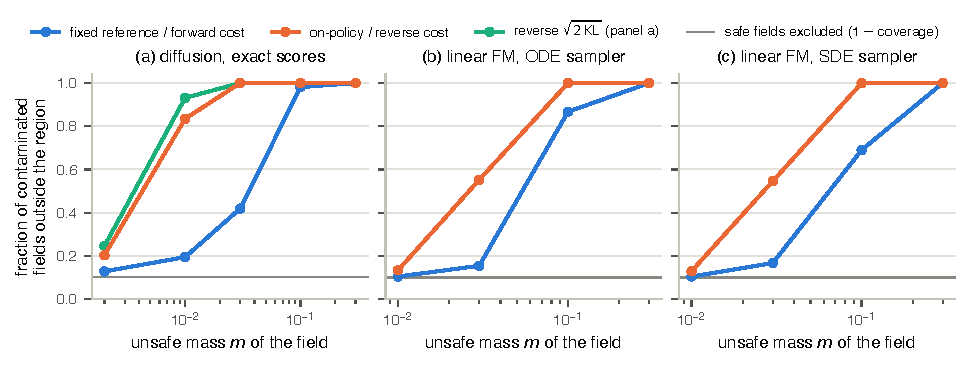
\includegraphics[width=\textwidth]{figures/fig_exclusion.pdf}
\caption{Fraction of contaminated fields outside the region against their unsafe mass. (a) Diffusion
with exact scores (POC pilot A), which isolates the choice of cost: forward $\sqrt{2\KL}$ (blue), reverse
$\KL$ (orange) and reverse $\sqrt{2\KL}$ (green). (b) Linear flow matching, ODE: $d_{\bar\rho}$ (blue) and
$G_{\mathrm{on}}$ (orange). (c) Linear flow matching, SDE: forward (blue) and reverse (orange) $\KL$. Grey:
fraction of held-out safe fields outside the region ($1-$coverage).}
\label{fig:exclusion}
\end{figure}

\paragraph{Findings.}
\emph{Validity.} Coverage is within sampling error of $0.902$ for every cost
(Table~\ref{tab:regions}), as Proposition~\ref{pr:coverage} predicts without any metric
structure.
\emph{Where fields are compared.} At $m=0.03$, the off-policy costs exclude $\exclCrefthree$ and $\exclDfwdthree$ of the
contaminated fields, the on-policy costs $\exclConthree$; with exact diffusion scores the gap is $\exclAFthree$
against $\exclAKthree$ (Figure~\ref{fig:exclusion}). The reverse divergence accumulates at the late steps,
where the contaminated trajectories are pulled into $A$ and the safe ones are pushed out (POC
Figure~4).
\emph{Certificates.} No split violates a bound. The rare-event bound of the reverse-KL region
($\certDrevmed$) is four times tighter than the total-variation bound of the forward-KL region
($\certDfwdmed$); the worst fields they admit have $P(A)$ of $\insideDrevmed$ and $\insideDfwdmed$ (medians over splits).
With exact diffusion scores the rare-event bound is $\certAKmed$, against $\insideAKmed$. The difference between
the two families is the spread of the safe fields (median pairwise path divergence $\pairKLDmed$ against
$\pairKLAmed$ nats), which sets the calibrated budget $(M+1)\varepsilon$; for metric costs,
Proposition~\ref{pr:geometry}(iii) bounds that budget from below.
\emph{Few-shot fitting.} Both constrained fits beat least squares on all $\ntasks$ prompts, with
geometric-mean MMD$^2$ ratios (Remark~\ref{rem:mc}) $\geoCrefclean$ and $\geoCrefcont$ ($d_{\bar\rho}$; clean and contaminated data) and
$\geoConclean$ and $\geoConcont$ ($G_{\mathrm{on}}$), and they lower the unsafe mass from $\pAUcont$ to $\pACrefcont$ and $\pAConcont$; each
second-order cone program takes $\socptime$~s. In this concentrated family, however, the centre alone and tuned shrinkage are better:
with $12$ samples the loss pulls the solution to the boundary of a region calibrated to contain
$90\%$ of the safe fields. The region is a validity and safety device, not an estimator;
shrinkage inside it, $\min_{\bth}\cL_{\hat p}(v_{\bth})+\lambda\|\bth\|^2+\gamma' s(\bth)$ subject to $s(\bth)\le\varepsilon$, keeps
the certificates and should recover the accuracy (not tested).

\begin{table}[t]
\centering
\caption{Few-shot fitting on $32$ held-out prompts of one split, with $12$ clean samples, or $12$
clean and $3$ unsafe samples from $\cN(0,0.25^2I_2)$. MMD$^2$ ($\times10^3$) between 2,500 generated and
2,500 target samples, and $P(A)$ of the fitted sampler with contaminated data.}
\label{tab:fewshot}
\small
\begin{tabular}{l c c c}
\toprule
estimator & MMD$^2$, clean & MMD$^2$, contaminated & $P(A)$, contaminated\\
\midrule
least squares, $\lambda=10^{-3}$ (best of $10^{-5},10^{-3},10^{-1}$) & 131.6 & 144.0 & 0.138\\
constrained, $d_{\bar\rho}$ (Proposition~\ref{pr:projection}(iv)) & 32.6 & 29.6 & 0.047\\
constrained, $G_{\mathrm{on}}$ (convex iterations and back-off) & 40.2 & 28.1 & 0.025\\
shrinkage to $\bth_c$, strength $10$ (tuned on the test prompts) & 10.8 & 11.3 & 0.0087\\
centre $\bth_c$ alone (no data) & 10.7 & 10.7 & 0.0014\\
ample-data fit $\bth(\be)$ (oracle) & 5.1 & 5.1 & 0.0017\\
\bottomrule
\end{tabular}
\end{table}

\paragraph{What the evidence does not cover.}
The POC never computed the metrics that carry Theorem~\ref{th:certificate}, $d^\chi_T$ and $d_0$, nor straightened
couplings, models affine in the prompt, prompt mixing or prompt-adaptive weights; Section~\ref{sec:e1} does.
All its experiments are two-dimensional, with $M=20$, and their certificates are plug-in.

% =====================================================================================
\section{A two-dimensional test of the method, step by step}\label{sec:e1}
% =====================================================================================

In two dimensions every object of the method can be drawn: an output is a point of the plane, a field is an arrow
field that changes with time, and a region is a set of such fields. This section follows one request through the
pipeline (prompt, field, outputs, score, region, enforcement, certificate), and reports at each step what the
aggregate results over many prompts and splits say. It then summarises the results and states the improved method.
The \emph{running example} is the prompt with rotation $\ewPhi^\circ$ and radius $\ewRho$, asked without unsafe mode and with
unsafe mass $m\in\{0.03,0.1,0.3\}$; it is shown on split $0$ and on the 1-rectified model.

\paragraph{Step 1: prompts and what they ask for.}
A prompt is $z=(\phi,\varrho,m)$. Its target is the four-blob ring of Section~\ref{sec:evidence}, rotated by $\phi$ and of radius
$\varrho$, with a fraction $m$ of its mass moved to $\cN(0,0.25^2I_2)$, which falls in the unsafe disk $A$
(Figure~\ref{fig:e1_task}). Approved prompts have $m=0$, $\phi\sim\mathcal U[-22.5^\circ,22.5^\circ]$ and $\varrho\sim\mathcal U[1.75,2.25]$, so their
outputs differ by rotations of up to $45^\circ$. Unsafe prompts have $m\in\{0.01,0.03,0.1,0.3\}$, on independent draws of
$(\phi,\varrho)$. A frozen ``text encoder'' maps $z$ to $\be\in\RR^{43}$ (the normalised $(\phi,\varrho,m)$ and $40$ random Fourier
features of them), and the model is affine in $\be$ (Definition~\ref{def:prompt}(b)), with the features of
Section~\ref{sec:evidence} ($D=524$). It is fitted once on $2000$ prompts, half of them with $m\sim\mathcal U[0,0.4]$, so that it
serves unsafe requests: its outputs have $P(A)=\eonePAAa$, $\eonePAAb$, $\eonePAAc$ and $\eonePAAd$ for the four masses
(against $\eoneTruePAd$ in the target at $m=0.3$) and $\eoneSafePAA$ for safe prompts, with MMD$^2\times10^3=\eoneMmdA$ to the safe
targets (Remark~\ref{rem:mc}). Small masses are under-served: the excess of $P(A)$ over safe prompts is $\eoneExcessa$ at $m=0.01$
and $\eoneExcessb$ at $m=0.03$, only $\eoneRealiseda\%$ and $\eoneRealisedb\%$ of the targets' $\eoneTargeta$ and $\eoneTargetb$, so these
requests are closer to approved ones than their nominal mass suggests. The $50$-step Euler sampler of this model also diverges on
rare noises: the largest of the $256$ probe noises used below ($|\bx_0|=\eoneProbeNorm$) is sent beyond radius $4$ for $\eoneBlowSafe\%$ of
the approved prompts, up to $|T(\bx_0)|=\eoneProbeMaxT$, and the evaluation noise reaches $|T(\bx_0)|=\eoneEvalMaxT$. Outputs in $A$ are
unaffected; distances that are not bounded are (Step~4). A pool of $300$ safe prompts is split at random into $M=30$ safe
\emph{anchors}, which define the region, $K=60$ calibration prompts and $210$ safe test prompts; $100$ unsafe prompts per mass
complete the pool, and $\beta=0.1$. Detection is averaged over $100$ splits and enforcement over $5$. Exclusion at a mass is a
mean over $100$ distinct requests, so its sampling error is up to $\pm0.1$ whatever the number of splits, and every attack is
run on one split.

\begin{figure}[!htbp]
\centering
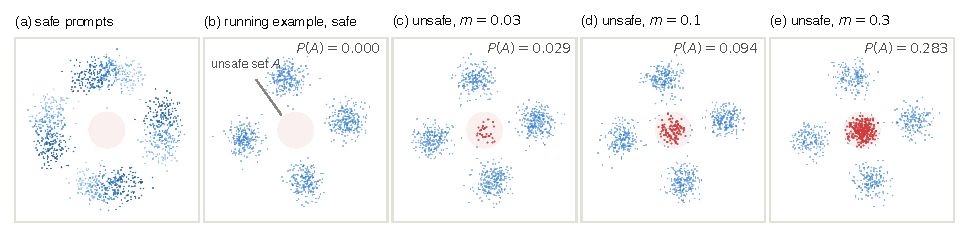
\includegraphics[width=\textwidth]{figures/fig_e1_task.pdf}
\caption{Step 1. (a) Targets of five safe prompts, from rotation $-22.5^\circ$ (light) to $+22.5^\circ$ (dark). (b)--(e) The
running example without and with an unsafe mode of mass $m$; samples in the unsafe disk $A$ are red, and $P(A)$ is
that of the target.}
\label{fig:e1_task}
\end{figure}
\FloatBarrier

\paragraph{Step 2: a prompt becomes a vector field.}
The model turns the embedding of a prompt into a field $v(\bx,t)$, and the Euler sampler moves noise points along it
from $t=0$ to $t=1$ (Definition~\ref{def:sampler}). Figure~\ref{fig:e1_fields} draws the field only where the particles are,
which is where the sampler evaluates it; far from them the linear model extrapolates, and those values never
affect an output (Remark~\ref{rem:fields_hilbert}). Each particle is coloured by where it ends: red if in $A$.
\begin{itemize}
\item For the safe version (top row), the field sorts the noise cloud into the four blobs.
\item For the unsafe request (middle row), the particles that end in $A$ are a central region holding a fraction
$\ewMassA$ of the noise. At $t=0.5$ and $t=0.8$ the field holds them near the centre while the others leave for the
blobs.
\item The difference of the two fields (bottom row) is small at $t=0$: both targets have mean zero, so their exact
fields coincide at $t=0$ (Lemma~\ref{lem:time}(iii)), and the fitted ones differ only through the covariance that the
features leak. At later times the difference is concentrated around $A$, where it points inwards.
\item The last panel joins, for each noise, its safe and its unsafe output. The noise that the unsafe request sends
into $A$ moves by $\ewDispA$ (median), the rest by $\ewDispNotA$. This shared-noise comparison is the map metric of Step~4.
\end{itemize}

\begin{figure}[!htbp]
\centering
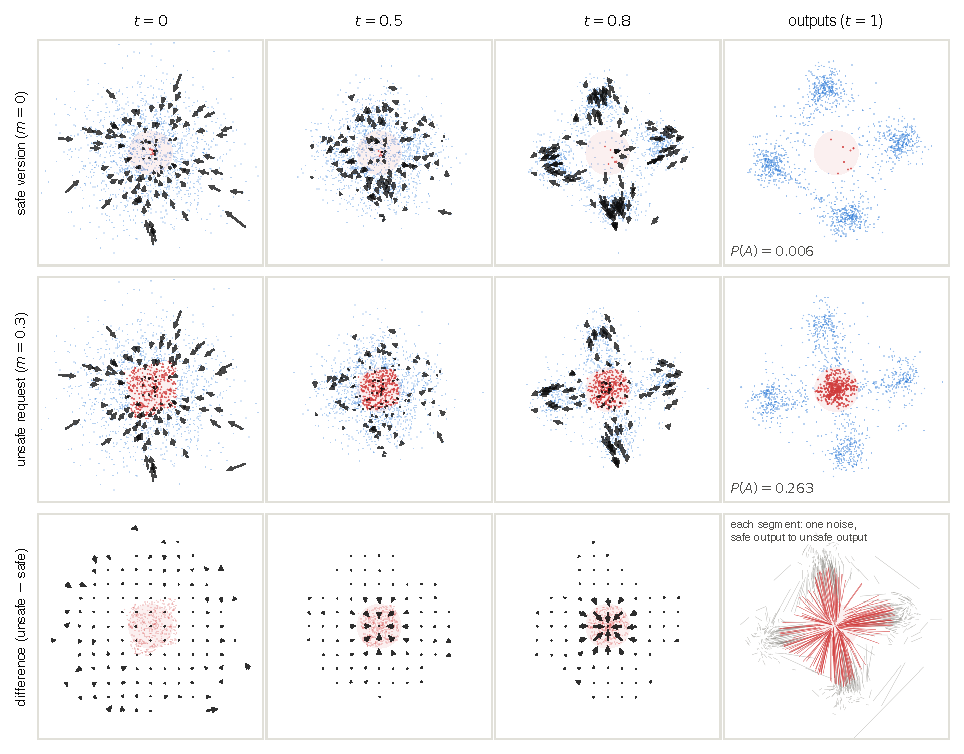
\includegraphics[width=\textwidth]{figures/fig_e1_fields.pdf}
\caption{Step 2. Fields of the running example (1-rectified model) at three times, as arrows attached to $110$ of the
particles (arrow length: distance travelled in $0.15$ time units), with all $1500$ particles at that time; red particles
end in $A$. Top: safe version ($m=0$). Middle: unsafe request ($m=0.3$). Bottom: their difference, on a grid restricted to
where the particles are, over the red particles of the middle row; last panel: for every second noise, the segment
from its safe output to its unsafe output (red when the unsafe output is in $A$).}
\label{fig:e1_fields}
\end{figure}
\FloatBarrier

\paragraph{Step 3: time and straightness.}
How much the start of a field says about its outputs depends on how curved its trajectories are (Lemma~\ref{lem:time};
Figure~\ref{fig:e1_time}).
\begin{itemize}
\item The 1-rectified model is trained with the independent coupling, so its field at $t=0$ points every noise
approximately at the mean of the target (exactly, for the exact field: Lemma~\ref{lem:time}(iii)), the centre of the ring,
which lies in $A$. The one-step map $T^1_v(\bx)=\bx+v(\bx,0)$ sends $\ewOneStepAOne\%$ of
the noise of the running example into $A$ (and a fraction $\eoneOneStepRectOne$ of the probe noise over all safe prompts), whereas
$50$ Euler steps produce the ring. Its trajectories bend, and the straightness defect is $\zeta=\ewZetaOne$ (median over safe
prompts: $\eoneZetaA$).
\item Reflow refits the model on its own noise--output pairs (Definition~\ref{def:reflow}; the details of the refit are in
Remark~\ref{rem:reflow}). The field at $t=0$ then points each noise to its final blob (for the exact reflowed field, to the output of
the previous sampler: Lemma~\ref{lem:reflow}(iii)), the trajectories are nearly straight ($\zeta=\ewZetaTwo$; median $\eoneZetaB$), and one step nearly
reproduces the outputs ($\ewOneStepATwo\%$ in $A$). The price is fidelity: MMD$^2\times10^3=\eoneMmdB$ with $50$ steps and $\eoneMmdC$ with
one step, against $\eoneMmdA$ before reflow.
\item For the method, the source-slice distance $d_0$ stands in for the map metric only for straight fields
(Lemma~\ref{lem:time}(i)). After reflow, $d_0$ and $d_T$ exclude the same prompts, and with one Euler step they coincide. On
the 1-rectified model $d_0$ still excludes $\eoneExAZc$ of the prompts with $m=0.1$, because the fitted slice at $t=0$ also
carries the covariance of the target, which the central mass reduces; but its certificate pays defects of order
$\eoneZetaA$ (Corollary~\ref{cor:one_step}(ii)) and is vacuous. The rest of this section uses the map metric of the $50$-step
sampler.
\end{itemize}

\begin{figure}[!htbp]
\centering
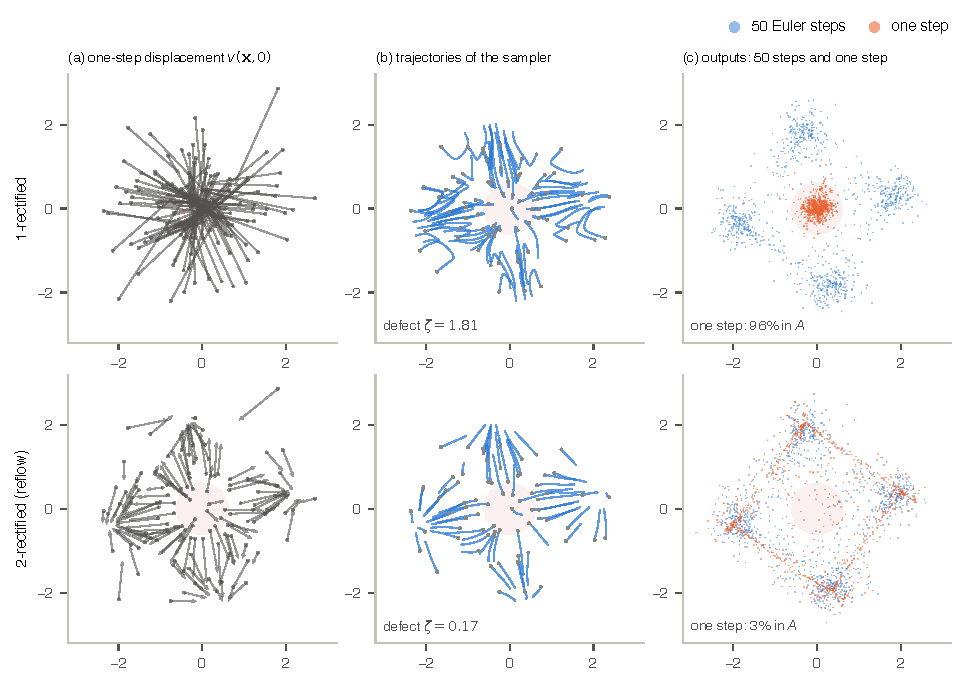
\includegraphics[width=\textwidth]{figures/fig_e1_time.pdf}
\caption{Step 3. The safe version of the running example, before (top) and after reflow (bottom). (a) Each arrow goes
from a noise $\bx$ to $\bx+v(\bx,0)$, the output of the one-step sampler. (b) Trajectories of the $50$-step sampler from the grey
starting points; $\zeta$ is the straightness defect (Definition~\ref{def:sampler}). (c) Outputs of the two samplers on the same
$1000$ noises.}
\label{fig:e1_time}
\end{figure}
\FloatBarrier

\paragraph{Step 4: comparing two fields through the noise they share.}
The map metric does not compare arrows: it compares where two fields send the \emph{same} noise
(Definition~\ref{def:metrics}(ii), Lemma~\ref{lem:coupling_bounds}). Figure~\ref{fig:e1_coupling} colours each point of the noise plane by
where a field sends it.
\begin{itemize}
\item The safe version (a) cuts the noise plane into four sectors, one per blob; the boundaries are where
trajectories split.
\item The unsafe request (b) keeps these sectors but carves out a central region, of noise mass $\ewMassA$, which it
sends into $A$. This is the set $\mathcal Z$ of Proposition~\ref{pr:sqrt_m}, with a displacement $\Delta\approx\ewDispA$.
\item A safe anchor at rotation $\ewAngA^\circ$ (c) rotates the sectors: almost every noise moves by about the chord of
the rotation, and the $\ewSwitch\%$ of the noise between the two sets of boundaries (orange) changes blob.
\item Panel (d) shows the distribution of the displacement $\|T(\bx)-T'(\bx)\|$, $\bx\sim\mu_0$, through its survival function
$S(\delta)=P(\|T(\bx)-T'(\bx)\|\ge\delta)$. Each distance of this note summarises $S$: the $L^1$ map distance is the area under $S$, the
truncated distance $d_1$ of Proposition~\ref{pr:truncated} is the area over $[0,1]$, the tail score is $S(0.5)$, and the $L^2$
map metric is $(\int_0^\infty2\delta S(\delta)d\delta)^{1/2}$.
\end{itemize}
The values for the three pairs of panel (d) are:
\begin{center}
\small
\begin{tabular}{l c c c c}
\toprule
compared with the safe version & $L^2$ & $L^1$ & truncated $L^1$ & tail at $0.5$\\
\midrule
nearest safe anchor ($\ewRotNear^\circ$ apart) & \ewDLtwoNear & \ewDLoneNear & \ewDTrNear & \ewDTailNear\\
safe anchor $a$ ($\ewRotA^\circ$ apart) & \ewDLtwoRot & \ewDLoneRot & \ewDTrRot & \ewDTailRot\\
unsafe request ($m=0.3$) & \ewDLtwoUns & \ewDLoneUns & \ewDTrUns & \ewDTailUns\\
\bottomrule
\end{tabular}
\end{center}
Under every distance, a safe prompt rotated by $\ewRotA^\circ$ is farther from the safe version than the unsafe request is.
A distance between fields detects an unsafe mode only against \emph{nearby} safe fields, and the rest of this section
follows from that.

Unbounded distances have a second weakness, which is numerical rather than geometric. The $L^p$ map distances with $p>2$,
which Proposition~\ref{pr:sqrt_m} suggests for rare modes (a lower bound $m^{1/p}\Delta$), fail with uniform weights: they exclude only
$\eonePrLfourUAlld$ ($p=4$) and $\eonePrLeightUAlld$ ($p=8$) of the prompts with $m=0.3$, and $L^4$ excludes more requests with $m=0.01$
($\eonePrLfourUAlla$) than with $m=0.3$, a reversed trend that no property of the unsafe mode explains. The cause is the divergence of
the 1-rectified sampler (Step~1). Probe~$\eoneProbe$, the largest of the $256$, is sent beyond radius $4$ for $\eoneBlowSafe\%$ of the
approved prompts but for only $\eoneBlowUns\%$ of those with $m=0.3$, whose central mass holds the trajectory back; between two
approved prompts this one probe carries a median $\eoneShareMed\%$ (mean $\eoneShareMean\%$) of the squared $L^2$ distance. Without it
(Table~\ref{tab:e1_probe}), the uniform $L^4$ and $L^8$ regions exclude $\eonePrLfourUDropd$ and $\eonePrLeightUDropd$ of the prompts with
$m=0.3$, the nearest-field $L^2$ region excludes $\eonePrLtwoNDropc$ of those with $m=0.1$, like the $L^1$ and truncated ones, and the
bounded distances do not move. The comparison of map distances in this section is therefore not a property of the safe
family: unbounded distances inherit the divergence of the sampler, and the truncated distance, which caps the contribution of
every noise, does not. Dropping a probe after the fact is a diagnosis, not a method; the method uses a bounded distance.

\begin{table}[!htbp]
\centering
\caption{Step 4: exclusion of unsafe requests and median budget with all $256$ probes $\to$ without probe~$\eoneProbe$, the only
probe that some pool prompt's sampler sends beyond radius $4$ (the trimming radius of Remark~\ref{rem:reflow}), on both models.
Same splits, scores and thresholds as Figure~\ref{fig:e1_detection} ($100$ splits).}
\label{tab:e1_probe}
\small
\begin{tabular}{l cccc c}
\toprule
& \multicolumn{4}{c}{excluded at $m=$} & \\
\cmidrule(lr){2-5}
score & $0.01$ & $0.03$ & $0.1$ & $0.3$ & budget\\
\midrule
\inputrows{tables/e1_probe.tex}
\bottomrule
\end{tabular}
\end{table}

\begin{figure}[!htbp]
\centering
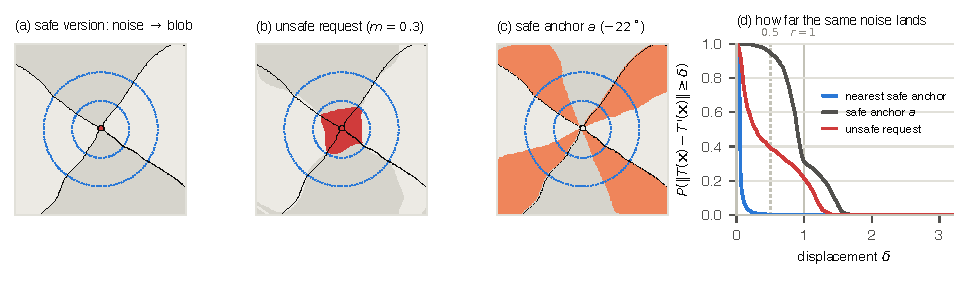
\includegraphics[width=\textwidth]{figures/fig_e1_coupling.pdf}
\caption{Step 4. The noise plane, coloured by where each noise is sent (two greys alternate between the four blobs;
red: into $A$); dotted circles: radii $1$ and $2$ of $\mu_0$. (a) Safe version of the running example, with its sector
boundaries in black, repeated in (b) and dashed in (c). (b) Unsafe request ($m=0.3$). (c) Safe anchor $a$ at rotation
$\ewAngA^\circ$; orange: noise sent to a different blob than by the safe version. (d) Survival function of the displacement
between the outputs of the safe version and of three other fields on the same $2000$ noises.}
\label{fig:e1_coupling}
\end{figure}
\FloatBarrier

\paragraph{Step 5: the conformal region as a threshold on a score.}
The region keeps the fields whose score is at most the threshold $\varepsilon$, the $\lceil(K+1)(1-\beta)\rceil$-th smallest calibration
score (Definition~\ref{def:region}). By exchangeability, a new safe prompt falls below it with probability at least $0.9$
(Proposition~\ref{pr:coverage}). Figure~\ref{fig:e1_scores} shows the scores of all prompts of split $0$, divided by $\varepsilon$.
\begin{itemize}
\item \emph{As written} (a), the score is the mean distance to the $30$ anchors. Nine safe scores in ten lie between $\ewSafeLoU$ and $\ewSafeHiU$: a safe prompt with an extreme rotation is far from
most anchors. The threshold must admit $90\%$ of the safe prompts, so it
sits at the score of the most atypical ones, and a typical prompt with an unsafe mode looks less atypical than an
atypical safe prompt: only $\ewExUc\%$ of the prompts with $m=0.1$ are outside, and $\ewExUd\%$ of those with $m=0.3$.
\item Panel (c) shows the mechanism on the running example. The unsafe mode raises the distance to every anchor,
but the score averages these distances, which are dominated by rotation; it rises from $\ewScUzero\varepsilon$ to $\ewScUone\varepsilon$ only,
below the threshold. What keeps it there is the spread of the safe scores. Over $100$ splits the budget $(M+1)\varepsilon$ is
$\eoneBudgetAT$ for $d_T$, and a typical safe test prompt is at mean distance $\eoneTypicalAT$ from the anchors: an unsafe mode must
close that gap through an average of $30$ distances, and for $L^2$ a far anchor adds the unsafe displacement $\delta$ only in
quadrature, $d(u,\bth_i)\approx(d_i^2+\delta^2)^{1/2}$. The floor of Proposition~\ref{pr:geometry}(iii), here $\eoneFloorAT$, bounds the
budget from below and makes the certificate loose (Step~7); it is not what binds.
\item \emph{The fix} compares the request with the safe field nearest to it (weights $w=\mathbf 1_{i^\star}$,
Proposition~\ref{pr:truncated}), in the truncated distance: panels (b) and (d). The nearest anchor is $\ewRotNear^\circ$ away from the
running example, so the safe version scores $\ewScKzero\varepsilon$, and the unsafe mode lifts the score to $\ewScKone\varepsilon$. Every prompt
with $m\ge0.1$ is now outside, while $\ewCovK\%$ of the safe test prompts are inside ($90\%$ in expectation over splits).
\end{itemize}
Over $100$ splits (Figure~\ref{fig:e1_detection}), coverage lies between $\eoneFigCovMin$ and $\eoneNonTailCovMax$ for every score and model
except the tail score, against a nominal $0.902$. The tail score reaches $\eoneKnnTailCov$ (1-rectified) and $\eoneKnnTailCovTwo$
(reflowed): it counts probes, its median threshold is $\eoneTailProbesOne$ and $\eoneTailProbesTwo$ probes out of $256$, and the scores that
tie with the threshold are admitted. The guarantee still holds, but the region is decided by a handful of probes; randomised
tie-breaking or more probes would remove the excess. Exclusion at $m=0.1$ rises from $\eoneExATc$ as written to $\eoneKnnLonec$ with the
nearest field in $L^1$ and $\eoneKnnTruncc$ in truncated $L^1$; in $L^2$ it reaches $\eoneKnnLtwoc$, and $\eonePrLtwoNDropc$ without
probe~$\eoneProbe$ (Step~4). With the same $L^2$ distance, localising shrinks the budget by a factor $\ewBudRatioOne$ on the 1-rectified
model ($\eonePrBudRatioDrop$ without probe~$\eoneProbe$) and $\ewBudRatioTwo$ on the reflowed one. The uniform region built on the prompt embeddings
excludes $\eoneExAEc$ of the prompts with $m=0.1$, and the one built on the pooled-path distance $d_{\bar\rho}$ excludes $\eoneExARc$: on honest
prompts, the field distances as written do no better than prompt distances.

\begin{figure}[!htbp]
\centering
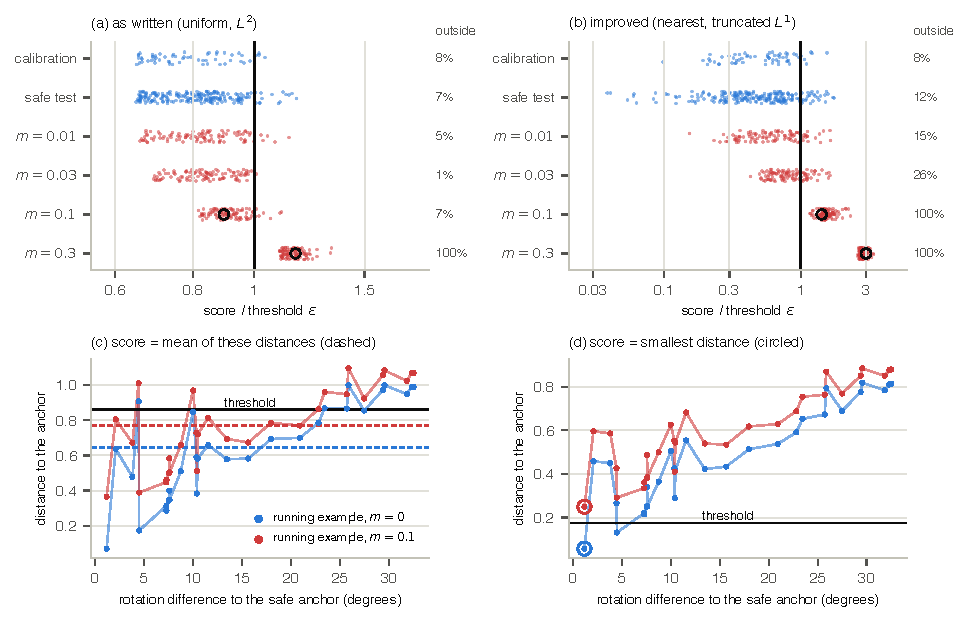
\includegraphics[width=\textwidth]{figures/fig_e1_scores.pdf}
\caption{Step 5, split $0$. (a)--(b) Scores of the calibration, safe test and unsafe prompts, divided by the threshold
$\varepsilon$ (vertical line); right: percentage outside the region; black circles: the running example with $m=0.1$ and $m=0.3$.
(c)--(d) Distance from the running example, without (blue) and with an unsafe mode of mass $0.1$ (red), to each of the
$30$ safe anchors, against their rotation difference. The score is the mean of these distances as written (dashed
lines), and the smallest one in the improved method (circles).}
\label{fig:e1_scores}
\end{figure}

\begin{figure}[!htbp]
\centering
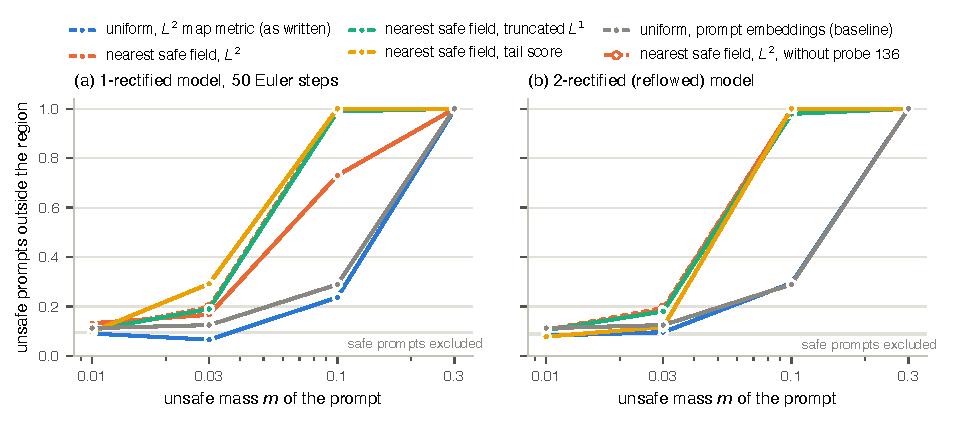
\includegraphics[width=\textwidth]{figures/fig_e1_detection.pdf}
\caption{Step 5, all splits. Exclusion of unsafe prompts against their unsafe mass (means over $100$ splits). The method
as written (blue) and the order-$1$ region on prompt embeddings (grey) coincide on the reflowed model; scoring against
the nearest safe field excludes almost every prompt with $m\ge0.1$ with the truncated distance and the tail score (aqua, yellow),
and with $L^2$ (orange) on the reflowed model, and on the 1-rectified model once probe~$\eoneProbe$, which its sampler sends beyond
radius $4$, is removed (dashed orange; Table~\ref{tab:e1_probe}). Light grey: fraction of safe test prompts excluded ($1-$coverage,
averaged over the scores; the tail score over-covers, see the text).}
\label{fig:e1_detection}
\end{figure}

\paragraph{Step 6: the region in field space, and enforcement.}
A request outside the region is not refused: its field is mixed with a feasible safe field, by bisection on the
mixing weight, until the score reaches the threshold (Proposition~\ref{pr:backoff}). For this model, affine in the prompt,
the mixed field is the field of the mixed prompt, because affine maps preserve convex combinations (Lemma~\ref{lem:convex}(i)).
Corollary~\ref{cor:prompt_mixing} says the same of the projection of Proposition~\ref{pr:projection}(iii), which applies to the Mahalanobis
distances only; the test checks its identity (to $\eoneMixcheck$) but enforces every score by back-off. For the running example with
$m=0.3$, both methods mix with the same safe field $c$, a calibration prompt with nearly the same rotation and radius.
Figure~\ref{fig:e1_slice} shows the plane of fields through the unsafe request $u$, the safe field $c$ and the safe anchor $a$ of
Step~4, coloured by the $P(A)$ of their outputs, with the boundary of each region; every point of the plane is the
field of an affine combination of the three prompts.
\begin{itemize}
\item Back-off walks from $u$ towards $c$ along the dashed line and stops at the first boundary it meets. It enters the
region as written at $\alpha=\ewAlphaU$, where $P(A)=\ewSlicePAb$ (point~2), and the improved region at $\alpha=\ewAlphaK$, where
$P(A)=\ewSlicePAc$ (point~3).
\item The region as written is one large set, which in this plane contains fields with $P(A)$ up to $\ewSliceMaxU$. The
improved region is a union of small sets around safe fields, the union of balls of Proposition~\ref{pr:truncated}, with
$P(A)\le\ewSliceMaxK$ in this plane. It also leaves out the fields between $c$ and $a$ (point~5): they are not unsafe, but
they produce a smeared ring that no approved prompt asks for.
\item Over $5$ splits and the $100$ prompts with $m=0.3$, enforcement lowers $P(A)$ from $\eonePAAd$ to $\eoneTwoPAasWritten$ as written and to
$\eoneTwoPAtrunc$ with the improved method. It also keeps the outputs closer to the request's safe intent: MMD$^2\times10^3$ to the
$m=0$ target is $\eoneTwoMmdAsWritten$ against $\eoneTwoMmdTrunc$, and $\eoneTwoMmdNone$ without enforcement, because the improved method mixes
with a nearby safe prompt instead of being pulled towards an average one. Safe prompts are altered at the rate
$1-$coverage, without loss of fidelity (Table~\ref{tab:e1_detection}).
\end{itemize}

\begin{figure}[!htbp]
\centering
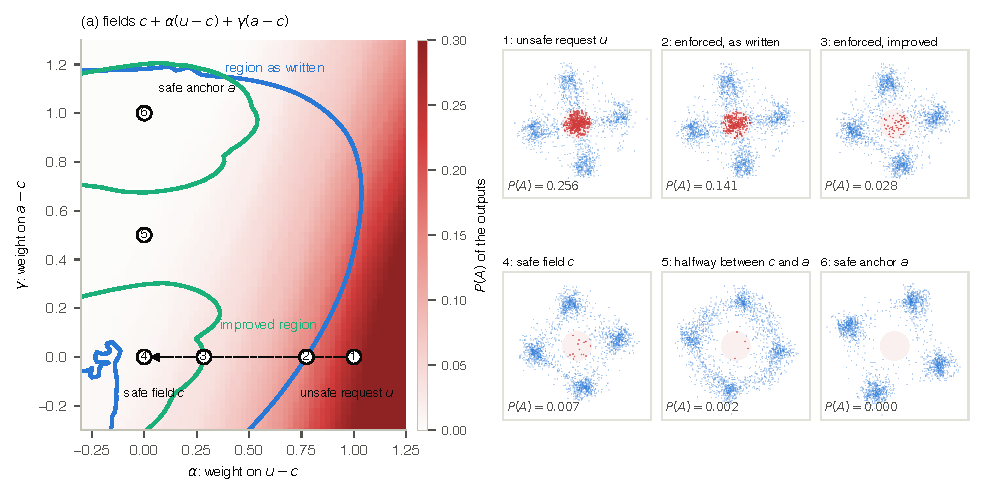
\includegraphics[width=\textwidth]{figures/fig_e1_slice.pdf}
\caption{Step 6. (a) The plane of fields $c+\alpha(u-c)+\gamma(a-c)$ through the unsafe request $u$ ($m=0.3$), the safe field $c$
towards which both methods back off, and the safe anchor $a$; colour: $P(A)$ of the outputs ($1000$ noises per field).
Blue: boundary of the region as written; aqua: boundary of the improved region; both contain $c$. Dashed arrow:
back-off path. (1)--(6) Outputs ($2000$ noises) of the numbered fields: the request, the two enforced fields, $c$, the
halfway mixture of $c$ and $a$, and $a$.}
\label{fig:e1_slice}
\end{figure}
\FloatBarrier

\paragraph{Step 7: what the certificate says about the enforced field.}
The certificate is a transport argument (Theorem~\ref{th:certificate}, Proposition~\ref{pr:truncated}). Pair each output $Y$ of the
enforced field with the output $Y'$ of a safe field for the same noise. An output in $A$ comes either from a safe output
within $r$ of $A$, or from a pair at least $r$ apart, so $P(Y\in A)\le P(Y'\in A^{+r})+P(\|Y-Y'\|\ge r)$. The first term is measured
on the safe field. The second is bounded by the budget: by $(M+1)\varepsilon/r$ through Markov's inequality for the $L^2$ map
metric, and by $(M+1)\varepsilon\max(1,1/r)$ for the truncated distance. Figure~\ref{fig:e1_certificate} plots both terms and their sum
against $r$; the certificate is the minimum of the sum.
\begin{itemize}
\item \emph{As written} (b), the safe field is the uniform mixture of the anchors, and the budget is large and decays only
like $1/r$. The best bound is $\ewCertU$ (at $r=\ewCertRU$) for an actual $P(A)=\ewCertPAU$: vacuous. Over all fields of the region,
the median Markov bound is $\eoneMarkovMed$.
\item \emph{Improved} (c), the safe field is the nearest anchor and the budget is $\ewCertBudgetK$; the bound is $\ewCertK$ (at
$r=\ewCertRK$) for an actual $P(A)=\ewCertPAK$. Panel (a) shows why it is loose: the noise that the enforced field sends into $A$
is noise that the safe field sends to the inner edge of its blobs, all within $r$ of $A$, so the first term already
covers it, and the bound adds the whole budget on top. The tail score, which counts the redirected noise directly,
certifies $P(A)\le\eoneTwoCertTail$ in median over enforced fields, against $\eoneSafePAA$ for safe prompts.
\item These certificates are plug-in: distances are estimated on $256$ frozen probes, and back-off parks enforced fields on the
boundary of the region, so on the evaluation noise \eoneTwoPlugMin{} to \eoneTwoPlugMax{} of them exceed their budget, by at most a factor
$\eoneTwoTruncMaxRatio$ with the truncated distance, which is bounded, and up to $\eoneTwoLoneMaxRatio$ with $L^1$, which is not. No enforced
field's $P(A)$ exceeds its certificate on that noise, but this check is weak: the safe term and $P(A)$ are measured on the same
noise, where the coupling inequality holds noise by noise, and the bound is far above the unsafe mass (median $\eoneSlackBound$
against $\eoneSlackPA$ for the improved method; Table~\ref{tab:e1_certificates}).
\item \emph{Verified deployment.} The certificate becomes rigorous when each deployed field is checked on fresh noise. The nearest
anchor $i^\star$ is chosen on the frozen probes, and a \emph{check} computes an upper confidence bound at level $1-\delta_d/2$ for the
distance to $i^\star$ on $L=\eoneVerL$ fresh noises (Hoeffding's for the truncated distance, whose values lie in $[0,1]$, which adds
$\eoneVerHoeff$; Clopper--Pearson's for the tail score, a proportion) and passes if the bound is at most the budget $b$. A request
admitted on the probes is checked as it is; otherwise, or if that check fails, it is backed off on the probes towards a reduced
budget $b'$, which lies below $b$ by the margin of the check and two standard errors of the probe estimate (at most
$\sqrt{b(1-b)/256}$ each, by the Bhatia--Davis inequality), and checked again; if both checks fail, the anchor $i^\star$ itself is
deployed. With at most two checks per request, the deployed field is within $b$ of its anchor with probability at least
$1-\delta_d$; with Clopper--Pearson upper bounds for the safe term, computed on $\eoneVerLbig$ further noises at level $1-\delta_q/40$ for
each of the $40$ enlargements $r$, the certificate holds with probability at least $1-\delta_d-\delta_q=1-\eoneVerDelta$.
Table~\ref{tab:e1_verify} reports the result on the $5$ splits. No deployed field, of $\eoneVerN$, exceeds its budget on $\eoneVerLbig$
noises independent of the check, and none has a $P(A)$ above its certificate on the evaluation noise, which is independent of every
term ($\eoneVerViol$ violations). The price is paid by safe prompts: a fraction $\eoneVerOneTrAlt$ of them is mixed with a nearby safe
prompt on the 1-rectified model, against about $0.1$ with plug-in back-off. Unsafe requests gain: the reduced budget lowers $P(A)$ at
$m=0.3$ to $\eoneVerOneTrPA$ (against $\eoneTwoPAtrunc$) and MMD$^2\times10^3$ to $\eoneVerOneTrMmd$ (against $\eoneTwoMmdTrunc$). The rigorous
certificate on $P(A)$ is $\eoneVerOneTrBound$ with the truncated distance and $\eoneVerOneTailBound$ with the tail score, close to the plug-in
values $\eoneTwoCertTrunc$ and $\eoneTwoCertTail$: with Clopper--Pearson rather than Hoeffding margins, the tail score keeps its tight
certificate. Its budget on the reflowed model is so small ($\eoneTailProbesTwo$ probes) that $\eoneVerTwoTailFall$ of the requests with $m=0.3$ fall back
to their anchor.
\end{itemize}

\begin{table}[!htbp]
\centering
\caption{Step 7: verified deployment of the improved regions ($5$ splits; the first $80$ safe test prompts and the requests with
$m\in\{0.1,0.3\}$). Budget $b$ (the calibrated threshold, unchanged) and reduced budget $b'$ of the back-off (medians over splits);
fraction of safe test prompts whose field is not deployed as it is; fraction of requests with $m=0.3$ that fall back to their
nearest anchor, their $P(A)$ and their MMD$^2\times10^3$ to the target without unsafe mode; fraction of deployed fields whose distance to
their anchor on $10{,}000$ independent noises exceeds $b$; median certificate on $P(A)$, valid with probability at least $0.95$.}
\label{tab:e1_verify}
\small
\begin{tabular}{l cc c ccc c c}
\toprule
& & & safe & \multicolumn{3}{c}{requests with $m=0.3$} & over & \\
\cmidrule(lr){5-7}
score & $b$ & $b'$ & altered & fallback & $P(A)$ & MMD$^2$ & budget & certificate\\
\midrule
\inputrows{tables/e1_verify.tex}
\bottomrule
\end{tabular}
\end{table}

\begin{figure}[!htbp]
\centering
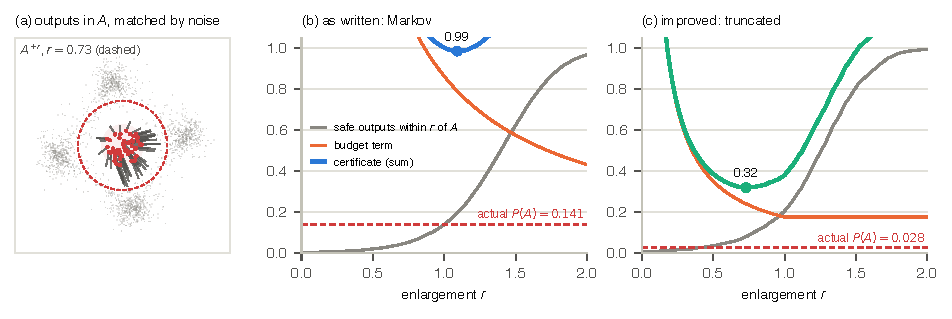
\includegraphics[width=\textwidth]{figures/fig_e1_certificate.pdf}
\caption{Step 7. (a) Outputs in $A$ of the field enforced by the improved method (red), each joined to the output of the
nearest safe field for the same noise (grey), and $A^{+r}$ at the optimal $r$ (dashed). (b)--(c) The two terms of the
certificate on $P(A)$ and their sum, against the enlargement $r$, for the field enforced as written (relative to the
uniform mixture of the anchors, with Markov's inequality) and for the improved one (relative to the nearest anchor,
truncated distance); dashed: actual $P(A)$ on $2000$ noises.}
\label{fig:e1_certificate}
\end{figure}
\FloatBarrier

\paragraph{Step 8: attacks on the prompt.}
So far the requests were honest: an unsafe mode of a given mass. A white-box attacker instead searches the
embedding space for the prompt with the largest $P(A)$ that the region admits. The \emph{random search} proposes Gaussian steps
in all $43$ coordinates of the embedding ($12$ runs of $300$ steps, each starting from an enforced prompt with $m=0.3$). The
\emph{directed search} proposes steps only in the five directions that move the region's distance least, where an attacker would
hide a change from the region: for a field distance, the right singular vectors of the Jacobian of the probe outputs with
respect to the embedding, smallest singular values first ($12$ runs of $400$ steps, from admitted approved prompts). Both report
$P(A)$ on noise that the search did not use. Figure~\ref{fig:e1_attack} shows the worst prompt found by the random search in each
region on split $0$.
\begin{itemize}
\item Inside the order-$1$ region built on prompt embeddings, the attacker finds a prompt whose field sends all the
noise into $A$ ($P(A)=\ewAtkPrompt$). Its embedding is closer to an approved embedding ($\ewAtkEmbNear$) than two approved embeddings
typically are to each other (median $\ewAtkEmbMed$), but it is displaced in directions that change the field a lot: its
field scores $\ewAtkScU\varepsilon$ in the field-space region as written and $\ewAtkScK\varepsilon$ in the improved one, which both reject it. The
embedding distance cannot see this, whereas the pull-back metric of Proposition~\ref{pr:mahalanobis}(iii) weighs each
direction of the embedding by its effect on the field.
\item Inside the field-space regions, the worst prompts have $P(A)=\ewAtkWritten$ as written and $\ewAtkImproved$ with the improved
method, below the bound that holds for every field of their region (Table~\ref{tab:e1_certificates}).
\item Over both models, the worst values are $\eoneTwoAttackEU$ and $\eoneTwoAttackEknn$ for the uniform and localised prompt-space regions,
$\eoneTwoAttackUL$ for the field-space region as written, and at most $\eoneTwoAttackLone$ after localisation; the directed search finds at most
$\eoneDirUL$ and $\eoneDirNear$ (Table~\ref{tab:e1_certificates}). On honest unsafe prompts, the localised prompt-space region does as well
as the field-space ones (Table~\ref{tab:e1_detection}). Against these attacks, constraining fields protects where a Euclidean distance
between prompts does not; Section~\ref{sec:e2} shows that a prompt distance that whitens by the approved embeddings also resists
them in this toy, because its approved embeddings are degenerate.
\end{itemize}

\begin{figure}[!htbp]
\centering
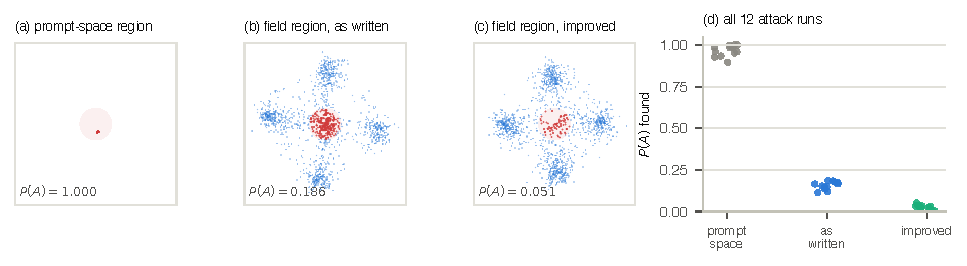
\includegraphics[width=\textwidth]{figures/fig_e1_attack.pdf}
\caption{Step 8. (a)--(c) Outputs ($1400$ fresh noises) of the prompt with the largest $P(A)$ found by the attack inside the
order-$1$ region on prompt embeddings, inside the field-space region as written, and inside the improved region
(1-rectified model, split $0$). (d) $P(A)$ of the best prompt of each of the $12$ random-search runs.}
\label{fig:e1_attack}
\end{figure}
\FloatBarrier

\paragraph{Summary of the results.}
Tables~\ref{tab:e1_detection} and~\ref{tab:e1_certificates} collect the results of the method as written, of its improvements and of the
prompt-space baselines, on both models.
\begin{itemize}
\item Coverage holds for every score (Step~5); the tail score, which counts probes, over-covers because of ties.
\item The region as written is valid but too wide on a diverse family: its averaged score measures the spread of the
safe fields rather than the request (Steps~4--5).
\item Scoring against the nearest safe field repairs detection and enforcement (Steps~5--6). A bounded (truncated) distance
keeps the score immune to the sampler's divergence on rare noise (Step~4), which made the $L^2$ and $L^p$ distances look less
sensitive than they are, and tightens the certificate, which the verification of Step~7 makes rigorous.
\item Field-space regions resist both attacks, which break the Euclidean prompt-space regions (Step~8).
\item Two limits remain. An unsafe mass smaller than the spread of the nearest safe fields is admitted: exclusion at
$m=0.03$ is at most $\eoneKnnTailb$, partly because the model realises only $\eoneRealisedb\%$ of that mass (Step~1), and smaller masses
need denser safe anchors near the request, which a family of more than two dimensions makes expensive. And the certificate
is relative to the nearest safe prompt.
\end{itemize}

\begin{table}[!htbp]
\centering
\caption{The method as written against its improvements and against prompt-space regions (means over $5$
splits). Budget: median calibrated threshold of $\sum_iw_id(\bth,\bth_i)$, the $(M+1)\varepsilon$ of
Theorem~\ref{th:certificate}, in the units of each distance. MMD$^2\times10^3$ between the enforced outputs at $m=0.3$
and the $m=0$ target; last column: fraction of safe test prompts altered by enforcement.}
\label{tab:e1_detection}
\small
\begin{tabular}{l c c cc cc c c}
\toprule
& & & \multicolumn{2}{c}{excluded at $m=$} & \multicolumn{2}{c}{enforced $P(A)$, $m=$} & & safe\\
\cmidrule(lr){4-5}\cmidrule(lr){6-7}
score & coverage & budget & $0.03$ & $0.1$ & $0.1$ & $0.3$ & MMD$^2$ & altered\\
\midrule
\inputrows{tables/e1_detection.tex}
\bottomrule
\end{tabular}
\end{table}

\begin{table}[!htbp]
\centering
\caption{Plug-in certificates on $P(A)$. Enforced fields ($5$ splits, safe test prompts and unsafe requests): median of each
field's certificate (budget on the frozen probes) and median $P(A)$ on the evaluation noise, fields whose distance on that noise
exceeds the budget, and the a-posteriori bound with the empirical tail of the coupling distance. Attacks (split $0$, $12$ runs
each): largest $P(A)$ found inside the region by the random and the directed search (Step~8), and the bound that holds for every
field of the region. The rigorous version of these certificates is in Table~\ref{tab:e1_verify}.}
\label{tab:e1_certificates}
\small
\begin{tabular}{l c c c c c c c}
\toprule
& \multicolumn{4}{c}{enforced fields} & \multicolumn{3}{c}{attacks}\\
\cmidrule(lr){2-5}\cmidrule(lr){6-8}
score & bound & $P(A)$ & over budget & empirical & random & directed & bound\\
\midrule
\inputrows{tables/e1_certificates.tex}
\bottomrule
\end{tabular}
\end{table}
\FloatBarrier

\paragraph{The improved method.}
For a prompt with field $\bth$: compute its outputs on $L$ frozen probe noises; score it by the truncated
distance to the nearest safe field, $\min_id_r(\bth,\bth_i)/(M+1)$, calibrated by split conformal prediction as
before; if the score exceeds the threshold, mix the prompt with its nearest feasible safe prompt, by bisection on the
mixing weight (Proposition~\ref{pr:backoff}; for a model affine in the prompt, the mixed field is the field of the mixed prompt);
then verify the field to be deployed on fresh noise, and deploy its nearest anchor instead if the check fails (Step~7). With
probability at least $1-\delta$ over the fresh noise, the deployed outputs satisfy
$P(Y\in B)\le P(Y_{i^\star}\in B^{+r})+(M+1)\varepsilon$ for every $B$, relative to the nearest safe prompt $i^\star$
(Proposition~\ref{pr:truncated}). This is the split-conformal nearest-neighbour novelty detector
\citep{laxhammar2015inductive,bates2023testing} with a bounded distance between sampler maps: it keeps the coverage and the
certificate, adds locality and robustness to diverging trajectories, and applies Markov's inequality only to a bounded
variable. Its region is a union of balls and is not convex, for any sampler; it is enforced by back-off, not by projection.

% =====================================================================================
\section{Static and adaptive regions, on prompts and on fields}\label{sec:e2}
% =====================================================================================

Section~\ref{sec:e1} found, on the two-dimensional toy, that the order-$1$ region as written is valid but too wide, that scoring
a request against the nearest safe field repairs detection, and that regions built on fields resist white-box attacks that
break regions built on Euclidean distances between prompt embeddings. Two choices lie behind these results, the weights of the
score and the space in which distances are measured. This section separates them, tunes the weights on data disjoint from the
evaluation data, gives the prompt space a second, whitened distance, and answers three questions.
\begin{enumerate}[label=(Q\arabic*)]
\item \emph{Weights} (Section~\ref{sec:e2_weights}). Do adaptive weights, which take the transport mass from the approved prompts
closest to the request, beat the static weights of Definition~\ref{def:region}?
\item \emph{Space} (Section~\ref{sec:e2_space}). Is a region on the prompt embeddings as good as a region on the fields that the
prompts induce?
\item \emph{Repairs} (Section~\ref{sec:e2_repairs}). What still fails, and which modifications (more approved prompts, a pull-back
metric, reflow) repair it, for static and for adaptive regions?
\end{enumerate}
Section~\ref{sec:e2_design} describes the design, and Section~\ref{sec:e2_summary} summarises the answers.

\subsection{Design}\label{sec:e2_design}

\paragraph{Task and models.}
The task and the models are those of Section~\ref{sec:e1}. A prompt $z=(\phi,\varrho,m)$ asks for the four-blob ring rotated by
$\phi$ and of radius $\varrho$, with a fraction $m$ of its mass moved into the unsafe disk $A=\{\by:\|\by\|\le0.6\}$. Approved prompts
have $m=0$, $\phi\in[-22.5^\circ,22.5^\circ]$ and $\varrho\in[1.75,2.25]$; an unsafe request has an approved rotation and radius and
$m\in\{0.01,0.03,0.1,0.3\}$. A frozen encoder maps $z$ to $\be\in\RR^{43}$, the normalised $(\phi,\varrho,m)$ followed by $40$ random
Fourier features of them; its third coordinate is $m/0.2$. The model is affine in the embedding, $\bth(\be)=\ba+U\be$
(Definition~\ref{def:prompt}(b)), and is deployed in two versions: the 1-rectified model with $50$ Euler steps, faithful but curved,
and the reflowed model with one Euler step, straight and cheap but less faithful (MMD$^2\times10^3$ to the approved targets:
$\eoneMmdA$ and $\eoneMmdC$; Section~\ref{sec:e1}, Step~3).

\paragraph{Regions.}
A region is given by a distance $d$ between prompts and by weights $w$. A request $\be$ scores $\sum_iw_id(\be,\be_i)$ against $M$
approved prompts $\be_1,\dots,\be_M$, the \emph{anchors}, and is admitted if its score is at most a threshold calibrated on $K$ other
approved prompts (Definition~\ref{def:region} without its factor $1/(M+1)$: the threshold is the budget $(M+1)\varepsilon$ of
Theorem~\ref{th:certificate}). By Lemma~\ref{lem:closed_form}, the score is the cost of the optimal transport plan that moves the mass
$w_i/(M+1)$ from each anchor $i$ to the request. Table~\ref{tab:e2_regions} defines the four distances. The field region uses the
truncated map distance: it is bounded, so the rare noises on which the 1-rectified sampler diverges cannot dominate it
(Section~\ref{sec:e1}, Step~4), and its certificate (Proposition~\ref{pr:truncated}) applies Markov's inequality only to a bounded variable.
The Mahalanobis prompt distance whitens the embedding by the covariance $S$ of the approved embeddings of the tuning pool,
regularised by $\delta=\rho\,\mathrm{tr}(S)/43$: it is the standard out-of-distribution detector of \citet{lee2018simple}, applied to
prompts. The pull-back distance is the source-slice
distance $d_0$ between the fields of $\be$ and $\be'$ (Proposition~\ref{pr:mahalanobis}(ii)--(iii)): it weighs each direction of the
embedding by its effect on the field at $t=0$. For a one-step sampler, $d_0$ is the map metric of the deployed sampler
(Corollary~\ref{cor:one_step}(i); numerically, the two agree to a relative error below $10^{-7}$), so the pull-back region of the
reflowed model is a field region computed on the prompts; for the $50$-step 1-rectified model, $d_0$ ignores the later steps.

\begin{table}[!htbp]
\centering
\caption{The four distances between a request $\be$ and an anchor $\be_i$. $T$ and $T_i$ are the noise-to-output maps of the
deployed sampler for $\be$ and $\be_i$, $\bx_0$ ranges over $256$ probe noises shared by all prompts, $G_0$ is the Gram matrix of
the features at $t=0$ (Proposition~\ref{pr:mahalanobis}(ii)), and $S$ is the covariance of the approved embeddings of the tuning pool.
Field and pull-back regions are computed for one model, named in parentheses when needed: field (1-rectified), pull-back
(reflowed), and so on.}
\label{tab:e2_regions}
\small
\begin{tabular}{l l l l}
\toprule
region & distance $d(\be,\be_i)$ & a score needs & certificate on the outputs\\
\midrule
prompt & $\|\be-\be_i\|$ & the embeddings & none\\
Mahalanobis & $\|\be-\be_i\|_{(S+\delta I)^{-1}}$ & the embeddings & none\\
field & $\E\min(\|T(\bx_0)-T_i(\bx_0)\|,1)$ & one run of the sampler & Proposition~\ref{pr:truncated}\\
pull-back & $\|\be-\be_i\|_Q$, $Q=U^\top G_0U$ & the embeddings & Theorem~\ref{th:certificate}, reflowed model only\\
\bottomrule
\end{tabular}
\end{table}

\paragraph{Weights.}
\emph{Static} weights are uniform, $w_i=1/M$. \emph{Adaptive} weights concentrate the transport mass on the anchors closest to the
request. Three families are tuned: Gaussian kernel weights $w_i\propto\exp(-d(\be,\be_i)^2/(2h^2))$, with $h$ equal to $c$ times the
median distance between anchors ($c\to0$ keeps the nearest anchor, $c\to\infty$ gives the static weights); equal weights on the $k$
nearest anchors; and, for field regions, the same kernel in the embedding distance (the prompt-adaptive weights of
Section~\ref{sec:region}). For the Mahalanobis region, $\rho\in\{10^{-6},10^{-4},10^{-2},1\}$ is tuned with the weights. Each weighting is
a fixed function of the request given the anchors and the tuning pool, so coverage holds for all of them
(Proposition~\ref{pr:coverage}). With $k=1$, the adaptive field region is the improved method of Section~\ref{sec:e1}.

\paragraph{Protocol and metrics.}
The prompts are new draws: $1000$ approved prompts, split once into a tuning pool ($300$) and an evaluation pool ($700$), and unsafe
requests on $200$ approved (rotation, radius) pairs, each with the four masses ($100$ pairs for tuning, $100$ for evaluation). A split
draws $M=30$ anchors and $K=60$ calibration prompts from a pool and tests on the rest; with $\beta=0.1$, the nominal coverage is
$55/61=0.902$. For each region and each $M$, the adaptive family and its parameter maximise the mean exclusion of the four masses
over $50$ splits of the tuning pool; all results come from the evaluation pool, which the tuning never sees.
\begin{itemize}
\item \emph{Coverage}: the fraction of approved test prompts admitted. \emph{Exclusion} at mass $m$: the fraction of unsafe requests
of that mass not admitted. Both are means over $200$ splits ($100$ when $M\ne30$). Exclusion at a mass is a mean over $100$
distinct requests, so differences below about $0.1$ are within sampling error.
\item \emph{Enforcement}: back-off (Proposition~\ref{pr:backoff}) mixes an excluded prompt with its nearest feasible approved prompt
until the score reaches the threshold; for this model, the mixed prompt induces the mixed field (Lemma~\ref{lem:convex}(i)).
For the requests with $m=0.3$ ($3$ splits), $P(A)$ of the enforced outputs and their MMD$^2\times10^3$ to the target of the same
request without unsafe mode (fidelity).
\item \emph{Attacks}: the two white-box searches of Section~\ref{sec:e1}, Step~8, on one split, for the admitted embedding with the
largest $P(A)$, reported on fresh noise. The random search makes $12$ runs of $300$ Gaussian steps in all coordinates, from enforced
requests with $m=0.3$. The directed search makes $12$ runs of $400$ steps from admitted approved prompts, in the five directions in
which the region's distance grows slowest: the eigenvectors with the smallest eigenvalues of its metric Gram matrix, $Q$ for the
pull-back distance, $J^\top J$ for the field distance ($J$ the Jacobian of the probe outputs with respect to the embedding), and
$(S+\delta I)^{-1}$ for the Mahalanobis one. The Euclidean distance has no preferred direction and gets the random search only.
\end{itemize}
\FloatBarrier

\subsection{Static and adaptive weights}\label{sec:e2_weights}

Table~\ref{tab:e2_summary} collects the results. Coverage lies between $\etCovMin$ and $\etCovMax$ for every region and every weighting
tried (nominal $0.902$), so the regions differ only in what they exclude.

\begin{table}[!htbp]
\centering
\caption{Static and adaptive regions (evaluation pool, $M=30$; regions as in Table~\ref{tab:e2_regions}). Coverage (nominal $0.902$) and
exclusion: means over $200$ splits. Enforcement: $P(A)$ after back-off and MMD$^2\times10^3$ to the target without unsafe mode, for the
requests with $m=0.3$ (means over $3$ splits). Attacks: largest $P(A)$ found inside the region by the random and the directed search
($12$ runs each, Section~\ref{sec:e2_design}). Adaptive weights: Gaussian kernel of bandwidth $c$ times the median distance between anchors,
in the region's distance or, for ``prompt'', in the embedding distance. The prompt and Mahalanobis regions do not depend on the model:
their two blocks differ only in the outputs they protect.}
\label{tab:e2_summary}
\small
\setlength{\tabcolsep}{4.5pt}
\begin{tabular}{l l c cccc c c cc}
\toprule
& & & \multicolumn{4}{c}{excluded at $m=$} & \multicolumn{2}{c}{enforced, $m=0.3$} & \multicolumn{2}{c}{attacks, worst $P(A)$}\\
\cmidrule(lr){4-7}\cmidrule(lr){8-9}\cmidrule(lr){10-11}
region & weights & coverage & $0.01$ & $0.03$ & $0.1$ & $0.3$ & $P(A)$ & MMD$^2$ & random & directed\\
\midrule
\inputrows{tables/e2_summary.tex}
\bottomrule
\end{tabular}
\end{table}

\paragraph{Result.}
Adaptive weights exclude far more unsafe requests than static ones, for the Euclidean prompt distance and for the field distance
(Figure~\ref{fig:e2_detection}(a)). At $m=0.1$, exclusion rises from $\etExESc$ to $\etExEAc$ for the prompt region and from $\etExFSc$ to
$\etExFAc$ for the field region. Smaller masses remain hard: at $m=0.03$ the adaptive regions exclude $\etExEAb$ and $\etExFAb$, and at
$m=0.01$ these regions exclude barely more unsafe requests than approved prompts (Section~\ref{sec:e2_repairs}). The Mahalanobis prompt
region excludes every unsafe request with either weighting, for a reason specific to this toy (Section~\ref{sec:e2_space}).

\begin{figure}[!htbp]
\centering
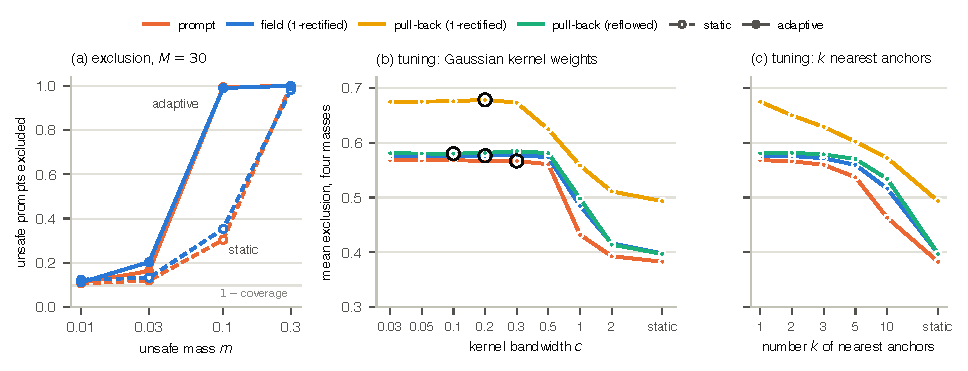
\includegraphics[width=\textwidth]{figures/fig_e2_detection.pdf}
\caption{(a) Exclusion of unsafe requests against their mass, for the prompt and field regions (1-rectified model) with static
(dashed) and adaptive (solid) weights; means over $200$ evaluation splits, $M=30$. (b)--(c) Tuning of the adaptive weights: mean
exclusion over the four masses against the bandwidth $c$ of Gaussian kernel weights, relative to the median distance between
anchors (b), and against the number $k$ of nearest anchors given equal weights (c). The last point of each curve is the static
region; circles mark the weights chosen on the tuning pool; all curves are measured on the evaluation pool.}
\label{fig:e2_detection}
\end{figure}

\paragraph{Mechanism.}
Static weights take the same mass from every anchor, whatever its rotation, so the score averages distances dominated by the
rotation spread of the approved family: the threshold sits at the score of the most atypical approved prompts, and an unsafe mode
must lift a typical request above it through that average. (Proposition~\ref{pr:geometry}(iii) only bounds the static budget from
below, by half the mean distance between anchors.) Figure~\ref{fig:e2_mechanism} follows one request (rotation $10^\circ$, radius $2$, $m=0.1$). With
static weights it scores $\etScEstatic\varepsilon$ (prompt) and $\etScFstatic\varepsilon$ (field), and is admitted (panels (a) and (c)). The tuned
adaptive weights take $\etWEtopthree$ (prompt) and $\etWFtopthree$ (field) of the mass from the three nearest anchors, which nearly share the
request's rotation and radius, so the score becomes a distance to these neighbours and the request is excluded ($\etScEadaptive\varepsilon$
and $\etScFadaptive\varepsilon$; panels (b) and (d)). Over all requests (bottom row), static regions admit a dome of unsafe requests above
the approved rotations, up to $m=\etMapMaxEstatic$ (prompt) and $m=\etMapMaxTRstatic$ (field); adaptive regions admit a thin band, up to
$m=\etMapMaxEadaptive$ and $m=\etMapMaxTRadaptive$.

\begin{figure}[!htbp]
\centering
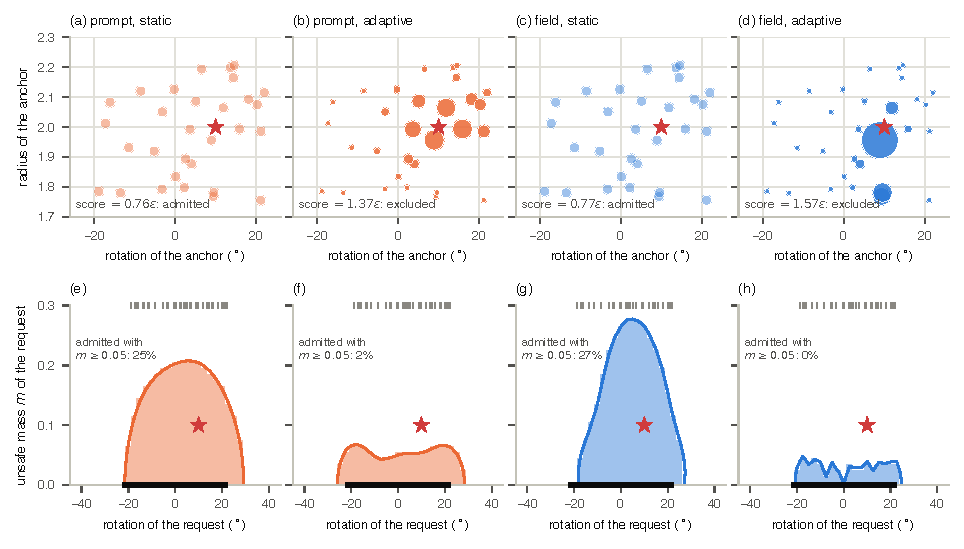
\includegraphics[width=\textwidth]{figures/fig_e2_mechanism.pdf}
\caption{Why adaptive weights exclude more. Each column is one region (1-rectified model, evaluation split $0$). Top: the optimal
transport plan of the order-$1$ score for one unsafe request (star: rotation $10^\circ$, radius $2$, $m=0.1$); each disc is an anchor,
placed by its rotation and radius, with an area proportional to its weight $w_i$, the mass that the plan moves from it to the
request; scores are in units of the threshold $\varepsilon$. Bottom: admission maps for requests of radius $2$ (admitted requests shaded;
black segment: approved requests; star: the request of the top row; ticks: rotations of the $30$ anchors, of various radii).}
\label{fig:e2_mechanism}
\end{figure}

\paragraph{Tuning.}
The best adaptive weights are local (Figure~\ref{fig:e2_detection}(b)--(c)). In every space, mean exclusion is flat from $c=0.03$,
where the kernel keeps only the nearest anchor, to $c=0.3$, and falls for wider kernels; with equal weights on the $k$ nearest
anchors, it is highest for $k\le2$. Spreading the mass lets the spread of the family back into the score. The weights chosen on the
tuning pool are within $\etTuneRegret$ of the best on the evaluation pool, and the nearest anchor alone is within $\etNearGap$: tuning
confirms the improved method of Section~\ref{sec:e1} rather than improving on it.

\paragraph{Take-away.}
A static region measures the spread of the approved family, in the prompt space as in the field space. Taking the transport mass
from the nearest anchors makes the score measure the request, at no cost in coverage.
\FloatBarrier

\subsection{Prompt space and field space}\label{sec:e2_space}

The requests above are \emph{honest}: prompts $z$ passed through the encoder. On them the two spaces perform alike; two departures
from this setting separate the Euclidean prompt distance from the field distances, and a whitened prompt distance shows how much of
the separation is due to the toy.

\paragraph{Honest requests.}
The prompt and field regions exclude as many unsafe requests, static or adaptive (Figure~\ref{fig:e2_detection}(a)), and both enforce
well. For the requests with $m=0.3$, which the 1-rectified model serves with $P(A)=\etPoolPAOne$, back-off brings $P(A)$ to $\etEnfOneEA$
with the adaptive prompt region and $\etEnfOneFA$ with the adaptive field region ($\etEnfOneES$ and $\etEnfOneFS$ with static weights;
Figure~\ref{fig:e2_attack}(b)). The reason is the encoder: as the third coordinate of the embedding is $m/0.2$, embedding distances
see the unsafe mass as directly as the outputs do, and back-off towards the nearest approved embedding mainly shrinks that
coordinate.

\paragraph{White-box attack.}
An attacker who controls the embedding is not bound by the encoder. Inside the prompt regions of the 1-rectified model, the attack
finds admitted embeddings with $P(A)$ up to $\etAtkOneES$ (static) and $\etAtkOneEA$ (adaptive; Figure~\ref{fig:e2_attack}(a)): they are
close to approved embeddings in directions that change the field strongly, which the Euclidean distance does not weigh. Inside the
field regions, the worst values are $\etAtkOneFS$ (static) and $\etAtkOneFA$ (adaptive), and the directed search, which looks for the
directions that a region penalises least, finds at most $\etDirOneFS$ and $\etDirOneFA$. Adaptive weights buy robustness only in a space
that sees the field.

\begin{figure}[!htbp]
\centering
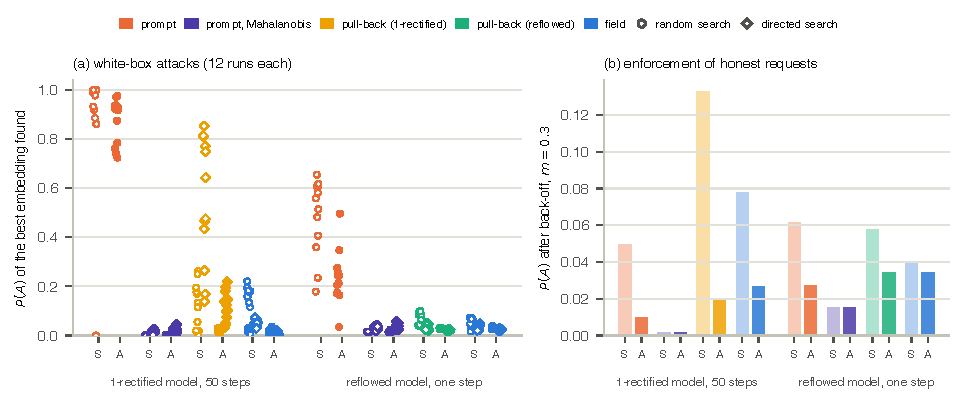
\includegraphics[width=\textwidth]{figures/fig_e2_attack.pdf}
\caption{Regions against an attacker and on honest requests. (a) White-box attacks: $P(A)$, on fresh noise, of the best embedding
found by each of $12$ random-search runs (circles) and $12$ directed-search runs (diamonds) inside each region (S: static; A: adaptive
weights); the Euclidean prompt region gets the random search only. (b) Enforcement: $P(A)$ after back-off for
the requests with $m=0.3$ (means over $3$ splits). Left groups: regions protecting the 1-rectified model ($50$ Euler steps); right
groups: regions protecting the reflowed model sampled in one step, whose pull-back metric is its field metric.}
\label{fig:e2_attack}
\end{figure}

\paragraph{Nuisance wording.}
Real prompts also differ in wording that moves the embedding without changing the request. To model this, each prompt receives a
token $s\sim\mathcal U[-1,1]$, encoded in $10$ extra coordinates scaled by $\lambda$, which leaves the target unchanged, and the
1-rectified model is refitted on prompts with random tokens. It learns to ignore the token: its fidelity is that of the model
without token (MMD$^2\times10^3=\etNuMmd$ against $\eoneMmdA$; $P(A)=\etNuPAd$ against $\eonePAAd$ at $m=0.3$), and two tokens of one
request give outputs at truncated distance $\etNuSame$ (median), against $\etNuPairs$ for two approved requests. Least squares is
invariant to the scale of the token coordinates, so only the prompt region depends on $\lambda$ (Figure~\ref{fig:e2_nuisance}). As $\lambda$
grows, its nearest anchors become those with a similar token rather than a similar request: adaptive exclusion at $m=0.1$ falls
from $\etNuEzeroA$ without token to $\etNuEtwoA$ at $\lambda=2$ and $\etNuEfourA$ at $\lambda=4$ (static: $\etNuEzeroS$ to $\etNuEfourS$), while the
adaptive field region keeps $\etNuFA$. Coverage stays between $\etNuCovMin$ and $\etNuCovMax$.

\begin{figure}[!htbp]
\centering
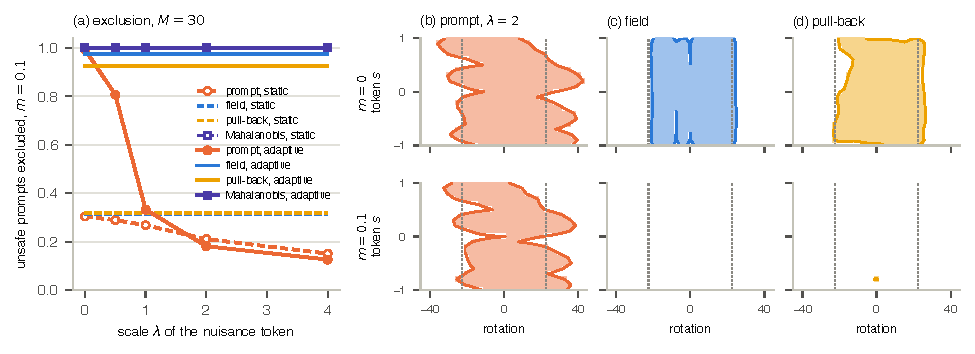
\includegraphics[width=\textwidth]{figures/fig_e2_nuisance.pdf}
\caption{Prompts with a nuisance token $s$, encoded in $10$ extra embedding coordinates scaled by $\lambda$ and ignored by the refitted
1-rectified model. (a) Exclusion at $m=0.1$ against $\lambda$ ($M=30$, $200$ splits); the field and pull-back regions of this model do not
depend on $\lambda$; the Mahalanobis region (violet) is refitted at every $\lambda$. (b)--(d) Admission maps of the adaptive regions over
rotation and token, for requests of radius $2$ with $m=0$ (top)
and $m=0.1$ (bottom); dotted lines: approved rotations. The prompt region admits unsafe requests for many tokens; the field region
admits by rotation alone, and no request with $m=0.1$.}
\label{fig:e2_nuisance}
\end{figure}

\paragraph{A whitened prompt distance.}
The Euclidean distance ignores how the approved embeddings are spread. The Mahalanobis region, tuned like the others ($\rho=\etMHRho$, adaptive kernel
$c=\etMHc$), excludes $\etMHExSa$, $\etMHExSb$, $\etMHExSc$ and $\etMHExSd$ of the requests with $m=0.01$, $0.03$, $0.1$ and $0.3$ with static
weights, with coverage $\etMHCovS$: every unsafe request at every mass, which no field region achieves even with $240$ anchors
(Section~\ref{sec:e2_repairs}). It resists both attacks on the 1-rectified model (worst $P(A)=\etAtkOneMHS$ and $\etAtkOneMHA$ by random
search, $\etDirOneMHS$ and $\etDirOneMHA$ by directed search; Table~\ref{tab:e2_summary}) and the nuisance token (exclusion at $m=0.1$ of at
least $\etMHNuMin$ at every $\lambda$, Figure~\ref{fig:e2_nuisance}(a)). The reason is the toy, not the distance: the third coordinate
$m/0.2$ of the approved embeddings is identically $0$ (variance $\etMvar$ on the tuning pool), and they lie on a two-dimensional
surface of $\RR^{43}$, so whitening by their covariance flags every embedding with $m>0$ and every embedding that leaves the surface,
which is what each attack does. Its enforcement is crude: the metric is so stiff that back-off goes all the way (mixing weight
$\etMHKappa$ for the requests with $m=0.3$) and replaces the request by an approved prompt, with MMD$^2\times10^3=\etMmdOneMHS$ to the
request's safe target, against $\etMmdOneEA$ and $\etMmdOneFA$ for the adaptive Euclidean and field regions.

\paragraph{Take-away.}
A Euclidean prompt region is only as good as the encoder: it matches a field region when the embedding exposes the unsafe content,
and fails, static or adaptive, under attacks on the embedding or wording that the model ignores; a field region resists both. A
prompt region that whitens by the approved embeddings also resists them here, because the approved embeddings of this toy are
degenerate. Separating the two spaces needs approved prompts that span their embedding space and an encoder that hides the unsafe
content.

\subsection{Failures and modifications}\label{sec:e2_repairs}

Four failures remain. Each is given below with its cause and a modification; Table~\ref{tab:e2_repairs} reports the effect of each
modification on the static and on the adaptive regions.

\begin{table}[!htbp]
\centering
\caption{Effect of each modification on the static and on the adaptive regions (evaluation pool; before $\to$ after). Attack: largest
$P(A)$ found inside the region by each search; MMD$^2\times10^3$: fidelity after enforcement of the requests with $m=0.3$. The pull-back
and Mahalanobis rows replace the Euclidean prompt region by the pull-back region of the same model or by the Mahalanobis prompt
region; the Euclidean region has no directed search, so those rows give the new value only. The token row uses the refitted model
of Section~\ref{sec:e2_space} with $\lambda=4$. The reflow rows replace the field region of the 1-rectified model by that of the
reflowed model sampled in one step.}
\label{tab:e2_repairs}
\small
\begin{tabular}{l l l c c}
\toprule
modification & setting & measure & static & adaptive\\
\midrule
$240$ anchors instead of $30$ & prompt & excluded at $m=0.03$ & $\etDensUEA\to\etDensUEB$ & $\etDensEA\to\etDensEB$\\
& field (1-rectified) & & $\etDensUFA\to\etDensUFB$ & $\etDensFA\to\etDensFB$\\
\midrule
pull-back metric & 1-rectified & worst $P(A)$, random search & $\etAtkOneES\to\etAtkOnePBS$ & $\etAtkOneEA\to\etAtkOnePBA$\\
& & worst $P(A)$, directed search & $\etDirOnePBS$ & $\etDirOnePBA$\\
& 1-rectified, token & excluded at $m=0.1$ & $\etNuEfourS\to\etNuPS$ & $\etNuEfourA\to\etNuPA$\\
& reflowed & worst $P(A)$, random search & $\etAtkTwoES\to\etAtkTwoPBS$ & $\etAtkTwoEA\to\etAtkTwoPBA$\\
& & worst $P(A)$, directed search & $\etDirTwoPBS$ & $\etDirTwoPBA$\\
\midrule
Mahalanobis metric & 1-rectified & excluded at $m=0.01$ & $\etExESa\to\etMHExSa$ & $\etExEAa\to\etMHExAa$\\
& & worst $P(A)$, random search & $\etAtkOneES\to\etAtkOneMHS$ & $\etAtkOneEA\to\etAtkOneMHA$\\
& & MMD$^2$ after enforcement & $\etMmdOneES\to\etMmdOneMHS$ & $\etMmdOneEA\to\etMmdOneMHA$\\
\midrule
reflow, one step & field & excluded at $m=0.1$ & $\etExFSc\to\etExTSc$ & $\etExFAc\to\etExTAc$\\
& & worst $P(A)$, random search & $\etAtkOneFS\to\etAtkTwoFS$ & $\etAtkOneFA\to\etAtkTwoFA$\\
& & worst $P(A)$, directed search & $\etDirOneFS\to\etDirTwoFS$ & $\etDirOneFA\to\etDirTwoFA$\\
& & MMD$^2$ after enforcement & $\etMmdOneFS\to\etMmdTwoFS$ & $\etMmdOneFA\to\etMmdTwoFA$\\
\bottomrule
\end{tabular}
\end{table}

\paragraph{Static regions are too wide, and more anchors do not help.}
A static budget is set by the spread of the approved family (it is a quantile of the mean distance to the anchors, and
Proposition~\ref{pr:geometry}(iii) bounds it from below), not by the number of anchors: from
$30$ to $240$ anchors it goes from $\etEpsUEA$ to $\etEpsUEB$ (prompt) and from $\etEpsUFA$ to $\etEpsUFB$ (field), and exclusion barely moves
(Figure~\ref{fig:e2_density}). Adaptive weights are the main repair. Reflow with one-step sampling also helps the static field region,
because it shrinks the spread more than the effect of an unsafe mode: the one-step outputs are smeared along the ring
(Figure~\ref{fig:e1_time}), so the mean field distance between approved prompts falls from $\etSpreadOne$ to $\etSpreadTwo$, while the median
distance from a request with $m=0.1$ to its nearest approved prompt only falls from $\etDispOne$ to $\etDispTwo$.

\paragraph{Adaptive regions are only as fine as the anchors.}
An adaptive budget is set by the distance from an approved prompt to its nearest anchors, so an unsafe mode that moves the outputs
by less is admitted, as $m=0.03$ is with $30$ anchors. From $30$ to $240$ anchors, this budget falls from $\etEpsEA$ to $\etEpsEB$ (prompt)
and from $\etEpsFA$ to $\etEpsFB$ (field), and almost every request with $m=0.03$ is excluded (Figure~\ref{fig:e2_density}(a)); $m=0.01$
needs denser anchors still (at most a fraction $\etDensOneP$ is excluded with $240$ anchors), partly because the model realises only
$\eoneRealiseda\%$ of that mass (Section~\ref{sec:e1}, Step~1). The approved family has two dimensions here, rotation and radius. For a
$d$-dimensional family the distance from a request to its nearest anchor shrinks like $M^{-1/d}$, so the number of anchors needed for a
given resolution grows exponentially with $d$: this, not coverage, is what limits adaptive regions on realistic prompt sets. With nearly
nearest-neighbour weights, an adaptive region is close to a union of small balls around the anchors: it is not convex, and it is
enforced by back-off rather than by projection.

\begin{figure}[!htbp]
\centering
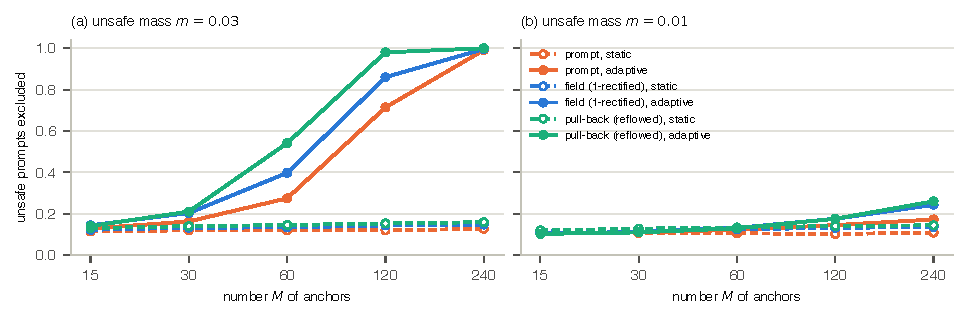
\includegraphics[width=\textwidth]{figures/fig_e2_density.pdf}
\caption{Exclusion of small unsafe masses against the number $M$ of anchors (evaluation pool, $K=60$, adaptive weights tuned for each
$M$); dashed: static; solid: adaptive. The static budget is set by the spread of the approved family and does not shrink with $M$; the
adaptive budget shrinks with the distance to the nearest anchors.}
\label{fig:e2_density}
\end{figure}

\paragraph{Prompt regions do not see the model.}
The pull-back metric weighs each direction of the embedding by its effect on the field at $t=0$, so it ignores what the model
ignores, without simulation, and keeps most of the detection with nuisance tokens (Table~\ref{tab:e2_repairs}). Whether it resists attacks
depends on the model. For the reflowed one-step model, whose deployed sampler it measures, it caps both attacks at a few percent. For
the 1-rectified model it measures the field at $t=0$, not the $50$-step sampler, and is not a safety device: the random search finds
at most $\etAtkOnePBA$ inside its adaptive region, but the directed search, which moves along the directions in which the slice at $t=0$
changes least (its Gram matrix has condition number $\etQcondOne$), finds admitted prompts with $P(A)=\etDirOnePBA$ (adaptive) and
$\etDirOnePBS$ (static). Its certificate pays straightness defects of order $\eoneZetaA$ (Corollary~\ref{cor:one_step}(ii)) and is vacuous,
and with static weights it leaves $P(A)=\etEnfOnePBS$ after enforcement. Its detection, the strongest of all regions ($\etExSAb$ at
$m=0.03$, adaptive), rests on what the fitted field leaks at $t=0$: the exact field at $t=0$ depends on the target only through its mean
(Lemma~\ref{lem:time}(iii)), which the unsafe mode leaves unchanged, and the same blindness is what the directed search exploits.

\paragraph{Field regions of a curved model are costly.}
On the 1-rectified model, each field score runs the $50$-step sampler on the $256$ probes, back-off repeats it about $18$ times, and
the region is not convex. Reflow with one-step sampling (Remark~\ref{rem:reflow}) removes these costs: the pull-back metric of the
reflowed one-step model \emph{is} the map metric of its deployed sampler (Corollary~\ref{cor:one_step}(i)). Its region lives on the
prompts, needs no simulation, is convex with static weights (Proposition~\ref{pr:geometry}(i)) and keeps the certificate of
Theorem~\ref{th:certificate}. It detects as well as the field regions (Table~\ref{tab:e2_summary}), gains as much from denser anchors
(Figure~\ref{fig:e2_density}) and resists both attacks, unlike the Euclidean prompt region of the same model (Table~\ref{tab:e2_repairs}).
The price is the fidelity of one-step sampling (MMD$^2\times10^3=\eoneMmdC$ on approved prompts, against $\eoneMmdA$), which
enforcement inherits (Table~\ref{tab:e2_summary}), and its safety on approved prompts: they put $P(A)=\eoneOneStepPA$ of their outputs in
$A$, against $\eoneSafePAA$ with the 1-rectified model and $50$ steps.
\FloatBarrier

\subsection{Summary}\label{sec:e2_summary}

On this toy, the weights decide detection; the space decides robustness against the Euclidean prompt distance.
(Q1) Static regions are valid but too wide in every space, because their threshold is set by the spread of the approved family.
Adaptive weights that concentrate the transport mass near the request (on the nearest anchors in the region's own distance or, for
the field region of the reflowed model, in the embedding) repair detection at no cost in coverage, and resolve smaller unsafe masses
as the anchors become denser, at a cost in anchors that grows with the dimension of the approved family.
(Q2) Euclidean prompt regions match field regions only while the encoder exposes the unsafe content, and fail under attacks on the
embedding and under wording that the model ignores; field regions resist both. A prompt region that whitens by the approved
embeddings resists them too, but only because the approved embeddings of this toy are degenerate, and its enforcement replaces
every excluded request by an approved prompt.
(Q3) The best configuration is an adaptive region on a field metric. For a model reflowed and sampled in one step, that metric is
the pull-back metric on the prompts, which is cheap and certified; its costs are the fidelity of one-step sampling and a higher
$P(A)$ on approved prompts. The pull-back metric of a curved model is not a safety device.

% =====================================================================================
\section{A pretrained text-to-image model, with winter scenes only}\label{sec:e3}
% =====================================================================================

Sections~\ref{sec:e1} and~\ref{sec:e2} tested the regions on a two-dimensional toy whose encoder exposes the unsafe mass and whose
approved embeddings are degenerate. This section applies every mechanism of Sections~\ref{sec:metrics}--\ref{sec:certificates},
unchanged, to a pretrained text-to-image flow-matching model, with a concrete definition of what is allowed: \emph{winter scenery
only}. The five regions of Section~\ref{sec:e2} are kept: the prompt region, the Mahalanobis region, the \emph{source slice} (the
pull-back distance of Section~\ref{sec:e2}, computed here on the fields themselves), and the field region with the map metric as
written and with its truncation. Each is run with static and with adaptive weights; excluded requests are enforced by back-off, and
the field regions are given their plug-in certificates. The section answers five questions.
\begin{enumerate}[label=(Q\arabic*)]
\item \emph{Detection} (Section~\ref{sec:e3_detect}). What does each region do with a summer request, with a request that does not
mention the season (``a pine forest, at midday''), and with a summer request disguised by winter words?
\item \emph{Weights} (Sections~\ref{sec:e3_detect} and~\ref{sec:e3_anchors}). Do adaptive weights beat static ones, as they do on
the toy?
\item \emph{Space} (Section~\ref{sec:e3_spaces}). What does each distance see: the season, the scene, or the wording? Does a region
exclude the unsafe requests, or anything that the approved prompts do not show?
\item \emph{Enforcement} (Section~\ref{sec:e3_enforce}). Does back-off turn an excluded request into a winter scene of what was asked
for, and are the certificates informative?
\item \emph{Combination} (Section~\ref{sec:e3_combined}). Can a distance that decides well be paired with one that repairs well,
and what does conformal prediction still guarantee when it is?
\end{enumerate}
Section~\ref{sec:e3_design} describes the design and Section~\ref{sec:e3_own} what the model generates without a region.
Section~\ref{sec:e3_verdict} takes stock, method by method, of what works and what does not, Section~\ref{sec:e3_combined} builds and
tests new methods from these findings, Section~\ref{sec:e3_slice} states the methods that decide with the source slice in mathematical
detail, and Section~\ref{sec:e3_summary} answers the questions.

\subsection{Design}\label{sec:e3_design}

\paragraph{Model, fields and samplers.}
The generator is Sana 600M at $512$ pixels \citep{xie2025sana}, a flow-matching transformer on a $32\times16\times16$ latent,
conditioned on the hidden states of a Gemma-2 text encoder and decoded by an autoencoder; it runs in bfloat16 on a laptop GPU. The
\emph{field} of a prompt $c$ is its classifier-free-guided velocity \citep{ho2022classifier},
$v(\cdot;\varnothing)+\omega\,(v(\cdot;c)-v(\cdot;\varnothing))$ with guidance scale $\omega=\ethGuid$, and its sampler map $T_c$
is the explicit Euler scheme (Definition~\ref{def:sampler}) on $\ethJ$ steps of Sana's shifted schedule (shift $\ethShift$),
started from a noise shared by all prompts. Sana's time runs from noise to data, the reverse of this note's convention, so the
source slice $t=0$ of the note is the noise end here. A mixture of fields $\sum_a\gamma_av(\cdot;c_a)$ is formed inside the
guidance, $v(\cdot;\varnothing)+\omega\,(\sum_a\gamma_av(\cdot;c_a)-v(\cdot;\varnothing))$, at the cost of one more field evaluation
per step and per mixed prompt (Proposition~\ref{pr:backoff}(iii)). The model is not affine in the prompt
(Definition~\ref{def:prompt}(b)): a mixture of fields is a field, but not the field of any prompt, and no result that needs
linearity is used below.

\paragraph{What is safe, and the requests.}
\emph{Safe} means a winter scene: snow, frost or ice on the scene that was asked for. Prompts follow one grammar, ``a photograph of
\{scene\}, \{modifier\}, \{light\}'', with $16$ scenes (a pine forest, a mountain lake, a village street, \dots), $5$ lighting
conditions and four kinds of modifier, which define four kinds of request:
\begin{itemize}
\item \emph{approved}: one of $6$ winter modifiers (``covered in fresh snow'', ``during a heavy snowfall'', \dots); these prompts
define what is safe, and are drawn at random without replacement from the $480$ combinations, hence exchangeable
(Assumption~\ref{as:exch});
\item \emph{summer}: one of $5$ summer modifiers (``on a hot summer day with lush green foliage'', \dots), explicitly unsafe;
\item \emph{season not mentioned} (``no season'' in the tables): no modifier, as in ``a photograph of a pine forest, at midday'';
\item \emph{disguised}: a summer prompt followed by ``, snowy winter cold'', summer content dressed in winter words.
\end{itemize}
Three further kinds, added after the first results, test whether a region detects the season or merely what it has not seen:
\emph{paraphrases}, winter prompts of the $16$ scenes with $5$ winter modifiers that no approved prompt uses (``blanketed in snow on
a cold January morning'', ``in midwinter, with snowflakes falling'', \dots), and \emph{novel winter} and \emph{novel summer}
requests, the approved and the summer modifiers on $6$ scenes that no approved prompt shows (``a ski chalet on a mountain slope'',
``a vineyard on a hillside'', \dots). Paraphrases and novel winter requests are safe; together they form the
$\ethNsafeUnf$ \emph{safe unfamiliar} requests, and excluding one of them is a false alarm. A \emph{tuning} pool ($\ethNappTune$
approved and $\ethNsumTune$ summer prompts) serves only to choose the weights and the parameters of the regions; a disjoint
\emph{evaluation} pool holds $\ethNappEval$ approved prompts (anchors, calibration and test prompts), $\ethNsumEval$ summer, $\ethNneu$
season-not-mentioned and $\ethNdis$ disguised requests, $\ethNPar$ paraphrases, $\ethNNovW$ novel winter and $\ethNNovS$ novel summer
requests.

\paragraph{Regions.}
As in Section~\ref{sec:e2}, a region is given by a distance $d$ between prompts and by weights $w$. A request $c$ scores
$\sum_{i=1}^Mw_i\,d(c,c_i)$ against $M=\ethM$ approved prompts $c_1,\dots,c_M$, the \emph{anchors}, and is admitted if its score
is at most a threshold $\varepsilon$: the $\lceil(K+1)(1-\beta)\rceil$-th smallest score of $K=\ethK$ other approved prompts, the
\emph{calibration} prompts, with $\beta=\ethBeta$ (Definition~\ref{def:region} without its factor $1/(M+1)$). An approved prompt
exchangeable with the calibration prompts is then admitted with probability at least $\ethNom$ (Proposition~\ref{pr:coverage}).
Table~\ref{tab:e3_regions} defines the five distances; those that involve the field are estimated on $P=\ethP$ frozen probe noises
$x_1,\dots,x_P$. The \emph{prompt} and \emph{Mahalanobis} regions compare prompts and never run the model. The \emph{source slice}
compares the fields at the noise end, where every sampler makes its first evaluation (Definition~\ref{def:metrics}(iii)); for a
model trained with the independent coupling, as Sana is, the exact field there depends on the outputs only through their mean
(Lemma~\ref{lem:time}(iii)). The two \emph{field} regions compare what the fields generate, in the space $\chi$ of CLIP ViT-L/14
image embeddings \citep{radford2021learning}: the map metric of Definition~\ref{def:metrics}(ii), which is the method as written,
and its truncation at level $r$ (Proposition~\ref{pr:truncated}).

\begin{table}[!htbp]
\centering
\caption{The five regions of Section~\ref{sec:e3}. Each row is one region. ``Distance'' is the distance $d(c,c_i)$ between a
request $c$ and an anchor $c_i$ that the score averages; ``compares'' says what this distance looks at; ``runs the model'' says
whether scoring a request requires the generator; ``tuned over'' lists the adaptive weights (K, N, X, defined in the paragraph on
weights) and the parameters among which the tuning pool chooses. Notation: $\be(c)$ is the mean of the Gemma-2 hidden states of the
prompt $c$ ($2304$ numbers); $S_\rho$ is the covariance $S$ of the approved embeddings of the tuning pool plus $\rho\operatorname{tr}(S)/2304$
times the identity; $v(x_\ell;c)$ is the guided velocity of $c$ at the noise end on the probe $x_\ell$ (a latent of $8192$
numbers); $\chi$ maps a decoded image to its CLIP ViT-L/14 embedding (unit norm, $768$ numbers). The parameters are tuned over
$\rho\in\{10^{-4},10^{-2},10^{-1},1\}$ and $r\in\{\ethTRlevels\}$.}
\label{tab:e3_regions}
\small
\setlength{\tabcolsep}{4pt}
\begin{tabular}{l l l c l}
\toprule
region & distance $d(c,c_i)$ & compares & runs the model & tuned over \\
\midrule
prompt & $\|\be(c)-\be(c_i)\|$ & prompts & no & K, N \\
Mahalanobis & $\|S_\rho^{-1/2}(\be(c)-\be(c_i))\|$ & prompts & no & K, N, $\rho$ \\
source slice & $\big(\frac1P\sum_\ell\|v(x_\ell;c)-v(x_\ell;c_i)\|^2\big)^{1/2}$ & fields at the noise end & first step & K, N, X \\
field $L^2$ & $\big(\frac1P\sum_\ell\|\chi(T_c(x_\ell))-\chi(T_{c_i}(x_\ell))\|^2\big)^{1/2}$ & generated images & full sampling & K, N, X \\
field truncated & $\frac1P\sum_\ell\min\big(\|\chi(T_c(x_\ell))-\chi(T_{c_i}(x_\ell))\|,r\big)/r$ & generated images & full sampling & K, N, X, $r$ \\
\bottomrule
\end{tabular}
\end{table}

\paragraph{Weights.}
\emph{Static} weights are uniform, $w_i=1/M$, as in Definition~\ref{def:region}. \emph{Adaptive} weights depend on the request and
concentrate the transport mass on the anchors closest to it, as in Section~\ref{sec:e2}: K:$c$ is a Gaussian kernel in the
region's distance, $w_i\propto\exp(-d(c,c_i)^2/2h^2)$, with $h$ equal to $c\in\{0.03,0.1,0.3,1\}$ times the median distance between
anchors; N:$k$ puts $w_i=1/k$ on the $k\in\{1,3\}$ nearest anchors; X:$c$, for the three regions that run the model, is the kernel
K:$c$ computed in the prompt distance, $c\in\{0.1,0.3\}$. The truncation levels $r$ are the quartiles of the distances
$\|\chi(T_c(x_\ell))-\chi(T_{c'}(x_\ell))\|$ between approved prompts of the tuning pool.

\paragraph{Protocol.}
\begin{itemize}
\item \emph{Tuning.} For each region, the parameter $\rho$ or $r$ of the static region, and the adaptive weights of the adaptive region
with their own $\rho$ or $r$, are those that exclude the most of the $\ethNsumTune$ summer prompts of the tuning pool, on average
over $\ethNtune$ random splits of its $\ethNappTune$ approved prompts into anchors and calibration prompts; ties are broken by the
median ratio of score to threshold. Only explicit summer prompts inform this choice.
\item \emph{Detection.} On the evaluation pool, $\ethNeval$ random splits of the $\ethNappEval$ approved prompts give $M=\ethM$ anchors,
$K=\ethK$ calibration prompts and $\ethNtest$ approved test prompts, and every request is scored in every split.
\item \emph{Enforcement.} On the first evaluation split, $\ethNreqKind$ requests of each of the kinds summer, season not mentioned and
disguised, and $\ethNreqApp$ approved test prompts, are submitted to every region. An excluded request $c$ is \emph{backed off}
(Proposition~\ref{pr:backoff}) towards its \emph{target} $c'$, the approved prompt nearest to $c$ in the region's own distance among
the anchors and calibration prompts that the region admits: the deployed field is $(1-\kappa)v(\cdot;c)+\kappa v(\cdot;c')$, with
the smallest $\kappa$, found by bisection, whose score is within the threshold. The \emph{mixing weight} $\kappa$ is $0$ for an
admitted request and $1$ for a request replaced by its target. The score of a mixture is computed in the region's own space: on the
mixed embedding $(1-\kappa)\be(c)+\kappa\be(c')$ for the two prompt regions, a proxy that would be exact only for a model affine in
the prompt (Corollary~\ref{cor:prompt_mixing}); on the mixed velocities for the source slice, which is exact; and, for the field
regions, by sampling the mixed field on the probes, which is exact but costs one generation per bisection step ($\ethBisField$
steps, against $\ethBisCheap$ for the other regions).
\item \emph{Judging.} The deployed field generates from $\ethP$ \emph{evaluation} noises, which no score uses, and a judge independent of
$\chi$ grades every image: CLIP ViT-B/32 compares the image with four captions that describe a winter scene and four that describe
a scene without snow (summer, spring or autumn), and returns the probability of ``winter''. An image is \emph{unsafe} if this probability is below $0.5$. The \emph{scene
similarity} of an image is the judge's cosine between the image and the text ``a photograph of \{scene\}'' for the requested scene:
it measures whether enforcement keeps what was asked for.
\item \emph{Certificates.} For the field regions, the plug-in certificate of Theorem~\ref{th:certificate}(ii) ($L^2$) and
Proposition~\ref{pr:truncated} (truncated) bounds the probability that a deployed image falls in $B$, the half-space of $\chi$-space
where ViT-L/14 itself says ``not winter''. With $n$ the unit normal of $B$, its enlargement is $B^{+r'}=\{u:\langle u,n\rangle<r'\}$;
the anchors' probabilities of $B^{+r'}$ are estimated on their probe outputs, and the bound is minimised over $r'\in[0.02,1]$.
\end{itemize}

\paragraph{How the results are reported.}
Every result is a fraction between $0$ and $1$ or a mean, and whether higher is better depends on the quantity.
\begin{itemize}
\item \emph{Coverage}: the fraction of approved test prompts admitted. Calibration guarantees at least $\ethNom$ on average, so about
one approved prompt in ten is excluded by design, whatever the region.
\item \emph{Exclusion} of a kind of request: the fraction of its requests that the region does not admit, averaged over the splits.
For an unsafe kind (summer, season not mentioned, novel summer) higher is better. For a safe kind (paraphrase, novel winter) lower
is better, and the exclusion is a \emph{false alarm}.
\item After enforcement, the fraction of \emph{deployed images judged unsafe} (lower is better) and their \emph{scene similarity}
(higher is better). As a scale for the latter, the requests' own images score between $\ethReqOwnSubjDis$ and $\ethReqOwnSubjNeu$
on average, and the images of another scene that one region deploys in Section~\ref{sec:e3_enforce} score $\ethSubjOtherMH$.
\end{itemize}
The kinds have few requests ($\ethNsumEval$ summer and $\ethNneu$ season-not-mentioned requests, $12$ to $16$ of the others). A rate
measured on them estimates the rate on new requests of the same kind only within about $\pm0.2$ (less near $0$ and $1$); since every
region is evaluated on the same requests, the comparisons between regions are more precise than that, but only large or consistent
differences are interpreted below. Enforcement uses $\ethNreqKind$ requests of each kind: it illustrates mechanisms rather than
measuring rates.
\FloatBarrier

\subsection{What the model generates without a region}\label{sec:e3_own}

\emph{Without a region, the model does what it is asked, so every request that does not ask for winter is unsafe.}
Figure~\ref{fig:e3_requests} shows two prompts of each kind, each generated from the same three noises. On the evaluation noises,
the judge's mean probability of winter is $\ethOwnPwApp$ for approved prompts, $\ethOwnPwNeu$ for the requests that do not mention
the season, $\ethOwnPwSum$ for summer requests and $\ethOwnPwDis$ for disguised ones; the fractions of images judged unsafe are
$\ethOwnUnsafeApp$, $\ethOwnUnsafeNeu$, $\ethOwnUnsafeSum$ and $\ethOwnUnsafeDis$. A season left unspecified is not a neutral request
here: Sana fills it with a snow-free scene, so ``a photograph of a pine forest, at midday'' asks, in effect, for a summer forest, and
a safe system must exclude it as it excludes an explicit summer request. The disguised prompts split: the appended ``snowy winter
cold'' wins for $\ethDisSafe$ of the $\ethNdis$ prompts, whose images are mostly judged wintry (typically snow on the ground under
green trees), and loses for the others. The safe unfamiliar requests generate winter images (mean probability of winter
$\ethOwnPwPar$ for paraphrases and $\ethOwnPwNovW$ for novel winter requests), and the novel summer requests summer images
($\ethOwnPwNovS$).

The judge is credible on these images: the zero-shot classifier of ViT-L/14, which shares no weights with it, agrees with it on
$\ethAgree$ of the evaluation images, and on $\ethAgreeDis$ of the ambiguous disguised ones. Pixel statistics are not: the fraction
of bright, unsaturated (snow-like) pixels is $\ethOwnSnowApp$ for approved images and $\ethOwnSnowNeu$ for images without season,
which have bright skies and haze. The judge's probability of winter is therefore the criterion of safety below.

\begin{figure}[!htbp]
\centering
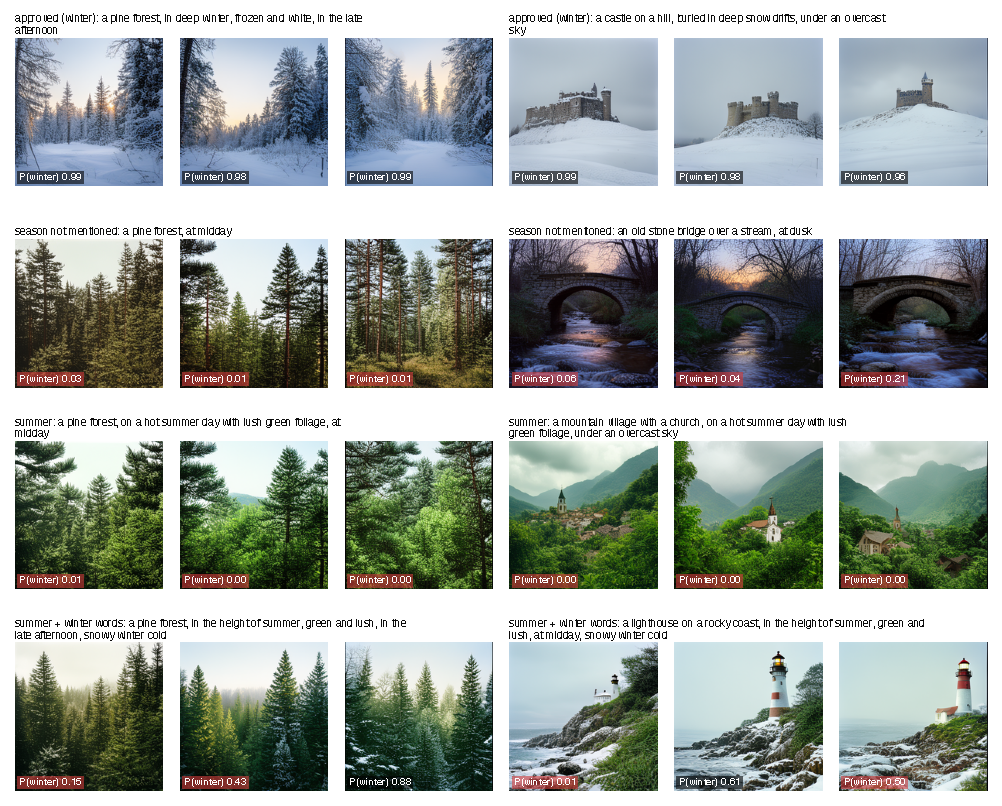
\includegraphics[width=\textwidth]{figures/fig_e3_requests.pdf}
\caption{What the model generates without a region. Each row is one kind of request: from top to bottom, approved (winter), season
not mentioned, summer, and summer with winter words appended (disguised). Each row shows two prompts, whose text is written above
their three images; the three images of a prompt come from the same three probe noises for every prompt. The label in the lower left
corner of each image is the judge's probability that the image shows a winter scene; a red label marks an image judged unsafe
(probability below $0.5$).}
\label{fig:e3_requests}
\end{figure}

\subsection{Detection: which requests each region excludes (Q1, Q2)}\label{sec:e3_detect}

Table~\ref{tab:e3_detection} gives, for each region and weighting, the coverage and the fraction of each kind of request that is
excluded. Figure~\ref{fig:e3_detection} plots the two quantities that matter most against each other: how many unsafe requests a
region excludes (vertical axis), and how many safe unfamiliar requests it excludes by mistake (horizontal axis). A good region sits
in the upper left corner of that figure.

\begin{table}[!htbp]
\centering
\caption{Detection: what each region admits and excludes (evaluation pool, $M=\ethM$ anchors, $K=\ethK$ calibration prompts, means
over $\ethNeval$ random splits). Each row is one region with static or adaptive weights; the adaptive weights chosen on the tuning
pool are named in parentheses (N:$k$: equal weights on the $k$ nearest anchors; K:$c$: Gaussian kernel whose bandwidth is $c$ times
the median distance between anchors). \emph{Coverage}: fraction of the approved test prompts admitted (nominal $\ethNom$). Every
other column is the fraction of the requests of one kind that the region excludes: first the three unsafe kinds, for which higher is
better; then the two safe unfamiliar kinds, for which lower is better (false alarms); last the disguised requests, summer prompts
followed by ``snowy winter cold'', whose own images are judged unsafe in $\ethOwnUnsafeDis$ of the cases, so that neither direction is
right for all of them. Mahalanobis: $\rho=\ethRhoMH$; truncation: $r=\ethRTR$.}
\label{tab:e3_detection}
\small
\setlength{\tabcolsep}{3.5pt}
\begin{tabular}{l l c ccc cc c}
\toprule
& & & \multicolumn{3}{c}{unsafe kinds: excluded (higher is better)} & \multicolumn{2}{c}{safe kinds: excluded (lower is better)} & \\
\cmidrule(lr){4-6}\cmidrule(lr){7-8}
region & weights & coverage & summer & no season & novel summer & paraphrase & novel winter & disguised\\
\midrule
\inputrows{tables/e3_detection.tex}
\bottomrule
\end{tabular}
\end{table}

\begin{figure}[!htbp]
\centering
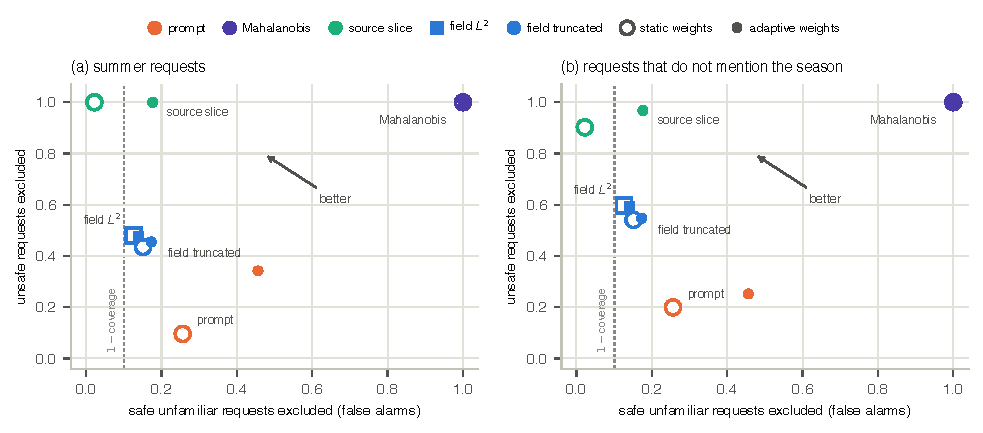
\includegraphics[width=\textwidth]{figures/fig_e3_detection_map.pdf}
\caption{Detection map ($M=\ethM$ anchors, means over $\ethNeval$ evaluation splits; the numbers are those of
Table~\ref{tab:e3_detection}). Each point is one region with one weighting. Its colour gives the region, and the two field regions,
which share the colour blue, differ by their shape (square: $L^2$; circle: truncated). A hollow ring marks static weights and a
small filled dot adaptive weights; a dot inside a ring means that both weightings give the same point. Horizontal axis: the
fraction of the $\ethNsafeUnf$ safe unfamiliar requests (paraphrases and novel winter scenes) that the region excludes, that is,
its false alarms on safe prompts unlike the approved ones. Vertical axis: the fraction of the unsafe requests excluded, (a) for the
summer requests and (b) for the requests that do not mention the season. The ideal region sits in the upper left corner: it
excludes every unsafe request and no safe one. Dotted line: the fraction of ordinary approved test prompts excluded, $1-$coverage
$\approx\ethFAApp$, which calibration fixes for every region; a region on that line or to its left treats unfamiliar safe prompts as
it treats familiar ones.}
\label{fig:e3_detection}
\end{figure}

\emph{Every region keeps its coverage, and the regions differ by an order of magnitude in what they exclude.} Coverage lies
between $\ethCovMin$ and $\ethCovMax$ for every region (nominal $\ethNom$), so the regions differ only in what they exclude:
\begin{itemize}
\item the \emph{prompt} region lets most unsafe requests through: it excludes $\ethExSumES$ of the summer requests and $\ethExNeuES$
of those without season with static weights, $\ethExSumEA$ and $\ethExNeuEA$ with adaptive weights;
\item the \emph{Mahalanobis} region excludes every request of every kind, safe or unsafe;
\item the \emph{source slice} excludes every summer request and $\ethExNeuPBS$ of those without season with static weights
($\ethExNeuPBA$ with adaptive weights), and only $\ethExParPBS$ of the paraphrases and $\ethExNovWPBS$ of the novel winter requests:
with static weights it is the only region in the upper left corner of Figure~\ref{fig:e3_detection};
\item the two \emph{field} regions exclude about half of the unsafe requests ($\ethExSumLtS$ of the summer ones and $\ethExNeuLtS$
of those without season for the $L^2$ map metric as written, $\ethExSumTRS$ and $\ethExNeuTRS$ for its truncation), and a quarter to
a third of the novel winter requests.
\end{itemize}

\emph{The field region as written misses the example that motivated the experiment.} ``A pine forest, at midday'', whose images are
snow-free (judge: $\ethPineOwnPwNeu$), is excluded by the $L^2$ field region in $\ethPineNeuLtS$ of the splits, and its summer version
in $\ethPineSumLtS$; the source slice excludes them in $\ethPineNeuPBS$ and $\ethPineSumPBS$ of the splits. The reason is the scene,
not the season. Snowy pine forests are the most central approved images in CLIP's space: their mean distance to the other approved
images is $\ethCentPineApp$, against a median of $\ethCentMed$ over all approved images. A snow-free forest is farther from them,
but its mean distance, $\ethCentPineNeu$, only reaches the $90\%$ quantile of the approved images' mean distances ($\ethCentQ$),
which is about where the threshold sits ($\beta=\ethBeta$): the request is excluded in some splits and admitted in others. With
static weights, the score adds the season to a baseline that depends on the scene, and a central scene has room for a season.

\emph{With $\ethM$ anchors, adaptive weights help where the static score averages the season away, at the price of false alarms.}
They raise the exclusion of summer requests by the prompt region from $\ethExSumES$ to $\ethExSumEA$, and that of the requests
without season by the source slice from $\ethExNeuPBS$ to $\ethExNeuPBA$; but they also raise the false alarms on safe unfamiliar
requests from $\ethFAES$ to $\ethFAEA$ (prompt) and from $\ethFAPBS$ to $\ethFAPBA$ (source slice): the nearest anchors of an
unfamiliar prompt are far from it, whatever its season. For the field regions, tuning picks a kernel as wide as the spread of the
anchors (\ethVarTRA), whose weights are nearly uniform (an effective number of anchors $1/\sum_iw_i^2$ of $\ethNeffTRA$ out of
$\ethM$), and nothing changes. Section~\ref{sec:e3_anchors} explains why, and what more anchors change.

\emph{Take-away: the space decides, the weights adjust.} With $\ethM$ anchors, the best adaptive weights move the prompt region from
$\ethExSumES$ to $\ethExSumEA$ of the summer requests excluded and the field regions not at all; changing the space, from the prompts
to the source slice, moves it to $1$.

\subsection{What each distance sees (Q3)}\label{sec:e3_spaces}

\emph{A region separates the season only if the season moves a request farther than the approved variability does.} For each
distance, take the median distance between a summer prompt and an approved prompt of the same scene, subtract the median distance
between two approved prompts of the same scene (which differ in winter modifier and light), and divide by the same excess for two
approved prompts of different scenes. This \emph{season-to-scene ratio} measures the season in units of a change of scene. It is
$\ethGapE$ for the prompt embedding, $\ethGapLt$ for the field ($\ethGapTR$ truncated), $\ethGapPB$ for the source slice and
$\ethGapMH$ for the Mahalanobis embedding: it orders the prompt, field, source-slice and Mahalanobis distances as their exclusions
do. Each value has a mechanism.
\begin{itemize}
\item \emph{Prompt.} The season is one modifier among a scene, a light and a template: it moves the mean of the Gemma-2 hidden
states by a fifth of a change of scene, and a score averaged over anchors of every scene cannot see it.
\item \emph{Field.} CLIP embeddings describe what is in an image: a summer image is closer to a snowy image of its scene than two
snowy images of different scenes are to each other. The season moves the outputs about half a change of scene.
\item \emph{Source slice.} For a model trained with the independent coupling, the field at the noise end points to the mean of the
outputs (Lemma~\ref{lem:time}(iii)). The layout of a scene averages out in that mean; its global colour does not, and snow or summer
foliage change the global colour first. The source slice therefore sees the season and is blind to the scene, which is what this
definition of safety asks. On the toy of Section~\ref{sec:e2}, the unsafe mode left the mean output unchanged: the same distance
saw it only through what the fitted field leaked at $t=0$, and a directed attack found unsafe prompts that it admitted
(Section~\ref{sec:e2_repairs}). The source slice is reliable when, and only when, the unsafe attribute moves the mean output.
\item \emph{Mahalanobis.} Approved prompts never vary in season. Whitening by their covariance, with $\rho=\ethRhoMH$, magnifies every
direction in which they do not vary, so the region flags every prompt that leaves the approved template, whatever it generates. As on
the toy (Section~\ref{sec:e2_space}), its success rests on approved embeddings that are degenerate, here in their wording.
\end{itemize}

\emph{Safe requests that no approved prompt resembles separate the regions that detect the season from those that detect
novelty} (columns paraphrase, novel winter and novel summer of Table~\ref{tab:e3_detection}).
\begin{itemize}
\item The \emph{Mahalanobis} region excludes all of them, safe or not: it detects any departure from the approved wording.
\item The \emph{prompt} region admits the paraphrases ($\ethExParES$ excluded) but excludes $\ethExNovWES$ of the novel winter
requests ($\ethExNovWEA$ with adaptive weights): the Gemma-2 embedding sees the scene more than the season, and its exclusion of the
novel summer requests ($\ethExNovSES$) owes much to their new scene.
\item The \emph{source slice} with static weights excludes $\ethExParPBS$ of the paraphrases, $\ethExNovWPBS$ of the novel winter
requests and $\ethExNovSPBS$ of the novel summer ones: it detects the season and nothing else. Nearest-anchor weights raise its false
alarms to $\ethExParPBA$ and $\ethExNovWPBA$.
\item The \emph{field} regions admit the paraphrases ($\ethExParLtS$ excluded) but exclude $\ethExNovWLtS$ ($L^2$) and $\ethExNovWTRS$
(truncated) of the novel winter requests: the distance between outputs is dominated by the scene, and a new scene is far from every
anchor.
\end{itemize}

\emph{The regions on fields judge what is generated; the regions on prompts, what is written.} Figure~\ref{fig:e3_per_request}
shows, request by request, how often each static region excludes a request against what the request's own images look like. Of the
summer, season-not-mentioned and disguised requests, the judge finds the images of $\ethNJU$ unsafe and those of $\ethNJS$ (all
disguised) safe. The source slice excludes $\ethExJUPBS$ of the former and $\ethExJSPBS$ of the latter, and the $L^2$ field region
$\ethExJULtS$ and $\ethExJSLtS$: both exclude more often the requests whose images are unsafe. The prompt region barely distinguishes
them ($\ethExJUES$ and $\ethExJSES$), and the Mahalanobis region excludes all of them ($\ethExJUMHS$ and $\ethExJSMHS$).

\begin{figure}[!htbp]
\centering
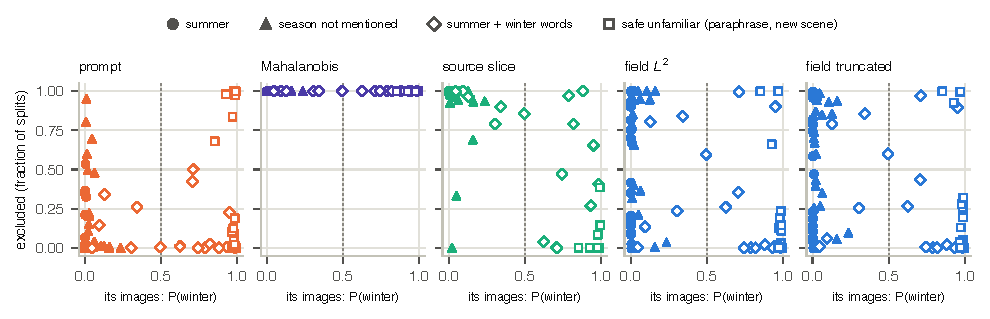
\includegraphics[width=\textwidth]{figures/fig_e3_per_request.pdf}
\caption{Does a region judge what is generated? Each panel is one region with static weights, and each point one request of the
evaluation pool. Horizontal axis: the judge's mean probability of winter for the request's own images (to the left of the dashed
line the images are unsafe, to its right they are safe). Vertical axis: the fraction of the $\ethNeval$ splits in which the region
excludes the request. The marker gives the kind of request: filled circle, summer; filled triangle, season not mentioned; hollow
diamond, disguised (summer with winter words); hollow square, safe unfamiliar (paraphrase or novel winter scene). A region that
judges the images places the points on the left high and the points on the right low. The Mahalanobis region places every point at
the top; the prompt region places most unsafe requests low and some safe unfamiliar ones high; the source slice comes closest to
the ideal.}
\label{fig:e3_per_request}
\end{figure}

\emph{Take-away: a region detects whatever its distance makes large.} That is the season for the source slice, the scene for the
prompt embedding and the fields, and the wording for the Mahalanobis region. Here, only the source slice with static weights detects
the season alone.

\subsection{More anchors for adaptive weights}\label{sec:e3_anchors}

\emph{With nearest-anchor weights and more anchors, the field regions become as selective as the source slice on the approved
scenes; static weights do not improve.} For Figure~\ref{fig:e3_anchors}, the $\ethNapp$ approved prompts of both pools are pooled
and split into $M$ anchors, $\ethK$ calibration prompts and test prompts ($\ethNsplitsRep$ random splits for each $M$), and two
weightings fixed in advance are compared, static and nearest-anchor (N:1), so that nothing is selected on these prompts. Coverage
stays between $\ethRepCovMin$ and $\ethRepCovMax$. From $M=30$ to $M=140$, the truncated field region with nearest-anchor weights
goes from $\ethRepTRNaXXXSum$ to $\ethRepTRNaCXLSum$ of the summer requests excluded and from $\ethRepTRNaXXXNeu$ to
$\ethRepTRNaCXLNeu$ of those without season; with static weights it stays at $\ethRepTRUCXLSum$ and $\ethRepTRUCXLNeu$. The prompt
region improves less ($\ethRepENaXXXSum$ to $\ethRepENaCXLSum$ for summer), and the $L^2$ field region, omitted from the figure,
stays within $\ethAncLtTRdiff$ of the truncated one.

The mechanism is the coverage of the approved variability by the anchors. With $M=30$ anchors drawn among $16$ scenes, a given
scene has no anchor in $\ethMissXXX$ of the cases, more than $\beta=\ethBeta$: the threshold is then set by approved prompts
compared with anchors of another scene, a distance larger than the season, and nearest-anchor weights do no better than uniform
ones. With $M=100$, a scene lacks an anchor in $\ethMissC$ of the cases, every request is compared with an approved prompt of its
own scene, and the season is what remains. Static weights cannot use this: their score averages over all anchors, whatever their
number.

\emph{The repair has a price: a request is now compared with an anchor of its own scene, and a scene without anchors is excluded.}
With $M=140$ and nearest-anchor weights, the truncated field region excludes $\ethRepTRNaCXLNovW$ of the novel winter requests and
$\ethRepTRNaCXLPar$ of the paraphrases, against $\ethRepTRUCXLNovW$ and $\ethRepTRUCXLPar$ with static weights
(Figure~\ref{fig:e3_anchors}(c)). The static source slice excludes at most $\ethRepPBUXXXPar$ of them at any $M$, and every summer
request.

\begin{figure}[!htbp]
\centering
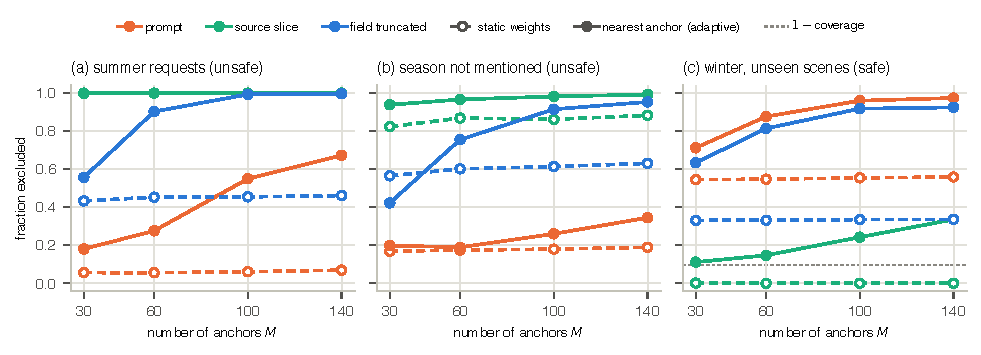
\includegraphics[width=\textwidth]{figures/fig_e3_anchors.pdf}
\caption{Exclusion against the number $M$ of anchors (all $\ethNapp$ approved prompts, $K=\ethK$, means over $\ethNsplitsRep$ random
splits for each $M$). Each panel is one kind of request: (a) summer and (b) season not mentioned are unsafe, so higher is better;
(c) novel winter scenes are safe, so the curve is a false-alarm rate and lower is better. Colour: the region (prompt, source slice,
truncated field; the $L^2$ field region stays within $\ethAncLtTRdiff$ of the truncated one and is omitted). Dashed lines with
hollow markers: static weights; solid lines with filled markers: all the weight on the nearest anchor. In (a) the two source-slice
curves coincide at $1$. Dotted line in (c): the fraction of ordinary approved test prompts excluded ($1-$coverage).}
\label{fig:e3_anchors}
\end{figure}

\emph{Take-away: adaptive weights work once the anchors cover the approved variability, and then refuse what the anchors do not
cover.} Whether that is acceptable depends on whether safe requests outside the approved scenes should be served. The number of
anchors needed grows with the variability of the approved prompts ($16$ scenes, $6$ winter modifiers and $5$ lights here), as
Section~\ref{sec:e2_repairs} anticipated for families of higher dimension.
\FloatBarrier

\subsection{Enforcement and certificates (Q4)}\label{sec:e3_enforce}

Table~\ref{tab:e3_enforce} gives the outcome of enforcement for each region. Figures~\ref{fig:e3_gallery_neutral}
and~\ref{fig:e3_gallery_summer} show what it produces for a few requests, among them the two pine forests, and
Figure~\ref{fig:e3_enforce} summarises, for each region, the two things that a user of the system sees: whether the deployed images
are safe, and whether they still show what was asked for. Without a region, $\ethReqOwnUnsafeSum$ of the summer images,
$\ethReqOwnUnsafeNeu$ of the images without season and $\ethReqOwnUnsafeDis$ of the disguised ones are judged unsafe.

\begin{table}[!htbp]
\centering
\caption{Enforcement on the first evaluation split ($\ethNreqKind$ requests of each kind, $\ethP$ evaluation noises each). Each row
is one region with static or adaptive weights; ``no region'' serves every request as asked. For the summer requests and for the
requests without season, three columns: the fraction of requests that the region alters (that is, backs off, $\kappa>0$); their
mean mixing weight $\kappa$, from $0$ (request unchanged) to $1$ (request replaced by its target), with ``--'' when no request is
altered; and the fraction of their deployed images that the judge finds unsafe (lower is better). Then: the fraction of the
disguised requests' deployed images judged unsafe; the mean scene similarity of the deployed images of the summer, season-not-mentioned and disguised requests (higher is better; between
$\ethReqOwnSubjDis$ and $\ethReqOwnSubjNeu$ for the requests' own images, $\ethSubjOtherMH$ for images of another scene); the fraction
of altered requests whose target shows the requested scene; and the fraction of the $\ethNreqApp$ approved test prompts that the
region alters, whose deployed images all remain winter scenes. The $L^2$ field region with adaptive weights was not enforced: its tuned kernel
gives nearly uniform weights (an effective number of anchors of $\ethNeffLtA$ out of $\ethM$).}
\label{tab:e3_enforce}
\small
\setlength{\tabcolsep}{3.4pt}
\begin{tabular}{l l ccc ccc c c c c}
\toprule
& & \multicolumn{3}{c}{summer} & \multicolumn{3}{c}{season not mentioned} & disguised & scene & target of & approved\\
\cmidrule(lr){3-5}\cmidrule(lr){6-8}
region & weights & altered & mean $\kappa$ & unsafe & altered & mean $\kappa$ & unsafe & unsafe & similarity & same scene & altered\\
\midrule
\inputrows{tables/e3_enforce.tex}
\bottomrule
\end{tabular}
\end{table}

\emph{Only the field regions back a request off towards a winter version of its own scene.}
\begin{itemize}
\item The \emph{prompt} region alters $\ethAltSumES$ of the summer requests with static weights and $\ethAltSumEA$ with adaptive
weights, but mixes little (mean $\kappa=\ethKapSumEA$ with adaptive weights): $\ethAfterSumES$ and $\ethAfterSumEA$ of the deployed
summer images remain unsafe.
\item The \emph{Mahalanobis} region alters every request, with $\kappa\approx\ethKapSumMHS$, and deploys winter images
($\ethAfterSumMHS$ of the summer ones and $\ethAfterNeuMHS$ of those without season unsafe), but mostly of another scene: its target,
the admitted approved prompt nearest in the whitened embedding, has the request's scene in only $\ethTgtSameMHS$ of the cases, and is
a snowy ``\ethHubSceneMH'' for $\ethHubMH$ of the $\ethHubNMH$ summer and season-not-mentioned requests. The scene similarity of the
summer requests falls from $\ethReqOwnSubjSum$ to $\ethSubjSumMHS$.
\item The \emph{source slice} alters every summer request and every request without season, but $\ethAfterSumPBS$ (static) and
$\ethAfterSumPBA$ (adaptive) of the deployed summer images remain unsafe. Blind to the scene, it picks a target of the request's
scene in only $\ethTgtSamePBS$ of the cases; and bringing the first velocity within the threshold does not make the whole trajectory
wintry: over the $\ethNResSmallPB$ pairs of a source-slice region and a request mixed with $\kappa<0.5$, $\ethResSmallPB$ of the
images remain unsafe, against $\ethResLargePB$ over the $\ethNResLargePB$ pairs mixed with $\kappa\ge0.5$, whose images are often
winter images of another scene.
\item The two \emph{field} regions alter every summer request and most requests without season, and their target always shows the
requested scene ($\ethTgtSameLtS$): the distance between outputs is dominated by the scene (Section~\ref{sec:e3_spaces}), so the
nearest admitted approved prompt is a winter version of the same scene. The deployed images keep the scene (similarity
$\ethSubjSumLtS$, against $\ethReqOwnSubjSum$ without a region) and are mostly wintry: $\ethAfterSumLtS$ of the summer images and
$\ethAfterNeuLtS$ of the images without season remain unsafe for the $L^2$ region as written, $\ethAfterSumTRA$ and
$\ethAfterNeuTRA$ for the truncated one with adaptive weights.
\end{itemize}

\begin{figure}[!htbp]
\centering
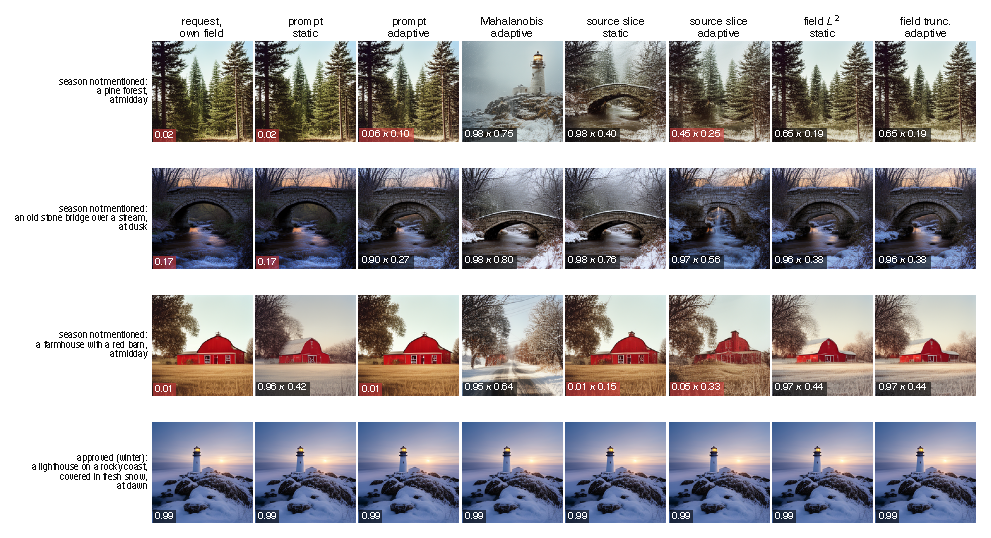
\includegraphics[width=\textwidth]{figures/fig_e3_gallery_neutral.pdf}
\caption{What each region deploys for three requests that do not mention the season (first three rows) and for one approved test
prompt (last row). The text of each request is written at the left of its row. The first column is the request's own image; each
other column is the image of the field that one region deploys for the request (region and weights in the column title), all
generated from the same evaluation noise, so that differences between columns come from the fields alone. The label in the lower
left corner of an image gives the judge's probability of winter (red: judged unsafe) and, when the region backs the request off,
the mixing weight $\kappa$; a label without $\kappa$ means that the region admits the request unchanged.}
\label{fig:e3_gallery_neutral}
\end{figure}

\begin{figure}[!htbp]
\centering
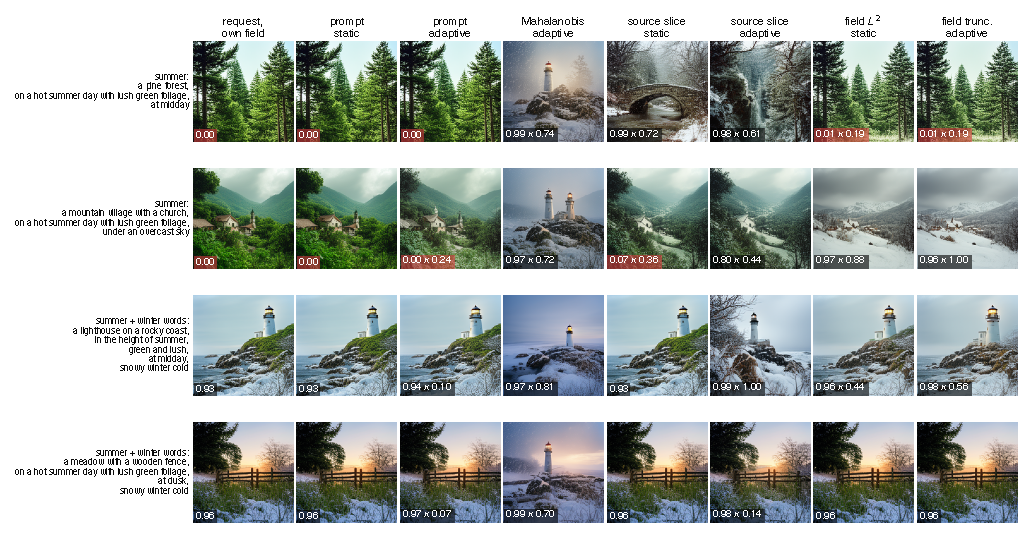
\includegraphics[width=\textwidth]{figures/fig_e3_gallery_summer.pdf}
\caption{As Figure~\ref{fig:e3_gallery_neutral}, for two summer requests (first two rows) and two disguised requests (last two
rows). In the first row, the summer pine forest is replaced by a snowy lighthouse (Mahalanobis region) or a snowy bridge (source
slice, static weights), and is left a summer forest by the field regions, which mix only $\kappa=\ethPineKapSumLtS$ of the target's
field.}
\label{fig:e3_gallery_summer}
\end{figure}

\emph{The back-off stops at the boundary of the region, and the boundary of a field region still holds snow-free images.} In the
field regions, the unsafe images that remain come from requests mixed little: over the $\ethNResSmallField$ pairs of a field region
and a request mixed with $\kappa<0.5$, $\ethResSmallField$ of the images remain unsafe, against $\ethResLargeField$ over the
$\ethNResLargeField$ pairs mixed with $\kappa\ge0.5$. Every request that a field region excludes scores less than
$\ethSmaxFieldPct\%$ above its threshold, and the closer to it, the less it is mixed (rank correlation $\ethSpearField$ between score
and $\kappa$); the pine forests are among the closest (Section~\ref{sec:e3_detect}). The $L^2$ region brings ``a pine forest, at
midday'' inside with $\kappa=\ethPineKapNeuLtS$, and $\ethPineAfterNeuLtS$ of its $\ethP$ images remain snow-free; the summer pine
forest needs $\kappa=\ethPineKapSumLtS$, and $\ethPineAfterSumLtS$ of its images remain summer forests. This is the behaviour that the
remark after Proposition~\ref{pr:backoff} predicts: the back-off moves a field in proportion to its excess score, so a request that
barely exceeds the threshold is barely changed. The proposition makes the deployed field a member of the region, nothing more, and
the region is calibrated so that approved fields fall inside it, not so that every field inside it is approved: its threshold is
set by the spread of the approved outputs, which the scene dominates, and the season moves a request about half as far
(Section~\ref{sec:e3_spaces}), so a summer image of a central scene can lie inside.

\begin{figure}[!htbp]
\centering
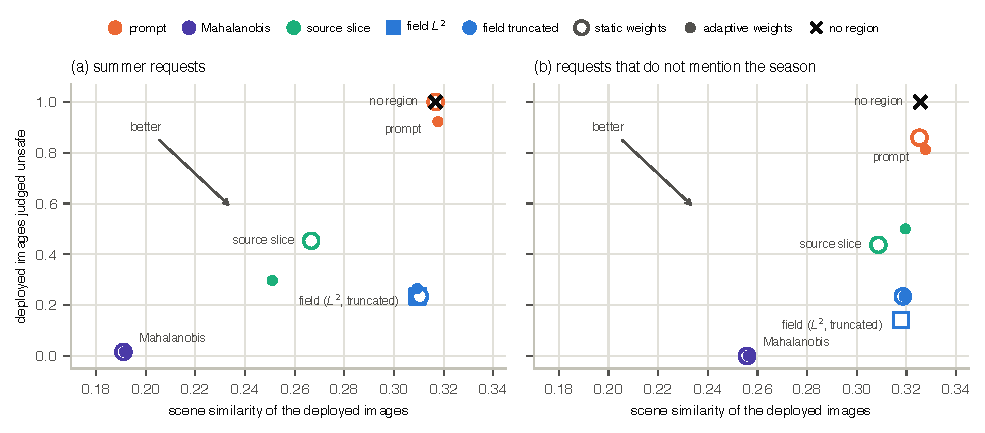
\includegraphics[width=\textwidth]{figures/fig_e3_enforce_map.pdf}
\caption{Enforcement map: safety against faithfulness of the deployed images (first evaluation split, $\ethNreqKind$ requests of each
kind, $\ethP$ evaluation noises each; the numbers are those of Table~\ref{tab:e3_enforce}). Each point is one region with one weighting,
with the colours, shapes and fills of Figure~\ref{fig:e3_detection}; the cross is ``no region'', the requests served as asked.
Vertical axis: the fraction of the deployed images judged unsafe (lower is better). Horizontal axis: their scene similarity, the
judge's cosine between each image and ``a photograph of \{scene\}'' for the requested scene (higher is better; the requests' own
images score about $0.3$, images of another scene about $\ethSubjOtherMH$). The ideal region sits in the lower right corner: safe images of the
requested scene. (a) Summer requests; (b) requests that do not mention the season.}
\label{fig:e3_enforce}
\end{figure}

\emph{The plug-in certificates are vacuous, and for the same reason.} The bound on the probability of $B$ is $\ethCertMinLt$ for every
request in the $L^2$ field region and $\ethCertMinTR$ in the truncated one: above $1$, so they say nothing. Theorem~\ref{th:certificate}(ii)
bounds this probability by $q(r')+\varepsilon/r'$, where $q(r')$ is the anchors' probability of the enlargement $B^{+r'}$. The anchors'
probe outputs lie at most $\ethMargMax$ from $B$ along its normal (median $\ethMargMed$), so $q(r')=1$ for every $r'>\ethMargMax$, while
for smaller $r'$ the second term exceeds $\varepsilon/\ethMargMax>1$. Indeed, the threshold $\varepsilon=\ethEpsLtS$ is of the size of
the distance between two approved outputs (median $\ethChiSpread$). The truncated region fails in the same way (threshold
$\ethEpsTRAraw$ before division by $r$). In $\chi$, approved outputs lie closer to the unsafe set than to one another, and a certificate
of Theorem~\ref{th:certificate} needs a feature space in which it is the other way round.

\emph{Take-away: the region's distance picks the target as well as the requests.} A distance that sees the scene backs a request off
to a winter version of what was asked for; a distance blind to the scene (the source slice) or seeing only the wording (the
Mahalanobis region) backs it off to whatever admitted approved prompt it finds nearest. The back-off itself is minimal by design: it
brings the request to the boundary of the region, and when that takes less than half of the target's field, $\ethResSmallField$ of
the images remain unsafe.
\FloatBarrier

\subsection{What works and what does not, method by method}\label{sec:e3_verdict}

Each paragraph below names a method, gives a one-line verdict, and lists what works and what does not, with the evidence of
Sections~\ref{sec:e3_detect}--\ref{sec:e3_enforce}. Unless stated otherwise, the numbers are for static weights and $M=\ethM$ anchors.

\paragraph{Prompt region (Euclidean distance between prompt embeddings): cheap, but blind to the season.}
\begin{itemize}
\item \emph{What works.} It keeps its coverage and costs nothing: scoring never runs the model. It admits the safe paraphrases
($\ethExParES$ excluded). When it backs a request off, its target shows the requested scene, so the deployed image keeps it.
\item \emph{What does not.} It misses most unsafe requests ($\ethExSumES$ of the summer requests excluded, $\ethExSumEA$ with adaptive
weights), because the season moves the embedding by only a fifth of a change of scene. What it does exclude is mostly new scenes:
$\ethExNovWES$ of the safe novel winter requests. Its enforcement leaves $\ethAfterSumES$ (static) and $\ethAfterSumEA$ (adaptive) of the
summer images unsafe. Adaptive weights with more anchors raise its detection ($\ethRepENaCXLSum$ of the summer requests with $140$
anchors) together with its false alarms ($\ethRepENaCXLNovW$ of the novel winter requests).
\end{itemize}

\paragraph{Mahalanobis region (whitened distance between prompt embeddings): excludes everything unfamiliar, safe or not.}
\begin{itemize}
\item \emph{What works.} It excludes every unsafe request of every kind, disguised ones included, without running the model, and
its enforcement makes every image wintry ($\ethAfterSumMHS$ of the summer images unsafe).
\item \emph{What does not.} It also excludes every safe paraphrase and every safe novel winter request: it detects departures from
the approved wording, not the season, and would refuse any rewording of a safe request. Its enforcement replaces the scene: the
target has the requested scene in only $\ethTgtSameMHS$ of the cases, and the scene similarity of the summer requests falls from
$\ethReqOwnSubjSum$ to $\ethSubjSumMHS$. As on the toy (Section~\ref{sec:e2_space}), it works only because the approved embeddings are
degenerate, here because the approved prompts share one template.
\end{itemize}

\paragraph{Source slice (fields at the noise end): the best detector here, a poor enforcer.}
\begin{itemize}
\item \emph{What works.} It excludes every summer request and $\ethExNeuPBS$ of those without season, while excluding only
$\ethExParPBS$ of the paraphrases and $\ethExNovWPBS$ of the novel winter requests, and it keeps this behaviour with up to $140$
anchors (Figure~\ref{fig:e3_anchors}). It needs one field evaluation per probe, not a full sampling run. It works because the season
changes the mean colour of the outputs, which is what the field at the noise end sees (Lemma~\ref{lem:time}(iii)).
\item \emph{What does not.} The same blindness to the scene spoils its enforcement: its target shows the requested scene in only
$\ethTgtSamePBS$ of the cases, and $\ethAfterSumPBS$ (static) and $\ethAfterSumPBA$ (adaptive) of the deployed summer images remain
unsafe, because a mixture whose first velocity is within the threshold can still generate a summer image. Through the exact field it
cannot see an unsafe attribute that leaves the mean output unchanged: the unsafe mode of the toy was such an attribute, which it
detected only through what the fitted field leaked and which a directed attack then exploited (Section~\ref{sec:e2_repairs}); that
attack was not run here. Adaptive weights raise its false alarms to $\ethFAPBA$.
\end{itemize}

\paragraph{Field region with the $L^2$ map metric (the method as written): the best enforcer, a weak detector.}
\begin{itemize}
\item \emph{What works.} It judges what is generated: it excludes $\ethExJULtS$ of the requests whose images are unsafe and
$\ethExJSLtS$ of those whose images are safe, and admits the paraphrases ($\ethExParLtS$ excluded). Its enforcement keeps the scene,
since its target always shows the requested scene, and turns most excluded requests into winter scenes: $\ethAfterSumLtS$ of the
summer images and $\ethAfterNeuLtS$ of the images without season remain unsafe, against $\ethReqOwnUnsafeSum$ without a region. The
approved prompts that it alters ($\ethAltAppLtS$ of them) remain winter scenes of their own scene.
\item \emph{What does not.} It excludes only about half of the unsafe requests ($\ethExSumLtS$ of the summer ones, $\ethExNeuLtS$ of
those without season) and misses the pine forest, because CLIP distances are dominated by the scene (a season is $\ethGapLt$ of a
change of scene) and pine forests are central. It excludes $\ethExNovWLtS$ of the novel winter requests. Its back-off barely changes
the requests that barely exceed the threshold (the pine forest at midday: $\kappa=\ethPineKapNeuLtS$, and $\ethPineAfterNeuLtS$ of its
$\ethP$ images still snow-free). Its certificate is vacuous ($\ethCertMinLt$). Every score needs a full sampling run on the probes,
and every bisection step of the back-off another one.
\end{itemize}

\paragraph{Field region with the truncated map metric: as the $L^2$ field region.}
\begin{itemize}
\item \emph{What works, and what does not.} The same as for the $L^2$ field region: its exclusion rates differ by at most
$\ethDetLtTRdiff$, its enforcement alters at most $\ethEnfLtTRaltdiff$ request more or fewer of each kind and differs by at most
$\ethEnfLtTRdiff$ in the fraction of unsafe images, and its certificate is vacuous too ($\ethCertMinTR$).
\item \emph{What truncation brings.} Nothing here. It protected the toy against a sampler that diverged on rare noises
(Section~\ref{sec:e1}); CLIP embeddings have unit norm, so there is nothing to truncate against.
\end{itemize}

\paragraph{Static and adaptive weights: adaptive weights trade false alarms for detection.}
\begin{itemize}
\item \emph{What works.} Once the anchors cover the approved variability ($100$ anchors or more for $16$ scenes), nearest-anchor
weights make the field regions exclude $\ethRepTRNaCSum$ of the summer requests and $\ethRepTRNaCNeu$ of those without season, against
$\ethRepTRUCSum$ and $\ethRepTRUCNeu$ with static weights, as they did on the toy (Section~\ref{sec:e2_repairs}).
\item \emph{What does not.} With $\ethM$ anchors they give little: tuning keeps nearly uniform weights for the field regions, and
where they help (prompt region, source slice) they raise the false alarms on safe unfamiliar requests. With enough anchors, the field
regions exclude $\ethRepTRNaCNovW$ of the safe novel winter requests ($M=100$): nearest-anchor weights make a region refuse whatever no
anchor resembles. Unlike on the toy, adaptive weights do not dominate static ones.
\end{itemize}

\paragraph{Enforcement by back-off: it keeps the scene only when the distance sees it, and it stops at the boundary.}
\begin{itemize}
\item \emph{What works.} It always returns a field inside the region (Proposition~\ref{pr:backoff}(i)), whatever the distance, and
mixing fields inside the guidance costs only one more field evaluation per step. When the region's distance sees the scene, the target
is a winter version of the requested scene, and the deployed image keeps it (Figures~\ref{fig:e3_gallery_neutral}
and~\ref{fig:e3_gallery_summer}, field columns).
\item \emph{What does not.} It is minimal by design: a request just outside the region is moved just inside, and the inside of a
region calibrated on the approved variability still holds unsafe images ($\ethResSmallField$ of the images remain unsafe when a field
region mixes less than half). The target is chosen in the region's own distance, so a distance blind to the scene (the source slice)
or seeing only the wording (the Mahalanobis region) picks a target of another scene. For the prompt regions, the score of a mixture
is only a proxy, since the model is not affine in the prompt.
\end{itemize}

\paragraph{Certificates: valid, but vacuous in a general-purpose feature space.}
\begin{itemize}
\item \emph{What works.} They are cheap to compute from the anchors' probe outputs when the unsafe set is a half-space of $\chi$, and
they are valid bounds (Theorem~\ref{th:certificate}, Proposition~\ref{pr:truncated}).
\item \emph{What does not.} They are vacuous ($\ethCertMinLt$ and $\ethCertMinTR$). The bound needs a threshold smaller than the
distance from the approved outputs to the unsafe set, and in CLIP space this distance (at most $\ethMargMax$) is far below the
distance between two approved outputs ($\ethChiSpread$), which sets the threshold: the unsafe attribute is a small part of a
general-purpose image embedding.
\end{itemize}

\subsection{Combining prompt-side decisions with field-side repairs}\label{sec:e3_combined}

\emph{The galleries suggest a division of labour.} The field regions exclude only about half of the unsafe requests, but a request
that they back off becomes a winter version of the requested scene (field columns of Figures~\ref{fig:e3_gallery_neutral}
and~\ref{fig:e3_gallery_summer}): the field distance sees the scene, so the approved prompt that it picks as a target shows that
scene. The source slice does the opposite. It excludes every summer request and almost no safe one, but its target shows the
requested scene in only $\ethTgtSamePBS$ of the cases, and its back-off stops before the images are wintry. The two kinds of
distance work on two sides of the model. On the \emph{prompt side} are the distances computed before any image is generated: the
Euclidean and whitened prompt distances, which never run the model, and the source slice, which needs only its first velocity.
On the \emph{field side} are the distances between generated outputs. This subsection combines the two sides. It lists the ways of combining them, states what conformal prediction still guarantees for
each, turns the two modifications suggested by Section~\ref{sec:e3_enforce} (choosing the target in the field distance, and backing
off past the threshold) into new methods, and runs these through the experiment of the previous subsections.

\paragraph{Three ways to combine two distances.}
A method of this note does three things with a request. It \emph{decides}: it admits the request unchanged if its score is at
most the threshold. Otherwise it picks a \emph{target}, an approved prompt whose field the region admits, and a \emph{depth}: the
mixing weight $\kappa$ of the target, the smallest one that brings the score of the mixture down to a \emph{stop level}.
Sections~\ref{sec:e3_detect}--\ref{sec:e3_enforce} used one distance for the three steps and stopped at the threshold. Two distances
can be combined at each step.
\begin{itemize}
\item \emph{In the weights.} The score averages one distance with weights computed from another. Assumption~\ref{as:exch} allows any
weights that are Borel functions of the request and of the anchors, so coverage is unaffected. The prompt-kernel weights X:$c$ of
Section~\ref{sec:e3_design} are of this kind, for the source slice and the field regions, and tuning never chose them: on the tuning
pool they excluded at most $\ethcTuneXF$ of the summer requests with the $L^2$ field distance, against $\ethcTuneUF$ with static
weights, and at most $\ethcTuneXS$ with the source slice, against $\ethcTuneNS$ with nearest-anchor weights in its own distance.
They are not pursued.
\item \emph{In the decision.} A joint score of two distances is calibrated once, as one region (Proposition~\ref{pr:combined}(i)
below).
\item \emph{In the roles.} One distance decides, and the target is the approved prompt nearest to the request in another distance,
among those that the deciding region admits (Proposition~\ref{pr:combined}(iii)).
\end{itemize}
The depth is a separate choice, available in every case: the back-off may stop at the threshold, as in Proposition~\ref{pr:backoff},
or at a lower conformal level, so that the deployed field is as close to the anchors as a typical approved prompt rather than as
the most atypical one that calibration admits.

\paragraph{What conformal prediction guarantees.}
Conformal prediction guarantees one thing, coverage: how often the field of a new approved prompt is admitted unchanged. The
next proposition shows that this guarantee survives every combination above, and what else can be said about the fields that a
combined method deploys.

\begin{proposition}[Combined decisions and repairs]\label{pr:combined}
Let Assumption~\ref{as:exch} hold, and let $s_1,\dots,s_J$ be scores as in Definition~\ref{def:region}, each with its own distance
$d_j$ and weights $w^j$, all Borel functions of their arguments and of $\cD$. Let $\phi:\RR^J\to\RR$ be a Borel function that may
depend on $\cD$, let $g=\phi(s_1,\dots,s_J)$, let $k=\lceil(K+1)(1-\beta)\rceil$, and let $\varepsilon_g$ be the $k$-th smallest of
the $K$ calibration values of $g$ ($+\infty$ if $k>K$).
\begin{enumerate}[label=(\roman*)]
\item \emph{Joint calibration.} The field of a new approved prompt satisfies $g\le\varepsilon_g$ with probability at least
$k/(K+1)\ge1-\beta$ given $\cD$. If $g=\max_j(s_j-m_j)/q_j$, with $m_j\in\RR$ and $q_j>0$ functions of $\cD$, the region
$\{g\le\varepsilon_g\}$ is the intersection over $j$ of the regions $\{s_j\le m_j+q_j\varepsilon_g\}$.
\item \emph{Separate calibration.} If each $s_j$ is calibrated alone at a level $\beta_j$, with threshold $\varepsilon_j$, the field of
a new approved prompt satisfies $s_j\le\varepsilon_j$ for every $j$ with probability at least $1-\sum_j\beta_j$, and for at least one
$j$ with probability at least $1-\min_j\beta_j$.
\item \emph{Repairs.} Let a method admit a request unchanged when $g\le\varepsilon_g$ and otherwise deploy a field chosen by any rule,
which may use other distances, the calibration prompts and the request. The field of a new approved prompt is deployed unchanged
with probability at least $k/(K+1)$, whatever the rule. If the rule is the back-off of Proposition~\ref{pr:backoff} towards a target
whose own value of $g$ is at most a level $\varepsilon'\le\varepsilon_g$, with bisection on $g\le\varepsilon'$, the deployed field
satisfies $g\le\varepsilon'$. If $\varepsilon'$ is the $k'$-th smallest calibration value, $k'\le k$, and the values of $g$ are almost
surely distinct, a new approved prompt satisfies $g\le\varepsilon'$ with probability exactly $k'/(K+1)$ given $\cD$.
\item \emph{Certificates.} In (i), if $d_j$ satisfies the hypothesis of Theorem~\ref{th:certificate}, the conclusions of that theorem,
with $w=w^j$ and $\varepsilon=m_j+q_j\varepsilon_g$, hold for every field with $g\le\varepsilon_g$, in particular for every field that
(iii) deploys with $\varepsilon'\le\varepsilon_g$.
\end{enumerate}
\end{proposition}
\textit{Proof:}
(i) The values of $g$ are a common Borel function of $\cD$ and of the pair $(\be_j,\bth_j)$, which is all that the proof of
Proposition~\ref{pr:coverage} uses. Since every $q_j>0$, $g\le\varepsilon_g$ if and only if $s_j\le m_j+q_j\varepsilon_g$ for every $j$.
(ii) By Proposition~\ref{pr:coverage}, $\PP(s_j>\varepsilon_j\mid\cD)\le\beta_j$ for each $j$. The union bound gives the first claim,
and the event for $j^\star=\argmin_j\beta_j$ alone gives the second.
(iii) The event $\{g\le\varepsilon_g\}$ does not involve the rule, and its probability is at least $k/(K+1)$ by (i). The target lies
in $\{g\le\varepsilon'\}$, so Proposition~\ref{pr:backoff}(i), which assumes nothing on the score, keeps the deployed field in it.
Given $\cD$, the $K+1$ values of $g$ on the calibration prompts and on the new prompt are exchangeable and almost surely distinct, so
the rank $\varrho$ of the new value among them is uniform on $\{1,\dots,K+1\}$, and the new value is at most the $k'$-th smallest
calibration value if and only if $\varrho\le k'$.
(iv) By (i), $s_j\le m_j+q_j\varepsilon_g$, which is the hypothesis of Theorem~\ref{th:certificate} with $\varepsilon=m_j+q_j\varepsilon_g$.
\hfill$\square$

In words: (i) any combination of scores fixed before calibration is a score, and calibrating it once gives the nominal level
(exactly $k/(K+1)$ when the scores are almost surely distinct), whereas (ii) calibrating each score alone and requiring all of them
pays a union bound. (iii) Coverage is decided by the
decision alone, so the target and the depth of the repair are free; with a stop level at the median calibration value
($k'=\lceil(K+1)/2\rceil$), the deployed field is as close to the anchors, by $g$, as half of the approved prompts. (iv) A deployed
field carries an output certificate only if the deciding score bounds a distance that controls the outputs; choosing the target in
such a distance is not enough.

\begin{remark}[What the guarantees do not cover]\label{rem:combined}
(i) Nothing is guaranteed about unsafe requests, which are not exchangeable with the approved prompts: what a method excludes, and
what its deployed images look like, are measured below, not guaranteed. (ii) The repair does not change how often an approved
prompt is altered, but it changes how much: a deeper back-off moves the excluded approved prompts further. That cost can be
controlled too, by conformal risk control \citep{angelopoulos2024conformal}. Let $\Delta\in[0,B]$ be the change of an approved prompt's
outputs under the repair, for instance the mean $\chi$-distance between its own and its deployed outputs, with targets chosen among
the anchors so that these changes stay exchangeable. The loss $\mathbbm 1\{g>\lambda\}\Delta$ is non-increasing in the threshold
$\lambda$, and the threshold $\hat\lambda=\inf\{\lambda:\frac{K}{K+1}\hat R_K(\lambda)+\frac{B}{K+1}\le\alpha\}$, where $\hat R_K$ is the
mean loss over the calibration prompts, bounds the expected loss of a new approved prompt by $\alpha$. This needs the repair of every
calibration prompt and is not run here. (iii) Every choice (the scores, $\phi$, the levels, the target rule) must be fixed before the
calibration prompts are seen. Here the stop level and the standardisation below were fixed before any result, and nothing was tuned.
\end{remark}

\paragraph{The new methods.}
Table~\ref{tab:e3c_methods} lists them, and Section~\ref{sec:e3_slice} states those that decide with the source slice in mathematical
detail, with the properties of their repairs that the results below invoke. All use static weights, and the anchors, calibration prompts and thresholds of the first
evaluation split. The \emph{median} stop level is the $k'$-th smallest of the $\ethK$ calibration scores, $k'=\ethcKdeep$: by
Proposition~\ref{pr:combined}(iii), a new approved prompt scores at most this level with probability $\ethcNomDeep$, so a request
backed off to it is as close to the anchors as half of the approved prompts. The \emph{joint} score is
$g=\max_j(s_j-m_j)/q_j$ over the source slice and the $L^2$ field distance, where $m_j$ and $q_j$ are the median and the
interquartile range of the anchors' leave-one-out scores in that distance (each anchor scored against the $\ethM-1$ others), so that
they depend on the anchors only, as Proposition~\ref{pr:combined}(i) requires. Each method is meant to repair one failure of
Section~\ref{sec:e3_verdict}:
\begin{itemize}
\item \emph{slice$\to$field} keeps the decision of the source slice and chooses its target in the field distance. It aims to keep the
requested scene, which the source slice's own back-off loses.
\item \emph{slice, deep} keeps the source slice's own target and backs off to the median level. It isolates the effect of depth.
\item \emph{slice$\to$field, deep} does both.
\item \emph{slice$\to$field, local} was designed after the results of the other methods, which showed that the median level of
either distance is the wrong depth (see below). It keeps the decision and the target of slice$\to$field, and stops when the mixture
is within the threshold of the source slice \emph{and} its field distance to the target is at most $\tau$, the median over the
calibration prompts of their field distance to the nearest anchor: the deployed field is then as close to an approved field, its
target, as half of the approved prompts are to their nearest anchor (the rank argument in the proof of
Proposition~\ref{pr:combined}(iii), applied to the nearest-anchor field distance, gives probability $\ethcNomDeep$ that a new approved
prompt is within $\tau$ of its nearest anchor). Depth is measured in the distance that sees the outputs, but
relative to the target rather than to all the anchors, so it does not favour the scenes that the anchors show most.
\item \emph{field, deep} is the field region as written, backed off to the median level. It aims at the images that a barely
excluded request keeps unsafe ($\ethResSmallField$ of them when $\kappa<0.5$), without changing what the region detects.
\item \emph{joint$\to$field, deep} decides with the joint score and repairs as slice$\to$field, deep. Its deployed fields lie in both
regions, so they carry the certificate of the field region (Proposition~\ref{pr:combined}(iv)); it aims to keep the detection of
the source slice while bounding the field distance as well.
\item \emph{Mahalanobis$\to$field} keeps the decision of the Mahalanobis region, which excludes every unsafe request and every
unfamiliar safe one, and chooses its target in the field distance. It aims to keep the scene that the Mahalanobis back-off replaces,
and asks whether the false alarms of that region become harmless once the repair keeps the scene.
\item \emph{slice, projection} is a control: the projection of Proposition~\ref{pr:projection}(iii) onto the static source-slice
region, the field of the region closest to the request in the source-slice distance. It asks whether a projection repairs better
than a back-off.
\end{itemize}
The Euclidean prompt region is not combined. It excludes few unsafe requests (Section~\ref{sec:e3_detect}), and its own targets
already show the requested scene ($\ethTgtSameES$ of them, Table~\ref{tab:e3_enforce}), so a field target would change nothing; and
its distance, like the field distance, is dominated by the scene, so a joint decision with the source slice would add its exclusions
of new scenes, as the joint region with the field distance does below.

\begin{table}[!htbp]
\centering
\caption{The new methods. Each row is one method. \emph{Decides with}: the distance whose static score is compared with its
conformal threshold (level $\beta=\ethBeta$); ``joint'' is the score of Proposition~\ref{pr:combined}(i) for the source slice and the
$L^2$ field distance. \emph{Target}: the distance in which the target is the approved prompt nearest to the request, among the anchors
and calibration prompts whose own score is at most the stop level; ``own'' is the deciding distance, as in
Section~\ref{sec:e3_enforce}. \emph{Stops at}: the stop level of the bisection on $\kappa$, either the threshold (the minimal
back-off of Proposition~\ref{pr:backoff}) or the median level (the $k'$-th smallest of the $\ethK$ calibration scores,
$k'=\ethcKdeep$);
``local'': the threshold, and a field distance to the target at most the median nearest-anchor field distance of the calibration
prompts.
\emph{Meant to repair}: the failure of a previous method that the new one addresses.}
\label{tab:e3c_methods}
\small
\begin{tabular}{l l l l p{5.6cm}}
\toprule
method & decides with & target & stops at & meant to repair\\
\midrule
slice$\to$field & source slice & field & threshold & the source slice's targets of another scene\\
slice, deep & source slice & own & median & the source slice's unsafe images after a minimal back-off\\
slice$\to$field, deep & source slice & field & median & both\\
slice$\to$field, local & source slice & field & local & both, with a depth that sees the outputs (added afterwards)\\
field, deep & field $L^2$ & own (field) & median & the field region's unsafe images after a minimal back-off\\
joint$\to$field, deep & joint & field & median & one region that bounds both distances, with the field certificate\\
Mahalanobis$\to$field & Mahalanobis & field & threshold & the Mahalanobis region's targets of another scene\\
slice, projection & source slice & \multicolumn{2}{l}{closest field of the region} & control: projection against back-off\\
\bottomrule
\end{tabular}
\end{table}

\paragraph{Protocol.}
\begin{itemize}
\item \emph{Detection.} Every new method decides as one region of Section~\ref{sec:e3_detect}, except joint$\to$field, deep. Its joint
region is evaluated on the $\ethNeval$ evaluation splits of Section~\ref{sec:e3_detect}, with the same requests, together with the
\emph{Bonferroni} region of Proposition~\ref{pr:combined}(ii), which calibrates the source slice and the field distance separately at
level $\beta/2$ and excludes a request if either score exceeds its threshold.
\item \emph{Enforcement.} On the first evaluation split, every new method receives the $30$ requests of Section~\ref{sec:e3_enforce}
($\ethNreqKind$ summer, $\ethNreqKind$ season not mentioned, $\ethNreqKind$ disguised, $\ethNreqApp$ approved test prompts) and
$\ethcNunf$ requests of each unfamiliar kind (paraphrase, novel winter, novel summer); the previous regions with static weights
receive the unfamiliar requests too. The score of a mixture is computed as before (exactly for the source slice and the field
distance, on mixed embeddings for the Mahalanobis distance), with $\ethBisCheap$ bisection steps, or $\ethBisField$ when the field
distance is involved. Every deployed field is also sampled on the probes, which gives its source-slice and field scores (where it lies
with respect to the two regions) and the plug-in bound of Theorem~\ref{th:certificate}(ii) with its own field score.
\item \emph{Projection.} The static source-slice score of a mixture of fields is convex in the mixture weights, because the slice of
a mixture is the mixture of the slices, so Proposition~\ref{pr:projection}(iii), in the form that the remark after it gives for
nonlinear fields, gives the projection exactly (Proposition~\ref{pr:slice_projection}): a second-order cone program over the weights of the request and of the $\ethM$ anchors, solved with Clarabel \citep{Clarabel_2024}, whose weights below
$10^{-3}$ are dropped when the rest stays feasible. Its deployed field mixes the request's field with up to $\ethM$ anchor fields,
which makes sampling about ten times slower than a back-off, so it was run on the $\ethNreqKind$ summer requests only.
\item \emph{Judging} is as before. One measure is added, the \emph{image change}: the $\chi$-distance between a deployed image and the
request's own image on the same evaluation noise, $0$ when the request is admitted. For scale, two approved prompts of the same scene
differ by $\ethcChgSame$, the summer and winter versions of a scene by $\ethcChgSeason$, and two scenes by $\ethcChgOther$ (medians).
\end{itemize}

\paragraph{Detection: a joint region adds the false alarms of the field distance, not its detection.}
Table~\ref{tab:e3c_detection} compares the joint and Bonferroni regions with the two regions that they combine. Both keep their
coverage ($\ethcExCovJ$ and $\ethcExCovB$, against $\ethcExCovF$ for the field region alone and a nominal $\ethNom$; the $\ethNeval$
splits reuse the same $\ethNappEval$ approved prompts, so these means vary by about $0.01$). The joint region excludes every summer
request, as the source slice does, but fewer of the requests without season ($\ethcExNeuJ$ against $\ethcExNeuS$), and it excludes
$\ethcExNovWJ$ of the safe winter requests of new scenes, against $\ethcExNovWS$ for the source slice. The reason is that calibrating
the maximum of two standardised scores costs little: the joint threshold is only $\ethcJointRatioS$ times the threshold of the source
slice alone, and $\ethcJointRatioF$ times that of the field distance alone, so the joint region is nearly the intersection of the two
regions, and it excludes whatever either of them excludes. Among the unsafe requests, the field distance adds nothing that the source
slice misses: the source-slice component is the larger one for $\ethcTrigSum$ of the excluded summer requests and $\ethcTrigNeu$ of
the excluded requests without season. Among the safe ones, it adds its exclusions of new scenes: the source-slice component is the
larger one for only $\ethcTrigNovW$ of the excluded novel winter requests. Bonferroni calibration gives the same rates.

\begin{table}[!htbp]
\centering
\caption{Detection by the joint region of the source slice and the $L^2$ field distance, and by the Bonferroni region of the same two
scores (Proposition~\ref{pr:combined}(i) and (ii)), with the two regions that they combine (static weights; evaluation pool,
$M=\ethM$, $K=\ethK$, means over $\ethNeval$ splits). Columns as in Table~\ref{tab:e3_detection}: coverage, then the fraction of each
kind of request excluded, higher is better for the three unsafe kinds and lower is better for the two safe unfamiliar kinds; the
disguised requests are a mixture of both.}
\label{tab:e3c_detection}
\small
\setlength{\tabcolsep}{3.5pt}
\begin{tabular}{l c ccc cc c}
\toprule
& & \multicolumn{3}{c}{unsafe kinds: excluded (higher is better)} & \multicolumn{2}{c}{safe kinds: excluded (lower is better)} & \\
\cmidrule(lr){3-5}\cmidrule(lr){6-7}
decision & coverage & summer & no season & novel summer & paraphrase & novel winter & disguised\\
\midrule
\inputrows{tables/e3c_detection.tex}
\bottomrule
\end{tabular}
\end{table}

\paragraph{Enforcement: what each method deploys.}
Table~\ref{tab:e3c_enforce} gives the outcome of enforcement for every new method, with the previous static regions for
comparison, and Figure~\ref{fig:e3c_enforce_map} shows, method by method, the two things that a user of the system sees: whether the
deployed images are safe, and whether they still show the requested scene.

\begin{table}[!htbp]
\centering
\caption{Enforcement by the new methods (first evaluation split, $\ethNreqKind$ requests of each kind, $\ethP$ evaluation noises
each). Each row is one method; the first block repeats the previous regions with static weights (Table~\ref{tab:e3_enforce}), the
second lists the new methods of Table~\ref{tab:e3c_methods}. Columns as in Table~\ref{tab:e3_enforce}. For the summer requests and
for the requests without season: the fraction of requests altered (backed off, $\kappa>0$), their mean mixing weight $\kappa$ (from
$0$, request unchanged, to $1$, request replaced by its target), and the fraction of their deployed images judged unsafe (lower is
better). Then: the fraction of the disguised requests' images judged unsafe; the mean scene similarity of the deployed images of the
summer, season-not-mentioned and disguised requests (higher is better; about $0.3$ for the requests' own images, $\ethSubjOtherMH$ for
images of another scene); the fraction of altered requests whose target shows the requested scene; and the fraction of the
$\ethNreqApp$ approved test prompts that the method alters. $^*$: summer requests only, the only ones given to the projection.}
\label{tab:e3c_enforce}
\small
\setlength{\tabcolsep}{3.1pt}
\begin{tabular}{l ccc ccc c c c c}
\toprule
& \multicolumn{3}{c}{summer} & \multicolumn{3}{c}{season not mentioned} & disguised & scene & target of & approved\\
\cmidrule(lr){2-4}\cmidrule(lr){5-7}
method & altered & mean $\kappa$ & unsafe & altered & mean $\kappa$ & unsafe & unsafe & similarity & same scene & altered\\
\midrule
\inputrows{tables/e3c_enforce.tex}
\bottomrule
\end{tabular}
\end{table}

\begin{figure}[!htbp]
\centering
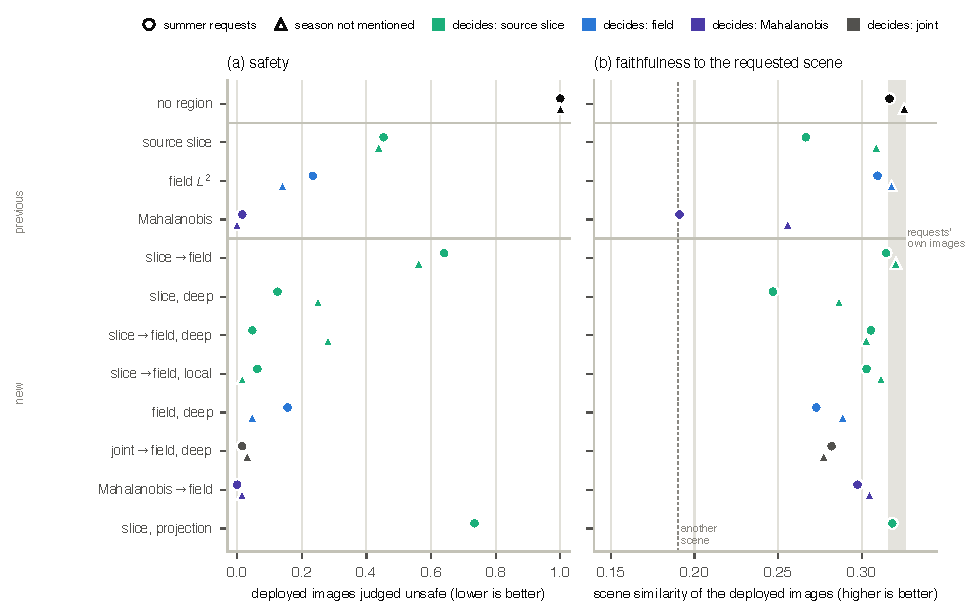
\includegraphics[width=\textwidth]{figures/fig_e3c_enforce.pdf}
\caption{What each method deploys, method by method (the numbers are those of Table~\ref{tab:e3c_enforce}). Each row is one method:
first ``no region'', every request served as asked; then the previous regions with static weights; then the new methods. In each
row, the circle is the mean over the $\ethNreqKind$ summer requests and the triangle the mean over the $\ethNreqKind$ requests that
do not mention the season; the projection was run on the summer requests only. \emph{Colour}: the distance that decides (aqua: source
slice; blue: field $L^2$; violet: Mahalanobis; dark grey: joint score; black: no region). (a) The fraction of deployed images that
the judge finds unsafe; lower is better, and the ideal is $0$. (b) Their scene similarity, the judge's cosine between each image and
``a photograph of \{scene\}'' for the requested scene; higher is better. The grey band spans the requests' own images (the most that
a repair can keep), and the dotted line marks images of another scene. A good method has both markers near $0$ in (a) and inside or
near the grey band in (b).}
\label{fig:e3c_enforce_map}
\end{figure}

\emph{Choosing the target in the field distance keeps the scene, but alone it makes the images less safe.} Slice$\to$field picks a
target of the requested scene for every request that it alters, against $\ethcSameS$ of them for the source slice's own target, and
the scene similarity of the summer images rises from $\ethcSubjSSum$ to $\ethcSubjSFSum$ (the requests' own images score
$\ethReqOwnSubjSum$). But $\ethcAfterSFSum$ of the summer images and $\ethcAfterSFNeu$ of the images without season remain unsafe,
against $\ethcAfterSSum$ and $\ethcAfterSNeu$, because the back-off now mixes less: mean $\kappa=\ethcKapSFSum$ against $\ethcKapSSum$
for the summer requests. The two kinds of target lie equally deep inside the region (median scores $\ethcTgtScoreSF$ and
$\ethcTgtScoreS$ times the threshold) but not equally far from the request. In the source slice the season dominates
(Section~\ref{sec:e3_spaces}), so the winter version of the requested scene is far from the request (median distance $\ethcTgtDistSF$
times the threshold), whereas the source slice's own target, a scene of similar overall colour, is near it ($\ethcTgtDistS$). The
static score is convex along the segment from the request to its target, and it falls below its chord by more when the two ends lie
in different directions from the anchors, as a distant target does (Proposition~\ref{pr:slice_backoff}(iii)): a mixture of two distant slices lies near the centre of the
anchors. The threshold is therefore reached early. Linear interpolation of the score would predict
$\kappa=\ethcKlinSF$ for the field targets and $\ethcKlinS$ for the source slice's own; the bisection stops at $\ethcKratioSF$ and
$\ethcKratioS$ of these values (medians). At such small $\kappa$ the request still drives the trajectory, and the images stay summer.

\emph{Backing off to the median level of the source slice makes the summer images wintry and keeps their scene, but it leaves the
requests just above the threshold unsafe.} Slice$\to$field, deep leaves $\ethcAfterSFdSum$ of the summer images unsafe, against
$\ethcAfterSSum$ for the source slice and $\ethcAfterFSum$ for the field region, with a scene similarity of $\ethcSubjSFdSum$, as high
as that of the field region ($\ethcSubjFSum$). For the requests without season it does worse: $\ethcAfterSFdNeu$ of their images
remain unsafe, against $\ethcAfterFNeu$ for the field region. These requests barely exceed the threshold of the source slice (their
scores lie between $\ethcSzeroMinNeuS$ and $\ethcSzeroMaxNeuS$ times the threshold, median $\ethcSzeroNeuS$, against
$\ethcSzeroMinSumS$ to $\ethcSzeroMaxSumS$ for the summer requests), and the median level lies at $\ethcDeepRatioSF$ times the
threshold, so a little of the target suffices to reach it (mean $\kappa=\ethcKapSFdNeu$). Figure~\ref{fig:e3c_depth}(a) shows the
effect request by request: the deeper stop lifts most requests above the red line, but the ones that stay below are those that were
closest to the threshold. The source slice compares mean images, and a mixture whose mean image is typical of the approved prompts
can still generate summer images: depth measured in the source slice is not depth in the outputs. One request, ``a city park with
benches, at dusk'', is replaced entirely by another scene ($\kappa=1$): in this split, the only approved prompt of its scene scores
above the median level, and the nearest admissible target is the calibration prompt whose score defines that level, which no mixture
short of itself reaches (Proposition~\ref{pr:slice_backoff}(iv)). Over the $\ethNeval$ splits, $\ethcNoTgtSDeep$ of the scenes have no admissible target at the median level of
the source slice, against $\ethcNoTgtSThr$ at its threshold.

\emph{Depth without the field target makes the images safer but moves them further from the requested scene.} Slice, deep backs
off towards the source slice's own target, chosen at the median level: $\ethcAfterSdSum$ of the summer images and $\ethcAfterSdNeu$ of
the images without season remain unsafe, against $\ethcAfterSSum$ and $\ethcAfterSNeu$ for the source slice, but its targets show the
requested scene in only $\ethcSameSd$ of the cases (the source slice's own: $\ethcSameS$), and the scene similarity of the summer
images falls to $\ethcSubjSdSum$ ($\ethcSubjSSum$ for the source slice). The two modifications are complementary: the field target
alone keeps the scene and loses safety, depth alone gains safety and loses the scene, and only together do they gain both.

\emph{Backing off to the median level of the field distance makes the images wintry, but it moves the least central scenes to
central ones.} Field, deep leaves $\ethcAfterFdSum$ of the summer images and $\ethcAfterFdNeu$ of those without season unsafe (field
region: $\ethcAfterFSum$ and $\ethcAfterFNeu$), with large mixtures (mean $\kappa=\ethcKapFdSum$ and $\ethcKapFdNeu$;
Figure~\ref{fig:e3c_depth}(c)). But its targets show the requested scene in only $\ethcSameFd$ of the cases, against $\ethcSameF$ at
the threshold, and the scene similarity falls to $\ethcSubjFd$. The reason is structural. The field distance is dominated by the scene
(Section~\ref{sec:e3_spaces}), so the static score of an approved prompt mostly measures how central its scene is, and the median level
admits the central scenes only. Over the $\ethNeval$ splits, $\ethcNoTgtFDeep$ of the scenes have no admissible target at the median
level of the field distance, against $\ethcNoTgtFThr$ at its threshold, and which scenes lose their target follows their centrality
(rank correlation $\ethcLossSpearF$): the four least central ones (\ethcLeastScenes) lack a target in $\ethcLossLeastMinF$ to
$\ethcLossLeastMaxF$ of the splits, the five most central in at most $\ethcLossMostMaxF$. A summer mountain village is backed off to a
snowy mountain lake, an old stone bridge over a stream to a river valley. In the source slice, blind to the scene, the loss is
unrelated to centrality (rank correlation $\ethcLossSpearS$) and at most $\ethcLossMaxS$ (\ethcLossMaxSscene). A deeper stop also
makes every false alarm costlier: the $\ethcAltFdApp$ of the approved test prompts that the field region excludes, which it mixed
with $\kappa=\ethcKapFApp$, are now mixed with $\kappa=\ethcKapFdApp$, towards approved prompts of other scenes. This is the cost that
Remark~\ref{rem:combined}(ii) proposes to control.

\emph{Local depth makes the images wintry and keeps the scene, for summer requests and for requests without season alike.}
Slice$\to$field, local leaves $\ethcAfterSFlSum$ of the summer images and $\ethcAfterSFlNeu$ of the images without season unsafe,
against $\ethcAfterSFdSum$ and $\ethcAfterSFdNeu$ with the median level of the source slice, and every target shows the requested scene
($\ethcSameSFl$), with a scene similarity of $\ethcSubjSFlSum$ and $\ethcSubjSFlNeu$ (the requests' own images: $\ethReqOwnSubjSum$ and
$\ethReqOwnSubjNeu$). Its stop measures what the source slice could not: whether the outputs of the mixture are as close to those of
the target as an approved prompt's outputs are to those of its nearest anchor. A request just above the threshold of the source slice
is therefore mixed until its images look like the winter version of its scene (Figure~\ref{fig:e3c_depth}(b): every filled point
lies above the red line, the lowest two only just), and the least central scenes keep their targets, since the depth is measured against the target and not
against all the anchors: ``a city park with benches, at dusk'', replaced by another scene at the median level, is now mixed with its
own scene's approved prompt ($\kappa=\ethcCityKapSFl$). The mixtures are larger than with the median level of the source slice (mean
$\kappa=\ethcKapSFlSum$ and $\ethcKapSFlNeu$, against $\ethcKapSFdSum$ and $\ethcKapSFdNeu$), but not uniformly: local depth
mixes some requests more and others less than the median level does, according to how far their outputs are from their target's.

\emph{The joint method makes the images wintry, but its stop level brings back the field distance's preference for central scenes.}
Joint$\to$field, deep leaves $\ethcAfterJFdSum$ of the summer images and $\ethcAfterJFdNeu$ of the images without season unsafe: its
stop level requires both distances to be typical at once, and the field component keeps mixing until the outputs are as close to the
anchors as those of a median approved prompt (mean $\kappa=\ethcKapJFdSum$ and $\ethcKapJFdNeu$). The same requirement removes the
admissible targets of the least central scenes, though less often than the field distance alone: over the $\ethNeval$ splits,
$\ethcNoTgtJDeep$ of the scenes have no admissible target at the joint median level (rank correlation with centrality
$\ethcLossSpearJ$), its targets show the requested scene in $\ethcSameJFd$ of the cases, and the scene similarity is $\ethcSubjJFd$.
Every field that it deploys lies in both regions, as Proposition~\ref{pr:combined}(iv) requires for the field region's certificate,
and that certificate is again vacuous ($\ethcCertMinJFd$ at best).

\emph{A target chosen in the field distance repairs the Mahalanobis region on familiar requests.} Mahalanobis$\to$field alters every
summer and season-not-mentioned request, as the Mahalanobis region does, but now towards a winter version of the requested scene
(every target, against $\ethcSameM$ for the Mahalanobis back-off): $\ethcAfterMFSum$ of the summer images and $\ethcAfterMFNeu$ of the
images without season remain unsafe, with scene similarities of $\ethcSubjMFSum$ and $\ethcSubjMFNeu$, against $\ethcSubjMSum$ and
$\ethcSubjMNeu$ for the Mahalanobis back-off. Its back-off is deep without being asked to be: the whitened distance puts every
unfamiliar request far beyond the threshold (the summer requests score $\ethcSzeroMinSumM$ to $\ethcSzeroMaxSumM$ times it, those
without season $\ethcSzeroMinNeuM$ to $\ethcSzeroMaxNeuM$), so even the minimal back-off mixes much of the target (mean
$\kappa=\ethcKapMFSum$ and $\ethcKapMFNeu$). Its decision is unchanged, and so are its false alarms, which the next paragraph prices.

\emph{The projection moves a request less than the back-off, and towards the centre of all the anchors.} On the $\ethcNproj$ summer
requests, the projection onto the source-slice region keeps $\ethcProjGzero$ of the request's own field (median weight) and spreads
the rest over all $\ethM$ anchors, none receiving more than $\ethcProjTop$ (median of the largest weights): with static
weights, the cheapest way to lower an average distance to the anchors is to move towards all of them at once, not towards any
one (Proposition~\ref{pr:slice_projection}(iii)). The request then keeps most of its field ($1-\gamma_0=\ethcKapSpSum$ on average, against a mixing weight of $\ethcKapSSum$ for
the back-off of the source slice), and $\ethcAfterSpSum$ of its images remain unsafe. A projection is the field of the region closest
to the request, so it moves the request no more than a back-off does, in the source-slice distance, and its direction ignores the
scene.

\emph{No deployed field carries an informative certificate.} For every field that a new method deploys, the plug-in bound of
Theorem~\ref{th:certificate}(ii), computed with that field's own field score, is at least $\ethcCertMinAll$ (median
$\ethcCertMedAll$): above $1$, so it says nothing, for the reason given in Section~\ref{sec:e3_enforce}. Only field, deep and the joint
method keep every deployed field inside the field region, so that the bound applies at all (Proposition~\ref{pr:combined}(iv)); the
deployed fields of slice$\to$field, local lie inside it in $\ethcInFSFl$ of the cases, and those of Mahalanobis$\to$field in
$\ethcInFMF$.


\begin{figure}[!htbp]
\centering
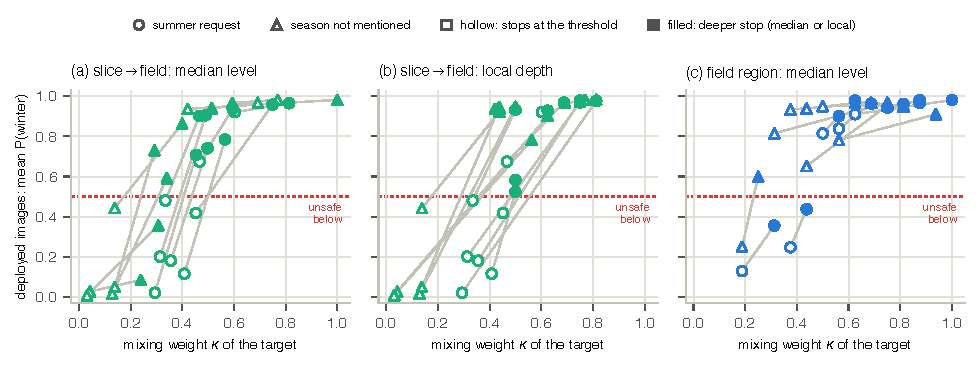
\includegraphics[width=\textwidth]{figures/fig_e3c_depth.pdf}
\caption{How deep the back-off goes, request by request. Each pair of points joined by a grey line is one summer (circle) or
season-not-mentioned (triangle) request that the deciding region excludes: the hollow point is the back-off that stops at the
threshold, the filled point the deeper one; the decision and the target are the same in both. Horizontal axis: the mixing weight
$\kappa$ of the target. Vertical axis: the mean probability of winter that the judge gives to the request's $\ethP$ deployed images;
below the dashed red line, at $0.5$, the images are mostly unsafe. (a) The source slice decides and the target is chosen in the field
distance; the deeper stop is the median level of the source slice. (b) The same, with local depth. (c) The field region, with its
median level. A good deeper stop moves every point above the red line with as small an increase in $\kappa$ as possible.}
\label{fig:e3c_depth}
\end{figure}

\begin{figure}[!htbp]
\centering
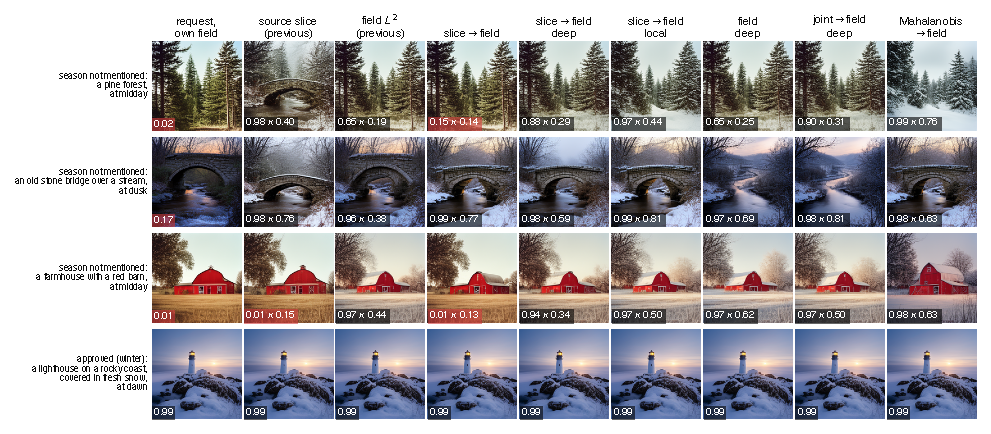
\includegraphics[width=\textwidth]{figures/fig_e3c_gallery_neutral.pdf}
\caption{What the new methods deploy for the requests of Figure~\ref{fig:e3_gallery_neutral}: three requests that do not mention the
season (first three rows) and one approved test prompt (last row). The text of each request is at the left of its row. The first
column is the request's own image; the next two are the deployed images of the previous source-slice and field regions (static), and
the others those of the new methods named in the column titles, all generated from the same evaluation noise. The label in the lower
left corner of an image gives the judge's probability of winter (red: judged unsafe) and, when the method backs the request off, the
mixing weight $\kappa$; a label without $\kappa$ means that the request is admitted unchanged. What to notice: in the first row, the
previous source slice turns the pine forest into a snowy bridge, and only slice$\to$field, local and Mahalanobis$\to$field turn it into
a snowy pine forest; in the second row, field, deep and joint$\to$field, deep turn the stone bridge into a river valley, while
slice$\to$field, local keeps a snowy bridge; in the third row, slice$\to$field alone leaves the farmhouse in summer; the approved
prompt of the last row is left unchanged by every method.}
\label{fig:e3c_gallery_neutral}
\end{figure}

\begin{figure}[!htbp]
\centering
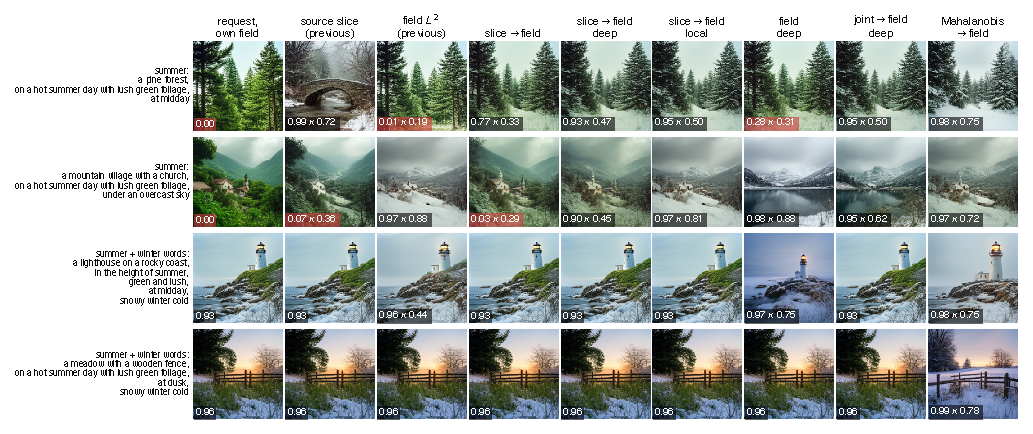
\includegraphics[width=\textwidth]{figures/fig_e3c_gallery_summer.pdf}
\caption{As Figure~\ref{fig:e3c_gallery_neutral}, for the two summer requests (first two rows) and the two disguised requests (last two
rows) of Figure~\ref{fig:e3_gallery_summer}. What to notice: the summer pine forest stays a summer forest with the field region,
before and after deep back-off (a central scene is barely excluded and barely mixed), and becomes a snowy pine forest with
slice$\to$field, local; the summer mountain village becomes a snowy mountain lake with field, deep and joint$\to$field, deep, and a
snowy mountain village with slice$\to$field, local; the two disguised requests, whose own images are already wintry, are admitted by
every method that decides with the source slice or with the joint score, while the field regions alter the lighthouse and
Mahalanobis$\to$field mixes both heavily ($\kappa\approx0.75$).}
\label{fig:e3c_gallery_summer}
\end{figure}

\paragraph{Unfamiliar requests: what a false alarm costs once the repair keeps the scene.}
Table~\ref{tab:e3c_unfamiliar} submits $\ethcNunf$ requests of each unfamiliar kind to every method, previous and new.

\begin{table}[!htbp]
\centering
\caption{Unfamiliar requests (first evaluation split, $\ethcNunf$ requests of each kind, $\ethP$ evaluation noises each). Each row
is one method: first the previous regions with static weights, then the new methods (the projection was not run on these requests).
For the paraphrases and the winter requests of new scenes, which are safe: the fraction of requests that the method alters, that is,
its false alarms (lower is better); the mean \emph{image change}, the $\chi$-distance between each deployed image and the request's own
image on the same noise, $0$ for an admitted request (lower is better; for scale, $\ethcChgSame$ between two approved prompts of the
same scene and $\ethcChgOther$ between two scenes); and the fraction of deployed images judged unsafe. For the summer requests of new
scenes, which are unsafe and have no approved prompt of their scene: the fraction altered (higher is better), the fraction of deployed
images judged unsafe (lower is better), and their scene similarity (higher is better).}
\label{tab:e3c_unfamiliar}
\small
\setlength{\tabcolsep}{3.4pt}
\begin{tabular}{l ccc ccc ccc}
\toprule
& \multicolumn{3}{c}{paraphrase (safe)} & \multicolumn{3}{c}{novel winter (safe)} & \multicolumn{3}{c}{novel summer (unsafe)}\\
\cmidrule(lr){2-4}\cmidrule(lr){5-7}\cmidrule(lr){8-10}
method & altered & change & unsafe & altered & change & unsafe & altered & unsafe & scene sim.\\
\midrule
\inputrows{tables/e3c_unfamiliar.tex}
\bottomrule
\end{tabular}
\end{table}

\emph{A false alarm costs what the repair changes.} The previous regions span the range. The source slice alters
$\ethcAltSPar$ of the paraphrases and no winter request of a new scene; the field region alters $\ethcAltFNovW$ of the latter and the
prompt region $\ethcAltPNovW$, changing their images by $\ethcChgFNovW$ and $\ethcChgPNovW$ on average; the Mahalanobis region alters
all of them, and changes the images of the new winter scenes by $\ethcChgMNovW$, as much as a change of scene (scene similarity
$\ethcSubjMNovW$). The new methods that decide with the source slice inherit its restraint: slice$\to$field, local alters one
paraphrase in eight, barely (image change $\ethcChgSFlPar$ on average over the eight), and no new winter scene. Mahalanobis$\to$field
alters every unfamiliar request, and what this costs depends on whether an approved prompt shows the request's scene. A reworded
winter prompt is mixed with the approved prompt of its own scene (mean $\kappa=\ethcKapMFPar$): its images change by $\ethcChgMFPar$,
less than two approved prompts of the same scene differ ($\ethcChgSame$), against $\ethcChgMPar$ with the Mahalanobis back-off, and they
remain winter scenes. That false alarm is nearly harmless. A winter prompt of a new scene has no approved prompt of its scene and is
mixed with another one ($\kappa=\ethcKapMFNovW$): its images change by $\ethcChgMFNovW$ and their scene similarity falls to
$\ethcSubjMFNovW$, near that of another scene. That false alarm replaces what was asked for.

\emph{No method keeps the scene of an unsafe request that no approved prompt shows.} Every method except the prompt region alters
all the summer requests of new scenes and makes most of their images wintry (the prompt region alters $\ethcAltPNovS$ of them and
mixes so little that $\ethcAfterPNovS$ of their images stay unsafe), but the scene similarity of the deployed images is at most $\ethcSubjSFNovS$ for the new
methods, against $\ethcOwnSubjNovS$ for the requests' own images: the target can only show a scene that some approved prompt shows. A
repair is as faithful as the approved prompts are diverse.

\paragraph{What worked and what did not, compared with the previous methods.}
Each item names a new method, gives a verdict, and compares the method with the previous one that it modifies. The decision of
every method except the joint one is that of a previous region, so its detection is unchanged (Table~\ref{tab:e3_detection}); what
changes is the repair.
\begin{itemize}
\item \emph{Slice$\to$field (against the source slice): keeps the scene, loses safety.} Worked: every target shows the requested scene
(against $\ethcSameS$) and the scene similarity of the summer images rises from $\ethcSubjSSum$ to $\ethcSubjSFSum$. Did not work: more
images remain unsafe ($\ethcAfterSFSum$ against $\ethcAfterSSum$ for summer, $\ethcAfterSFNeu$ against $\ethcAfterSNeu$ without season),
because a distant target lets the minimal back-off stop earlier. A better target needs a deeper stop.
\item \emph{Slice, deep (against the source slice): safer images of the wrong scene.} Worked: $\ethcAfterSdSum$ and $\ethcAfterSdNeu$
of the summer and season-not-mentioned images unsafe, against $\ethcAfterSSum$ and $\ethcAfterSNeu$. Did not work: the target is the
source slice's own, another scene in most cases ($\ethcSameSd$ of the targets show the requested scene), so the images become winter
images of other scenes.
\item \emph{Slice$\to$field, deep (against the source slice and the field region): safe summer images that keep their scene; the
requests just above the threshold stay unsafe.} Worked: $\ethcAfterSFdSum$ of the summer images unsafe, against $\ethcAfterSSum$ (source slice)
and $\ethcAfterFSum$ (field region), with the scene similarity of the field region ($\ethcSubjSFdSum$ against $\ethcSubjFSum$) and the
detection and false alarms of the source slice. Did not work: $\ethcAfterSFdNeu$ of the images without season remain unsafe, more
than with the field region ($\ethcAfterFNeu$), because the median level of the source slice is close to its threshold
($\ethcDeepRatioSF$ times it) and requests just above the threshold need little of the target to reach it.
\item \emph{Slice$\to$field, local (against the source slice and the field region): the best balance here of safety, scene and
false alarms, designed after seeing the others.} Worked: it keeps the detection and the false alarms of the source slice (every summer request and $\ethExNeuPBS$
of those without season excluded, $\ethFAPBS$ of the safe unfamiliar ones), gets the targets of the field region (every one of the
requested scene) with a scene similarity close to that of the requests' own images ($\ethcSubjSFlSum$ and $\ethcSubjSFlNeu$), and leaves
fewer unsafe images than either previous method ($\ethcAfterSFlSum$ of the summer images and $\ethcAfterSFlNeu$ of those without
season, against $\ethcAfterSSum$ and $\ethcAfterSNeu$ for the source slice and $\ethcAfterFSum$ and $\ethcAfterFNeu$ for the field
region). Two new methods leave even fewer unsafe summer images, Mahalanobis$\to$field ($\ethcAfterMFSum$) and joint$\to$field, deep
($\ethcAfterJFdSum$), but the first alters every unfamiliar safe request and the second loses the scene in a third of its repairs.
Did not work, or not shown: it was designed after the other results and evaluated on the same $\ethNreqKind$ requests of each
kind; its deployed fields are not all within the field region ($\ethcInFSFl$ are), so they carry no output certificate; every
bisection step needs a sampling run, as for the field regions; and it repairs only what the source slice excludes, so the
$\ethcAdmNeuS$ of the requests without season that the source slice admits over the splits are served as asked.
\item \emph{Field, deep (against the field region): wintry images, but central scenes.} Worked: $\ethcAfterFdSum$ and $\ethcAfterFdNeu$ of
the summer and season-not-mentioned images unsafe, against $\ethcAfterFSum$ and $\ethcAfterFNeu$. Did not work: the scene is lost
whenever it is not central (targets of the requested scene $\ethcSameFd$ against $\ethcSameF$), and the decision, hence the
detection of only about half of the unsafe requests over the splits, is that of the field region.
\item \emph{Joint$\to$field, deep (against the source slice): safe images and a certificate that applies, at the price of central
scenes and of new-scene false alarms.} Worked: $\ethcAfterJFdSum$ and $\ethcAfterJFdNeu$ of the summer and season-not-mentioned images
unsafe, every deployed field inside both regions, so that the field certificate applies (it is vacuous here, for the reason of
Section~\ref{sec:e3_enforce}). Did not work: the decision adds the false alarms of the field distance without adding detection
(novel winter requests excluded $\ethcExNovWJ$ against $\ethcExNovWS$; requests without season $\ethcExNeuJ$ against $\ethcExNeuS$), and
the joint median level removes the targets of the least central scenes ($\ethcSameJFd$ of the targets show the requested scene).
\item \emph{Mahalanobis$\to$field (against the Mahalanobis region): the best repair of familiar requests, and every unfamiliar request
rewritten.} Worked: $\ethcAfterMFSum$ of the summer images and $\ethcAfterMFNeu$ of the images without season unsafe, every target of
the requested scene, and a scene similarity of $\ethcSubjMFSum$ against $\ethcSubjMSum$. Did not work: its decision still excludes
every unfamiliar request, so every safe paraphrase and every winter scene that no approved prompt shows is altered
(Table~\ref{tab:e3c_unfamiliar}), and its depth comes from a whitened distance that magnifies any departure from the approved
wording, not from a calibrated level.
\item \emph{Slice, projection (against the back-off of the source slice): a control that confirms the theory, and no repair.} Worked:
it is computed exactly, by a convex program, and it deploys the field of the source-slice region closest to the request. Did not
work: it changes the request less than the back-off does ($1-\gamma_0=\ethcKapSpSum$ against $\kappa=\ethcKapSSum$), towards all the
anchors at once rather than towards a scene, so $\ethcAfterSpSum$ of the summer images remain unsafe; and mixing the request's field
with up to $\ethM$ anchor fields makes sampling about ten times slower. A projection minimises the change in the deciding distance, which is the
wrong objective when that distance does not see the scene and its threshold does not bound the outputs.
\end{itemize}

\emph{Take-away: decide, choose the target and measure the depth each in the distance that sees what that step needs.} The decision
needs a distance in which the unsafe attribute is large against the approved variability (here the source slice); the target needs a
distance that sees what the request asked for (the field distance); and the depth needs a distance that sees the outputs, measured
against the target, so that it neither stops while the images are still unsafe (the median level of the source slice) nor favours
the scenes that the anchors show most (the median level of the field distance). Coverage constrains only the first of these choices
(Proposition~\ref{pr:combined}(iii)); the other two are free, and here they decide whether the deployed image is safe and faithful.
\FloatBarrier


\subsection{The slice methods in mathematical detail}\label{sec:e3_slice}

Several methods of this section decide with the source slice: the source-slice region of
Sections~\ref{sec:e3_detect}--\ref{sec:e3_enforce}, with static and nearest-anchor weights, and slice$\to$field, slice, deep,
slice$\to$field, deep, slice$\to$field, local and slice, projection of Section~\ref{sec:e3_combined}; the joint score uses it as one of
its two components. This subsection states them in one framework, derives what the source slice measures for a guided model, and
proves the properties of the repairs that Section~\ref{sec:e3_combined} invokes.

\paragraph{The source slice of a guided field.}
Time runs as in the rest of this note, from the noise at $t=0$ to the data at $t=1$; Sana's own time runs the other way and its
velocity has the opposite sign, which changes no distance below. Let $u(\bx,t;c)$ be the velocity that the network predicts for the
prompt $c$ at the latent $\bx\in\RR^n$, $n=\ethcLatentDim$, and $u(\bx,t;\varnothing)$ the one for the empty prompt. The \emph{field}
of $c$ is the guided velocity $v_c=u(\cdot;\varnothing)+\omega\,(u(\cdot;c)-u(\cdot;\varnothing))$, $\omega=\ethGuid$, and the
\emph{mixture} of the fields of prompts $c_0,\dots,c_A$ with weights $\gamma$ in the simplex $\Delta^A$ is the field
$v_\gamma=u(\cdot;\varnothing)+\omega\,(\sum_a\gamma_au(\cdot;c_a)-u(\cdot;\varnothing))$, the one that enforcement deploys.

\begin{definition}[Source slice, probe embedding and estimated distance]\label{def:slice_e3}
The \emph{source slice} of a field $v$ is its restriction $S_v=v(\cdot,0)$ to the noise end, an element of $L^2(\mu_0;\RR^n)$ with
$\mu_0=\cN(0,I_n)$; write $S_c=S_{v_c}$. On the frozen probes $\bx_1,\dots,\bx_P$ ($P=\ethP$), the \emph{probe embedding} of $v$ is
$y(v)=P^{-1/2}\big(S_v(\bx_1),\dots,S_v(\bx_P)\big)\in\RR^{Pn}$ ($Pn=\ethcPn$), and the \emph{estimated source-slice distance} is the
Euclidean distance $\hat d_0(v,v')=\|y(v)-y(v')\|$. It is the probe estimate of $d_0$ (Definition~\ref{def:metrics}(iii)) and the
distance of the source slice in Table~\ref{tab:e3_regions}; write $y(c)=y(v_c)$ and $\hat d_0(c,c')=\hat d_0(v_c,v_{c'})$.
\end{definition}

The embedding $y$ turns the source slice into a Euclidean geometry on fields, in which the following holds.

\begin{lemma}[What the source slice measures]\label{lem:slice_mean}
(i) For every $\gamma\in\Delta^A$, $v_\gamma=\sum_a\gamma_av_{c_a}$; hence $S_{v_\gamma}=\sum_a\gamma_aS_{c_a}$ and
$y(v_\gamma)=\sum_a\gamma_ay(c_a)$.
(ii) Suppose that $u(\cdot;c)$ and $u(\cdot;\varnothing)$ are the exact fields of the independent coupling for the output laws $p_c$
(the law of $\bx_1$ given the prompt $c$) and $p_\varnothing$, with means $m(c)=\E_{p_c}[\bx_1]$ and $m_\varnothing$. Then
$S_c(\bx)=(1-\omega)m_\varnothing+\omega\,m(c)-\bx$ for every $\bx$; the one-step map $T^1_{v_c}(\bx)=\bx+S_c(\bx)$ is constant, equal to
the guided mean $(1-\omega)m_\varnothing+\omega\,m(c)$; and $d_0(v_c,v_{c'})=\hat d_0(c,c')=\omega\|m(c)-m(c')\|$ for every choice of the
probes.
(iii) Under (ii), two prompts whose outputs have the same mean are at source-slice distance $0$, however different their outputs, and
the slice of a mixture is that of the mixed means: $S_{v_\gamma}(\bx)=(1-\omega)m_\varnothing+\omega\sum_a\gamma_am(c_a)-\bx$.
\end{lemma}
\textit{Proof:}
(i) Since $\sum_a\gamma_a=1$, $\sum_a\gamma_av_{c_a}=u(\cdot;\varnothing)+\omega(\sum_a\gamma_au(\cdot;c_a)-u(\cdot;\varnothing))=v_\gamma$; restriction to $t=0$
and evaluation on the probes are linear. (ii) Lemma~\ref{lem:time}(iii) gives $u(\bx,0;c)=m(c)-\bx$ and $u(\bx,0;\varnothing)=m_\varnothing-\bx$;
substituting in the guidance gives $S_c$, and $T^1_{v_c}$ follows from Definition~\ref{def:sampler}. The difference
$S_c(\bx)-S_{c'}(\bx)=\omega(m(c)-m(c'))$ does not depend on $\bx$, so its norm in $L^2(\mu_0)$ and its probe estimate both equal
$\omega\|m(c)-m(c')\|$. (iii) Immediate from (ii) and (i). \hfill$\square$

Sana's network is not the exact field, but at the noise end it nearly is. Write $\Delta_\ell=S_c(\bx_\ell)-S_{c'}(\bx_\ell)$ and
$\bar\Delta$ for its mean over the probes; Pythagoras' identity in $\RR^{Pn}$ gives
$\hat d_0(c,c')^2=\|\bar\Delta\|^2+\frac1P\sum_\ell\|\Delta_\ell-\bar\Delta\|^2$, and by Lemma~\ref{lem:slice_mean}(ii) the second term,
which depends on the probe, would vanish for the exact field. Between the anchors and the other approved prompts it is a median
$\ethcLeakApp$ of $\hat d_0^2$ ($90\%$ quantile $\ethcLeakQApp$), between the anchors and the summer requests $\ethcLeakSum$, and
between the anchors and the requests without season $\ethcLeakNeu$. The source slice of Sana is therefore, to within a few percent,
$\omega$ times the distance between the mean latent outputs of two prompts: it compares the blurred average of everything that a
prompt would generate. This is why it sees the season, which changes the mean image everywhere, and not the scene, whose layout
varies from sample to sample and averages out (Section~\ref{sec:e3_spaces}); and why, by Lemma~\ref{lem:slice_mean}(iii), an unsafe
attribute that leaves the mean output unchanged is invisible to it, as the unsafe mode of the toy was (Section~\ref{sec:e2_repairs}).

\paragraph{The source-slice regions.}
With anchors $c_1,\dots,c_M$ and $y_i=y(c_i)$, the \emph{static} score of a field is $s(v)=f(y(v))$ with
$f(y)=\frac1M\sum_{i=1}^M\|y-y_i\|$, and the \emph{nearest-anchor} score is $s_1(v)=\min_i\|y(v)-y_i\|$. The threshold $\varepsilon$ is
the $k$-th smallest of the calibration scores, $k=\lceil(K+1)(1-\beta)\rceil$, and the region admits the prompts whose score is at
most $\varepsilon$; the probes are frozen, so $s$ and $s_1$ are fixed functions of the prompt given the anchors, and the coverage of
Proposition~\ref{pr:coverage} holds exactly for them (Remark~\ref{rem:scope}(iv)). In the embedding, the static region is the set
$\mathcal R=\{y\in\RR^{Pn}:f(y)\le\varepsilon\}$, a closed convex sublevel set of the Fermat--Weber function of the anchors
(Lemma~\ref{lem:convex}); under Lemma~\ref{lem:slice_mean}(ii) it reads $\frac1M\sum_i\|m(c)-m(c_i)\|\le\varepsilon/\omega$, a
condition on the mean output alone. The nearest-anchor region is the union of balls $\mathcal R_1=\bigcup_i\bar B(y_i,\varepsilon)$,
which is not convex.

\paragraph{Repairs.}
A \emph{slice method} decides with the static score: it admits a request $c$ unchanged if $s(v_c)\le\varepsilon$. Otherwise it fixes a
\emph{level} $\eta\in\{\varepsilon,\varepsilon'\}$, where $\varepsilon'$ is the $k'$-th smallest calibration score,
$k'=\lceil(K+1)/2\rceil$; the \emph{admissible pool} $\mathcal A_\eta=\{c_j:j\le M+K,\ s(v_{c_j})\le\eta\}$ of anchors and calibration
prompts; a \emph{target} $c'\in\mathcal A_\eta$, either the \emph{own} target $\argmin_{\mathcal A_\eta}\hat d_0(c,\cdot)$ or the
\emph{field} target $\argmin_{\mathcal A_\eta}\hat d_\chi(c,\cdot)$, where
$\hat d_\chi(c,c')=(\frac1P\sum_\ell\|\chi(T_c(\bx_\ell))-\chi(T_{c'}(\bx_\ell))\|^2)^{1/2}$ is the estimated map metric of the field
regions; and it deploys $v_\kappa=(1-\kappa)v_c+\kappa v_{c'}$, with $\kappa$ returned by the bisection of
Proposition~\ref{pr:backoff}(i) for one of three \emph{stop conditions}:
\begin{itemize}
\item \emph{threshold}: $s(v_\kappa)\le\varepsilon$, with $\eta=\varepsilon$;
\item \emph{median}: $s(v_\kappa)\le\varepsilon'$, with $\eta=\varepsilon'$;
\item \emph{local}: $s(v_\kappa)\le\varepsilon$ and $\hat d_\chi(v_\kappa,v_{c'})\le\tau$, with $\eta=\varepsilon$, where $\tau$ is the
$k'$-th smallest of the calibration prompts' nearest-anchor field distances $\min_i\hat d_\chi(c_{M+j},c_i)$, $j\le K$.
\end{itemize}
The pairs (target, stop) give the methods of Table~\ref{tab:e3c_methods}: (own, threshold) is the source slice of
Sections~\ref{sec:e3_detect}--\ref{sec:e3_enforce}; (field, threshold) slice$\to$field; (own, median) slice, deep; (field, median)
slice$\to$field, deep; and (field, local) slice$\to$field, local. Slice, projection replaces the segment by the nearest field of the
region (Proposition~\ref{pr:slice_projection} below). By Proposition~\ref{pr:combined}(iii), every slice method admits a new approved
prompt unchanged with probability at least $k/(K+1)$, whatever its target and stop.

\begin{proposition}[Back-off along a segment in the source slice]\label{pr:slice_backoff}
Let $s(v_c)>\eta\ge s(v_{c'})$, $y^0=y(c)$, $y^1=y(c')$ and $\varphi(\kappa)=f((1-\kappa)y^0+\kappa y^1)$ for $\kappa\in[0,1]$.
\begin{enumerate}[label=(\roman*)]
\item $\varphi(\kappa)=s(v_\kappa)$ for every $\kappa$; $\varphi$ is convex and continuous, and $\{\kappa:\varphi(\kappa)\le\eta\}=[\kappa^\star,1]$
for some $\kappa^\star\in(0,1]$. The bisection keeps $\mathrm{lo}<\kappa^\star\le\mathrm{hi}$, so after $N$ steps it returns
$\mathrm{hi}\in[\kappa^\star,\kappa^\star+2^{-N}]$: with the threshold and median stops, the back-off is the minimal one along the segment,
up to $2^{-N}$.
\item $\kappa^\star\le\kappa_{\mathrm{lin}}=(\varphi(0)-\eta)/(\varphi(0)-\varphi(1))$.
\item With $\mathbf a_i=y^0-y_i$, $\mathbf b_i=y^1-y_i$ and $\theta_i$ the angle between them,
$(1-\kappa)\varphi(0)+\kappa\varphi(1)-\varphi(\kappa)=\frac1M\sum_ih_i(\kappa)$, where
$h_i(\kappa)=(1-\kappa)\|\mathbf a_i\|+\kappa\|\mathbf b_i\|-\big((1-\kappa)^2\|\mathbf a_i\|^2+\kappa^2\|\mathbf b_i\|^2+2\kappa(1-\kappa)\|\mathbf a_i\|\|\mathbf b_i\|\cos\theta_i\big)^{1/2}$
is non-negative, vanishes when $\cos\theta_i=1$, and, for $0<\kappa<1$ and non-zero $\mathbf a_i,\mathbf b_i$, increases strictly as
$\cos\theta_i$ decreases.
\item If $\varphi(1)=\eta$ and $\varphi$ is decreasing at $1$ (its left derivative there is negative), then $\kappa^\star=1$: the request is
replaced by its target.
\item With nearest-anchor weights, suppose $s_1(v_c)>\eta$, let $c'=c_{i^\star}$ be the anchor nearest to $c$ in $\hat d_0$ and
$\kappa_1=1-\eta/\hat d_0(c,c')$. The point $(1-\kappa_1)y^0+\kappa_1y^1$ is the projection of $y^0$ onto $\bigcup_i\bar B(y_i,\eta)$, and
$s_1(v_{\kappa})\le\eta$ for every $\kappa\ge\kappa_1$.
\item With the local stop, the feasible set contains $\kappa=1$ and the bisection returns a feasible $\kappa$ in $\{j2^{-N}\}$, but not
necessarily the smallest one: $\kappa\mapsto\hat d_\chi(v_\kappa,v_{c'})$ involves the sampler and is not convex.
\end{enumerate}
\end{proposition}
\textit{Proof:}
(i) By Lemma~\ref{lem:slice_mean}(i), $y(v_\kappa)=(1-\kappa)y^0+\kappa y^1$, so $\varphi(\kappa)=s(v_\kappa)$. Each
$\kappa\mapsto\|(1-\kappa)\mathbf a_i+\kappa\mathbf b_i\|$ is a norm of an affine function, hence convex and continuous
(Lemma~\ref{lem:convex}), and so is their mean. The sublevel set of a convex function on an interval is an interval; it contains $1$
($\varphi(1)=s(v_{c'})\le\eta$) and not $0$ ($\varphi(0)>\eta$), and it is closed by continuity, so it is $[\kappa^\star,1]$ with
$\kappa^\star\in(0,1]$. Initially $\mathrm{lo}=0<\kappa^\star\le1=\mathrm{hi}$; a midpoint is feasible if and only if it is at least
$\kappa^\star$, so each update keeps $\mathrm{lo}<\kappa^\star\le\mathrm{hi}$ and halves $\mathrm{hi}-\mathrm{lo}$.
(ii) By convexity, $\varphi(\kappa_{\mathrm{lin}})\le(1-\kappa_{\mathrm{lin}})\varphi(0)+\kappa_{\mathrm{lin}}\varphi(1)=\eta$.
(iii) $\varphi(0)=\frac1M\sum_i\|\mathbf a_i\|$, $\varphi(1)=\frac1M\sum_i\|\mathbf b_i\|$ and
$\|(1-\kappa)\mathbf a_i+\kappa\mathbf b_i\|^2$ expands as written. The triangle inequality gives $h_i\ge0$, with equality when $\mathbf a_i$ and
$\mathbf b_i$ point the same way; for $0<\kappa<1$ the square root is strictly increasing in $\cos\theta_i$ when $\|\mathbf a_i\|\|\mathbf b_i\|>0$.
(iv) For $\kappa<1$, convexity gives $\varphi(\kappa)\ge\varphi(1)+\varphi'(1^-)(\kappa-1)>\varphi(1)=\eta$.
(v) The distance from $y^0$ to $\bar B(y_i,\eta)$ is $(\|y^0-y_i\|-\eta)_+$, smallest for $i=i^\star$, so the projection onto the union
is the projection onto $\bar B(y_{i^\star},\eta)$, namely $y_{i^\star}+\eta\,(y^0-y_{i^\star})/\|y^0-y_{i^\star}\|=(1-\kappa_1)y^0+\kappa_1y^1$.
Moreover $s_1(v_\kappa)\le\|(1-\kappa)y^0+\kappa y^1-y^1\|=(1-\kappa)\hat d_0(c,c')\le\eta$ for $\kappa\ge\kappa_1$.
(vi) $\hat d_\chi(v_1,v_{c'})=0\le\tau$ and $s(v_1)\le\eta$; Proposition~\ref{pr:backoff}(i) assumes nothing on the score, and the
endpoints of the bisection are dyadic. \hfill$\square$

Part (iii) is the mechanism behind the earlier stop of slice$\to$field (Section~\ref{sec:e3_combined}). Seen from the anchors, the
source slice's own target points in nearly the same direction as the request (mean over the anchors of $\cos\theta_i$: median
$\ethcCosS$ over the altered summer and season-not-mentioned requests), whereas the winter version of the requested scene, which differs
from the request by the season, the dominant direction of the slice, points elsewhere ($\ethcCosSF$). Its gap below the chord is
larger, and the threshold is reached with less of the target. Part (iv) is the case of ``a city park with benches, at dusk'' at the
median level: its target was the calibration prompt whose score defines that level.

\begin{proposition}[Projection onto the static source-slice region]\label{pr:slice_projection}
Let $y_0=y(c)$ with $f(y_0)>\varepsilon$, let $\mathcal R\ne\emptyset$, and let $\mathcal Y$ be the convex hull of $y_0,y_1,\dots,y_M$.
\begin{enumerate}[label=(\roman*)]
\item The projection $y^\star$ of $y_0$ onto $\mathcal R$ lies in $\mathcal Y$: $y^\star=\sum_{a=0}^M\gamma^\star_ay_a$ for some $\gamma^\star\in\Delta^M$,
and $f(y^\star)=\varepsilon$.
\item With $\Gamma_{ab}=\langle y_a,y_b\rangle$ and $\mathbf e_b$ the $b$-th vector of the canonical basis, $\gamma^\star$ minimises
$(\gamma-\mathbf e_0)^\top\Gamma(\gamma-\mathbf e_0)$ over $\gamma\in\Delta^M$ subject to
$\frac1M\sum_{i=1}^M\big((\gamma-\mathbf e_i)^\top\Gamma(\gamma-\mathbf e_i)\big)^{1/2}\le\varepsilon$, a second-order cone program. The mixture
$v_{\gamma^\star}$, with $c_0=c$, is a field whose estimated source-slice distance to $v_c$ is the smallest among all fields of score at
most $\varepsilon$.
\item If $\varepsilon>\min f$ and $y^\star$ is not an anchor, then
$y^\star-y_0=\lambda\,\frac1M\sum_{i=1}^M\frac{y_i-y^\star}{\|y_i-y^\star\|}$ for some $\lambda>0$: the request moves along the mean of the
unit vectors that point from $y^\star$ to the anchors, in which every anchor counts equally, whatever its distance.
\end{enumerate}
\end{proposition}
\textit{Proof:}
(i) $\mathcal R$ is closed and convex (Lemma~\ref{lem:convex}), so $y^\star$ exists and is unique (Theorem~\ref{th:projection}). Let $P_{\mathcal Y}$ be the
projection onto the compact convex set $\mathcal Y$. By Theorem~\ref{th:projection}(i), $\|P_{\mathcal Y}y^\star-z\|\le\|y^\star-z\|$ for every
$z\in\mathcal Y$; applied to the anchors, $f(P_{\mathcal Y}y^\star)\le f(y^\star)\le\varepsilon$, and applied to $z=y_0$,
$\|P_{\mathcal Y}y^\star-y_0\|^2\le\|y^\star-y_0\|^2-\|y^\star-P_{\mathcal Y}y^\star\|^2$. Uniqueness of $y^\star$ forces $P_{\mathcal Y}y^\star=y^\star$. If
$f(y^\star)<\varepsilon$, a small step from $y^\star$ towards $y_0$ would stay in $\mathcal R$ by continuity and come closer to $y_0$; so
$f(y^\star)=\varepsilon$.
(ii) For $y=\sum_a\gamma_ay_a$, $\|y-y_b\|^2=(\gamma-\mathbf e_b)^\top\Gamma(\gamma-\mathbf e_b)$, so the program is the projection problem restricted
to $\mathcal Y$, which contains its solution by (i); with $\Gamma=LL^\top$ its constraints are second-order cones. By
Lemma~\ref{lem:slice_mean}(i), $y(v_{\gamma^\star})=y^\star$, and every field of score at most $\varepsilon$ has its embedding in $\mathcal R$, hence
at distance at least $\|y^\star-y_0\|$ from $y_0$.
(iii) Let $\mathbf g=y_0-y^\star\ne0$. Since $y^\star$ is not an anchor, $f$ is differentiable there, with
$\nabla f(y^\star)=\frac1M\sum_i(y^\star-y_i)/\|y^\star-y_i\|$, and $\nabla f(y^\star)\ne0$ because $f(y^\star)=\varepsilon>\min f$ and $f$ is convex. If
$\mathbf g$ were not a positive multiple of $\nabla f(y^\star)$, the unit vectors $\hat{\mathbf g}$ and $\mathbf u=\nabla f(y^\star)/\|\nabla f(y^\star)\|$ would
differ, and $\mathbf d=\hat{\mathbf g}-\mathbf u$ would satisfy $\langle\nabla f(y^\star),\mathbf d\rangle<0$ and $\langle\mathbf g,\mathbf d\rangle>0$: for small $t>0$,
$y^\star+t\mathbf d$ would lie in $\mathcal R$ and be closer to $y_0$, a contradiction. Hence $\mathbf g=\lambda\nabla f(y^\star)$ with $\lambda>0$, which is
the claim. \hfill$\square$

Part (iii) explains what Section~\ref{sec:e3_combined} measured: the projection keeps most of the request and spreads the rest over
all the anchors ($\ethcProjNfields$ fields in the mixture for every request), because the static score rewards moving towards all of
them at once. A projection is the minimal change in the source-slice distance, so it inherits that distance's blindness to the
scene, and it ends on the boundary of $\mathcal R$, where Proposition~\ref{pr:slice_backoff} also ends a threshold back-off.

\paragraph{Exactness, coverage and cost.}
Table~\ref{tab:e3c_slice} summarises the slice methods. All of them decide with the source slice, so their coverage is that of a
source-slice region (Proposition~\ref{pr:coverage}), whatever their repair. They differ in what a repair needs. With static weights and the threshold or median stop, the stop is evaluated on
stored slices (Lemma~\ref{lem:slice_mean}(i)) and the back-off is exactly minimal (Proposition~\ref{pr:slice_backoff}(i)); the local
stop needs one sampling run on the probes per bisection step and returns a feasible, not a minimal, weight; and a field target, like
the local stop, needs the request's own outputs on the probes, which the source slice alone never generates.

\begin{table}[!htbp]
\centering
\caption{The slice methods. Each row is one method; the source slice decides in all of them, with static weights unless stated, so
every method admits a new approved prompt with probability at least $k/(K+1)=\ethNom$. \emph{Target}: own (nearest admissible prompt
in $\hat d_0$), field (nearest in $\hat d_\chi$), or none (projection). \emph{Stop}: the condition that the deployed field must meet.
\emph{Weight found}: whether the bisection returns the smallest admissible weight (exact, by Proposition~\ref{pr:slice_backoff}(i)) or
only a feasible one. \emph{Model runs}: what a repair costs beyond scoring the request, which takes $2P$ network evaluations at the
noise end; ``one run'' is one sampling of the probes ($\ethJ$ steps), and deploying a back-off costs one extra network evaluation per
sampler step.}
\label{tab:e3c_slice}
\small
\setlength{\tabcolsep}{3.4pt}
\begin{tabular}{l l l l l}
\toprule
method & target & stop & weight found & model runs for the repair\\
\midrule
source slice (static) & own & $s(v_\kappa)\le\varepsilon$ & exact & none\\
source slice (nearest anchor) & own & $s_1(v_\kappa)\le\varepsilon$ & feasible & none\\
slice$\to$field & field & $s(v_\kappa)\le\varepsilon$ & exact & one run (the request's outputs)\\
slice, deep & own & $s(v_\kappa)\le\varepsilon'$ & exact & none\\
slice$\to$field, deep & field & $s(v_\kappa)\le\varepsilon'$ & exact & one run\\
slice$\to$field, local & field & $s(v_\kappa)\le\varepsilon$, $\hat d_\chi(v_\kappa,v_{c'})\le\tau$ & feasible & one run, and one per bisection step\\
slice, projection & none & nearest point of $\mathcal R$ & exact (cone program) & none; up to $M+1$ fields deployed\\
\bottomrule
\end{tabular}
\end{table}
\FloatBarrier

\subsection{Summary}\label{sec:e3_summary}

Every mechanism of Sections~\ref{sec:metrics}--\ref{sec:certificates} runs unchanged on a pretrained text-to-image model, and every
region keeps its coverage. What the regions exclude, and what their enforcement produces, depends on the space far more than on the
weights.
\begin{enumerate}[label=(Q\arabic*)]
\item \emph{Detection.} A season left unspecified is unsafe here: Sana fills it with a snow-free scene, and $\ethOwnUnsafeNeu$ of the
images of requests such as ``a pine forest, at midday'' are judged unsafe, against $\ethOwnUnsafeSum$ for explicit summer requests. The
source slice and the Mahalanobis region exclude every summer request and most requests without season; the field regions as written
exclude about half and miss the pine forest; the prompt region excludes few.
\item \emph{Weights.} With $\ethM$ anchors, adaptive weights help only the prompt region and the source slice, and raise their false
alarms. With $100$ anchors or more, nearest-anchor weights make the field regions exclude $\ethRepTRNaCSum$ of the summer requests, but
also $\ethRepTRNaCNovW$ of the safe winter requests of scenes that no anchor shows. Unlike on the toy, adaptive weights trade false
alarms for detection rather than dominating static ones.
\item \emph{Space.} A region detects what its distance makes large: the scene for the prompt embedding and the fields, the wording for
the Mahalanobis region, which excludes every paraphrase, and the season for the source slice, because the season changes the mean
output, which is all that the field at the noise end sees (Lemma~\ref{lem:time}(iii)). Only the static source slice excludes every
summer request and almost no safe unfamiliar one; on the toy, where the unsafe mode left the mean output unchanged, the same distance
relied on what the fitted field leaked, and a directed attack defeated it.
\item \emph{Enforcement.} Back-off keeps the scene only if the region's distance sees it. The field regions back requests off to
winter versions of their scene and leave $\ethAfterSumLtS$ of the summer images and $\ethAfterNeuLtS$ of the images without season
unsafe, against $\ethReqOwnUnsafeSum$ and $\ethReqOwnUnsafeNeu$ without a region; what remains comes from requests just outside the
region, which the minimal back-off moves just inside. The Mahalanobis region makes every image wintry but replaces the scene, and the
source slice does neither reliably. The plug-in certificates are vacuous, because in CLIP space the approved outputs lie closer to the
unsafe set than to one another.
\item \emph{Combination.} Coverage depends on the decision alone (Proposition~\ref{pr:combined}), so a prompt-side decision can be
paired with a field-side repair at no cost in guarantees. The best pairing found decides with the source slice, chooses the target in
the field distance, and measures the depth on the outputs, against the target: it leaves $\ethcAfterSFlSum$ of the summer images and
$\ethcAfterSFlNeu$ of the images without season unsafe (source slice: $\ethcAfterSSum$ and $\ethcAfterSNeu$; field region:
$\ethcAfterFSum$ and $\ethcAfterFNeu$), every target shows the requested scene, and it leaves the safe unfamiliar requests alone.
Stopping at the median level of a single distance fails in two opposite ways: in the source slice it stops while the images are still
unsafe, in the field distance it moves the least central scenes to central ones. A joint region of the two distances adds the false
alarms of the field distance without adding detection; Mahalanobis$\to$field repairs familiar requests best but rewrites every
unfamiliar one; and a projection moves a request less than a back-off does, towards the centre of all the anchors.
\end{enumerate}
The best detector and the best enforcer differ here, and they can be combined: the static source slice decides, the field distance
picks the target and measures the depth. What this does not show is equally clear. The local-depth method was designed after the
other results and evaluated on the same requests; every enforcement result rests on $\ethNreqKind$ requests of each kind on one split;
no deployed field carries an informative certificate; and no attack was run, neither on the source slice, which a directed attack
defeated on the toy, nor on the combined methods.

% =====================================================================================
\section{A safe set and an unsafe set}\label{sec:e3u}
% =====================================================================================

Every region of Sections~\ref{sec:region}--\ref{sec:e3} is built from one history, the fields of approved prompts, and
Section~\ref{sec:e3} found two limits of that design on the text-to-image model. First, a region is calibrated so that approved fields
fall inside it, not so that unsafe fields fall outside: the inside of a field region holds snow-free images, and a back-off that stops
at its boundary leaves barely excluded requests unsafe (Section~\ref{sec:e3_enforce}). The local stop of Section~\ref{sec:e3_combined}
repaired this, but it was designed after the other results, and its depth, the median distance between an approved prompt and its
nearest anchor, knows nothing of what unsafe outputs look like. Second, nothing is guaranteed about unsafe requests
(Remark~\ref{rem:combined}(i)), since the method never sees one. This section gives the method a second history, the fields of known
unsafe prompts, and builds from it a second conformal set, the \emph{unsafe set}. A request is admitted unchanged only if its field
lies in the safe set and outside the unsafe set; otherwise its field is mixed with the nearest admissible approved field until both
conditions hold. Each set is localised around the historical fields of its own class that resemble the request, with weights read
from the prompt embedding, and these weights are chosen to make each set as small as possible. The section answers four questions.
\begin{enumerate}[label=(Q\arabic*)]
\item \emph{The sets} (Section~\ref{sec:e3u_sets}). Does each set keep its coverage of its own class, and how small can prompt-adaptive
weights make it, that is, how much of the other class does it contain?
\item \emph{Detection} (Section~\ref{sec:e3u_detect}). What does the unsafe set add to the decision: which requests does it exclude that
the safe set admits, and at what cost on approved and on unfamiliar safe requests? Does an unsafe set built from explicit summer
prompts recognise the requests that do not mention the season?
\item \emph{Repair} (Section~\ref{sec:e3u_repair}). Does a repair that stops only once the field has left the unsafe set make the deployed
images safe, does it keep the requested scene, and how does it compare with the threshold and local stops of
Section~\ref{sec:e3_combined}?
\item \emph{Space} (Sections~\ref{sec:e3u_sets}--\ref{sec:e3u_repair}). In which space should each set live?
\end{enumerate}
Section~\ref{sec:e3u_theory} defines the two sets and proves what they guarantee, Section~\ref{sec:e3u_design} describes the design,
Section~\ref{sec:e3u_verdict} takes stock method by method, and Section~\ref{sec:e3u_summary} answers the questions.

\subsection{Two sets and what they guarantee}\label{sec:e3u_theory}

\begin{definition}[Safe and unsafe sets of a request]\label{def:two_sets}
Let $d$ be a pseudometric between fields. The \emph{safe history} is a sequence of approved prompts $c_1,\dots,c_{M+K}$: the first $M$
are the \emph{safe anchors}, the next $K$ the \emph{safe calibration prompts}. The \emph{unsafe history} is a sequence of unsafe
prompts $u_1,\dots,u_{M'+K'}$, with $M'$ \emph{unsafe anchors} and $K'$ \emph{unsafe calibration prompts}. For a request $c$, let
$w(c)\in\Delta^{M-1}$ and $w'(c)\in\Delta^{M'-1}$ be weights that are Borel functions of the prompt embedding of $c$ and of the
anchors' embeddings. The \emph{safe score} and the \emph{unsafe score} of a field $v$ for the request $c$ are
\[
g(c,v)=\sum_{i=1}^Mw_i(c)\,d(v,v_{c_i}),\qquad g'(c,v)=\sum_{j=1}^{M'}w'_j(c)\,d(v,v_{u_j}).
\]
Let $k=\lceil(K+1)(1-\beta)\rceil$ and $k'=\lceil(K'+1)(1-\beta')\rceil$. The \emph{safe threshold} $\varepsilon$ is the $k$-th smallest
of the safe calibration scores $g(c_{M+l},v_{c_{M+l}})$, $l\le K$, and the \emph{unsafe threshold} $\varepsilon'$ the $k'$-th smallest of
the unsafe calibration scores $g'(u_{M'+l},v_{u_{M'+l}})$, $l\le K'$ ($+\infty$ if $k>K$, respectively $k'>K'$). The \emph{safe set} and
the \emph{unsafe set} of $c$ are
\[
S(c)=\{v:g(c,v)\le\varepsilon\},\qquad U(c)=\{v:g'(c,v)\le\varepsilon'\},
\]
and its \emph{admissible set} is $A(c)=S(c)\setminus U(c)$. The \emph{two-set rule} admits $c$ unchanged if $v_c\in A(c)$. Otherwise it
\emph{repairs} $c$: its \emph{target} $c^\dagger$ is the approved prompt nearest to $c$ in the field distance among the anchors and
calibration prompts whose field lies in $A(c)$, and it deploys $v_\kappa=(1-\kappa)v_c+\kappa v_{c^\dagger}$, with $\kappa$ returned by the
bisection of Proposition~\ref{pr:backoff}(i) on the condition $v_\kappa\in A(c)$.
\end{definition}

Each set is the region of Definition~\ref{def:region} (without its factor $1/(M+1)$) for its own class. The weights depend on the request
and not on the candidate field, so $S(c)$ and $U(c)$ are fixed sets of fields while the field of $c$ is repaired, and the request's own
field scores $g(c,v_c)$, the score of Section~\ref{sec:e3} with weights read from the prompt. With static weights, $w_i=1/M$ and
$w'_j=1/M'$, the two sets do not depend on the request.

\begin{assumption}[Two classes]\label{as:two_classes}
Given the unsafe history, the pairs (prompt, field) of $c_1,\dots,c_{M+K}$ and of a new approved prompt are exchangeable; given the safe
history, those of $u_1,\dots,u_{M'+K'}$ and of a new unsafe prompt are exchangeable. This holds, for instance, when the two classes are
drawn independently of each other, each i.i.d.\ or without replacement from its own population.
\end{assumption}

\begin{proposition}[Guarantees of two sets]\label{pr:two_sets}
Let Assumption~\ref{as:two_classes} hold, let the sets be those of Definition~\ref{def:two_sets}, and let every probability be conditional
on the anchors of both classes.
\begin{enumerate}[label=(\roman*)]
\item \emph{Safe coverage.} The field of a new approved prompt $c$ lies in $S(c)$ with probability at least $k/(K+1)\ge1-\beta$.
\item \emph{Unsafe coverage.} The field of a new unsafe prompt $u$ lies in $U(u)$ with probability at least $k'/(K'+1)\ge1-\beta'$, so the
two-set rule excludes it with at least this probability.
\item \emph{Approved prompts.} The two-set rule admits a new approved prompt with probability at least $k/(K+1)-\pi$, where $\pi$ is the
probability that the field of a new approved prompt lies in its own unsafe set. Let the unsafe scores of the safe calibration prompts,
$G_l=g'(c_{M+l},v_{c_{M+l}})$, be almost surely distinct, let $1\le m\le K$, and let the unsafe threshold be capped at
$\varepsilon'_m=\min(\varepsilon',G_{(m)})$, $G_{(m)}$ the $m$-th smallest. Then $\pi\le m/(K+1)$, the rule admits a new approved prompt
with probability at least $(k-m)/(K+1)$, and it excludes a new unsafe prompt with probability at least
$k'/(K'+1)-\PP(\varepsilon'_m<\varepsilon')$.
\item \emph{Repair.} If the target exists, the deployed field lies in $A(c)$. Suppose moreover that $\varphi(\kappa)=g(c,v_\kappa)$ and
$\varphi'(\kappa)=g'(c,v_\kappa)$ are convex and continuous on $[0,1]$, and that $v_c\in U(c)$. Then $\{\kappa:\varphi(\kappa)\le\varepsilon\}=[\kappa_S,1]$
and $\{\kappa:\varphi'(\kappa)\le\varepsilon'\}=[0,\kappa_U]$ with $\kappa_U<1$, the admissible weights are those of $[\kappa_S,1]$ that exceed
$\kappa_U$, and after $N$ steps the bisection returns a weight within $2^{-N}$ above $\kappa^\star=\max(\kappa_S,\kappa_U)$: the smallest
mixture that is in the safe set and outside the unsafe set. If $v_c\notin U(c)$, the segment may cross $U(c)$; the admissible weights may
then form two intervals, and the bisection returns an admissible weight that need not be the smallest.
\item \emph{What leaving the unsafe set means.} A field $v\notin U(c)$ scores above at least $k'$ of the $K'$ unsafe calibration
prompts: its conformal p-value with respect to the unsafe history,
$p'(c,v)=\big(1+\#\{l\le K':g'(u_{M'+l},v_{u_{M'+l}})\ge g'(c,v)\}\big)/(K'+1)$, is at most $\beta'$.
\end{enumerate}
\end{proposition}
\textit{Proof:}
(i) Given the unsafe history and the safe anchors, the safe calibration prompts and a new approved prompt are exchangeable
(Assumption~\ref{as:two_classes}), and $g(c,v_c)$ is a common Borel function of the safe anchors and of the pair $(c,v_c)$, which is all
that the proof of Proposition~\ref{pr:coverage} uses. (ii) The same argument applies to the unsafe class, with $g'$ and the unsafe anchors;
the rule excludes every request whose field lies in its unsafe set.
(iii) $\PP(v_c\in A(c))\ge\PP(v_c\in S(c))-\PP(v_c\in U(c))\ge k/(K+1)-\pi$ by (i). Given the unsafe history and the safe anchors, the
values $G_1,\dots,G_K$ and the value $G_{K+1}=g'(c,v_c)$ of a new approved prompt are exchangeable and almost surely distinct, so the rank
of $G_{K+1}$ among them is uniform on $\{1,\dots,K+1\}$, and $G_{K+1}\le G_{(m)}$ if and only if this rank is at most $m$; hence
$\PP(G_{K+1}\le\varepsilon'_m)\le\PP(G_{K+1}\le G_{(m)})=m/(K+1)$. For a new unsafe prompt $u$, the event $g'(u,v_u)\le\varepsilon'$ is contained
in the union of the events $g'(u,v_u)\le\varepsilon'_m$ and $\varepsilon'_m<\varepsilon'$; apply (ii).
(iv) Proposition~\ref{pr:backoff}(i) assumes nothing on the condition: the upper end of the bracket is $1$, whose field $v_{c^\dagger}$ lies
in $A(c)$, or a midpoint whose mixture does. In the convex case, a sublevel set of a convex continuous function on $[0,1]$ is a closed
interval (Lemma~\ref{lem:convex}(ii)). The first one contains $1$, since $v_{c^\dagger}\in S(c)$; the second contains $0$, since
$v_c\in U(c)$, and not $1$, since $v_{c^\dagger}\notin U(c)$. A midpoint is admissible if and only if it is at least $\kappa_S$ and larger
than $\kappa_U$, a condition that is monotone in the midpoint, so each step keeps the lower end inadmissible and the upper end
admissible and halves the bracket. Without $v_c\in U(c)$, the second sublevel set is an interval $[a,b]\subset(0,1)$ or empty, and
$[\kappa_S,1]$ minus it can be two intervals.
(v) $g'(c,v)>\varepsilon'$, the $k'$-th smallest unsafe calibration score, so at least $k'$ of these scores are smaller than $g'(c,v)$ and
at most $K'-k'$ are at least $g'(c,v)$; hence $p'(c,v)\le(K'-k'+1)/(K'+1)\le\beta'$, since $k'\ge(K'+1)(1-\beta')$. \hfill$\square$

The convex case of (iv) is that of the source slice: the slice of a mixture of fields is the mixture of their slices
(Lemma~\ref{lem:slice_mean}(i)), so with weights fixed by the request both scores are convex along the segment, as in
Proposition~\ref{pr:slice_backoff}(i), and the two-set repair is exactly minimal there. Item (iv) also says why the unsafe set can
deepen a repair: the minimal back-off of Section~\ref{sec:e3} stops at $\kappa_S$, the entry into the safe set, and the two-set repair
continues to $\kappa_U$ whenever the field is still in the unsafe set when it enters the safe one.

\begin{remark}[Four cells, and what the guarantees do not cover]\label{rem:two_sets}
(i) The two sets place a request in one of four \emph{cells}: in the safe set only, in the unsafe set only, in both (\emph{ambiguous}),
or in neither (\emph{novel}). These are the outputs $\{\text{safe}\}$, $\{\text{unsafe}\}$, $\{\text{safe},\text{unsafe}\}$ and $\emptyset$
of a set-valued classifier with class-specific coverage, items (i) and (ii). \citet[Section~2.2]{sadinle2019least} show that, among such
classifiers, those whose output is smallest on average threshold the probability of each class, and they call the region where the
output is empty the null region. The two-set rule admits the first cell and repairs the three others. The rule of
Section~\ref{sec:e3}, which uses the safe set alone, also admits the ambiguous cell, and a rule that uses the unsafe set alone (a
blacklist) admits the novel cell.
(ii) Items (i)--(iii) concern the two classes of the history. A request of neither class, here a request that does not mention the
season or a scene that neither history shows, is exchangeable with neither, and its cell is measured below, not guaranteed.
(iii) Item (iii) is the price of the second set: it claims some approved prompts, and capping its threshold bounds that fraction but
removes the guarantee of (ii) when the cap binds. The two errors are small together only if the two classes are separated in the chosen
distance at the chosen levels.
(iv) Item (v) describes where the deployed field lies with respect to the unsafe history. The repair chooses this field after the
calibration scores are seen, so $p'$ is not the p-value of a valid test for it, and nothing bounds the probability that its images are
unsafe.
\end{remark}

\subsection{Design}\label{sec:e3u_design}

The model, the fields, the probes, the requests, the judge and the safe history (the approved prompts of the tuning and evaluation pools)
are those of Section~\ref{sec:e3_design}. What is new is the unsafe history, the weights and how they are chosen, the decision rules,
and the split used for the repairs.

\paragraph{The unsafe history.}
The unsafe class is that of the explicit summer prompts. The summer prompts of Section~\ref{sec:e3_design} are the first entries of
one random permutation of the $400$ combinations of a scene, a summer modifier and a light; the unsafe history consists of the next
$\ethuNhistTune+\ethuNhistEval$ entries of the same permutation, generated on the probe noises only, which is all that their scores need
(the judge finds $\ethuHistUnsafe$ of their images unsafe). With the $\ethNsumTune$ summer prompts of the tuning pool, the first
$\ethuNhistTune$ form the \emph{unsafe tuning pool} ($\ethuNunsTune$ prompts), and the other $\ethuNhistEval$ the \emph{unsafe evaluation
pool}, from which unsafe anchors, unsafe calibration prompts and unsafe test prompts are drawn. The $\ethNsumEval$ summer requests of
the evaluation pool come from the same permutation, so they are exchangeable with the unsafe history and
Proposition~\ref{pr:two_sets}(ii) applies to them. The requests that do not mention the season, the disguised requests and the summer
requests of new scenes are not, and what the unsafe set does with them is a question of transfer that Section~\ref{sec:e3u_detect}
answers.

\paragraph{Spaces and weights.}
The sets are built in three spaces of Table~\ref{tab:e3_regions}: the prompt embedding, the source slice and the field with the $L^2$
map metric. The Mahalanobis region is left out because it detects the wording (Section~\ref{sec:e3_spaces}), and the truncated field
region because it behaves as the $L^2$ one (Section~\ref{sec:e3_verdict}). \emph{Static} weights are uniform. \emph{Prompt-adaptive}
weights depend on the request's prompt embedding $\be(c)$ only, as Definition~\ref{def:two_sets} requires: X:$c$ is the Gaussian kernel
$w_i\propto\exp(-\|\be(c)-\be(c_i)\|^2/2h^2)$, with $h$ equal to $c\in\{0.03,0.1,0.3,1\}$ times the median prompt distance between the
anchors of the class, and XN:$k$ puts $w_i=1/k$ on the $k\in\{1,3\}$ anchors of the class whose prompts are nearest to the request.
In the prompt space they coincide with the adaptive weights of Section~\ref{sec:e3_design}; in the two other spaces they average a
distance between fields with weights read from the prompts, as the X:$c$ weights of Section~\ref{sec:e3_design} did. They localise
each set on the historical prompts of the request's scene: among all $\ethNapp$ prompts of each class, the one nearest to a request in
the prompt embedding shows the request's scene for $\ethuNNsameS$ (approved) and $\ethuNNsameU$ (unsafe) of the $\ethuNreqNN$ summer,
season-not-mentioned, disguised and paraphrased requests.

\paragraph{As small as possible.}
Each set contains a new prompt of its own class with the calibrated probability whatever its weights (Proposition~\ref{pr:two_sets}(i)
and (ii)), so the weights can only change what else it contains. The \emph{size} of a set is therefore measured by the fraction of the
other class that it contains: unsafe prompts for the safe set, approved prompts for the unsafe set. For each space and each class, the
adaptive weighting is the one that makes this fraction smallest on the tuning pools, on average over $\ethNtune$ random splits of the
class's $70$ tuning prompts into $\ethM$ anchors and $\ethK$ calibration prompts, with the $70$ tuning prompts of the other class
scored; ties are broken by the median ratio of their scores to the threshold (larger is better). For the safe set this is the
criterion of Section~\ref{sec:e3_design}, now measured on $\ethuNunsTune$ summer prompts instead of $\ethNsumTune$.

\paragraph{Decision rules.}
In each space, three rules decide with that space's sets: \emph{safe set} admits a request whose field lies in its safe set (the rule of
Section~\ref{sec:e3}); \emph{two sets} admits it if its field lies in the safe set and outside the unsafe set
(Definition~\ref{def:two_sets}); \emph{unsafe set} admits it if its field lies outside the unsafe set, whatever the safe set says (a
blacklist). A fourth rule, \emph{two sets, capped}, caps the unsafe threshold at the $m$-th smallest unsafe score of the $\ethK$
safe calibration prompts, $m=\ethuKcap$, so that the unsafe set claims at most a fraction $\ethuKcap/41=\ethuCapLevel$ of the new approved prompts
(Proposition~\ref{pr:two_sets}(iii)).

\paragraph{Protocol of the detection experiment.}
On the evaluation pools, $\ethNeval$ random splits: the safe split is that of Section~\ref{sec:e3_detect} ($\ethM$ safe anchors, $\ethK$
safe calibration prompts and $50$ approved test prompts), and the unsafe split draws $\ethM$ unsafe anchors, $\ethK$ unsafe calibration
prompts and $50$ unsafe test prompts from the unsafe evaluation pool. Both thresholds use $\beta=\beta'=\ethBeta$, and every request is
scored in every split. In the \emph{anchor sweep}, the tuning and evaluation prompts of each class are pooled ($\ethNapp$ of each) and
split into $M$ anchors, $\ethK$ calibration prompts and test prompts of each class, for $M$ from $30$ to $140$ ($\ethNeval$ splits for
each $M$), with four weightings fixed in advance (static, XN:1, XN:3, X:0.1); none is selected, so pooling the tuning prompts selects
nothing.

\paragraph{The repair experiment.}
Section~\ref{sec:e3u_sets} shows that the prompt and field sets are small only when every scene has anchors of both classes, which takes
about $140$ anchors of each class. The repairs therefore use the first split of the anchor sweep with $M=140$: $140$ anchors, $\ethK$
calibration prompts and $10$ test prompts of each class. The sets of the source slice use static weights, and those of the prompt and the
field the nearest prompt of each class (XN:1), the smallest sets of the sweep at this $M$ (Figure~\ref{fig:e3u_sizes}).
Table~\ref{tab:e3u_methods} lists the methods. All of them choose the target as Definition~\ref{def:two_sets} does: the approved anchor
or calibration prompt nearest to the request in the field distance, among those whose own field meets every stop condition of the
method for this request. The bisection runs on the stop conditions, with $\ethBisCheap$ steps when they involve only the source slice or
the prompt, on stored slices or on mixed embeddings as in Section~\ref{sec:e3_enforce}, and with $\ethBisField$ steps when they involve
the field, since each step samples the mixture on the probes. If no approved prompt meets the stop conditions, a method falls back to its
safe conditions alone, and then to the nearest approved prompt. The requests are those of Section~\ref{sec:e3_combined} ($\ethNreqKind$
of each kind, the same prompts), and the $\ethuNappReq$ approved test prompts of the split that have evaluation outputs; judging is as in
Section~\ref{sec:e3_combined}, including the image change. The two methods of Section~\ref{sec:e3_combined} that decide with the source
slice and choose the target in the field distance are rerun on this split as references, so that every method uses the same anchors.

\begin{table}[!htbp]
\centering
\caption{The methods of the repair experiment (Section~\ref{sec:e3u_repair}). Each row is one method. \emph{Decides with}: the sets that
a request must satisfy to be admitted unchanged (``safe set'': its field lies in the safe set; ``two sets'': in the safe set and outside
the unsafe set). \emph{Stops when the mixture is}: the conditions that the deployed field must meet; the bisection looks for the smallest
mixing weight that meets them. \emph{Weights}: those of the sets, static (uniform) or the nearest prompt of each class (XN:1), with
$M=140$ anchors of each class. Every method chooses as target the approved prompt nearest to the request in the field distance among those
whose field meets its stop conditions. The first two rows are the methods of Section~\ref{sec:e3_combined}, rerun on this split; $\tau$ is
the median distance between a safe calibration prompt and its nearest safe anchor in the field distance, the local stop of that
section.}
\label{tab:e3u_methods}
\small
\setlength{\tabcolsep}{4pt}
\begin{tabular}{l l p{6.6cm} l}
\toprule
method & decides with & stops when the mixture is & weights\\
\midrule
slice$\to$field & slice: safe set & in the slice's safe set & static\\
slice$\to$field, local & slice: safe set & in the slice's safe set, and within $\tau$ of the target in the field distance & static\\
\midrule
slice, two sets & slice: two sets & in the slice's safe set and outside its unsafe set & static\\
prompt, two sets & prompt: two sets & in the prompt's safe set and outside its unsafe set (on mixed embeddings, a proxy) & nearest prompt\\
field, safe set & field: safe set & in the field's safe set & nearest prompt\\
field, two sets & field: two sets & in the field's safe set and outside its unsafe set & nearest prompt\\
slice$\to$field, two sets & slice: two sets & in the slice's safe set and outside its unsafe set, and in the field's safe set and outside its unsafe set & static; nearest prompt\\
\bottomrule
\end{tabular}
\end{table}

\paragraph{How the results are reported.}
As in Section~\ref{sec:e3_design}: coverage, exclusion of each kind of request (higher is better for the unsafe kinds, lower for the safe
ones), and, after a repair, the fraction of deployed images judged unsafe (lower is better), their scene similarity and their image
change. Two quantities are new. The \emph{coverage of the unsafe set} is the fraction of unsafe test prompts that lie in it
(Proposition~\ref{pr:two_sets}(ii): at least $\ethNom$ on average). The \emph{cells} of a kind of request are the fractions of its
requests in each of the four cells of Remark~\ref{rem:two_sets}(i), averaged over the splits. The sampling errors of Section~\ref{sec:e3_design}
apply: rates measured on a kind of request estimate the rate on new requests of that kind within about $\pm0.2$, and the repairs illustrate
mechanisms on $\ethNreqKind$ requests of each kind.
\FloatBarrier

\subsection{The two sets (Q1)}\label{sec:e3u_sets}

Table~\ref{tab:e3u_sets} describes the sets of each space with the protocol of Section~\ref{sec:e3}, and Figure~\ref{fig:e3u_sizes}
shows how their size changes with the number of anchors.

\begin{table}[!htbp]
\centering
\caption{The safe and the unsafe set of each space ($M=\ethM$ anchors and $K=\ethK$ calibration prompts of each class; means over
$\ethNeval$ evaluation splits). Each row is one space with static or prompt-adaptive weights; \emph{weights} names the adaptive weightings
chosen on the tuning pools for the safe and for the unsafe set (X:$c$: Gaussian kernel in the prompt distance, bandwidth $c$ times the
median prompt distance between anchors; XN:$k$: the $k$ nearest prompts). \emph{Safe set, coverage}: fraction of the approved test prompts
in the safe set (nominal $\ethNom$, higher is better); \emph{unsafe in it}: fraction of the unsafe test prompts in the safe set, its size
(lower is better). \emph{Unsafe set, coverage}: fraction of the unsafe test prompts in the unsafe set (nominal $\ethNom$); \emph{approved in
it}: fraction of the approved test prompts in the unsafe set, its size (lower is better), the $\pi$ of
Proposition~\ref{pr:two_sets}(iii). \emph{Two sets admit}: fraction of the approved test prompts that the two-set rule admits (higher is
better). \emph{Cap binds}: fraction of the splits in which the cap of the rule ``two sets, capped'' lowers the unsafe threshold.}
\label{tab:e3u_sets}
\small
\setlength{\tabcolsep}{3.6pt}
\begin{tabular}{l l l cc cc c c}
\toprule
& & & \multicolumn{2}{c}{safe set} & \multicolumn{2}{c}{unsafe set} & two sets & cap\\
\cmidrule(lr){4-5}\cmidrule(lr){6-7}
space & weights & safe / unsafe & coverage & unsafe in it & coverage & approved in it & admit & binds\\
\midrule
\inputrows{tables/e3u_sets.tex}
\bottomrule
\end{tabular}
\end{table}

\begin{figure}[!htbp]
\centering
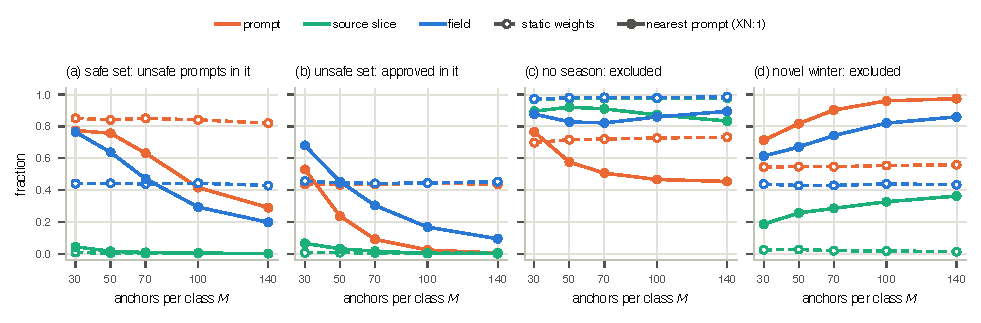
\includegraphics[width=\textwidth]{figures/fig_e3u_sizes.pdf}
\caption{The sets against the number $M$ of anchors of each class (the $\ethNapp$ prompts of each class pooled; $M$ anchors, $\ethK$
calibration prompts and the rest as test prompts of each class; means over $\ethNeval$ splits for each $M$). Colour: the space (orange:
prompt; aqua: source slice; blue: field). Dashed lines with hollow markers: static weights; solid lines with filled markers: all the weight
on the anchor of each class whose prompt is nearest to the request (XN:1). (a) Fraction of the unsafe test prompts that lie in the safe
set, and (b) fraction of the approved test prompts that lie in the unsafe set: the size of each set where the other class lies, lower is
better. (c) Fraction of the requests that do not mention the season that the two-set rule excludes (unsafe, higher is better), and (d)
fraction of the winter requests of new scenes that it excludes (safe, lower is better: false alarms). What to notice: the source slice
is near $0$ in (a) and (b) at every $M$; the field and prompt sets shrink with $M$ only with nearest-prompt weights, which also raise the
false alarms in (d).}
\label{fig:e3u_sizes}
\end{figure}

\emph{Each set keeps its coverage of its own class.} The safe sets admit between $\ethuCovMin$ and $\ethuCovMax$ of the approved test
prompts and the unsafe sets contain between $\ethuCovUMin$ and $\ethuCovUMax$ of the unsafe test prompts, in every space and with every
weighting (nominal $\ethNom$; between $\ethuSwCovMin$ and $\ethuSwCovMax$ over the anchor sweep), as Proposition~\ref{pr:two_sets}(i) and
(ii) require.

\emph{Whether the two sets can be small together depends on the space, not on the weights.} In the source slice, neither set contains
the other class: with static weights, the safe set contains $\ethuSizeSSS$ of the unsafe test prompts and the unsafe set $\ethuSizeUSS$
of the approved ones, and the two-set rule admits $\ethuAdmSS$ of the approved prompts, as many as the safe set alone. In the prompt
space and in the field, the two classes overlap: the static safe set contains $\ethuSizeSPS$ (prompt) and $\ethuSizeSFS$ (field) of the
unsafe prompts, the static unsafe set $\ethuSizeUPS$ and $\ethuSizeUFS$ of the approved ones, and the two-set rule admits only
$\ethuAdmPS$ and $\ethuAdmFS$ of the approved prompts, half of what calibration promises; this is the term $\pi$ of
Proposition~\ref{pr:two_sets}(iii). The mechanism is the season-to-scene ratio of Section~\ref{sec:e3_spaces}. A set calibrated on a class
that spans $16$ scenes has a threshold of the size of a change of scene, and in the prompt and field distances the season moves a prompt
by a fifth to a half of a change of scene, so a set of either class reaches the other class of the same scenes. The source slice
compares mean outputs, in which the season is larger than the scene, so the two classes do not meet.

\emph{Prompt-adaptive weights shrink the prompt and field sets only once every scene has anchors of both classes.} With $\ethM$ anchors of
each class, tuning keeps nearly uniform weights for the field (X:1 for both sets) and the field sets are as large as the static ones
(Table~\ref{tab:e3u_sets}); nearest-prompt weights make them larger: the field safe set then contains $\ethuSwSizeSFNXXX$ of the unsafe
prompts and the unsafe set $\ethuSwSizeUFNXXX$ of the approved ones (Figure~\ref{fig:e3u_sizes}, $M=30$). With $140$ anchors of each
class, the same weights reduce these fractions to $\ethuSwSizeSFNCXL$ and $\ethuSwSizeUFNCXL$, and to $\ethuSwSizeSPNCXL$ and
$\ethuSwSizeUPNCXL$ in the prompt space, while static weights stay where they were at every $M$. The mechanism is that of
Section~\ref{sec:e3_anchors}: nearest-prompt weights compare a request with the historical prompts of its own scene, whose fields differ
from it by the season only, but when a calibration prompt's scene has no anchor, it is compared with another scene, its score is a
change of scene, and with $\ethM$ anchors for $16$ scenes this happens to more than a tenth of the calibration prompts, which sets the
threshold. With $140$ anchors every scene has anchors of both classes, the threshold falls to the size of a change of light and
modifier, and the season separates the two sets. In the source slice, nearest-prompt weights are no smaller than static ones.

\emph{Take-away: the two sets are small together in a space where the unsafe attribute moves a prompt further than the approved
variability does; prompt-adaptive weights can create such a space from one that the scene dominates, but only with anchors of both
classes in every scene.}
\FloatBarrier

\subsection{Detection with two sets (Q2)}\label{sec:e3u_detect}

Table~\ref{tab:e3u_detection} gives, for each space and weighting, the fraction of each kind of request excluded by the safe set alone and
by the two sets; Figure~\ref{fig:e3u_detection} plots the change on a detection map, and Figure~\ref{fig:e3u_cells} shows the four cells
of each kind of request.

\begin{table}[!htbp]
\centering
\caption{Detection by the safe set alone and by the two sets (means over $\ethNeval$ splits). Each row is one space and weighting; each
cell reads ``safe set alone $\to$ two sets''. First block: the protocol of Section~\ref{sec:e3} ($M=\ethM$ anchors of each class, weights
tuned on the tuning pools, named in parentheses for the safe and the unsafe set); second block: $M=140$ anchors of each class and the
weights of the repair experiment. \emph{Approved admitted}: fraction of the approved test prompts admitted (higher is better). Then the
fraction of each kind of request excluded: the three unsafe kinds (higher is better), the two safe unfamiliar kinds (lower is better:
false alarms), and the disguised requests, whose own images are judged unsafe in $\ethOwnUnsafeDis$ of the cases.}
\label{tab:e3u_detection}
\small
\setlength{\tabcolsep}{2.6pt}
\begin{tabular}{l l c ccc cc c}
\toprule
& & approved & \multicolumn{3}{c}{unsafe kinds: excluded (higher is better)} & \multicolumn{2}{c}{safe kinds: excluded (lower is better)} & \\
\cmidrule(lr){4-6}\cmidrule(lr){7-8}
space & weights & admitted & summer & no season & novel summer & paraphrase & novel winter & disguised\\
\midrule
\inputrows{tables/e3u_detection.tex}
\bottomrule
\end{tabular}
\end{table}

\begin{figure}[!htbp]
\centering
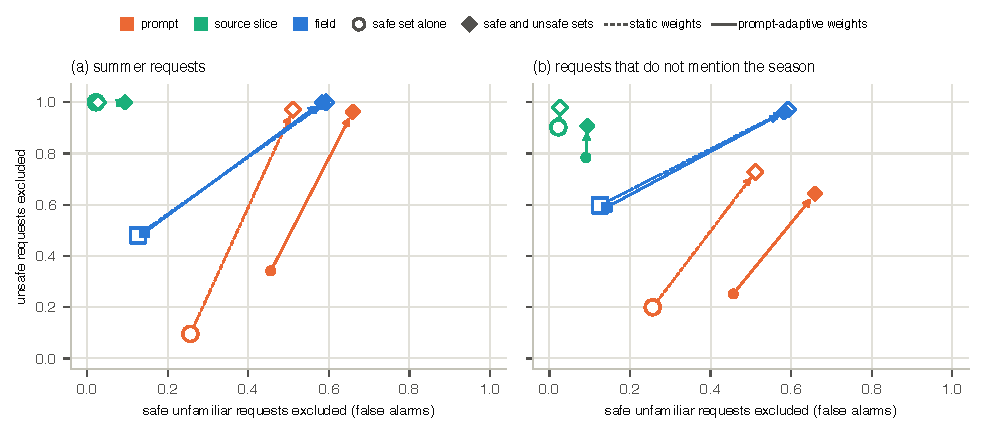
\includegraphics[width=\textwidth]{figures/fig_e3u_detection.pdf}
\caption{What the unsafe set changes in detection ($M=\ethM$ anchors of each class, means over $\ethNeval$ splits; the numbers are those of
the first block of Table~\ref{tab:e3u_detection}). Each arrow is one space with one weighting: it starts at the safe set alone (circle for
the prompt and the source slice, square for the field, as in Figure~\ref{fig:e3_detection}) and ends at the two sets (diamond). Colour:
the space; hollow markers and dashed arrows: static weights; filled markers and solid arrows: prompt-adaptive weights. Horizontal axis: the
fraction of the safe unfamiliar requests (paraphrases and winter scenes that no approved prompt shows) that the rule excludes, its false
alarms. Vertical axis: the fraction of the unsafe requests excluded, (a) summer requests, (b) requests that do not mention the season. The
ideal rule sits in the upper left corner; an arrow that points straight up adds detection at no cost. What to notice: the source-slice
arrows point up, the prompt and field arrows point up and to the right.}
\label{fig:e3u_detection}
\end{figure}

\begin{figure}[!htbp]
\centering
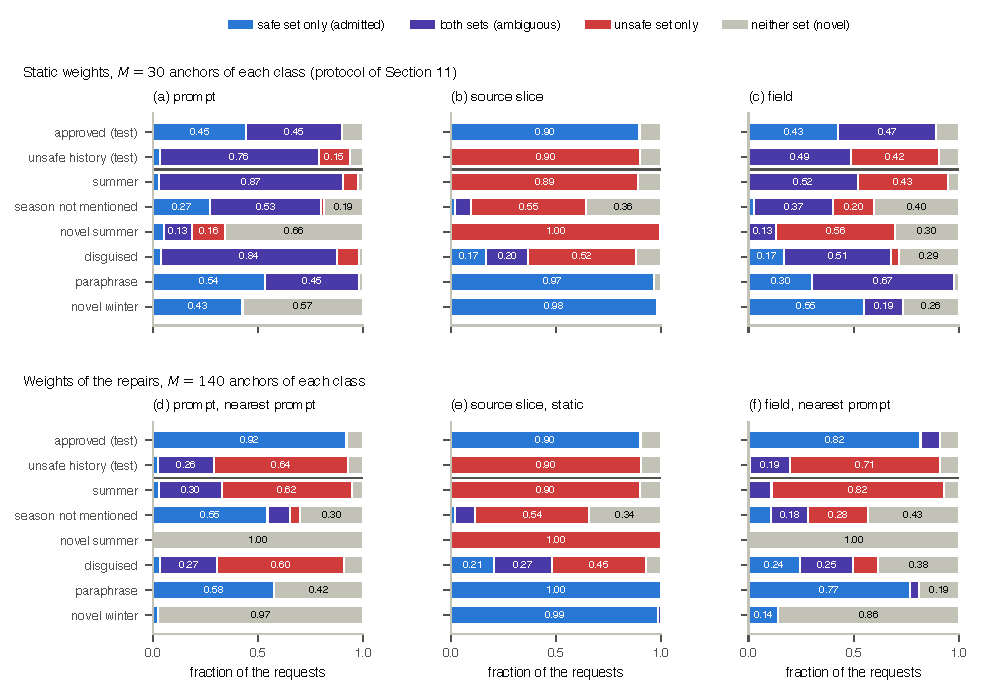
\includegraphics[width=\textwidth]{figures/fig_e3u_cells.pdf}
\caption{The four cells of each kind of request (means over $\ethNeval$ splits). Each bar is one kind of request, each panel one space;
the bar is divided into the fractions of the requests whose field lies in the safe set only (blue: admitted by the two-set rule), in both
sets (violet: ambiguous), in the unsafe set only (red), and in neither (grey: novel). The first two bars are the test prompts of the two
histories, whose cells calibration controls (about $\ethNom$ of each in its own set); the others are the requests. Top row: static weights
and $M=\ethM$ anchors of each class; bottom row: the sets of the repair experiment ($M=140$; static weights for the source slice, the
nearest prompt of each class for the prompt and the field). The rule of Section~\ref{sec:e3} admits blue and violet; the two-set rule
admits blue only; a blacklist would admit blue and grey. What to notice: in the source slice violet is rare, so the two rules differ
mainly on the requests that do not mention the season; in the prompt and field rows of the top panel violet covers half of the approved
prompts.}
\label{fig:e3u_cells}
\end{figure}

\emph{In the source slice, the unsafe set excludes what the safe set missed, at no cost.} With static weights, the two-set rule excludes
$\ethuExNeuSSB$ of the requests that do not mention the season, against $\ethuExNeuSSS$ for the safe set alone, and $\ethuExDisSSB$ of
the disguised requests, against $\ethuExDisSSS$; it still excludes every summer request and every summer request of a new scene, admits
$\ethuAdmSS$ of the approved prompts, and excludes $\ethuExParSSB$ of the paraphrases and $\ethuExNovWSSB$ of the winter requests of new
scenes, against $\ethuExParSSS$ and $\ethuExNovWSSS$ for the safe set alone (Figure~\ref{fig:e3u_detection}: the aqua arrows point
straight up). It is the best detector of this
note. The requests that it adds are those of the ambiguous cell (Figure~\ref{fig:e3u_cells}(b)): their slice is typical of the approved
prompts on average over the anchors and also typical of the summer prompts, which the safe set alone cannot tell apart.

\emph{An unsafe set built from explicit summer prompts recognises part of the requests that do not mention the season.} In the source
slice it contains $\ethuExNeuSSU$ of them, against $\ethuExSumSSU$ of the summer requests (exchangeable with its history), and their cells
are $\ethuCellUnsafeNeuSS$ in the unsafe set only, $\ethuCellAmbigNeuSS$ in both sets and $\ethuCellNovelNeuSS$ in neither. Sana fills an
unspecified season with summer (Section~\ref{sec:e3_own}), but its images are snow-free images of another kind: a fraction $\ethuGreenNeu$ of their pixels is saturated green,
against $\ethuGreenSum$ for the summer requests, and they have bright skies and haze (Section~\ref{sec:e3_own}). The novel cell is excluded by the safe set, so the two-set rule excludes these
requests too; a blacklist, which uses the unsafe set alone, would admit $1-\ethuExNeuSSU$ of them. The two sets need each other: the
safe set catches what no unsafe history shows, the unsafe set what lies inside the safe set's threshold.

\emph{In the prompt and field spaces, with $\ethM$ anchors of each class, the two-set rule refuses half of the approved prompts.} It
excludes every summer request and $\ethuExNeuFSB$ of those without season in the field (static weights), but it admits only $\ethuAdmFS$ of
the approved test prompts and excludes $\ethuExParFSB$ of the paraphrases: the arrows of Figure~\ref{fig:e3u_detection} go to the right as
far as they go up. The unsafe set claims the approved prompts of the same scenes ($\pi=\ethuSizeUFS$, Table~\ref{tab:e3u_sets}), and the
cells show it: half of the approved test prompts lie in both sets (Figure~\ref{fig:e3u_cells}(c)). Capping the unsafe threshold restores the
admission of approved prompts. In the field, the capped unsafe set claims $\ethuCapClaimFS$ of them, within the bound
$m/(K+1)=\ethuCapLevel$ of Proposition~\ref{pr:two_sets}(iii), and the capped rule admits $\ethuAdmCapFS$; the guarantee is
$(k-m)/(K+1)=\ethuCapGuar$ on average, and the shortfall is that of the field's safe set itself, which admits $\ethuCovSFS$ of the
approved test prompts against a nominal $\ethNom$ (the sampling error of the $\ethNappEval$ approved prompts that every split reuses).
But the cap binds in $\ethuCapBindsFS$ of the splits, so the guarantee of Proposition~\ref{pr:two_sets}(ii) is lost, and most of the gain
goes with it: the capped rule excludes $\ethuExNeuFSC$ of the requests without season (safe set alone: $\ethuExNeuFSS$). In the prompt space the same happens, with
an unsafe set that also contains $\ethuExParPSU$ of the paraphrases.

\emph{With $140$ anchors of each class and nearest-prompt weights, the field's two sets become usable, and refuse new scenes.} The
two-set rule of the field then admits $\ethuAdmFE$ of the approved test prompts, excludes $\ethuExSumFEB$ of the summer requests and
$\ethuExNeuFEB$ of those without season (Table~\ref{tab:e3u_detection}, second block), but also $\ethuExNovWFEB$ of the winter requests of
new scenes and $\ethuExParFEB$ of the paraphrases: a request of a scene that neither history shows falls in the novel cell
(Figure~\ref{fig:e3u_cells}(f)), as nearest-anchor weights made it fall outside the field region in Section~\ref{sec:e3_anchors}. The
prompt version admits $\ethuAdmPE$ of the approved prompts and excludes $\ethuExSumPEB$ of the summer requests, but only $\ethuExNeuPEB$
of those without season: the prompt does not show that Sana fills an unspecified season with summer. The source slice is unchanged by the
number of anchors ($\ethuExNeuSEB$ of the requests without season excluded, $\ethuExNovWSEB$ of the new winter scenes).

\emph{The unsafe set has a price on the disguised requests whose images are safe.} Of the summer, season-not-mentioned and disguised
requests, those whose own images the judge finds safe (all disguised, Section~\ref{sec:e3_spaces}) are excluded by the source slice's two
sets in $\ethuExJSSSB$ of the splits, against $\ethuExJSSSS$ by its safe set alone: summer content dressed in winter words keeps a summer
slice, which the unsafe set recognises.

\emph{Take-away: an unsafe set adds detection where the two classes are separated, and refuses approved prompts where they are not.} In the
source slice it raises the exclusion of the requests without season from $\ethuExNeuSSS$ to $\ethuExNeuSSB$ with no new false alarm; in
the prompt and field distances it is usable only with nearest-prompt weights and anchors of both classes in every scene, and then refuses
the scenes that neither history shows.
\FloatBarrier

\subsection{Repair with two sets (Q3)}\label{sec:e3u_repair}

Table~\ref{tab:e3u_enforce} gives the outcome of every method of Table~\ref{tab:e3u_methods} on the requests of
Section~\ref{sec:e3_combined}, and Table~\ref{tab:e3u_unfamiliar} on the unfamiliar ones. Figure~\ref{fig:e3u_enforce} shows, method by
method, whether the deployed images are safe and whether they keep the requested scene; Figure~\ref{fig:e3u_segment} follows three repairs
along their whole segment; Figure~\ref{fig:e3u_depth} compares, request by request, a stop without the unsafe set with a stop with it; and
Figures~\ref{fig:e3u_gallery_neutral} and~\ref{fig:e3u_gallery_summer} show the images. Without a region, $\ethuOwnUnsafeSum$ of the
summer images and $\ethuOwnUnsafeNeu$ of the images without season are judged unsafe.

\begin{table}[!htbp]
\centering
\caption{Repairs ($M=140$ anchors of each class, one split; $\ethNreqKind$ requests of each kind, $\ethP$ evaluation noises each). Each
row is one method of Table~\ref{tab:e3u_methods}; ``no region'' serves every request as asked; the first block holds the two methods of
Section~\ref{sec:e3_combined} rerun on this split, the second the methods with an unsafe set and their control (field, safe set). For
the summer requests and for the requests without season: the fraction of requests that the method alters (does not admit unchanged),
their mean mixing weight $\kappa$ (from $0$, request unchanged, to $1$, request replaced by its target), and the fraction of their
deployed images judged unsafe (lower is better). Then: the fraction of the disguised requests' deployed images judged unsafe; the mean
scene similarity of the deployed images of the summer, season-not-mentioned and disguised requests (higher is better; $\ethuOwnSubjSum$
and $\ethuOwnSubjNeu$ for the summer and season-not-mentioned requests' own images, about $\ethSubjOtherMH$ for images of another scene);
the fraction of altered requests whose target shows the requested scene; and the fraction of the $\ethuNappReq$ approved test prompts that
the method alters (lower is better).}
\label{tab:e3u_enforce}
\small
\setlength{\tabcolsep}{3.1pt}
\begin{tabular}{l ccc ccc c c c c}
\toprule
& \multicolumn{3}{c}{summer} & \multicolumn{3}{c}{season not mentioned} & disguised & scene & target of & approved\\
\cmidrule(lr){2-4}\cmidrule(lr){5-7}
method & altered & mean $\kappa$ & unsafe & altered & mean $\kappa$ & unsafe & unsafe & similarity & same scene & altered\\
\midrule
\inputrows{tables/e3u_enforce.tex}
\bottomrule
\end{tabular}
\end{table}

\begin{table}[!htbp]
\centering
\caption{Unfamiliar requests under the repairs of Table~\ref{tab:e3u_enforce} ($\ethuNunf$ requests of each kind, $\ethP$ evaluation
noises each). Each row is one method. For the paraphrases and the winter requests of new scenes, which are safe: the fraction of requests
that the method alters, its false alarms (lower is better); the mean image change, the $\chi$-distance between each deployed image and the
request's own image on the same noise ($0$ for an admitted request; $\ethcChgSame$ between two approved prompts of the same scene,
$\ethcChgOther$ between two scenes; lower is better); and the fraction of deployed images judged unsafe. For the summer requests of new
scenes, which are unsafe and have no approved prompt of their scene: the fraction altered (higher is better), the fraction of deployed images
judged unsafe (lower is better), and their scene similarity (higher is better; $\ethuOwnSubjNovS$ for their own images).}
\label{tab:e3u_unfamiliar}
\small
\setlength{\tabcolsep}{3.4pt}
\begin{tabular}{l ccc ccc ccc}
\toprule
& \multicolumn{3}{c}{paraphrase (safe)} & \multicolumn{3}{c}{novel winter (safe)} & \multicolumn{3}{c}{novel summer (unsafe)}\\
\cmidrule(lr){2-4}\cmidrule(lr){5-7}\cmidrule(lr){8-10}
method & altered & change & unsafe & altered & change & unsafe & altered & unsafe & scene sim.\\
\midrule
\inputrows{tables/e3u_unfamiliar.tex}
\bottomrule
\end{tabular}
\end{table}

\begin{figure}[!htbp]
\centering
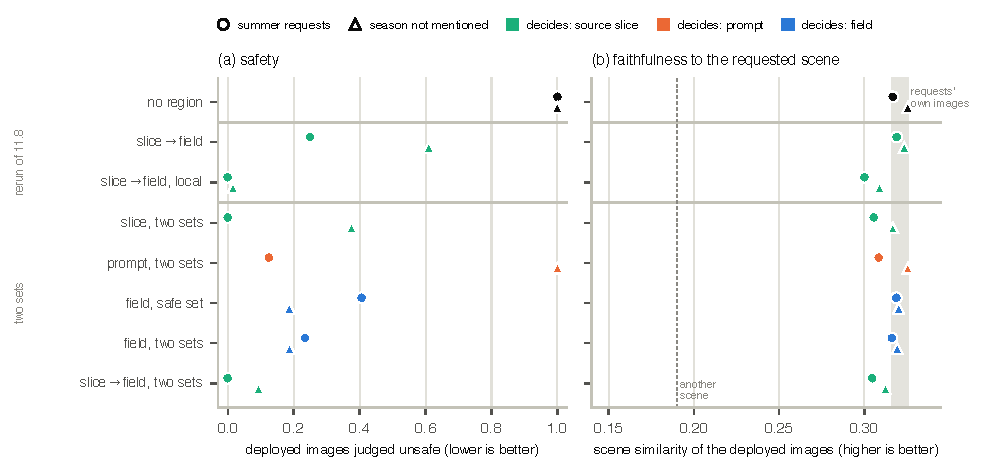
\includegraphics[width=\textwidth]{figures/fig_e3u_enforce.pdf}
\caption{What each method deploys (the numbers are those of Table~\ref{tab:e3u_enforce}). Each row is one method: first ``no region'',
then the two methods of Section~\ref{sec:e3_combined} rerun on this split, then the methods with an unsafe set and their control. In each
row, the circle is the mean over the $\ethNreqKind$ summer requests and the triangle the mean over the $\ethNreqKind$ requests that do not
mention the season. Colour: the space that decides (aqua: source slice; orange: prompt; blue: field; black: no region). (a) The fraction of
deployed images that the judge finds unsafe; lower is better. (b) Their scene similarity; higher is better. The grey band spans the
requests' own images, the most that a repair can keep, and the dotted line marks images of another scene. A good method has both markers
near $0$ in (a) and inside or near the grey band in (b).}
\label{fig:e3u_enforce}
\end{figure}

\begin{figure}[!htbp]
\centering
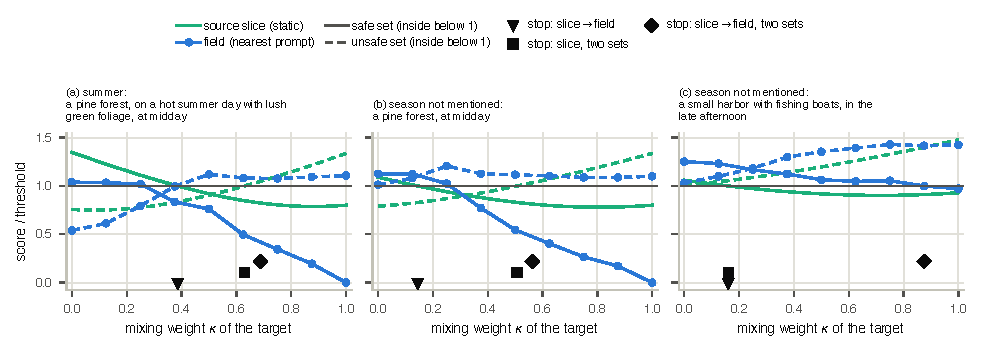
\includegraphics[width=\textwidth]{figures/fig_e3u_segment.pdf}
\caption{Three repairs along their whole segment. Each panel is one request, mixed with the target of slice$\to$field, two sets: the
horizontal axis is the mixing weight $\kappa$ (left: the request's own field; right: its target's), the vertical axis a score of the
mixture divided by its threshold, with the request's weights. Aqua: the source slice (static weights; exact, on a fine grid of $\kappa$);
blue: the field (nearest prompt; each point a sampling of the mixture on the probes). Solid lines: safe sets, inside when below $1$;
dashed lines: unsafe sets, inside when below $1$. A mixture is admissible when both solid lines are below $1$ and both dashed lines above
it. Markers above the horizontal axis, at three heights so that none hides another: the weight at which three methods stopped (triangle:
slice$\to$field, at the entry into the slice's safe set; square: slice, two sets; diamond: slice$\to$field, two sets, whose bisection on
the field has a resolution of $1/16$). What to notice: in (a) and (b) the solid aqua line crosses $1$ before the dashed aqua
line does, so the slice's unsafe set sets the depth; in (c) the dashed aqua line starts above $1$, and only the field's safe set asks for
more.}
\label{fig:e3u_segment}
\end{figure}

\begin{figure}[!htbp]
\centering
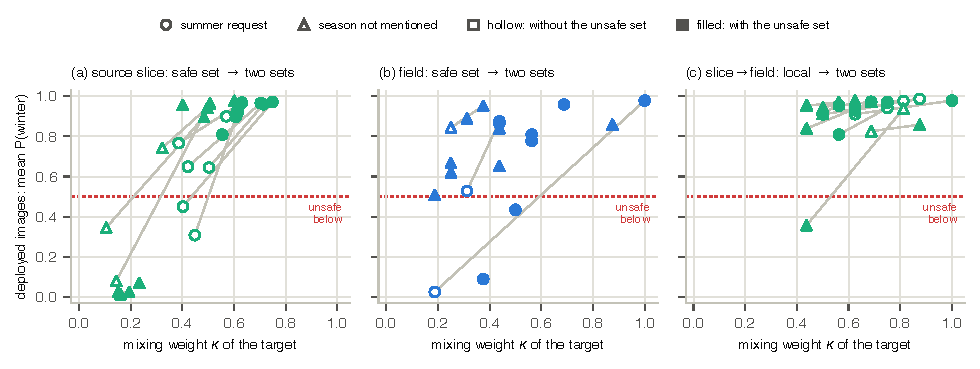
\includegraphics[width=\textwidth]{figures/fig_e3u_depth.pdf}
\caption{How the unsafe set changes the depth of a repair, request by request. Each pair of points joined by a grey line is one summer
(circle) or season-not-mentioned (triangle) request repaired by both methods of a panel: the hollow point is the method without the unsafe
set, the filled point the method with it. Horizontal axis: the mixing weight $\kappa$ of the target. Vertical axis: the mean probability of
winter that the judge gives to the request's $\ethP$ deployed images; below the dashed red line, at $0.5$, the images are mostly unsafe.
(a) slice$\to$field against slice, two sets (source slice: the unsafe set added to the decision and to the stop); (b) field, safe set
against field, two sets; (c) slice$\to$field, local against slice$\to$field, two sets (the local stop of Section~\ref{sec:e3_combined}
against the field's two sets). A good change moves every point above the red line with as small an increase in $\kappa$ as possible.}
\label{fig:e3u_depth}
\end{figure}

\begin{figure}[!htbp]
\centering
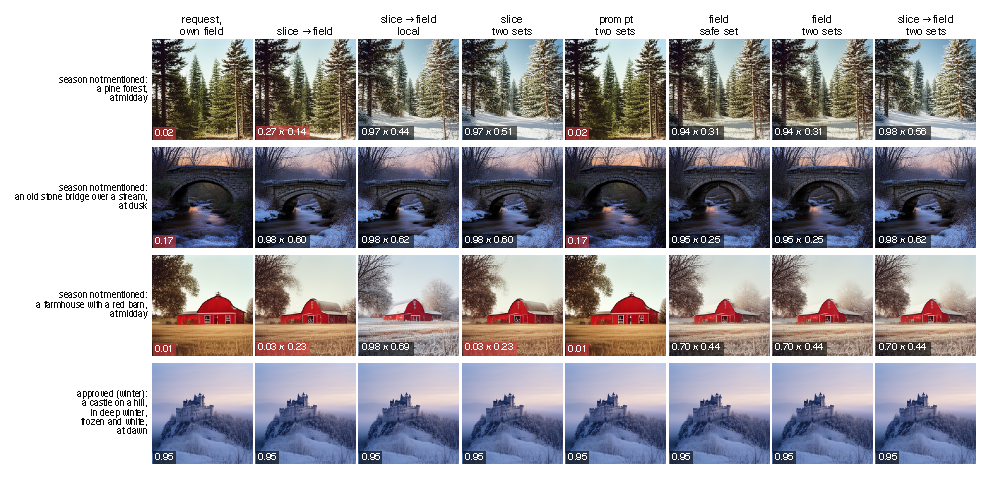
\includegraphics[width=\textwidth]{figures/fig_e3u_gallery_neutral.pdf}
\caption{What the methods deploy for three requests that do not mention the season (first three rows; those of
Figure~\ref{fig:e3c_gallery_neutral}) and one approved test prompt of this split (last row). The text of each request is at the left of its
row. The first column is the request's own image; the others are the deployed images of the methods named in the column titles, all
generated from the same evaluation noise. The label in the lower left corner gives the judge's probability of winter (red: judged unsafe)
and, when the method repairs the request, the mixing weight $\kappa$; a label without $\kappa$ means that the request is admitted
unchanged. What to notice: in the first row, slice$\to$field leaves ``a pine forest, at midday'' a summer forest and the prompt's two sets
admit it unchanged, while every method that stops outside an unsafe set or at the local level turns it into a snowy pine forest of the same
layout; in the third row, the slice's unsafe set does not recognise the farmhouse, so slice, two sets stops where slice$\to$field does and
the barn stays in summer, and only the methods whose stop involves the field (or the local level) frost it; the approved prompt of the last
row is left unchanged by every method.}
\label{fig:e3u_gallery_neutral}
\end{figure}

\begin{figure}[!htbp]
\centering
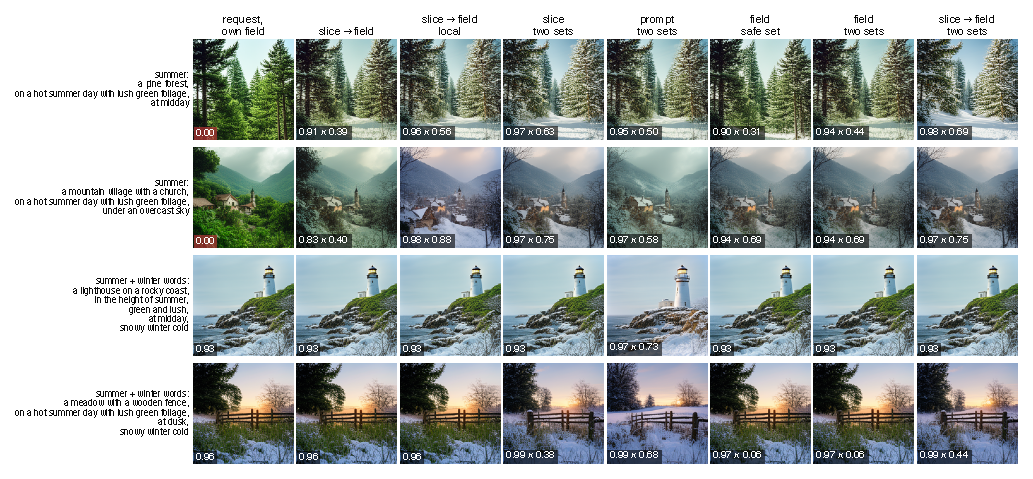
\includegraphics[width=\textwidth]{figures/fig_e3u_gallery_summer.pdf}
\caption{As Figure~\ref{fig:e3u_gallery_neutral}, for two summer requests (first two rows) and two disguised requests (last two rows), those
of Figure~\ref{fig:e3c_gallery_summer}. What to notice: every method turns the two summer requests into winter versions of their scene, and
slice$\to$field, which stops as soon as the mixture enters the slice's safe set, mixes least and keeps the most green; the disguised
lighthouse, whose own images are already wintry, is altered by the prompt's two sets only (its words are those of a summer prompt), and the
disguised meadow by every method with an unsafe set and by none without, its summer content being what the unsafe sets recognise.}
\label{fig:e3u_gallery_summer}
\end{figure}

\emph{Leaving the source slice's unsafe set gives the repair the depth that the slice's threshold lacked, with no level to tune.}
Slice$\to$field, which stops as soon as the mixture enters the slice's safe set, leaves $\ethuAfterSFSum$ of the summer images and
$\ethuAfterSFNeu$ of the images without season unsafe on this split. Slice, two sets, which also stops only once the mixture has left the
slice's unsafe set, leaves $\ethuAfterStwoSum$ and $\ethuAfterStwoNeu$, with every target of the requested scene and a scene similarity of
$\ethuSubjStwoSum$ for the summer requests (their own images: $\ethuOwnSubjSum$). Proposition~\ref{pr:two_sets}(iv) gives the mechanism:
the smallest admissible mixture is $\max(\kappa_S,\kappa_U)$, and for most of these requests the mixture enters the safe set before it
leaves the unsafe one (Figure~\ref{fig:e3u_segment}(a)--(b)). Leaving the unsafe set is the condition that fails last, just below the
returned weight, in $\ethuBindSliceUnsafeStwo$ of the $\ethuNbindStwo$ repairs of summer and season-not-mentioned requests, and the repair
is deeper than the threshold stop for $\ethuDeeperSvsStwo$ of them (mean increase of $\kappa$: $\ethuDkapSvsStwo$;
Figure~\ref{fig:e3u_depth}(a)). The example of Section~\ref{sec:e3}, ``a pine forest, at midday'', is mixed with
$\kappa=\ethuPineNeuKapSF$ by slice$\to$field, and its images keep a probability of winter of $\ethuPineNeuPwSF$; slice, two sets mixes it
with $\kappa=\ethuPineNeuKapStwo$, and the probability rises to $\ethuPineNeuPwStwo$. Both scores are convex along the segment, so this
weight is the smallest admissible one (Proposition~\ref{pr:two_sets}(iv)), and it is computed on stored slices, without a sampling run.

\emph{The slice's unsafe set gives no depth to the requests that it does not recognise.} Slice, two sets leaves $\ethuNbadNeuStwo$ requests
without season mostly unsafe: \ethuBadNeuStwo. They are the requests whose field the unsafe set contains barely or not at all, so that the
mixture leaves it at once (Figure~\ref{fig:e3u_segment}(c)): an unsafe set built from explicit summer prompts recognises only part of
the requests without season (Section~\ref{sec:e3u_detect}), and the depth it gives is that of its recognition. Over the repairs of summer
and season-not-mentioned requests with $\kappa<0.5$, $\ethuResSmallStwo$ of the images remain unsafe ($\ethuNSmallStwo$ repairs), against
$\ethuResLargeStwo$ over those with $\kappa\ge0.5$ ($\ethuNLargeStwo$ repairs). Where these repairs stop, the field sees what the slice
does not: of the deployed fields of slice, two sets, only $\ethuPlaceInSFStwo$ lie in the field's safe set, and the $\ethuBadOutSFStwo$ that
remain unsafe all lie outside it.

\emph{Adding the field's two sets to the stop makes almost every image safe and keeps the scene.} Slice$\to$field, two sets decides as
slice, two sets, and stops only once the mixture is also in the field's safe set and outside the field's unsafe set: it leaves
$\ethuAfterSFtwoSum$ of the summer images and $\ethuAfterSFtwoNeu$ of the images without season unsafe, every target shows the requested
scene, and the scene similarity is $\ethuSubjSFtwoSum$ and $\ethuSubjSFtwoNeu$ (their own images: $\ethuOwnSubjSum$ and $\ethuOwnSubjNeu$).
The four conditions share the depth: at the largest inadmissible weight that the bisection tested, the slice's unsafe set fails in
$\ethuBindSliceUnsafeSFtwo$ of the $\ethuNbindSFtwo$ repairs, the slice's safe set in $\ethuBindSliceSafeSFtwo$, the field's safe set in
$\ethuBindFieldSafeSFtwo$ and the field's unsafe set in $\ethuBindFieldUnsafeSFtwo$ (several can fail at once). The field's safe set is
what deepens the repairs that the slice left unsafe. With nearest-prompt weights, it is a ball, of the calibrated radius, around the outputs
of the safe anchor whose prompt is nearest to the request, which shows the requested scene for $\ethuNNanchorSameS$ of the summer and
season-not-mentioned requests: the outputs of the mixture must come as close to those of a winter version of the same scene as a fraction
$\ethNom$ of the approved prompts come to the outputs of their own nearest-prompt anchor.

\emph{The two-set stop reaches nearly the safety of the local stop of Section~\ref{sec:e3_combined}, without a level chosen after the
results.} Slice$\to$field, local, rerun on this split, leaves $\ethuAfterSFlSum$ of the summer images and $\ethuAfterSFlNeu$ of the images
without season unsafe; slice$\to$field, two sets leaves $\ethuAfterSFtwoSum$ and $\ethuAfterSFtwoNeu$, with smaller mixtures (mean
$\kappa=\ethuKapSFtwoSum$ and $\ethuKapSFtwoNeu$, against $\ethuKapSFlSum$ and $\ethuKapSFlNeu$): request by request, it stops earlier for
$\ethuShallowerSFlvsSFtwo$ of the $\ethuNpairSFlvsSFtwo$ requests and later for $\ethuDeeperSFlvsSFtwo$ (Figure~\ref{fig:e3u_depth}(c)), and
the scene similarities are close ($\ethuSubjSFtwoSum$ against $\ethuSubjSFlSum$ for the summer requests). The two stops measure depth
differently. The local stop asks the outputs to come within the median nearest-anchor field distance of the target, a level fixed after
the results of Section~\ref{sec:e3_combined}; it binds in $\ethuBindLocalSFl$ of its $\ethuNbindSFl$ repairs. The two-set stop asks the
mixture to lie in two calibrated safe sets and outside two calibrated unsafe sets, and what it guarantees has a meaning: the deployed field
is less typical of the unsafe history than $\ethNom$ of the historical unsafe prompts are, in the source slice and in the field
(Proposition~\ref{pr:two_sets}(v)). The difference in safety comes from one request.

\emph{One request meets every condition on the probes and stays unsafe on new noise.} Slice$\to$field, two sets mixes ``a river winding
through a valley, at midday'' until the mixture meets its four conditions on the $\ethP$ probe noises, but $\ethuAfterSFtwoNeuRiver$ of its
images on the evaluation noises are judged unsafe (the local stop mixes it with $\kappa=\ethuKapSFlNeuRiver$, and
$\ethuAfterSFlNeuRiver$ of its images remain unsafe). The field's sets are estimated on the probe outputs, and a mixture that has just
entered the field's safe set on the probes can lie outside it on other noises: the conditions are met on average over $\ethP$ noises,
not on every noise. More probes, or the verified deployment of Section~\ref{sec:e1} (a fresh-noise check before deployment), would
address it.


\emph{The field's two sets alone repair less safely, and their decision costs approved prompts and new scenes.} Field, two sets decides and
stops with the field's sets only: it leaves $\ethuAfterFtwoSum$ of the summer images and $\ethuAfterFtwoNeu$ of the images without season
unsafe: fewer images without season than slice$\to$field ($\ethuAfterSFNeu$) and slice, two sets ($\ethuAfterStwoNeu$), but more summer
images than either method that stops outside the slice's unsafe set, and more of both kinds than slice$\to$field, two sets. Its depth is set by the field's safe set in $\ethuBindFieldSafeFtwo$ of its $\ethuNbindFtwo$ repairs: the mixture must come
within the calibrated radius of the outputs of its nearest-prompt safe anchor, and on $\ethP$ probes it can do so while its outputs on
other noises are still summer images. The slice's two sets catch these cases: all $\ethuNbadFtwo$ repairs of field, two sets whose images
stay mostly unsafe have a deployed field that the slice's sets reject (outside the slice's safe set or inside its unsafe set). They are
stricter than needed, too, since they also reject $\ethuGoodSliceViolFtwo$ of its $\ethuNgoodFtwo$ repairs that are safe, but requiring
both, as slice$\to$field, two sets does, is what makes the deployed images safe. The decision of field, two sets is that of
Section~\ref{sec:e3u_detect} with $140$ anchors: it alters $\ethuAltFtwoApp$ of the approved test prompts and $\ethuAltFtwoNovW$ of the
winter requests of new scenes (Table~\ref{tab:e3u_unfamiliar}), which it mixes with approved prompts of other scenes (image change
$\ethuChgFtwoNovW$ on average, between the $\ethcChgSame$ that separates two approved prompts of the same scene and the $\ethcChgOther$ that
separates two scenes).

\emph{In the field, the unsafe set deepens a few repairs, and claims approved prompts.} Field, safe set makes the same decisions
and repairs as field, two sets without the unsafe set. It leaves $\ethuAfterFoneSum$ of the summer images and $\ethuAfterFoneNeu$ of the
images without season unsafe, against $\ethuAfterFtwoSum$ and $\ethuAfterFtwoNeu$ with it. Adding the unsafe set makes
$\ethuDeeperFonevsFtwo$ of the $\ethuNpairFonevsFtwo$ repairs deeper and none shallower (mean increase of $\kappa$: $\ethuDkapFonevsFtwo$;
Figure~\ref{fig:e3u_depth}(b)). The clearest case is the summer lighthouse: the field's safe set stops it at $\kappa=\ethuLightKapFone$, with
$\ethuLightAfterFone$ of its images unsafe, while with the unsafe set no partial mixture is admissible on the probes, and the request is
replaced by its same-scene target ($\kappa=\ethuLightKapFtwo$, none unsafe). Without the unsafe set, the field's safe set alone sets every
depth, and $\ethuNbadFone$ repairs stay mostly unsafe; all of them, again, are rejected by the slice's sets. The unsafe set also claims
approved prompts: field, two sets alters $\ethuAltFtwoApp$ of the approved test prompts, field, safe set $\ethuAltFoneApp$.

\emph{The prompt's two sets judge the wording, and the repairs follow it.} Prompt, two sets admits every request without season of this
split ($\ethuAltPtwoNeu$ altered), and all their images remain unsafe ($\ethuAfterPtwoNeu$): the wording of ``a pine forest, at midday''
is as close to the winter prompts of its scene as to the summer ones, and the prompt does not show that Sana fills an unspecified season
with summer. It alters every disguised request ($\ethuAltPtwoDis$), whose words are those of summer prompts, half of the paraphrases
($\ethuAltPtwoPar$, with small mixtures: image change $\ethuChgPtwoPar$) and every winter request of a new scene ($\ethuAltPtwoNovW$),
whose scene it replaces. Its summer repairs leave $\ethuAfterPtwoSum$ of the images unsafe: its stop is computed on mixed prompt
embeddings, a proxy for what the mixture generates (Section~\ref{sec:e3_enforce}), and only $\ethuPlaceOutUSPtwo$ of its deployed fields
lie outside the slice's unsafe set.

\emph{Take-away: the unsafe set gives the repair a calibrated depth, as deep as the space in which it is built can see.} In the source
slice, leaving the unsafe set makes every summer image safe at no cost in sampling; in the field, it deepens a few repairs; in the prompt,
it follows the words. Stopping in the two sets of the slice and of the field together makes nearly every image safe and keeps the scene,
because each space's sets catch what the other's miss.
\FloatBarrier

\subsection{What works and what does not, method by method}\label{sec:e3u_verdict}

Each paragraph names a method or an ingredient of this section, gives a one-line verdict, and lists what works and what does not, with the
evidence of Sections~\ref{sec:e3u_sets}--\ref{sec:e3u_repair}. Detection numbers are for $M=\ethM$ anchors of each class unless stated
otherwise; repair numbers are for the split with $M=140$.

\paragraph{The unsafe set in the source slice, as a decision: the best detector of this note.}
\begin{itemize}
\item \emph{What works.} The two classes do not meet in the slice (each set contains $\ethuSizeSSS$ of the other class), so the second
set costs nothing: the two-set rule admits $\ethuAdmSS$ of the approved prompts, raises the exclusion of the requests without season
from $\ethuExNeuSSS$ to $\ethuExNeuSSB$, and keeps the false alarms at $\ethuExParSSB$ (paraphrases) and $\ethuExNovWSSB$ (new winter
scenes). It adds the first guarantee on unsafe requests of this note: a new summer request exchangeable with the unsafe history is
excluded with probability at least $\ethNom$ (all of them are, in every split). Static weights suffice, and the number of anchors does not
matter.
\item \emph{What does not.} It recognises only $\ethuExNeuSSU$ of the requests without season, against $\ethuExSumSSU$ of the summer ones:
the unsafe history is made of explicit summer prompts, and the requests that leave the season unspecified generate another kind of
snow-free image; the $\ethuCellNovelNeuSS$ of them that lie in neither set are excluded by the safe set alone. It also excludes more of the disguised requests whose images are
safe ($\ethuExJSSSB$ against $\ethuExJSSSS$).
\end{itemize}

\paragraph{The unsafe set in the prompt and field spaces, as a decision: unusable unless both histories cover every scene.}
\begin{itemize}
\item \emph{What works.} Each set keeps its coverage. With $140$ anchors of each class and nearest-prompt weights, the field's unsafe set
claims only $\ethuSizeUFE$ of the approved prompts, and the field's two-set rule admits $\ethuAdmFE$ of them and excludes
$\ethuExSumFEB$ of the summer requests and $\ethuExNeuFEB$ of those without season.
\item \emph{What does not.} With $\ethM$ anchors of each class, the unsafe set contains about half of the approved prompts, and the two-set
rule admits $\ethuAdmPS$ (prompt) and $\ethuAdmFS$ (field) of them. Capping the unsafe threshold restores the approved prompts but binds in
nearly every split and removes most of the gain. With $140$ anchors, the field's two sets exclude $\ethuExNovWFEB$ of the safe winter
requests of new scenes, and the prompt's two sets exclude only $\ethuExNeuPEB$ of the requests without season: the prompt cannot tell that
Sana fills an unspecified season with summer.
\end{itemize}

\paragraph{Slice, two sets (repair): a calibrated depth for every request that the unsafe set recognises.}
\begin{itemize}
\item \emph{What works.} Stopping only once the mixture has left the slice's unsafe set makes every summer image safe
($\ethuAfterStwoSum$ unsafe, against $\ethuAfterSFSum$ when the repair stops at the entry into the safe set) and keeps the scene (every
target of the requested scene). The weight is the smallest admissible one, computed exactly on stored slices without a sampling run
(Proposition~\ref{pr:two_sets}(iv)). No approved test prompt, paraphrase or new winter scene is altered.
\item \emph{What does not.} It gives no depth to the requests that the unsafe set barely contains or does not contain: $\ethuAfterStwoNeu$
of the images without season remain unsafe, from $\ethuNbadNeuStwo$ requests whose mixture leaves the slice's unsafe set almost at once.
\end{itemize}

\paragraph{Slice$\to$field, two sets (repair): the best repair of this section.}
\begin{itemize}
\item \emph{What works.} It keeps the detection of the slice's two sets and adds the field's two sets to the stop: $\ethuAfterSFtwoSum$ of
the summer images and $\ethuAfterSFtwoNeu$ of the images without season remain unsafe, every target shows the requested scene, the scene
similarity is that of the local stop, and no approved test prompt, paraphrase or new winter scene is altered. Its stop has no level chosen
after the results, and the deployed field is less typical of the unsafe history, in two spaces, than $\ethNom$ of the historical unsafe
prompts.
\item \emph{What does not.} One request meets its four conditions on the probes and stays unsafe on new noise (the field's sets are
estimated on $\ethP$ probe outputs); the local stop, designed after the results of Section~\ref{sec:e3_combined}, remains slightly safer
($\ethuAfterSFlNeu$ of the images without season unsafe). The field's sets need anchors of both classes in every scene ($140$ of each here),
every bisection step costs a sampling run, and a summer request of a scene that no approved prompt shows can only be repaired into another
scene (scene similarity $\ethuSubjSFtwoNovS$ against $\ethuOwnSubjNovS$ for its own images).
\end{itemize}

\paragraph{Field, two sets, and field, safe set (repairs): the field alone repairs less safely, and refuses new scenes.}
\begin{itemize}
\item \emph{What works.} Its targets show the requested scene, and the scene similarity is the highest of the methods with an unsafe set
($\ethuSubjFtwo$). The unsafe set deepens the repairs that the field's safe set stops too early (summer images unsafe: $\ethuAfterFoneSum$
without it, $\ethuAfterFtwoSum$ with it), never making one shallower.
\item \emph{What does not.} It leaves $\ethuAfterFtwoSum$ of the summer images and $\ethuAfterFtwoNeu$ of the images without season unsafe:
its sets are estimated on $\ethP$ probe outputs, and a mixture can meet them there while its outputs on other noises are summer images
(every such repair is rejected by the slice's sets). Its decision alters $\ethuAltFtwoApp$ of the approved test prompts and
$\ethuAltFtwoNovW$ of the winter requests of new scenes, which it moves to other scenes. Every bisection step costs a sampling run.
\end{itemize}

\paragraph{Prompt, two sets: it judges the wording.}
\begin{itemize}
\item \emph{What works.} It costs no sampling run to decide, and with $140$ anchors of each class it admits $\ethuAdmPE$ of the approved
prompts and excludes $\ethuExSumPEB$ of the summer requests; its repairs of the scenes that approved prompts show keep the scene.
\item \emph{What does not.} It admits every request without season of the repair split, whose images all remain unsafe, alters every
disguised request, half of the paraphrases and every new winter scene, and its stop is computed on a proxy.
\end{itemize}


\paragraph{Prompt-adaptive weights: they localise each set on the request's scene, and need anchors of both classes there.}
\begin{itemize}
\item \emph{What works.} The historical prompt of each class nearest to a request in the prompt embedding shows the requested scene in
every case ($\ethuNNsameS$ and $\ethuNNsameU$), so nearest-prompt weights compare a request with the summer and winter versions of its own
scene, and with $140$ anchors of each class they make the field sets small ($\ethuSwSizeSFNCXL$ and $\ethuSwSizeUFNCXL$ of the other class).
Being read from the prompt, they stay fixed while a field is repaired, which keeps the sets of a request fixed and, in the source slice,
convex.
\item \emph{What does not.} With $\ethM$ anchors of each class they make the field sets larger than static weights
($\ethuSwSizeSFNXXX$ and $\ethuSwSizeUFNXXX$ against $\ethuSwSizeSFUXXX$ and $\ethuSwSizeUFUXXX$), and tuning for size keeps nearly
uniform weights; with enough anchors they refuse the scenes that neither history shows. In the source slice they bring nothing that static
weights do not.
\end{itemize}

\subsection{Summary}\label{sec:e3u_summary}

A second history, the fields of known unsafe prompts, gives a second conformal set, and the rule that admits a request only if its field
lies in the safe set and outside the unsafe set keeps the guarantees of both sets, with one price that Proposition~\ref{pr:two_sets}
makes explicit.
\begin{enumerate}[label=(Q\arabic*)]
\item \emph{The sets.} Each set covers its own class at the calibrated level in every space ($\ethuCovMin$--$\ethuCovMax$ for the approved
prompts, $\ethuCovUMin$--$\ethuCovUMax$ for the unsafe ones), so a new summer request of the history's kind is excluded with probability
at least $\ethNom$. How small the sets can be made depends on the space: in the source slice neither contains the other class; in the
prompt and field distances each contains about half of the other class with $\ethM$ anchors, and prompt-adaptive weights shrink them
only once every scene has anchors of both classes ($\ethuSwSizeUFNCXL$ of the approved prompts in the field's unsafe set with $140$).
\item \emph{Detection.} In the source slice, the unsafe set raises the exclusion of the requests without season from $\ethuExNeuSSS$ to
$\ethuExNeuSSB$, and of the disguised requests from $\ethuExDisSSS$ to $\ethuExDisSSB$, with no new false alarm: the best detector of this
note. Built from explicit summer prompts, it recognises only $\ethuExNeuSSU$ of the requests without season, and the safe set excludes the
rest. In the prompt and field distances with $\ethM$ anchors, the unsafe set claims half of the approved prompts (the price $\pi$ of
Proposition~\ref{pr:two_sets}(iii)).
\item \emph{Repair.} Stopping only once the mixture has left the unsafe set gives the repair a calibrated depth. In the source slice it
makes every summer image safe ($\ethuAfterStwoSum$ unsafe, against $\ethuAfterSFSum$ for the stop at the safe set's threshold), exactly
and without sampling, but gives no depth to the requests that the unsafe set does not recognise ($\ethuAfterStwoNeu$ of the images without
season remain unsafe). Adding the field's two sets to the stop, slice$\to$field, two sets leaves $\ethuAfterSFtwoSum$ and
$\ethuAfterSFtwoNeu$ unsafe and keeps the scene, nearly as safe as the local stop of Section~\ref{sec:e3_combined}
($\ethuAfterSFlSum$ and $\ethuAfterSFlNeu$), with smaller mixtures and no level chosen after the results.
The field's sets alone repair less safely ($\ethuAfterFtwoSum$ and $\ethuAfterFtwoNeu$), because a mixture can meet them on the probes
while its other outputs are still summer images, and in the field the unsafe set deepens only a few repairs; the prompt's sets follow the
words and leave every request without season unrepaired.
\item \emph{Space.} Decide with the two sets of the source slice, where the classes are separated; choose the target in the field
distance; and stop in both spaces, since the field's sets see the outputs that the slice summarises and the slice's sets catch what the
field's probe estimates miss.
\end{enumerate}
What this does not show is as clear. The unsafe history contains explicit summer prompts only, so the guarantee of (ii) covers those and not
the requests that leave the season unspecified; the repairs rest on $\ethNreqKind$ requests of each kind on one split; the field's sets are
estimated on $\ethP$ probes, and one repair that meets them is unsafe on new noise; and no attack was run against either set.

% =====================================================================================
\section{Status and next steps}\label{sec:next}
% =====================================================================================

Proved: coverage of the field of a new approved prompt (Proposition~\ref{pr:coverage}); convexity and
second-order cone formulations for Mahalanobis distances with static weights (Propositions~\ref{pr:geometry} and~\ref{pr:projection});
enforcement as a mixture of fields, and as prompt mixing for models affine in the prompt
(Proposition~\ref{pr:projection}(iii), Corollary~\ref{cor:prompt_mixing}); an output certificate for every field of the region,
without Gr\"onwall factor (Theorem~\ref{th:certificate}), Mahalanobis for one-step samplers and paying straightness
defects otherwise (Corollary~\ref{cor:one_step}); for the localised truncated distance, a certificate that applies Markov's
inequality only to a bounded variable (Proposition~\ref{pr:truncated}); and, for methods that combine several distances, coverage
of a jointly calibrated score, and coverage that depends on the decision alone, whatever distances choose the target and the depth
of the repair (Proposition~\ref{pr:combined}); and, for the methods that decide with the source slice, that the slice of an exact guided
field measures the distance between mean outputs, that a back-off along a segment is exactly minimal with static weights, and that
the projection onto the source-slice region is a mixture of the request and the anchors computable from their slices
(Lemma~\ref{lem:slice_mean}, Propositions~\ref{pr:slice_backoff} and~\ref{pr:slice_projection}); and, for a safe and an unsafe set, the
coverage of each class, hence the exclusion of new unsafe prompts of the history's kind, the price of the second set on approved prompts
and a cap that bounds it, and a repair into the admissible set that is exactly minimal in the source slice
(Proposition~\ref{pr:two_sets}). Tested: on the POC toy, the off-policy/on-policy gap and the
path-divergence certificates (Section~\ref{sec:evidence}); on a prompt-conditioned toy, coverage, the role of time, the identity of
prompt mixing, the failure of the region as written on a diverse family, its repair by localisation, the protection that a bounded
distance gives against a sampler that diverges on rare noise, a deployed certificate verified on fresh noise, and the robustness of
field-space regions to two white-box attacks on the prompt (Section~\ref{sec:e1}); and, with tuning separated from evaluation, that
adaptive weights beat static ones in every space and need denser anchors for small unsafe masses, that Euclidean prompt regions match
field-space ones on honest prompts only when the encoder exposes the unsafe content, that a whitened prompt region matches them on
this toy only because its approved embeddings are degenerate, and that the pull-back metric of a one-step reflowed model turns the
prompt region into the field region, while that of a curved model does not protect it (Section~\ref{sec:e2}); and, on a pretrained
text-to-image model with a winter-only safe set, that coverage holds for every region, that a region detects what its distance makes
large (the season for the source slice, the scene for the prompt and field distances, the wording for a whitened prompt distance),
that nearest-anchor weights need anchors covering the approved scenes and then refuse unseen ones, that back-off keeps the requested
scene only when the region's distance sees it and leaves barely excluded requests nearly unchanged, that the plug-in
certificates are vacuous in a general-purpose image-feature space, and that deciding with the source slice, choosing the target in
the field distance and measuring the depth on the outputs against that target makes the deployed images safe and faithful to the
requested scene, whereas a joint decision, a median stop level or a projection does not (Section~\ref{sec:e3}); and, on the same model
with a history of unsafe prompts, that both sets keep their coverage, that an unsafe set improves detection at no cost where the two
classes are separated (the source slice) and claims approved prompts where they are not (the prompt and field distances, unless anchors
of both classes cover every scene), and that a repair that stops only once the field has left the unsafe sets of the slice and of the
field makes the deployed images safe and keeps the scene, nearly as well as a local stop chosen after the results
(Section~\ref{sec:e3u}). The central tension
remains between convexity, which needs a fixed reference law and static weights, and safety, which needs each field to be
evaluated where it sends the noise, against nearby safe fields: one-step samplers make the map metric a Mahalanobis distance, but
the localised regions that detect are unions of balls, enforced by back-off.

Limits of the evidence: on the toy, the outputs are two-dimensional, the approved family has two parameters, its embeddings are
degenerate and the encoder exposes the unsafe mass, the 1-rectified sampler diverges on rare noise, exclusion rates carry sampling
errors of up to $0.1$, and every attack is run on one split. On the text-to-image model, the unsafe attribute (the season) changes
the global colour of the images, which favours the source slice; the approved prompts share one template; each kind of request has
$12$ to $24$ prompts and enforcement uses $8$ of each kind, on one split; safety is graded by one zero-shot classifier; the
combined method that works best was designed after the others, on the same requests; the unsafe history contains explicit summer prompts
only, which an unsafe set recognises in part when the season is left unspecified; and no attack was run.

Next: a toy whose approved prompts span their embedding space and whose encoder hides the unsafe content, to separate prompt-space
from field-space regions; samplers that cannot diverge; the choice of anchors when safe prompts are many and high-dimensional, since
the budget is set by the spread of the nearest safe fields; then a forbidden class with class-conditional rectified flows on MNIST and
CIFAR-10. On the text-to-image model: an unsafe attribute that leaves the global colour unchanged (a small object), to test the source
slice where Lemma~\ref{lem:time}(iii) predicts it fails; the local-depth repair of Section~\ref{sec:e3_combined} on new requests
and splits, with anchors that cover every scene; conformal risk control of what the repair costs approved prompts
(Remark~\ref{rem:combined}); a feature space in which the approved outputs lie farther from the
unsafe set than from one another, so that the certificates can be informative; an unsafe history that includes implicit unsafe
requests, and more probes or a fresh-noise check for the field's two sets, whose probe estimates let one repair through; and white-box
attacks on the prompt, including directed ones, against the safe and the unsafe set.

\appendix
% =====================================================================================
\section{Stochastic samplers and path divergences}\label{app:sde}
% =====================================================================================

With $\TV$, $\KL$ and $\kl$ as in Definition~\ref{def:divergences}, we restate the POC results on stochastic samplers in the
notation of this note; the facts on divergences used below are listed after that definition.

\begin{definition}[SDE chain]\label{def:sde}
For $\eta>0$ and the grid of Definition~\ref{def:sampler}, the SDE chain of $\bth$ is $X_0\sim\mu_0$ and
$X_{k+1}=X_k+h_k[(1+\eta t_k)\Phi(X_k,t_k)\bth-\eta X_k]+\sigma_k\bxi_k$, $\sigma_k^2=2\eta(1-t_k)h_k$, $k=0,\dots,J-1$, with
$\bxi_k$ i.i.d.\ $\cN(0,I_n)$ independent of $X_0$; $P^{\bth}$ is the law of $(X_0,\dots,X_J)$. With $\Phi\bth$ replaced by $\vstar_p$, its
continuous-time limit has, formally, the marginals of the interpolation path (POC Lemma~3,
\citealt{albergo2025stochastic}); this is not used below.
\end{definition}

\begin{lemma}[Path divergence]\label{lem:chain_kl}
$\KL(P^{\bth}\|P^{\bth'})=\frac12(\bth-\bth')^\top G_{\KL}(\bth)(\bth-\bth')$, where
$G_{\KL}(\bth)=\sum_{k=0}^{J-1}\omega_k\E_{P^{\bth}}[\Phi(X_k,t_k)^\top\Phi(X_k,t_k)]$ and $\omega_k=\frac{h_k(1+\eta t_k)^2}{2\eta(1-t_k)}$.
\end{lemma}
\textit{Proof:}
$\sigma_k>0$ because $t_k<1$ for $k\le J-1$, and each $X_k$ has a finite second moment by linear growth.
Both chains are Markov with the same initial law and Gaussian kernels of covariance $\sigma_k^2I_n$
whose means differ by $h_k(1+\eta t_k)\Phi(X_k,t_k)(\bth-\bth')$. The chain rule for relative entropy
\citep[Thm.~2.5.3]{cover2006elements} sums, in expectation under $P^{\bth}$, the divergences between these Gaussian kernels,
$\|h_k(1+\eta t_k)\Phi(X_k,t_k)(\bth-\bth')\|^2/(2\sigma_k^2)=\frac{\omega_k}{2}\|\Phi(X_k,t_k)(\bth-\bth')\|^2$ (the Gaussian formula after
Definition~\ref{def:divergences}).
\hfill$\square$

The forward cost $\KL(P^{\bth_i}\|P^{\bth})$ uses the Gram matrix of the safe chain and is convex in $\bth$; the
reverse cost $\KL(P^{\bth}\|P^{\bth_i})$ uses that of the candidate and is not.

\begin{proposition}[Certificates and the direction of the divergence]\label{pr:sde_cert}
Let $\bar P_w=\sum_iw_iP^{\bth_i}$.
(i) If $\frac{1}{M+1}\sum_iw_i\KL(P^{\bth_i}\|P^{\bth})\le\varepsilon$, then
$\TV(P^{\bth},\bar P_w)\le\min\{((M+1)\varepsilon/2)^{1/2},(1-e^{-(M+1)\varepsilon})^{1/2}\}$.
(ii) If $\frac{1}{M+1}\sum_iw_i\KL(P^{\bth}\|P^{\bth_i})\le\varepsilon$, then for every event $A$ with $q=\bar P_w(A)\in(0,1)$,
\[
P^{\bth}(A)\le\sup\{x\in[q,1]:\kl(x\|q)\le(M+1)\varepsilon\}\le\frac{(M+1)\varepsilon+\log2}{\log(1/q)}.
\]
(iii) If $P'=(1-m)P+mQ$ with $m\in[0,1)$, then $\KL(P\|P')\le\log\frac{1}{1-m}$. If moreover $Q(A)=1$ for an
event $A$ with $q=P(A)\in(0,1)$ and $m\ge q$, then $\KL(P'\|P)\ge m\log\frac mq-m$.
\end{proposition}
\textit{Proof:}
(i) By joint convexity of the relative entropy \citep[Thm.~2.7.2]{cover2006elements},
$\KL(\bar P_w\|P^{\bth})\le\sum_iw_i\KL(P^{\bth_i}\|P^{\bth})\le(M+1)\varepsilon$; apply Pinsker's inequality
\citep[Lemma~2.5]{tsybakov2009introduction} and the Bretagnolle--Huber inequality
\citep{bretagnolle1979estimation,canonne2022short}.
(ii) Likewise, by convexity in the second argument, $\KL(P^{\bth}\|\bar P_w)\le(M+1)\varepsilon$. By data
processing through $\mathbbm 1_A$ (after Definition~\ref{def:divergences}), $\kl(P^{\bth}(A)\|q)\le(M+1)\varepsilon$: either $P^{\bth}(A)\le q$, or $P^{\bth}(A)$ belongs to the
set whose supremum is taken. For the second bound, every $x$ in that set satisfies
$x\log\frac1q-\log2\le\kl(x\|q)\le(M+1)\varepsilon$, because $\kl(x\|q)=x\log\frac1q+(1-x)\log\frac1{1-q}-\mathrm h(x)$ with the binary
entropy $\mathrm h(x)\le\log2$.
(iii) $P\le\frac{1}{1-m}P'$, so $\frac{dP}{dP'}\le\frac1{1-m}$ and $\KL(P\|P')\le\log\frac1{1-m}$. Let $x=P'(A)=(1-m)q+m$, so
$x\ge m\ge q$. Data processing and $\log\frac1{1-q}\ge0$ give $\KL(P'\|P)\ge x\log\frac xq+(1-x)\log(1-x)\ge x\log\frac xq-x$,
since $\log(1-x)\ge-\frac{x}{1-x}$ for $x<1$; and $x\mapsto x\log\frac xq-x$ has derivative $\log\frac xq\ge0$ on $[q,1]$.
\hfill$\square$

Item (iii) is the formal reason for the gap of Section~\ref{sec:evidence}: a forward cost charges at most
$\log\frac1{1-m}\approx m$ for an unsafe mode of mass $m$, whatever its rarity $q$ under the safe samplers, while
the reverse cost grows like $m\log(m/q)$.

\bibliographystyle{informs2014}
\bibliography{refs}

\end{document}
